%\def\HO{1}
\ifx\HO\undefined
\documentclass[9pt]{beamer}
\usepackage{pgfpages}
\usepackage{beamerthemesplit}
\usetheme[headheight=0pt,footheight=0pt]{boxes}
\else
\documentclass[9pt,handout]{beamer}
\usepackage{pgfpages}
\usepackage{beamerthemesplit}
\usetheme[headheight=0pt,footheight=0pt]{boxes}
\pgfpagesuselayout{4 on 1}[a4paper,border shrink=5mm,landscape]
\fi

\usepackage{tikz}
\definecolor{olivegreen}{cmyk}{0.64,0,0.95,0.40}
\definecolor{rawsienna}{cmyk}{0,0.72,1,0.45}

\newcommand{\GREENYELLOW}[1]{{\color{greenyellow}#1}}
\newcommand{\YELLOW}[1]{{\color{yellow}#1}}
\newcommand{\YLW}[1]{{\color{yellow}#1}}
\newcommand{\GOLDENROD}[1]{{\color{goldenrod}#1}}
\newcommand{\DANDELION}[1]{{\color{dandelion}#1}}
\newcommand{\APRICOT}[1]{{\color{apricot}#1}}
\newcommand{\PEACH}[1]{{\color{peach}#1}}
\newcommand{\MELON}[1]{{\color{melon}#1}}
\newcommand{\YELLOWORANGE}[1]{{\color{yelloworange}#1}}
\newcommand{\ORANGE}[1]{{\color{orange}#1}}
\newcommand{\BURNTORANGE}[1]{{\color{burntorange}#1}}
\newcommand{\BITTERSWEET}[1]{{\color{bittersweet}#1}}
\newcommand{\REDORANGE}[1]{{\color{redorange}#1}}
\newcommand{\MAHOGANY}[1]{{\color{mahogany}#1}}
\newcommand{\MAROON}[1]{{\color{maroon}#1}}
\newcommand{\BRICKRED}[1]{{\color{brickred}#1}}
\newcommand{\RED}[1]{{\color{red}#1}}
\newcommand{\ORANGERED}[1]{{\color{orangered}#1}}
\newcommand{\RUBINERED}[1]{{\color{rubinered}#1}}
\newcommand{\WILDSTRAWBERRY}[1]{{\color{wildstrawberry}#1}}
\newcommand{\SALMON}[1]{{\color{salmon}#1}}
\newcommand{\CARNATIONPINK}[1]{{\color{carnationpink}#1}}
\newcommand{\MAGENTA}[1]{{\color{magenta}#1}}
\newcommand{\VIOLETRED}[1]{{\color{violetred}#1}}
\newcommand{\RHODAMINE}[1]{{\color{rhodamine}#1}}
\newcommand{\MULBERRY}[1]{{\color{mulberry}#1}}
\newcommand{\REDVIOLET}[1]{{\color{redviolet}#1}}
\newcommand{\FUCHSIA}[1]{{\color{fuchsia}#1}}
\newcommand{\LAVENDER}[1]{{\color{lavender}#1}}
\newcommand{\THISTLE}[1]{{\color{thistle}#1}}
\newcommand{\ORCHID}[1]{{\color{orchid}#1}}
\newcommand{\DARKORCHID}[1]{{\color{darkorchid}#1}}
\newcommand{\PURPLE}[1]{{\color{purple}#1}}
\newcommand{\PLUM}[1]{{\color{plum}#1}}
\newcommand{\VIOLET}[1]{{\color{violet}#1}}
\newcommand{\ROYALPURPLE}[1]{{\color{royalpurple}#1}}
\newcommand{\BLUEVIOLET}[1]{{\color{blueviolet}#1}}
\newcommand{\PERIWINKLE}[1]{{\color{periwinkle}#1}}
\newcommand{\CADETBLUE}[1]{{\color{cadetblue}#1}}
\newcommand{\CORNFLOWERBLUE}[1]{{\color{cornflowerblue}#1}}
\newcommand{\MIDNIGHTBLUE}[1]{{\color{midnightblue}#1}}
\newcommand{\NAVYBLUE}[1]{{\color{navyblue}#1}}
\newcommand{\ROYALBLUE}[1]{{\color{royalblue}#1}}
\newcommand{\BLUE}[1]{{\color{blue}#1}}
\newcommand{\CERULEAN}[1]{{\color{cerulean}#1}}
\newcommand{\CYAN}[1]{{\color{cyan}#1}}
\newcommand{\PROCESSBLUE}[1]{{\color{processblue}#1}}
\newcommand{\SKYBLUE}[1]{{\color{skyblue}#1}}
\newcommand{\TURQUOISE}[1]{{\color{turquoise}#1}}
\newcommand{\TEALBLUE}[1]{{\color{tealblue}#1}}
\newcommand{\AQUAMARINE}[1]{{\color{aquamarine}#1}}
\newcommand{\BLUEGREEN}[1]{{\color{bluegreen}#1}}
\newcommand{\EMERALD}[1]{{\color{emerald}#1}}
\newcommand{\JUNGLEGREEN}[1]{{\color{junglegreen}#1}}
\newcommand{\SEAGREEN}[1]{{\color{seagreen}#1}}
\newcommand{\GREEN}[1]{{\color{green}#1}}
\newcommand{\FORESTGREEN}[1]{{\color{forestgreen}#1}}
\newcommand{\PINEGREEN}[1]{{\color{pinegreen}#1}}
\newcommand{\LIMEGREEN}[1]{{\color{limegreen}#1}}
\newcommand{\YELLOWGREEN}[1]{{\color{yellowgreen}#1}}
\newcommand{\SPRINGGREEN}[1]{{\color{springgreen}#1}}
\newcommand{\OLIVEGREEN}[1]{{\color{olivegreen}#1}}
\newcommand{\OLG}[1]{{\color{olivegreen}#1}}
\newcommand{\RAWSIENNA}[1]{{\color{rawsienna}#1}}
\newcommand{\SEPIA}[1]{{\color{sepia}#1}}
\newcommand{\BROWN}[1]{{\color{brown}#1}}
\newcommand{\TAN}[1]{{\color{tan}#1}}
\newcommand{\GRAY}[1]{{\color{gray}#1}}
\newcommand{\LGRAY}[1]{{\color{gray!40}#1}}
\newcommand{\WHITE}[1]{{\color{white}#1}}
\newcommand{\BLACK}[1]{{\color{black}#1}}


\newcommand{\bbm}       {\left[\begin{matrix}}
\newcommand{\ebm}       {\end{matrix}\right]}
\newcommand{\bsm}       {\left[\begin{smallmatrix}}
\newcommand{\esm}       {\end{smallmatrix}\right]}
\newcommand{\bpm}       {\begin{pmatrix}}
\newcommand{\epm}       {\end{pmatrix}}
\newcommand{\bcf}[2]{\left(\begin{array}{c}{#1}\\{#2}\end{array}\right)}


\newcommand{\csch}     {\operatorname{csch}}
\newcommand{\sech}     {\operatorname{sech}}
\newcommand{\arcsinh}  {\operatorname{arcsinh}}
\newcommand{\arccosh}  {\operatorname{arccosh}}
\newcommand{\arctanh}  {\operatorname{arctanh}}

\newcommand{\range}     {\operatorname{range}}
\newcommand{\trans}     {\operatorname{trans}}
\newcommand{\trc}       {\operatorname{trace}}
\newcommand{\adj}       {\operatorname{adj}}

\newcommand{\dv}        {\operatorname{div}}
\newcommand{\grad}      {\operatorname{grad}}
\newcommand{\curl}      {\operatorname{curl}}

\newcommand{\tint}{\textstyle\int}
\newcommand{\tm}{\times}
\newcommand{\sse}{\subseteq}
\newcommand{\st}{\;|\;}
\newcommand{\sm}{\setminus}
\newcommand{\iffa}      {\Leftrightarrow}
\newcommand{\xra}{\xrightarrow}

\newcommand{\half}{\tfrac{1}{2}}

\renewcommand{\:}{\colon}

\newcommand{\N}         {{\mathbb{N}}}
\newcommand{\Z}         {{\mathbb{Z}}}
\newcommand{\Q}         {{\mathbb{Q}}}
\newcommand{\R}         {{\mathbb{R}}}
\newcommand{\C}         {{\mathbb{C}}}

\newcommand{\va}        {\mathbf{a}}
\newcommand{\vb}        {\mathbf{b}}
\newcommand{\vc}        {\mathbf{c}}
\newcommand{\vd}        {\mathbf{d}}
\newcommand{\ve}        {\mathbf{e}}
\newcommand{\vf}        {\mathbf{f}}
\newcommand{\vg}        {\mathbf{g}}
\newcommand{\vh}        {\mathbf{h}}
\newcommand{\vi}        {\mathbf{i}}
\newcommand{\vj}        {\mathbf{j}}
\newcommand{\vk}        {\mathbf{k}}
\newcommand{\vl}        {\mathbf{l}}
\newcommand{\vm}        {\mathbf{m}}
\newcommand{\vn}        {\mathbf{n}}
\newcommand{\vo}        {\mathbf{o}}
\newcommand{\vp}        {\mathbf{p}}
\newcommand{\vq}        {\mathbf{q}}
\newcommand{\vr}        {\mathbf{r}}
\newcommand{\vs}        {\mathbf{s}}
\newcommand{\vt}        {\mathbf{t}}
\newcommand{\vu}        {\mathbf{u}}
\newcommand{\vv}        {\mathbf{v}}
\newcommand{\vw}        {\mathbf{w}}
\newcommand{\vx}        {\mathbf{x}}
\newcommand{\vy}        {\mathbf{y}}
\newcommand{\vz}        {\mathbf{z}}

\newcommand{\hva}       {\widehat{\mathbf{a}}}
\newcommand{\hvb}       {\widehat{\mathbf{b}}}
\newcommand{\hvc}       {\widehat{\mathbf{c}}}
\newcommand{\hvd}       {\widehat{\mathbf{d}}}
\newcommand{\hve}       {\widehat{\mathbf{e}}}
\newcommand{\hvf}       {\widehat{\mathbf{f}}}
\newcommand{\hvg}       {\widehat{\mathbf{g}}}
\newcommand{\hvh}       {\widehat{\mathbf{h}}}
\newcommand{\hvi}       {\widehat{\mathbf{i}}}
\newcommand{\hvj}       {\widehat{\mathbf{j}}}
\newcommand{\hvk}       {\widehat{\mathbf{k}}}
\newcommand{\hvl}       {\widehat{\mathbf{l}}}
\newcommand{\hvm}       {\widehat{\mathbf{m}}}
\newcommand{\hvn}       {\widehat{\mathbf{n}}}
\newcommand{\hvo}       {\widehat{\mathbf{o}}}
\newcommand{\hvp}       {\widehat{\mathbf{p}}}
\newcommand{\hvq}       {\widehat{\mathbf{q}}}
\newcommand{\hvr}       {\widehat{\mathbf{r}}}
\newcommand{\hvs}       {\widehat{\mathbf{s}}}
\newcommand{\hvt}       {\widehat{\mathbf{t}}}
\newcommand{\hvu}       {\widehat{\mathbf{u}}}
\newcommand{\hvv}       {\widehat{\mathbf{v}}}
\newcommand{\hvw}       {\widehat{\mathbf{w}}}
\newcommand{\hvx}       {\widehat{\mathbf{x}}}
\newcommand{\hvy}       {\widehat{\mathbf{y}}}
\newcommand{\hvz}       {\widehat{\mathbf{z}}}

\newcommand{\vA}        {\mathbf{A}}
\newcommand{\vB}        {\mathbf{B}}
\newcommand{\vC}        {\mathbf{C}}
\newcommand{\vD}        {\mathbf{D}}
\newcommand{\vE}        {\mathbf{E}}
\newcommand{\vF}        {\mathbf{F}}
\newcommand{\vG}        {\mathbf{G}}
\newcommand{\vH}        {\mathbf{H}}
\newcommand{\vI}        {\mathbf{I}}
\newcommand{\vJ}        {\mathbf{J}}
\newcommand{\vK}        {\mathbf{K}}
\newcommand{\vL}        {\mathbf{L}}
\newcommand{\vM}        {\mathbf{M}}
\newcommand{\vN}        {\mathbf{N}}
\newcommand{\vO}        {\mathbf{O}}
\newcommand{\vP}        {\mathbf{P}}
\newcommand{\vQ}        {\mathbf{Q}}
\newcommand{\vR}        {\mathbf{R}}
\newcommand{\vS}        {\mathbf{S}}
\newcommand{\vT}        {\mathbf{T}}
\newcommand{\vU}        {\mathbf{U}}
\newcommand{\vV}        {\mathbf{V}}
\newcommand{\vW}        {\mathbf{W}}
\newcommand{\vX}        {\mathbf{X}}
\newcommand{\vY}        {\mathbf{Y}}
\newcommand{\vZ}        {\mathbf{Z}}

\newcommand{\ddx}       {\frac{\partial}{\partial x}}
\newcommand{\ddy}       {\frac{\partial}{\partial y}}
\newcommand{\ddz}       {\frac{\partial}{\partial z}}
\newcommand{\ddr}       {\frac{\partial}{\partial r}}
\newcommand{\ddt}       {\frac{\partial}{\partial\theta}}
\newcommand{\ddp}       {\frac{\partial}{\partial\phi}}

\newcommand{\al}        {\alpha}
\newcommand{\bt}        {\beta} 
\newcommand{\gm}        {\gamma}
\newcommand{\dl}        {\delta}
\newcommand{\ep}        {\epsilon}
\newcommand{\zt}        {\zeta}
\newcommand{\et}        {\eta}
\newcommand{\tht}       {\theta}
\newcommand{\io}        {\iota}
\newcommand{\kp}        {\kappa}
\newcommand{\lm}        {\lambda}
\newcommand{\ph}        {\phi}
\newcommand{\ch}        {\chi}
\newcommand{\ps}        {\psi}
\newcommand{\rh}        {\rho}
\newcommand{\sg}        {\sigma}
\newcommand{\om}        {\omega}

%%% Note: remember the macros \ddt and \ddp as well
\newcommand{\zen}       {\phi}   % zenith angle
\newcommand{\azi}       {\theta} % azimuth angle

\newcommand{\CH}[1]     {\left[\vphantom{\int}#1\right]}
\newcommand{\ov}        {\overline}

\renewcommand{\ss}      {\scriptstyle}

\newcommand{\EMPH}[1]{\emph{\RED{#1}}}
\newcommand{\DEFN}[1]{\emph{\PURPLE{#1}}}
\newcommand{\VEC}[1]    {\mathbf{#1}}

\newcommand{\ghost}{{\tiny $\color[rgb]{1,1,1}.$}}

\newcommand{\uc}{\uncover}

\newcommand{\bbox}[1]{
\[ \mbox{\begin{tikzpicture}%
   \draw(0,0) node[draw,thick,olivegreen,rectangle] {\color{black} #1};%
  \end{tikzpicture}} \]
}

\newcommand{\cbox}[1]{
\begin{center}\begin{tikzpicture}%
   \draw(0,0) node[draw,thick,olivegreen,rectangle] {\color{black} #1};%
\end{tikzpicture}\end{center}
}

% Foreground and background for tikz.
% This default is for screen mode.
\newcommand{\fg}{white}
\newcommand{\bg}{black}
\newcommand{\mg}{gray}

\title{Introduction}
\author{}

\begin{document}

\begin{frame}[t]
\frametitle{}
{\Huge \vspace{6ex}
   \begin{center}
    Mathematics IV\\(Electrical)\\MAS243
   \end{center}
  }
\end{frame}

\begin{frame}[t]
\frametitle{The book}
 \begin{tabular}{ll}
  \parbox[t]{5cm}{
   This is the recommended book.\\[4ex]
   There are copies in the Information Commons,
   and the course web page has links to the 
   relevant pages on Amazon.co.uk and so on.
  } &
  \raisebox{-5cm}{
   \includegraphics[scale=0.5]{images/james_book.jpg}
  }
 \end{tabular}
\end{frame}


\begin{frame}[t]
 \frametitle{The point of this course}
 \uncover<1->{
 Vector calculus is the mathematical language of the laws of physics.}

 \uncover<2->{Electromagnetism is governed by Maxwell's equations:
 \begin{align*}
  \nabla\cdot\mathbf{E} &= \rho/\ep_0 &
  \nabla\tm\mathbf{E} &= -\dot{\mathbf{B}} \\ 
  \nabla\cdot\mathbf{B} &= 0 &
  \nabla\tm\mathbf{B} &= \mu_0\mathbf{J}+\mu_0\ep_0\dot{\mathbf{E}}.
 \end{align*}}

 \uncover<3->{Incompressible fluid flow is governed by the Navier-Stokes equation:
 \[ \rho(\dot{\mathbf{v}} + \mathbf{v}.\nabla\mathbf{v}) = 
     -\nabla p + \mu\nabla^2\mathbf{v} + \mathbf{f}.
 \]}

 \uncover<4->{
 We need to understand the various different manifestations of the
 differential operator $\nabla$.
 }\uncover<5->{Moreover, these equations involve
 quantities like $\mathbf{E}$ and $\mathbf{v}$, the electric field and
 the fluid velocity at a single point.  To calculate the total energy
 of the electric field in a region, or the total fluid flow through a
 pipe, we need to integrate (with respect to several variables).
 }\uncover<6->{We need to understand how integration in several
 variables relates to differentiation in several variables,
 generalising the fact that $\int_a^bf'(x)\,dx=f(b)-f(a)$.
 }\uncover<7->{For this we need Stokes's theorem and the Divergence
 theorem.}
\end{frame}

\begin{frame}[t]
 \frametitle{The syllabus}
 \begin{itemize}
  \item<1->Maxima and minima of functions of two or more variables.
  \item<2->Constraints and Lagrange multipliers.
  \item<3->Integration over two-dimensional regions, starting with
   rectangles and circles.  Change of order, change of variables.
   Applications.
  \item<4->Introduction to three-dimensional surfaces.
  \item<5-> Spherical and cylindrical coordinate systems, and integration
   in terms of such coordinates.
  \item<6->Revision of vectors.  Scalar and vector products, derivatives,
   vector equations for lines.
  \item<7->Scalar and vector fields.  Examples, including temperature and
   electric and magnetic fields.
  \item<8->Div, grad and curl.  Geometric and physical significance.  Identities. 
  \item<9->Iterated operators: $\nabla.(\nabla\tm u)=0$,
   $\nabla\tm\nabla f=0$, $\nabla.(\nabla f)=\nabla^2(f)$.  Closure and
   exactness.
  \item<10->Unit vectors and differential operators in cylindrical and
   polar coordinates.
  \item<11->Line integrals of scalars and vectors.  Path independence for
   exact vector fields.
  \item<12->Stokes's theorem and the Divergence theorem.  Examples and
   applications.
 \end{itemize}
\end{frame}

\begin{frame}[t]
\frametitle{3D Diagrams}
 There will be many three-dimensional diagrams for this course.  It is
 often helpful to have a version that you can rotate with your mouse
 to inspect from different angles.  Unfortunately I cannot embed such
 versions in these slides, but they will be available on the course
 web page.
 \[ \includegraphics[scale=0.2]{images/poly_crit_i.jpg}
    \hspace{4em}
    \includegraphics[scale=0.15]{images/poly_crit_i_contour.jpg}
 \]
\end{frame}

\begin{frame}[t]
 \frametitle{Reminder on partial derivatives}
 \begin{itemize}
  \only<1>{
   \item A function like $u=x^2y+y^3z$ has three different derivatives,
    with respect to the three variables involved.
  }\only<2>{
   \item A function like $u=x^2y+y^3z$ has three different derivatives,
    with respect to the three variables involved.
   \[  u_x=\frac{\partial u}{\partial x} = 2 x y
       \hspace{4em}
       u_y=\frac{\partial u}{\partial y} = x^2 + 3 y^2 z
       \hspace{4em}
       u_z=\frac{\partial u}{\partial z} = y^3
   \]}\only<3>{
   \item A function like $u=\RED{x}^2y+y^3z$ has three different derivatives,
    with respect to the three variables involved.
   \[  u_{\RED{x}}=\frac{\partial u}{\partial\RED{x}} = 2 \RED{x} y
       \hspace{4em}
       \GRAY{u_y=\frac{\partial u}{\partial y} = x^2 + 3 y^2 z}
       \hspace{4em}
       \GRAY{u_z=\frac{\partial u}{\partial z} = y^3}
   \]
   When calculating $u_{\RED{x}}$, we treat $\RED{x}$ as a variable and $y$ and $z$
   as constants, and we differentiate with respect to $\RED{x}$.}\only<4>{
   \item A function like $u=x^2\RED{y}+\RED{y}^3z$ has three different derivatives,
    with respect to the three variables involved.
   \[  u_x=\frac{\partial u}{\partial x} = 2 x y
       \hspace{4em}
       u_{\RED{y}} = \frac{\partial u}{\partial\RED{y}} = x^2 + 3 \RED{y}^2 z
       \hspace{4em}
       \GRAY{u_z=\frac{\partial u}{\partial z} = y^3}
   \]
   When calculating $u_{\RED{y}}$, we treat $\RED{y}$ as a variable and $x$ and $z$
   as constants, and we differentiate with respect to $\RED{y}$.}\only<5>{
   \item A function like $u=x^2y+y^3\RED{z}$ has three different derivatives,
    with respect to the three variables involved.
   \[  u_x=\frac{\partial u}{\partial x} = 2 x y
       \hspace{4em}
       u_y=\frac{\partial u}{\partial y} = x^2 + 3 y^2 z
       \hspace{4em}
       u_{\RED{z}}=\frac{\partial u}{\partial\RED{z}} = y^3
   \]
   When calculating $u_z$, we treat $\RED{z}$ as a variable and $x$ and $y$
   as constants, and we differentiate with respect to
   $\RED{z}$.}\uncover<6->{
   \item A function like $u=x^2y+y^3z$ has three different derivatives,
    with respect to the three variables involved.
   \[  u_x=\frac{\partial u}{\partial x} = 2 x y
       \hspace{4em}
       u_y=\frac{\partial u}{\partial y} = x^2 + 3 y^2 z
       \hspace{4em}
       u_z=\frac{\partial u}{\partial z} = y^3
   \]
   }
  \item<6-> These partial derivatives measure the sensitivity of $u$
   to small changes in $x$, $y$ and $z$.  If these variables change by
   small amounts $\dl x$, $\dl y$ and $\dl z$, then the resulting
   change $\dl u$ in $u$ is approximately 
   \[ \dl u \simeq u_x\,\dl x + u_y\,\dl y + u_z\,\dl z. \]
  \item<7-> We have the usual product rule and quotient rule:
   \[ (uv)_x = u_x v + u v_x \hspace{5em} 
      (u/v)_x = \frac{u_xv-uv_x}{v^2}
   \]
   and similarly for the partial derivatives with respect to $y$ or $z$.
  \item<8-> We also have a chain rule: if $v$ is a function of $x$,
   $y$ and $z$, and $u=f(v)$, then 
   \[ u_x = f'(v)v_x \hspace{4em}
      u_y = f'(v)v_y \hspace{4em}
      u_z = f'(v)v_z.
   \] 
 \end{itemize}
\end{frame}

\begin{frame}[t]
 \frametitle{Double partial derivatives}
 Consider again $u=x^2y+y^3z$.
 \only<2>{\begin{align*}
    \BLACK{u_x} &\BLACK{=2xy} & \BLACK{u_y} &\BLACK{=x^2+3y^2z} & \BLACK{u_z} &\BLACK{=y^3} \\
    \WHITE{u_{xx}} &\WHITE{=2y} & \WHITE{u_{xy}} &\WHITE{=2x} & \WHITE{u_{xz}} &\WHITE{=0} \\
    \WHITE{u_{yx}} &\WHITE{=2x} & \WHITE{u_{yy}} &\WHITE{=6yz} & \WHITE{u_{yz}} &\WHITE{=3y^2} \\
    \WHITE{u_{zx}} &\WHITE{=0}  & \WHITE{u_{zy}} &\WHITE{=3y^2} & \WHITE{u_{zz}} &\WHITE{=0}
   \end{align*}
}\only<3>{\begin{align*}
    \RED{u_x} &\RED{=2xy} & \GRAY{u_y} &\GRAY{=x^2+3y^2z} & \GRAY{u_z} &\GRAY{=y^3} \\
          {u_{xx}} &      {=2y} & \WHITE{u_{xy}} &\WHITE{=2x} & \WHITE{u_{xz}} &\WHITE{=0} \\
    \WHITE{u_{yx}} &\WHITE{=2x} & \WHITE{u_{yy}} &\WHITE{=6yz} & \WHITE{u_{yz}} &\WHITE{=3y^2} \\
    \WHITE{u_{zx}} &\WHITE{=0}  & \WHITE{u_{zy}} &\WHITE{=3y^2} & \WHITE{u_{zz}} &\WHITE{=0}
   \end{align*}
}\only<4>{\begin{align*}
    \RED{u_x} &\RED{=2xy }& \GRAY{u_y} &\GRAY{=x^2+3y^2z} & \GRAY{u_z} &\GRAY{=y^3} \\
          {u_{xx}} &      {=2y} &       {u_{xy}} &      {=2x} & \WHITE{u_{xz}} &\WHITE{=0} \\
    \WHITE{u_{yx}} &\WHITE{=2x} & \WHITE{u_{yy}} &\WHITE{=6yz} & \WHITE{u_{yz}} &\WHITE{=3y^2} \\
    \WHITE{u_{zx}} &\WHITE{=0}  & \WHITE{u_{zy}} &\WHITE{=3y^2} & \WHITE{u_{zz}} &\WHITE{=0}
   \end{align*}
}\only<5>{\begin{align*}
    \RED{u_x} &\RED{=2xy }& \GRAY{u_y} &\GRAY{=x^2+3y^2z} & \GRAY{u_z} &\GRAY{=y^3} \\
          {u_{xx}} &      {=2y} &       {u_{xy}} &      {=2x} &        {u_{xz}} &      {=0} \\
    \WHITE{u_{yx}} &\WHITE{=2x} & \WHITE{u_{yy}} &\WHITE{=6yz} & \WHITE{u_{yz}} &\WHITE{=3y^2} \\
    \WHITE{u_{zx}} &\WHITE{=0}  & \WHITE{u_{zy}} &\WHITE{=3y^2} & \WHITE{u_{zz}} &\WHITE{=0}
   \end{align*}
}\only<6>{\begin{align*}
    \GRAY{u_x} &\GRAY{=2xy} & \RED{u_y} &\RED{=x^2+3y^2z} & \GRAY{u_z} &\GRAY{=y^3} \\
          {u_{xx}} &      {=2y} &       {u_{xy}} &      {=2x} &        {u_{xz}} &      {=0} \\
          {u_{yx}} &      {=2x} & \WHITE{u_{yy}} &\WHITE{=6yz} & \WHITE{u_{yz}} &\WHITE{=3y^2} \\
    \WHITE{u_{zx}} &\WHITE{=0}  & \WHITE{u_{zy}} &\WHITE{=3y^2} & \WHITE{u_{zz}} &\WHITE{=0}
   \end{align*}
}\only<7>{\begin{align*}
    \GRAY{u_x} &\GRAY{=2xy} & \RED{u_y} &\RED{=x^2+3y^2z} & \GRAY{u_z} &\GRAY{=y^3} \\
          {u_{xx}} &      {=2y} &       {u_{xy}} &      {=2x} &        {u_{xz}} &      {=0} \\
          {u_{yx}} &      {=2x} &       {u_{yy}} &      {=6yz} & \WHITE{u_{yz}} &\WHITE{=3y^2} \\
    \WHITE{u_{zx}} &\WHITE{=0}  & \WHITE{u_{zy}} &\WHITE{=3y^2} & \WHITE{u_{zz}} &\WHITE{=0}
   \end{align*}
}\only<8>{\begin{align*}
    \GRAY{u_x} &\GRAY{=2xy} & \RED{u_y} &\RED{=x^2+3y^2z} & \GRAY{u_z} &\GRAY{=y^3} \\
          {u_{xx}} &      {=2y} &       {u_{xy}} &      {=2x} &        {u_{xz}} &      {=0} \\
          {u_{yx}} &      {=2x} &       {u_{yy}} &      {=6yz} &       {u_{yz}} &      {=3y^2} \\
    \WHITE{u_{zx}} &\WHITE{=0}  & \WHITE{u_{zy}} &\WHITE{=3y^2} & \WHITE{u_{zz}} &\WHITE{=0}
   \end{align*}
}\only<9>{\begin{align*}
    \GRAY{u_x} &\GRAY{=2xy} & \GRAY{u_y} &\GRAY{=x^2+3y^2z} & \RED{u_z} &\RED{=y^3} \\
          {u_{xx}} &      {=2y} &       {u_{xy}} &      {=2x} &        {u_{xz}} &      {=0} \\
          {u_{yx}} &      {=2x} &       {u_{yy}} &      {=6yz} &       {u_{yz}} &      {=3y^2} \\
          {u_{zx}} &      {=0}  & \WHITE{u_{zy}} &\WHITE{=3y^2} & \WHITE{u_{zz}} &\WHITE{=0}
   \end{align*}
}\only<10>{\begin{align*}
    \GRAY{u_x} &\GRAY{=2xy} & \GRAY{u_y} &\GRAY{=x^2+3y^2z} & \RED{u_z} &\RED{=y^3} \\
          {u_{xx}} &      {=2y} &       {u_{xy}} &      {=2x} &        {u_{xz}} &      {=0} \\
          {u_{yx}} &      {=2x} &       {u_{yy}} &      {=6yz} &       {u_{yz}} &      {=3y^2} \\
          {u_{zx}} &      {=0}  &       {u_{zy}} &      {=3y^2} & \WHITE{u_{zz}} &\WHITE{=0}
   \end{align*}
}\only<11>{\begin{align*}
    \GRAY{u_x} &\GRAY{=2xy} & \GRAY{u_y} &\GRAY{=x^2+3y^2z} & \RED{u_z} &\RED{=y^3} \\
          {u_{xx}} &      {=2y} &       {u_{xy}} &      {=2x} &        {u_{xz}} &      {=0} \\
          {u_{yx}} &      {=2x} &       {u_{yy}} &      {=6yz} &       {u_{yz}} &      {=3y^2} \\
          {u_{zx}} &      {=0}  &       {u_{zy}} &      {=3y^2} &       {u_{zz}} &      {=0}
   \end{align*}
}\only<12->{\begin{align*}
    {u_x} &{=2xy} & {u_y} &{=x^2+3y^2z} & {u_z} &{=y^3} \\
          {u_{xx}} &      {=2y} &  \BLUE{u_{xy}} & \BLUE{=2x} &    \OLG{u_{xz}} &  \OLG{=0} \\
     \BLUE{u_{yx}} & \BLUE{=2x} &       {u_{yy}} &      {=6yz} &   \RED{u_{yz}} &  \RED{=3y^2} \\
      \OLG{u_{zx}} &  \OLG{=0}  &   \RED{u_{zy}} &  \RED{=3y^2} &       {u_{zz}} &      {=0}
   \end{align*}

   Note that $\BLUE{u_{xy}=u_{yx}}$, $\OLG{u_{xz}=u_{zx}}$ and $\RED{u_{yz}=u_{zy}}$.  This is a
   general principle: if we take partial derivatives with respect to two different variables,
   then the order does not matter.

 }
 \only<13->{
  We can write all the second-order partial derivatives as a symmetric square matrix,
  called the \emph{Hessian matrix}:
  \[ H = 
      \bbm       u_{xx}  & \BLUE{u_{xy}} & \OLG{u_{xz}} \\
           \BLUE{u_{yx}} &       u_{yy}  & \RED{u_{yz}} \\
            \OLG{u_{zx}} &  \RED{u_{zy}} &      u_{zz} \ebm =
      \bbm       2y      & \BLUE{2x}     & \OLG{0}      \\
           \BLUE{2x}     &       6yz     & \RED{3y^2}   \\
            \OLG{0}      &  \RED{3y^2}   &      0      \ebm.
  \]
 }
\end{frame}

\begin{frame}[t]
 \frametitle{Partial derivatives example}
 Take $P=V^2/R$ (power dissipated in a resistor).
 \begin{align*}
  \uncover<2->{P_V} &\uncover<2->{= 2V/R} \\
  \uncover<3->{P_R} &\uncover<3->{= -V^2/R^2} \\
  \uncover<4->{P_{VV}} &\uncover<4->{= 2/R} \\
  \uncover<5->{P_{VR}=P_{RV}} &\uncover<5->{= -2V/R^2} \\
  \uncover<6->{P_{RR}} &\uncover<6->{= 2V^2/R^3} \\
  \uncover<7->{H} &\uncover<7->{= \bbm P_{VV} & P_{VR} \\ P_{RV} & P_{RR} \ebm }
     \uncover<8->{= \bbm 2/R & -2V/R^2 \\ -2V/R^2 & 2V^2/R^3 \ebm}
 \end{align*}
\end{frame}

\begin{frame}[t]
 \frametitle{Partial derivatives example}
 Consider the function $u=a+ab^2+ab^2c^3$.
 \begin{align*}
  \uncover<2->{u_a} &\uncover<2->{= 1+b^2+b^2c^3} \\
  \uncover<3->{u_b} &\uncover<3->{= 2ab+2abc^3} \\
  \uncover<4->{u_c} &\uncover<4->{= 3ab^2c^2} \\
  \uncover<5->{u_{aa}         } &\uncover<5->{= 0} \\
  \uncover<6->{u_{ab} = u_{ba}} &\uncover<6->{= 2b+2bc^3} \\
  \uncover<7->{u_{ac} = u_{ca}} &\uncover<7->{= 3b^2c^2} \\
  \uncover<8->{u_{bb}         } &\uncover<8->{= 2a+2ac^3} \\
  \uncover<9->{u_{bc} = u_{cb}} &\uncover<9->{= 6abc^2} \\
  \uncover<10->{u_{cc}         } &\uncover<10->{= 6ab^2c.}
 \end{align*}
 \uncover<11->{The Hessian is therefore
 \[ H = \bbm u_{aa} & u_{ab} & u_{ac} \\
             u_{ba} & u_{bb} & u_{bc} \\
             u_{ca} & u_{cb} & u_{cc} \ebm \uncover<12->{= 
        \bbm 0        & 2b+2bc^3 & 3b^2c^2 \\
             2b+2bc^3 & 2a+2ac^3 & 6abc^2  \\
             3b^2c^2  & 6abc^2   & 6ab^2c \ebm. }
 \]}
\end{frame}

\begin{frame}[t]
 \frametitle{Partial derivatives example}
 \only<1>{Consider $f(x,y,z)=\ln(ax+by+cz)$ ($a,b,c$ constant).}\uncover<2->{Consider $f(x,y,z)=\ln(v)$, where $v=ax+by+cz$}
 \begin{align*}
  \uncover<3->{f_x(x,y,z)} &\uncover<3->{= \ln'(v)\; \partial v/\partial x}\uncover<4->{ = a/v} \\
  \uncover<5->{f_y(x,y,z)} &\uncover<5->{= \ln'(v)\; \partial v/\partial y}\uncover<6->{ = b/v} \\
  \uncover<7->{f_z(x,y,z)} &\uncover<7->{= \ln'(v)\; \partial v/\partial z}\uncover<8->{ = c/v}
 \end{align*}
 \uncover<9->{For the second derivatives, we have
 \[ f_{xy}(x,y,z) = \frac{\partial}{\partial y}f_x(x,y,z) 
    \uncover<10->{= \frac{\partial}{\partial y}\left(\frac{a}{v}\right)} 
    \uncover<11->{= \frac{-a}{v^2} \frac{\partial v}{\partial y}}\uncover<12->{ = \frac{-ab}{v^2}.}
 \]}
 \uncover<13->{Proceeding in the same way, we see that 
 \begin{align*}
  f_{xx}(x,y,z) &= -a^2/v^2  & 
  f_{xy}(x,y,z) &= -ab /v^2  & 
  f_{xz}(x,y,z) &= -ac /v^2   \\
  f_{yx}(x,y,z) &= -ab /v^2  & 
  f_{yy}(x,y,z) &= -b^2/v^2  & 
  f_{yz}(x,y,z) &= -bc /v^2   \\
  f_{zx}(x,y,z) &= -ac /v^2  & 
  f_{zy}(x,y,z) &= -bc /v^2  & 
  f_{zz}(x,y,z) &= -c^2/v^2 
 \end{align*}}
 \uncover<14->{This means that the Hessian matrix is 
 \[ H = \frac{-1}{(ax+by+cz)^2}
         \bbm a^2 & ab & ac \\ ab & b^2 & bc \\ ac & bc & c^2 \ebm.
 \]}
\end{frame}

% \begin{frame}[t]
% \frametitle{}
%  {\Huge
%   \vspace{6ex}
%   \begin{center}
%    Optimisation
%   \end{center}
%  }
% \end{frame}

\begin{frame}[t]
 \frametitle{Optimisation}

 \begin{itemize}
  \item<1-> Often we have a function $f$ of one or more variables, and we
   want to know the maximum and minimum possible values of $f$.
  \item<2-> Consider a device involving a strong electric field of
   strength $E(x,y,z)$.  To check whether there will be arcing, we
   need to know the maximum value of $E$.
  \item<3-> Consider a circuit with resistors $R_1$, $R_2$, $R_3$ and
   capacitors $C_1$ and $C_2$.  \uncover<4->{The quality of the
   circuit is measured by some function $Q(R_1,R_2,R_3,C_1,C_2)$.}
   \uncover<5->{To choose the best component values, we want to find
    where $Q$ takes its maximum value. }
  \item<6->For a function $f(x)$ (with only one variable) just find where
   $f'(x)=0$.  \item<7->{To distinguish between maxima and minima, consider
   $f''(x)$.}\item<8->{  More detail on the following slides.}
  \item<9-> For a function of several variables, look for points where
   \emph{all} partial derivatives vanish.  \item<10->{To distinguish
    between maxima, minima and saddles, consider the Hessian matrix of
    all second-order partial derivatives.}
 \end{itemize}
\end{frame}


\begin{frame}[t]
 \frametitle{Optimisation with one variable}
 
 \begin{itemize}
  \item<1-> The \emph{critical points} of $f(x)$ are the values of $x$
   where $f'(x)=0$.
   \begin{center}
    \begin{tikzpicture}[scale=0.8]
     \def\ff{.425+(5.625+(-5.25+(2.083333333+(-.375+0.025*\x)*\x)*\x)*\x)*\x}
     \def\dff{5.625+(-10.5+(6.25+(-1.5+.125*\x)*\x)*\x)*\x}
     \draw[->] (-0.1,0) -- (6,0);
     \draw[->] (0,-0.1) -- (0,4);
     \draw[red,domain=0:6,samples=300,smooth,variable=\x] plot({\x},{\ff});
     \foreach \x in {1,3,5} {
      \draw[blue]  (\x,0) -- (\x,{\ff});
      \draw[olivegreen] ({\x-0.5},{\ff-0.5*(\dff)}) -- ({\x+0.5},{\ff+0.5*(\dff)});
      \fill[black] (\x,0) circle(0.03);
      \fill[black] (\x,{\ff}) circle(0.03);
     }
     \draw (6.1,0) node{$\ss x$};
     \draw (6.15,2.6) node{$\ss f(x)$};
     \draw (1,-0.15) node{$\ss a$};
     \draw (1,2.75)  node{$\ss (a,f(a))$};
     \draw (3,-0.15) node{$\ss b$};
     \draw (3,2.25)  node{$\ss (b,f(b))$};
     \draw (5,-0.15) node{$\ss c$};
     \draw (5,1.70)  node{$\ss (c,f(c))$};
    \end{tikzpicture}
   \end{center}
   In the picture, $a$, $b$ and $c$ are the critical points.
  \item<2-> There is a \emph{local maximum} at $a$: for $x$ close to $a$ we have
   $f(x)\leq f(a)$.  \uncover<3->{Local maxima are always critical points.}
  \item<4-> There is a \emph{local minimum} at $c$: for $x$ close to $c$ we have
   $f(x)\geq f(c)$.  \uncover<5->{Local minima are always critical points.}
  \item<6-> There is an \emph{inflection point} at $b$: a critical
   point that is neither a local minimum nor a local maximum.  These
   are rare.
  \item<7-> To find the maximum and minimum of $f(x)$, you should
   start by solving $f'(x)=0$ to find the critical points.
 \end{itemize}
\end{frame}

\begin{frame}[t]
 \frametitle{Functions with no maximum or minimum}
 \begin{tabular}{ll}
  \parbox[t]{6cm}{
   \begin{itemize}
    \item<1-> It can happen that $f(x)$ does not have a maximum or minimum.
    \item<2-> The function $y=x^2+1$ has a minimum value of $1$ at $x=0$,
     but has no maximum value.
    \item<3-> The function $y=x^3$ has no minimum and no maximum. 
    \item<4-> When trying to find maxima and minima, you should
     remember the possibility that they might not exist.
   \end{itemize}
  } & \parbox[t]{5cm}{
   \begin{center}
    \begin{tikzpicture}[scale=0.8]
     \uncover<2->{
      \draw[->] (-2,0) -- (2,0);
      \draw[->] (0,-3) -- (0,3);
      \draw (2.2,0) node{$\ss x$};
      \draw (-2.3,1.8) node{$\ss y=x^2+1$};
      \draw[red,domain=-2:2,samples=300,smooth,variable=\x]
        plot({\x},{(\x*\x+1)/3});
     }\uncover<3->{
      \draw ( 2.5,2.6) node{$\ss y=x^3$};
      \draw[blue,domain=-2:2,samples=300,smooth,variable=\x]
        plot({\x},{(\x*\x*\x)/3});
     }
    \end{tikzpicture}
   \end{center} 
  }
 \end{tabular}
\end{frame}

\begin{frame}[t]
 \frametitle{Limiting maxima/minima that are not attained}
 \begin{itemize}
  \item<1-> Here is the graph of $y=e^{-x^2}$:
   \begin{center}
    \begin{tikzpicture}[scale=1.3]
     \draw[->] (-2,0) -- (2,0);
     \draw[->] (0,-0.1) -- (0,1.1);
     \draw[red,domain=-2:2,samples=300,smooth,variable=\x] plot({\x},{exp(-\x*\x)});
     \draw (2.1,0) node{$\ss x$};
    \end{tikzpicture}
   \end{center}
  \item<2-> The maximum value is $y=1$, attained at $x=0$.
  \item<3-> The minimum value is $y=0$, but this is never reached.
   Instead, the graph approaches $y=0$ arbitrarily closely for large
   (positive or negative) $x$. 
  \item<4-> Here is the graph of $y=\arctan(x)=\tan^{-1}(x)$:
   \begin{center}
    \begin{tikzpicture}[scale=0.6]
     \draw[->] (-6,0) -- (6,0);
     \draw[->] (0,-1.65) -- (0,1.65);
     \draw[red,domain=0:1.4,samples=300,smooth,variable=\y]
      plot({tan(57*\y)},{\y});
     \draw[red,domain=0:1.4,samples=300,smooth,variable=\y]
      plot({-tan(57*\y)},{-\y});
     \draw[blue,dotted] (-6, 1.57) -- (6, 1.57);
     \draw[blue,dotted] (-6,-1.57) -- (6,-1.57);
     \draw (-6.5, 1.57) node{$\ss y=\frac{\pi}{2}$};
     \draw ( 6.5,-1.57) node{$\ss y=-\frac{\pi}{2}$};
     \draw (6.1,0) node{$\ss x$};
    \end{tikzpicture}
   \end{center}
  \item<5-> The minimum value is $y=-\pi/2$ and the maximum is
   $y=\pi/2$, but neither of these limits is ever reached.
  \item<6-> In these cases we cannot find the maximum and minimum
   values by looking for critical points.
 \end{itemize}
\end{frame}


\begin{frame}[t]
 \frametitle{Other complications}
 \begin{itemize}
  \item<1-> The function $y=e^{-x^2}\sin(10x)$ has local maxima at
   $a$, $b$, $c$ and $d$.  Only the one at $x=c$ is a global
   maximum. 
   \begin{center}
    \begin{tikzpicture}[scale=1.8]
     \def\ff{sin(573*\x)*exp(-\x*\x)/2}
     \draw[->] (-2,0) -- (2,0);
     \draw[->] (0,-0.6) -- (0,0.6);
     \draw[red,domain=-2:2,samples=300,smooth,variable=\x]
      plot({\x},{\ff});
     \draw (2.1,0) node{$\ss x$};
     \foreach \x in {-1.078,-0.462,0.154,0.770} {
      \draw[blue]  (\x,0) -- (\x,{\ff});
      \fill[black] (\x,0) circle(0.02);
      \fill[black] (\x,{\ff}) circle(0.02);
     }
     \draw (-1.078,-0.1) node{$\ss a$};
     \draw (-0.462,-0.1) node{$\ss b$};
     \draw ( 0.154,-0.1) node{$\ss c$};
     \draw ( 0.770,-0.1) node{$\ss d$};
    \end{tikzpicture}
   \end{center}
   \uncover<2->{To find the global maximum, we need to
    check \emph{all} the critical points.}
  \item<3->
   If we are only interested in $u\leq x\leq v$, we need to check
   the endpoints $x=u$ and $x=v$ separately.
   \uncover<4->{
   \begin{center}
    \begin{tikzpicture}[scale=1.2]
     \def\ff{\x*\x*\x/8-5*\x*\x/8+2*\x/4+1}
     \draw[->] (-0.1,0) -- (4.5,0);
     \draw[->] (0,0) -- (0,1.5);
     \draw[red,domain=0:4.3,samples=300,smooth,variable=\x]
       plot({\x},{\ff});
     \foreach \x in {0.464,2.868,4.300} {
      \draw[blue]  (\x,0) -- (\x,{\ff});
      \fill[black] (\x,0) circle(0.03);
      \fill[black] (\x,{\ff}) circle(0.03);
     }
     \fill[black] (0.000,0) circle(0.03);
     \fill[black] (0.000,1) circle(0.03);
     \draw (4.6,0) node{$\ss x$};
     \draw (2,0.85) node{$\ss f(x)$};
     \draw (0.000,-0.15) node{$\ss u$};
     \draw (0.464,-0.15) node{$\ss a$};
     \draw (2.868,-0.15) node{$\ss b$};
     \draw (4.300,-0.15) node{$\ss v$};
    \end{tikzpicture}
   \end{center}
   Here the minimum is at $x=b$, which is a critical point.
   }\uncover<5->{However, the maximum is at the endpoint $x=v$, which
    is not a critical point.
   }\uncover<6->{To find the maximum, we need to check the
    endpoints as well as the critical points.
   }
 \end{itemize}
\end{frame}

\begin{frame}[t]
 \frametitle{Bad functions}

 These methods do not work well if the graph of $f(x)$ has jumps or
 kinks. 

 \begin{center}
   \begin{tabular}{ccc}
    \begin{tikzpicture}[scale=0.8]
     \foreach \x in {-2,-1,0,1} {
      \draw[red] (\x,1) -- ({\x+0.5},1);
      \draw[red,dotted] ({\x+0.5},1) -- ({\x+0.5},-1);
      \draw[red] ({\x+0.5},-1) -- ({\x+1},-1);
      \draw[red,dotted] ({\x+1},-1) -- ({\x+1},1);
     }
     \draw[->] (-2,0) -- (2.1,0);
     \draw[->] (0,-1.1) -- (0,1.1);
    \end{tikzpicture} & \hspace{5em} &
    \begin{tikzpicture}[scale=0.8]
     \draw[->] (-2,0) -- (2.1,0);
     \draw[->] (0,-1.1) -- (0,1.1);
     \foreach \x in {-2,-1,0,1} {
      \draw[red] (\x,1) -- ({\x+0.5},-1);
      \draw[red] ({\x+0.5},-1) -- ({\x+1},1);
     }
    \end{tikzpicture} \\
    square wave & & sawtooth \\[2ex]
    \begin{tikzpicture}[scale=0.8]
     \draw[white] (0,-2) -- (0,2);
     \draw[->] (-2,0) -- (2.1,0);
     \draw[->] (0,-1.1) -- (0,1.1);
     \draw[red,domain=-2:2,samples=300,smooth,variable=\x]
      plot({\x},{abs(sin(180*\x))});
    \end{tikzpicture} & \hspace{5em} &
    \begin{tikzpicture}[scale=0.8]
     \draw[->] (-2,0) -- (2.1,0);
     \draw[->] (0,-2) -- (0,2);
     \foreach \x in {-2,-1,0,1} {
      \draw[red,domain={\x+0.15}:{\x+0.85},samples=300,smooth,variable=\y]
       plot({\y},{-cos(180*\y)/sin(180*\y)});
      \draw[red,dotted] (\x,-2) -- (\x,2);
     }
    \end{tikzpicture} \\
    rectified sin wave & & cotangent
   \end{tabular}
 \end{center}
\end{frame}

\begin{frame}[t]
 \frametitle{Classifying critical points}

 \begin{center}
  \begin{tikzpicture}[scale=1.5]
   \def\ff{1.+(-1.+(.75-.125*\x)*\x)*\x}
   \def\dff{-1.+(1.50-.375*\x)*\x}
   \draw[->] (-0.1,0) -- (4,0);
   \draw[->] (0,0) -- (0,2);
   \draw[red,domain=0:4,samples=300,smooth,variable=\x] plot({\x},{\ff});
   \draw[blue] (0.845,0) -- (0.845,2);
   \draw[blue] (3.155,0) -- (3.155,2);
   \fill[black] (0.845,0) circle(0.02);
   \fill[black] (3.155,0) circle(0.02);
   \fill[black] (0.845,0.615) circle(0.02);
   \fill[black] (3.155,1.384) circle(0.02);
   \draw (4.2,0) node{$\ss x$};
   \draw (4.2,1) node{$\ss f(x)$};
   \draw (0.845,-0.15) node{$\ss a$};
   \draw (3.155,-0.15) node{$\ss b$};
   \uncover<2->{\draw (0.42,1.9) node{$\scriptstyle f'(x)<0$};}
   \uncover<4->{\draw (2.00,1.9) node{$\scriptstyle f'(x)>0$};}
   \uncover<7->{\draw (3.70,1.9) node{$\scriptstyle f'(x)<0$};}
   \uncover<2->{\def\x{0.3}
   \draw[olivegreen] ({\x-0.2},{\ff-0.2*(\dff)}) -- ({\x+0.2},{\ff+0.2*(\dff)});
   \fill[black] (\x,{\ff}) circle(0.02);}
   \uncover<3->{\def\x{0.845}
   \draw[olivegreen] ({\x-0.2},{\ff-0.2*(\dff)}) -- ({\x+0.2},{\ff+0.2*(\dff)});
   \fill[black] (\x,{\ff}) circle(0.02);}
   \uncover<4->{\def\x{2}
   \draw[olivegreen] ({\x-0.2},{\ff-0.2*(\dff)}) -- ({\x+0.2},{\ff+0.2*(\dff)});
   \fill[black] (\x,{\ff}) circle(0.02);}
   \uncover<7->{\def\x{3.155}
   \draw[olivegreen] ({\x-0.2},{\ff-0.2*(\dff)}) -- ({\x+0.2},{\ff+0.2*(\dff)});
   \fill[black] (\x,{\ff}) circle(0.02);}
   \uncover<8->{\def\x{3.7}
   \draw[olivegreen] ({\x-0.2},{\ff-0.2*(\dff)}) -- ({\x+0.2},{\ff+0.2*(\dff)});
   \fill[black] (\x,{\ff}) circle(0.02);}
  \end{tikzpicture}
 \end{center}
 \begin{itemize}
  \item<2-> The slope $f'(x)$ is negative to the left of
   $a$\uncover<3->{, and zero at $a$}\uncover<4->{, and
   positive to the right of $a$}\uncover<5->{; so $f''(a)>0$.}
  \item<6-> The slope $f'(x)$ is positive to the left of
   $b$\uncover<7->{, and zero at $b$}\uncover<8->{, and
   negative to the right of $b$}\uncover<9->{; so $f''(b)<0$.}
 \item<10-> In general, a critical point with $f''>0$ is a local
  minimum, and a critical point with $f''<0$ is a local maximum.
 \item<11-> It can happen that there is a critical point where
  $f''=0$.  \uncover<12->{Such points are rare.  They may be local
   maxima, local minima or neither.}
 \end{itemize}
\end{frame}

\begin{frame}[t]
 \frametitle{What if $f''(x)=0$ at a critical point?}
 
 \begin{center}
  \begin{tikzpicture}[scale=1.2]
   \begin{scope}
    \draw[->] (-1,0) -- (1,0);
    \draw[->] (0,-1) -- (0,1);
    \draw[red,domain=-1:1,samples=300,smooth,variable=\x] plot({\x},{\x*\x*\x*\x});
    \draw (0,-1.2) node{$f(x)=x^4$};
   \end{scope}
   \begin{scope}[xshift=3cm]
    \draw[->] (-1,0) -- (1,0);
    \draw[->] (0,-1) -- (0,1);
    \draw[red,domain=-1:1,samples=300,smooth,variable=\y] plot({\y},{-1*\y*\y*\y*\y});
    \draw (0,-1.2) node{$f(x)=-x^4$};
   \end{scope}
   \begin{scope}[xshift=6cm]
    \draw[->] (-1,0) -- (1,0);
    \draw[->] (0,-1) -- (0,1);
    \draw[red,domain=-1:1,samples=300,smooth,variable=\x] plot({\x},{\x*\x*\x});
    \draw (0,-1.2) node{$f(x)=x^3$};
   \end{scope}
  \end{tikzpicture}
 \end{center}

 \begin{itemize}
  \item<2-> These three functions each have a critical point at $x=0$
   with $f''(0)=f'(0)=0$.
  \item<3-> The first has a local minimum at $x=0$, the second has a
   local maximum, and the third has an \emph{inflection point} (a
   critical point that is neither a local maximum nor a local
   minimum).
  \item<4-> We will not take the time to explain general rules for
   this situation, as it does not occur very often.
 \end{itemize}
\end{frame}

\begin{frame}[t]
 \frametitle{The function $f(x)=x^4 e^{-x}$}
 
 \begin{itemize}
  \item<1-> Consider $f(x)=x^4e^{-x}$ for $x\geq 0$.
  \item<2-> Note that $f(0)=0$.  When $x$ is large the decay of
   $e^{-x}$ wipes out the growth of $x^4$ (exponentials beat
   polynomials) and so $f(x)\to 0$.
  \item<3-> The first derivative is 
   \[ f'(x) = 4x^3e^{-x} + x^4.(-e^{-x}) 
       = (4x^3-x^4)e^{-x} = x^3(4-x)e^{-x}.
   \]
  \item<4-> For $0<x<4$ we see that all three factors ($x^3$, $4-x$
   and $e^{-x}$) are positive so $f'(x)>0$ and the function increases
   from zero.
  \item<5-> For $x>4$ we have $x^3,e^{-x}>0$ but $4-x<0$ so $f'(x)<0$
   and the function decreases back to zero.
  \item<6-> The minimum is zero, and the maximum is
   $f(4)=256e^{-4}\simeq 4.69$.
   \uncover<7->{
   \begin{center}
    \begin{tikzpicture}[scale=0.6]
     \def\ff{(\x*\x/exp(\x/2))*(\x*\x/exp(\x/2))}
     \draw[->] (0,0) -- (12,0);
     \draw[->] (0,-0.1) -- (0,5);
     \draw[red,domain=0:12,samples=300,smooth,variable=\x] plot({\x},{\ff});
     \draw (12.4,0) node{$\ss x$};
     \draw[blue] (4,0) -- (4,4.69);
     \fill ( 0.0, 0.00) circle(0.05);
     \fill ( 4.0, 0.00) circle(0.05);
     \fill ( 4.0, 4.69) circle(0.05);
     \draw ( 4.0,-0.30) node{$\ss 4$};
    \end{tikzpicture}
   \end{center}} 
 \end{itemize}
\end{frame}

\begin{frame}[t]
 \frametitle{Critical points in two variables}
 
 \begin{itemize}
  \item<1-> For a function $f(x,y)$, a \emph{critical point} is a
   point where $f_x$ and $f_y$ both vanish.
  \item<2-> Consider $f(x,y)=2x^2+2xy-6x+y^2-4y+5$\uncover<3->{, so 
   $f_x(x,y)=4x+2y-6$}\uncover<4->{ and $f_y(x,y)=2x+2y-4$.}
  \item<5-> At a critical point we must have ($A$) $4x+2y=6$ and~($B$)
   $2x+2y=4$ \uncover<6->{so ($A-B$) $2x=2$}\uncover<7->{ so
   $x=1$}\uncover<8->{ so $y=1$.}\uncover<9->{  Thus, the only
   critical point is at $(x,y)=(1,1)$.}
  \item<9-> If we make small changes $\dl x$ and $\dl y$ to $x$ and
   $y$, the resulting change in $f$ is 
   $\dl f\simeq f_x.\dl x+f_y.\dl y$.  
  \item<10-> By taking $\dl x$ and $\dl y$ to have the same sign as
   $f_x$ and $f_y$, we can make $\dl f>0$ \text{unless} $f_x=f_y=0$.
  \item<11-> If we are at a local maximum it is impossible to have
   $\dl f>0$, so we must have $f_x=f_y=0$, so we have a critical
   point. 
  \item<12-> Similarly, local minima are always critical points.
 \end{itemize}
\end{frame}


\begin{frame}[t]
 \frametitle{Geometry of partial derivatives}
  \only<1>{
   \begin{center}
    \includegraphics[clip,trim=5cm 5cm 5cm 5cm,scale=0.3]{images/partial.jpg}
   \end{center}
   Here is a surface $z=f(x,y)$ with a marked point.  The bottom of the 
   black line is $(a,b,0)$ for some $a$ and $b$, and the top is $(a,b,f(a,b))$.
  }\only<2>{
   \begin{center}
    \includegraphics[clip,trim=5cm 5cm 5cm 5cm,scale=0.3]{images/partial_x.jpg}
   \end{center}
   Here is a surface $z=f(x,y)$ with a marked point.  We have added
   the plane $y=b$, shown in grey.  The 
   blue line lies in that plane and is tangent to the surface.  Along
   this line $x$ varies and $y$ is held constant.  The slope is the
   partial derivative $f_x(a,b)$.
  }\only<3>{
   \begin{center}
    \includegraphics[clip,trim=5cm 5cm 5cm 5cm,scale=0.3]{images/partial_y.jpg}
   \end{center}
   Here is a surface $z=f(x,y)$ with a marked point.  We have added
   the plane $x=a$, shown in grey.  The 
   red line lies in that plane and is tangent to the surface.  Along
   this line $y$ varies and $x$ is held constant.  The slope is the
   partial derivative $f_y(a,b)$.
  }\only<4>{
   \begin{center}
    \includegraphics[clip,trim=5cm 5cm 5cm 5cm,scale=0.3]{images/tangent_plane.jpg}
   \end{center}
   Here is a surface $z=f(x,y)$ with a marked point.  The grey disk is
   the tangent plane to the surface at the point $(a,b,f(a,b))$.  
   This will be horizontal if $(a,b)$ is a critical point (which is
   clearly not the case for this example.)
  }
\end{frame}


\begin{frame}[t]
 \frametitle{Types of critical points}
 There are three main types of critical point for a function of two
 variables: local maxima, local minima and saddle points.
 \begin{center}
  \includegraphics[clip,trim=2cm 2cm 2cm 2cm,scale=0.25]{images/maxp.jpg}
  \includegraphics[clip,trim=2cm 2cm 2cm 2cm,scale=0.25]{images/minp.jpg}
  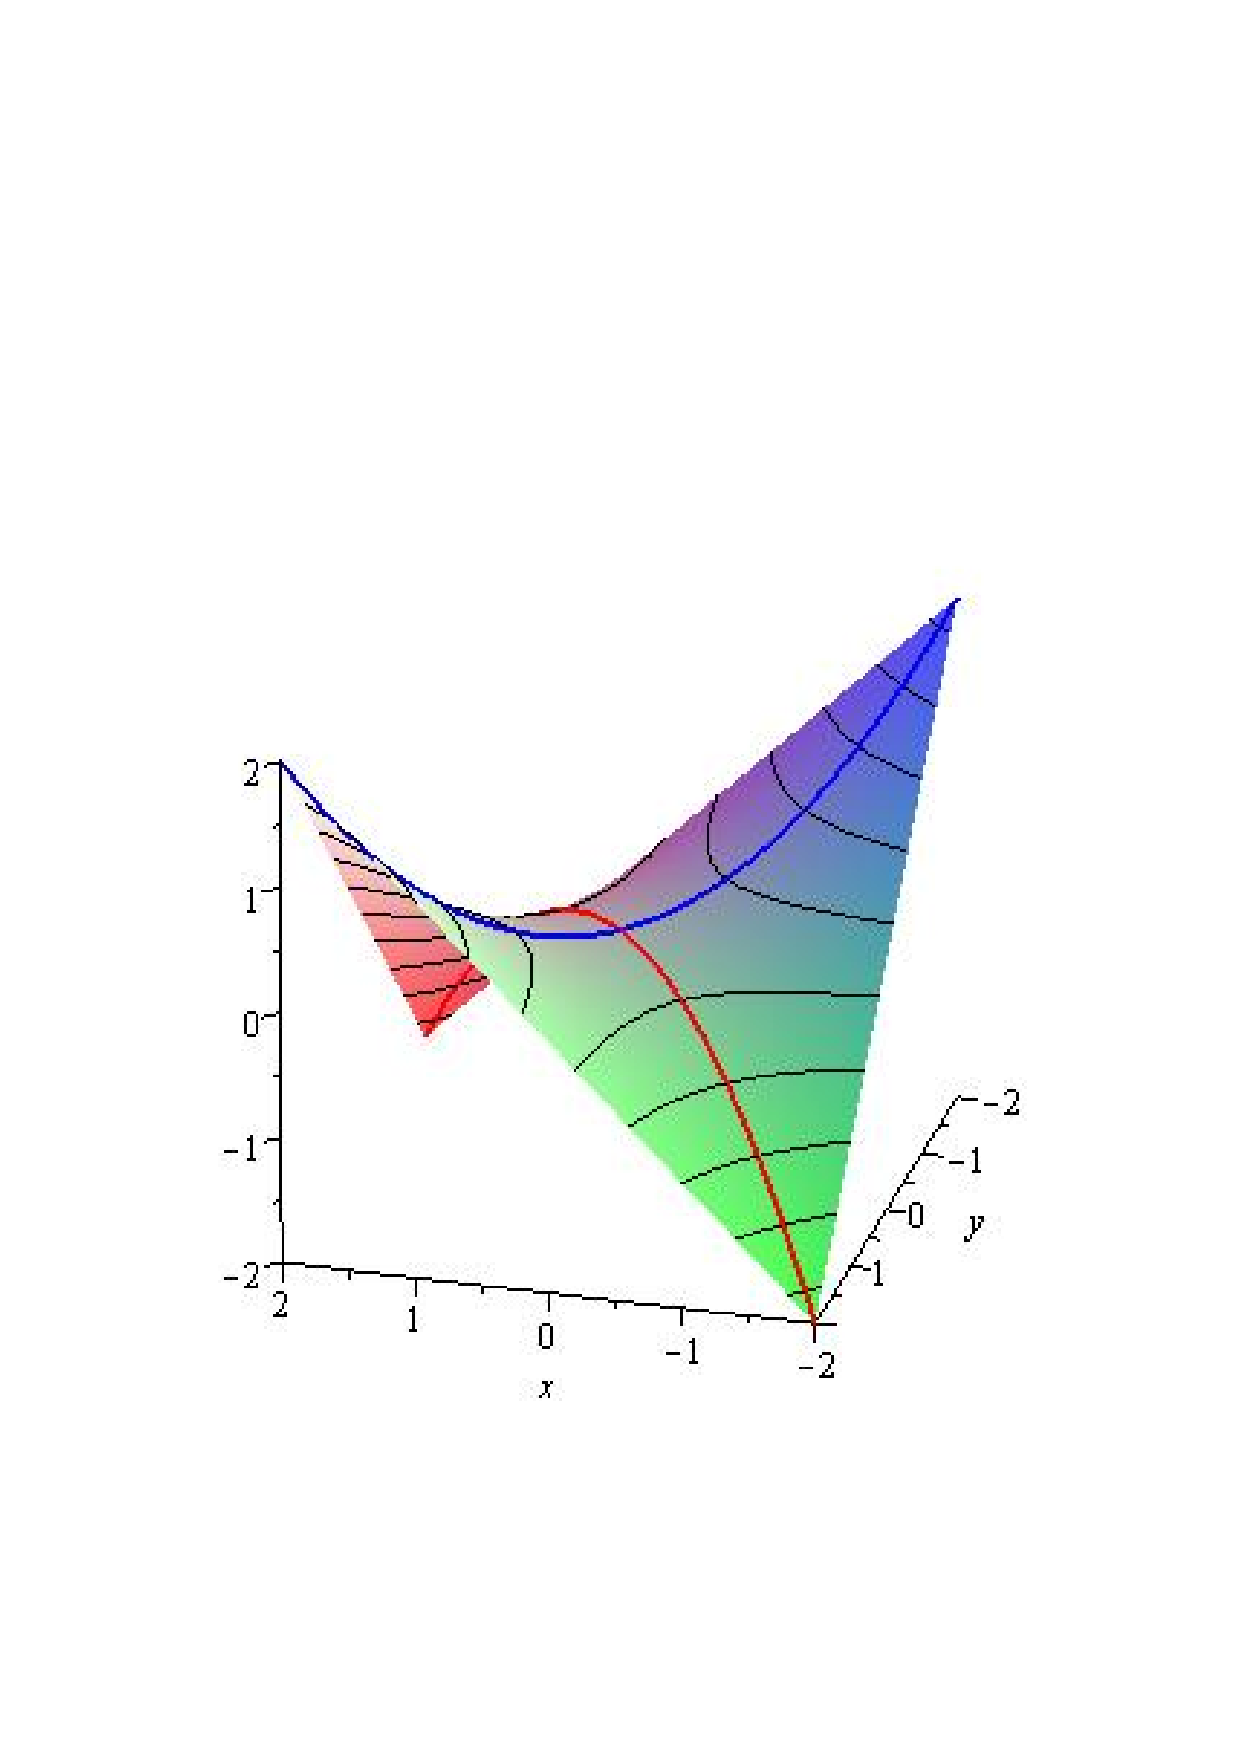
\includegraphics[clip,trim=2cm 2cm 2cm 2cm,scale=0.25]{images/saddle.jpg}
 \end{center}
 \uncover<2->{If we walk along the blue curve, the saddle looks like a
  local minimum.  }\uncover<3->{If we walk along the red curve, it
  looks like a local maximum instead.  }\uncover<4->{Saddle points are 
  common, not like inflection points.  }\uncover<5->{If we have found
  a critical point and we want to know whether it is a local maximum,
  a local minimum or a saddle, we need to look at the Hessian matrix.}
\end{frame}

\begin{frame}[t]
 \frametitle{Classifying critical points}
 \begin{itemize}
  \item<1-> Suppose $f(x,y)$ has a critical point at $(a,b)$ (so
   $f_x(a,b)=f_y(a,b)=0$).  \uncover<2->{Consider the Hessian matrix 
   \[ H = \bbm f_{xx}(a,b) & f_{xy}(a,b) \\
               f_{xy}(a,b) & f_{yy}(a,b) \ebm
        \uncover<3->{= \bbm p & q \\ q & r \ebm \text{ say. }}
   \]}
  \item<4-> The \emph{eigenvalues} of $H$ are the numbers
   \[ e_1 = (p+r-\sqrt{(p-r)^2+4q^2})/2 \hspace{4em}
      e_2 = (p+r+\sqrt{(p-r)^2+4q^2})/2.
   \]
  \item<5-> If $e_1,e_2<0$ then there is a local maximum at $(a,b)$.
  \item<6-> If $e_1<0<e_2$ then there is a saddle point at $(a,b)$.
  \item<7-> If $0<e_1,e_2$ then there is a local minimum at $(a,b)$.
  \item<8-> In the rare case where $e_1=0$ or $e_2=0$, the situation
   is more complicated (as with inflection points).
  \item<9-> Alternatively, put $A_1=f_{xx}(a,b)=p$ and
   $A_2=\det(H)=pr-q^2$.
  \item<10-> If $A_2>0$ and $A_1<0$ there is a local maximum.
  \item<11-> If $A_2>0$ and $A_1>0$ there is a local minimum.
  \item<12-> If $A_2<0$ there is a saddle point.
 \end{itemize}
\end{frame}

\begin{frame}[t]
 \frametitle{The function $f(x,y)=x^3+3xy+y^3$}
 \begin{itemize}
  \item<1-> Take $f(x,y)=x^3+3xy+y^3$.  \uncover<2->{
   The derivatives are 
   \begin{align*}
    \uncover<3->{f_x(x,y)} &\uncover<3->{= 3x^2+3y} & & &
    \uncover<4->{f_y(x,y)} &\uncover<4->{= 3x+3y^2} \\
    \uncover<5->{f_{xx}(x,y)} &\uncover<5->{= 6x} &
    \uncover<6->{f_{xy}(x,y)} &\uncover<6->{= 3} & 
    \uncover<7->{f_{yy}(x,y)} &\uncover<7->{= 6y.} 
   \end{align*}
  }
  \item<8-> At a critical point we must have $3x^2+3y=0$ and
   $3x+3y^2=0$\uncover<9->{, so $y=-x^2$ and $x=-y^2$.}
   \uncover<10->{This gives $x=-y^2=-(-x^2)^2=-x^4$}\uncover<11->{, so 
   $x^4+x=0$}\uncover<12->{, so $x(x^3+1)=0$}\uncover<13->{, so 
   $x=0$ or $x=-1$.}\uncover<14->{ We also have $y=-x^2$, so if $x=0$
   we have $y=0$, and if $x=-1$ we have $y=-1$.}\uncover<15->{ This 
   means that the critical points are $(0,0)$ and $(-1,-1)$.}
  \item<16-> $H=\bbm f_{xx}&f_{xy}\\f_{xy}&f_{yy}\ebm
   \uncover<17->{=\bbm 6x&3\\3&6y\ebm}$\uncover<18->{\\
    $A_1=6x$}\uncover<19->{; $A_2=6x\tm 6y-3\tm 3=9(4xy-1)$}
  \item<20-> At $(0,0)$: $A_2=-9<0$ so we have a saddle point.
  \item<21-> At $(-1,-1)$: $A_2=27>0$, $A_1=-6<0$ so we have a 
   local maximum.
 \end{itemize}
\end{frame}

\begin{frame}[t]
 \frametitle{The function $f(x,y)=x^3+3xy+y^3$}
 $f=x^3+3xy+y^3$; saddle point at $(0,0)$; local maximum at
 $(-1,-1)$. 
 \uncover<2->{
 \[ \includegraphics[scale=0.15]{images/poly_crit_i.jpg} 
     \hspace{3em}
    \includegraphics[scale=0.15]{images/poly_crit_i_contour.jpg} 
 \]}
 \uncover<3->{\vspace{-1ex}\hrule
 \vspace{1ex}
 $H=\bbm f_{xx}&f_{xy}\\f_{xy}&f_{yy} \ebm$}\uncover<4->{; 
 $A_1=f_{xx}$}\uncover<5->{; $A_2=\det(H)=f_{xx}f_{yy}-f_{xy}^2$}\\
 \uncover<6->{$A_2<0$: saddle}\uncover<7->{; $A_1,A_2>0$:
 local minimum}\uncover<8->{; $A_1<0$, $A_2>0$: local maximum.}
 \uncover<9->{\vspace{1ex}
 \hrule
 \vspace{1ex}
 For $f$ as above: $A_1=6x$, $A_2=9(4xy-1)$.\\}
 \uncover<10->{At $(0,0)$: $A_1=0$, $A_2=-9<0$, saddle point.\\}
 \uncover<11->{At $(-1,1)$: $A_1=-6<0$, $A_2=27>0$, local maximum.\\}
\end{frame}

\begin{frame}[t]
 \frametitle{The function $\sin(x)\sin(y)$}
 
 \begin{itemize}
  \item<1-> Put $f(x,y)=\sin(x)\sin(y)$.\uncover<2->{
   The derivatives are
   \begin{align*}
    \uncover<3->{f_x(x,y)} &\uncover<3->{= \cos(x)\sin(y)} & & &
    \uncover<4->{f_y(x,y)} &\uncover<4->{= \sin(x)\cos(y)} \\
    \uncover<5->{f_{xx}(x,y)} &\uncover<5->{= -\sin(x)\sin(y)} & 
    \uncover<6->{f_{xy}(x,y)} &\uncover<6->{= \cos(x)\cos(y)} & 
    \uncover<7->{f_{yy}(x,y)} &\uncover<7->{= -\sin(x)\sin(y).} 
   \end{align*}
  }
  \item<8-> At a critical point, we must have $\cos(x)\sin(y)=0$
   and $\sin(x)\cos(y)=0$.  \only<9>{Thus one of the following holds:
   \[ \begin{array}{lll}
        (p):\qquad \cos(x)=\sin(x)=0 & \hspace{4em} &
        (q):\qquad \cos(x)=\cos(y)=0 \\
        (r):\qquad \sin(y)=\sin(x)=0 & \hspace{4em} &
        (s):\qquad \sin(y)=\cos(y)=0.
      \end{array}
   \]
   \WHITE{but~(p) and~(s) cannot happen, because $\sin^2+\cos^2=1$.}
   }\only<10->{Thus one of the following holds:
   \[ \begin{array}{lll}
        \GRAY{(p):\qquad \cos(x)=\sin(x)=0} & \hspace{4em} &
        (q):\qquad \cos(x)=\cos(y)=0 \\
        (r):\qquad \sin(y)=\sin(x)=0 & \hspace{4em} &
        \GRAY{(s):\qquad \sin(y)=\cos(y)=0.}
      \end{array}
   \]
   but~(p) and~(s) cannot happen, because $\sin^2+\cos^2=1$.
   }
  \item<11-> 
   $\sin(t)=0$ for $t=n\pi$; $\cos(t)=0$ for $t=(n+\half)\pi$.
   \begin{center}
    \begin{tikzpicture}
     \draw[->] (-3,0) -- (3.2,0);
     \draw[->] (0,-1.1) -- (0,1.1);
     \draw[red,domain=-3:3,samples=300,smooth,variable=\x]
        plot({\x},{sin(180*\x)});
     \draw[blue,domain=-3:3,samples=300,smooth,variable=\x]
        plot({\x},{cos(180*\x)});
     \foreach \x in {-3,-2,-1,0,1,2,3} {
      \draw (\x,0) -- (\x,-0.1);
     }
     \draw(-3,-0.18) node{$\ss -3\pi$};
     \draw(-2,-0.18) node{$\ss -2\pi$};
     \draw(-1,-0.18) node{$\ss -\pi$};
     \draw( 0,-0.18) node{$\ss 0$};
     \draw( 1,-0.18) node{$\ss \pi$};
     \draw( 2,-0.18) node{$\ss 2\pi$};
     \draw( 3,-0.18) node{$\ss 3\pi$};
     \draw[blue] (3.05,-0.9) node[anchor=west]{$\ss y=\cos(x)$};
     \draw[red]  (3.05, 0.9) node[anchor=west]{$\ss y=\sin(x)$};
    \end{tikzpicture}
   \end{center}
 \end{itemize}
\end{frame}

\begin{frame}[t]
 \frametitle{The function $\sin(x)\sin(y)$}
 $f(x,y)=\sin(x)\sin(y)$;
 $f_x(x,y)=\cos(x)\sin(y)$;
 $f_y(x,y)=\sin(x)\cos(y)$. \\
 At critical point, either (r): $\sin(x)=\sin(y)=0$ or 
 (q): $\cos(x)=\cos(y)=0$. \\
 $\sin(t)=0$ for $t=n\pi$; $\cos(t)=0$ for $t=(n+\half)\pi$. \\[1ex]
 \hrule
 \vspace{1ex}
 \begin{itemize}
  \item<2-> In case (r): $x=n\pi$ and $y=m\pi$ for some integers $n,m$. 
  \item<3-> In case (q): $x=(n+\half)\pi$ and $y=(m+\half)\pi$ for
   some integers $n,m$.
  \item<4-> $H=\bbm -\sin(x)\sin(y)&\cos(x)\cos(y) \\
                    \cos(x)\cos(y)&-\sin(x)\sin(y) \ebm
            $
  \item<5->{$A_1=-\sin(x)\sin(y)$}\uncover<6->{; 
    $A_2=\sin(x)^2\sin(y)^2-\cos(x)^2\cos(y)^2$.
   }
  \item<7-> At $(n\pi,m\pi)$: $A_2=-1<0$, so we have a saddle point.
  \item<8-> Note that $\cos((k+\half)\pi)=0$, $\sin((k+\half)\pi)=(-1)^k$.
  \item<9-> At $((n+\half)\pi,(m+\half)\pi)$: $A_1=(-1)^{n+m+1}$, 
   $A_2=1>0$.
  \item<10-> If $n+m$ is even: $A_1=-1<0$ and $A_2=1>0$ so we have a local maximum.
  \item<11-> If $n+m$ is odd: $A_1=1>0$ and $A_2=1>0$ so we have a local minimum.
 \end{itemize}
\end{frame}


\begin{frame}[t]
 \frametitle{The function $\sin(x)\sin(y)$}
 \only<1>{
 \[ \includegraphics[clip,trim=1cm 7cm 1cm 9cm,scale=0.3]{images/sinsin_crit.jpg} \]
 }
 \only<2>{
 \[ \includegraphics[clip,trim=1cm 7cm 1cm 9cm,scale=0.3]{images/sinsin_saddle.jpg} \]
 }
 \only<3>{
 \[ \includegraphics[clip,trim=1cm 7cm 1cm 9cm,scale=0.3]{images/sinsin_max.jpg} \]
 }
 \only<4>{
 \[ \includegraphics[clip,trim=1cm 7cm 1cm 9cm,scale=0.3]{images/sinsin_min.jpg} \]
 }
 \begin{itemize}
  \item<2-> There are saddle points at $(n\pi,m\pi)$ for all integers $n$ and $m$.
  \item<3-> There is a local maximum at $((n+\half)\pi,(m+\half)\pi)$ whenever $n+m$ is even.
  \item<4-> There is a local minimum at $((n+\half)\pi,(m+\half)\pi)$ whenever $n+m$ is odd.
 \end{itemize}
\end{frame}

\begin{frame}[t]
 \frametitle{The function $e^{-x^2-y^2-2y}$}
 
 \begin{itemize}
  \item<1-> Take $f(x,y)=e^{-x^2-y^2-2y}$.
  \item<2-> $f_x=-2xe^{-x^2-y^2-2y}\uncover<3->{=-2xf}$
  \item<4-> $f_y=(-2y-2)e^{-x^2-y^2-2y}\uncover<5->{=(-2y-2)f}$
  \item<6-> For a critical point, we must have $-2xf=0$ and $(-2y-2)f=0$.
   \uncover<7->{Here $f$ is never zero, so $-2x=-2y-2=0$ so $(x,y)=(0,-1)$.}
  \item<8-> $f_{xx}=(-2xf)_x\uncover<9->{=-2f-2xf_x}\uncover<10->{=-2f+4x^2f}\uncover<11->{=(4x^2-2)f}$
  \item<12-> $f_{xy}=(-2xf)_y\uncover<13->{=-2xf_y}\uncover<14->{=-2x(-2y-2)f}\uncover<15->{=(4xy+4x)f}$
  \item<16-> $f_{yy}=((-2y-2)f)_y\uncover<17->{=-2f+(-2y-2)f_y}\uncover<18->{=-2f+(2y+2)^2f}\uncover<19->{=(4y^2+8y+2)f}$
  \item<20-> At the critical point $(x,y)=(0,-1)$ we have
    $f=e^{-0-1+2}=e$ \uncover<21->{so 
   \[ H = \bbm f_{xx} & f_{xy} \\ f_{xy} & f_{yy} \ebm 
         \uncover<22->{= \bbm 4x^2-2 & 4xy+4x \\ 4xy+4x & 4y^2+8y+2 \ebm f }
         \uncover<23->{= \bbm -2e & 0 \\ 0 & -2e \ebm }
   \]}
  \item<24-> Now $A_1=-2e<0$ and $A_2=(-2e)^2-0^2=4e^2>0$ so we have
   a local maximum at $(0,-1)$.
 \end{itemize}
\end{frame}

\begin{frame}[t]
 \frametitle{The function $e^{-x^2-y^2-2y}$}
 \[ 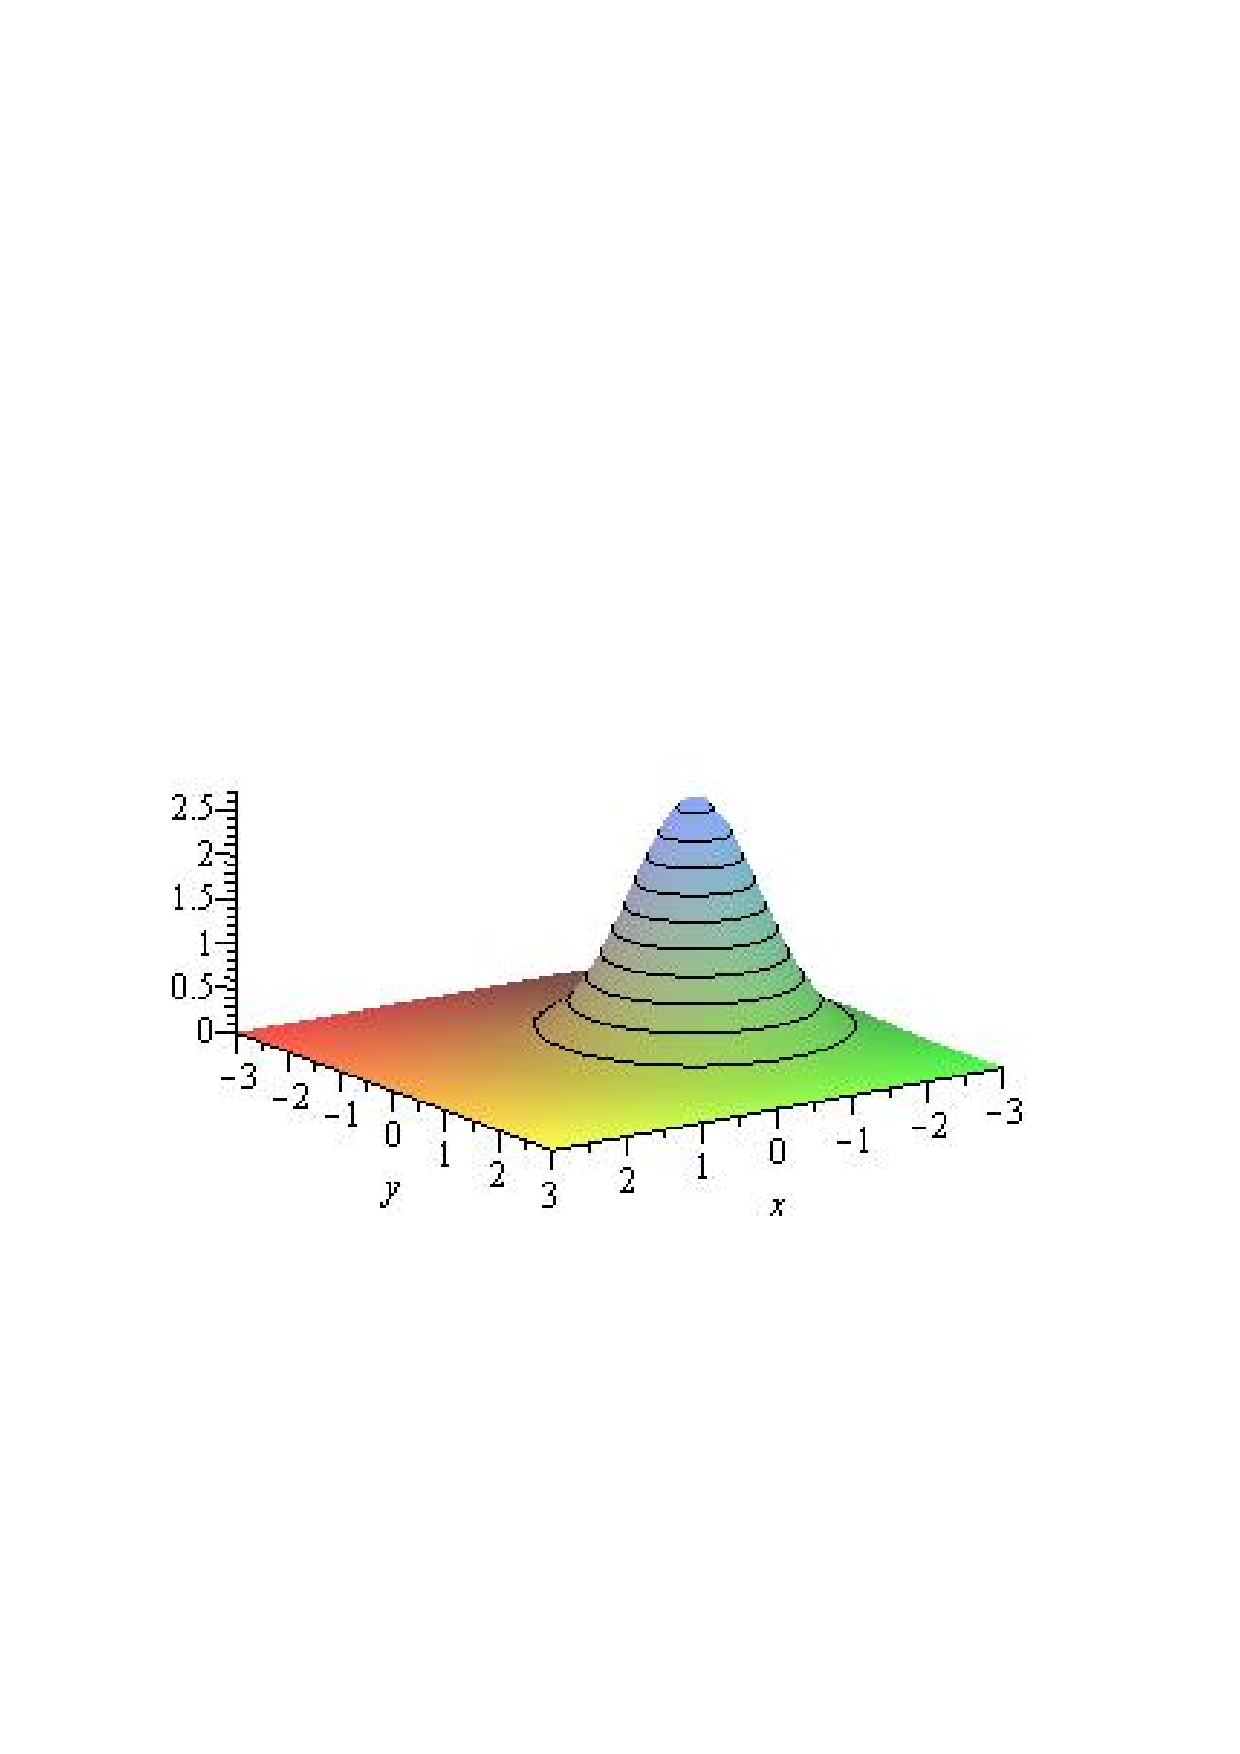
\includegraphics[clip,trim=1cm 4cm 1cm 4cm,scale=0.5]{images/gauss_crit.jpg} \]
 There is a local maximum at $(0,-1)$ and no other critical points.
\end{frame}

\begin{frame}[t]
 \frametitle{Complications}
 
 \begin{itemize}
  \item<1-> As in the one-variable case, there are complications in
   the relationship between critical points and maxima/minima.
  \item<2-> The function may not have a maximum or minimum.
  \item<3-> It may have a maximum or minimum that is approached
   arbitrarily closely, but never actually reached.
  \item<4-> A function defined on a restricted region may have a
   maximum or minimum on the boundary of that region, and this may
   not be a critical point.
  \item<5-> Differential methods may not work well for functions that
   are not sufficiently smooth.
  \item<6-> These phenomena can be important, but we will not discuss
   them further here.
 \end{itemize}
\end{frame}


\begin{frame}[t]
 \frametitle{More variables}
 \begin{itemize}
  \item<1-> Not very much changes if there are more than two variables.
  \item<2-> Critical points are points where all partial derivatives vanish.
  \item<3-> Local maxima and minima are always critical points.
  \item<4-> There may be other critical points, which are saddles of
   various kinds.
  \item<5-> If there are $n$ variables, then the Hessian is an $n\tm n$
   symmetric matrix.
  \item<6-> If all the eigenvalues are positive, we have a local minimum.
   \uncover<7->{If all are negative, we have a local maximum.}
   \uncover<8->{If some are negative and some are positive, we have a saddle.}
  \item<9-> Let $A_k$ be the determinant of the top left $k\tm k$
   block in the Hessian.  \uncover<10->{If the variables are $w,x,y,z$ we have 
    {\tiny \[ A_1 = f_{ww} \hspace{1em}
       A_2 = \det\bbm f_{ww} & f_{wx} \\ f_{xw} & f_{xx}\ebm \hspace{1em} 
       A_3 = \det\bbm f_{ww} & f_{wx} & f_{wy} \\
                      f_{xw} & f_{xx} & f_{xy} \\
                      f_{yw} & f_{yx} & f_{yy} \ebm \hspace{1em} 
       A_4 = \det\bbm f_{ww} & f_{wx} & f_{wy} & f_{wz} \\
                      f_{xw} & f_{xx} & f_{xy} & f_{xz} \\
                      f_{yw} & f_{yx} & f_{yy} & f_{yz} \\
                      f_{zw} & f_{zx} & f_{zy} & f_{zz} \ebm
    \]}
   }
  \item<11-> If all $A_k$ are positive we have a local minimum.  
   \uncover<12->{If $A_1<0$, $A_2>0$, $A_3<0$, $A_4>0$ etc then we
    have a local maximum. }\uncover<13->{Otherwise, provided that the last
    $A$ is nonzero, we have a saddle.} 
 \end{itemize}
\end{frame}


\begin{frame}
 \frametitle{An example with three variables}
 
 \begin{itemize}
  \item<1-> Take $f(x,y,z)=8(x^2+y^2+z^2)-(z+1)^3$
  \item<2-> We have $f_x=16x$\uncover<3->{ and $f_y=16y$}\uncover<4->{ and 
   \[ f_z = 16z - 3(z+1)^2
       \uncover<5->{ = 16z - 3z^2 - 6z - 3}
       \uncover<6->{ = -3+10z-3z^2}
       \uncover<7->{ = (z-3)(1-3z).}
   \]}
  \item<8-> We have critical points where $x=y=0$ and
   $(z-3)(1-3z)=0$ \uncover<9->{ so $z=3$ or $z=1/3$.}
  \item<10-> The Hessian matrix is 
   \[ H = \bbm f_{xx} & f_{xy} & f_{xz} \\
               f_{yx} & f_{yy} & f_{yz} \\
               f_{zx} & f_{zy} & f_{zz} \ebm 
      \uncover<11->{=
          \bbm 16 & 0  & 0 \\
               0  & 16 & 0 \\
               0  & 0  & 10-6z \ebm}
   \]
  \item<12-> $A_1=16$ \uncover<13->{ and $A_2=256$} \uncover<14->{ and $A_3=256(10-6z)$.}
  \item<15-> At $(0,0,1/3)$ we get $A_3=2048$ so $A_1$, $A_2$ and
   $A_3$ are all positive, so we have a local minimum.
  \item<16-> At $(0,0,3)$ we have $A_3=-2048\neq 0$ and the signs
   do not alternate so we have some kind of saddle.
 \end{itemize}
\end{frame}

\begin{frame}[t]
 \frametitle{Constrained optimisation}
 \begin{itemize}
  \item<1-> So far we have tried to find the maximum value of a
   function $f(x,y)$, where both $x$ and $y$ can vary freely.
  \item<2-> This is like looking for the highest point in a certain
   area of land.
  \item<3-> What if we want to find the highest point on the road
   instead?
  \item<4-> The road will be given by some equation which we can put
   in the form $g(x,y)=0$.  For example, $g(x,y)=x^2+y^2-4$
   corresponds to a circular road, and $g(x,y)=x+y-6$ corresponds to
   an infinite straight road.
  \item<5-> We want to maximise $f(x,y)$ subject to the constraint
   $g(x,y)=0$.
  \item<6-> The maximum and minimum occur at points where the road
   is tangent to the contours.
   \[ \includegraphics[clip,trim=4cm 0cm 0cm 8cm,scale=0.18]{images/lg_skirt.jpg}
      \hspace{4em}
      \includegraphics[scale=0.12]{images/lg_contour.jpg}
   \]
 \end{itemize}
\end{frame}

\begin{frame}[t]
 \frametitle{Constrained optimisation - applications}

 \begin{itemize}
  \item<1-> Suppose we want to build a 5kW motor that
   is as light as possible.  We have come up with a design with
   parameters $a$, $b$ and $c$ that we can adjust.  The weight is
   $W(a,b,c)$ and the power (in kW) is $P(a,b,c)$.  We want to
   minimise $W(a,b,c)$ subject to the constraint $P(a,b,c)-5=0$.
  \item<2-> More generally, whenever we design a device, there will be
   some requirements that are not negotiable; these will be expressed
   by constraint equations.  There will be other functions that
   measure the effectiveness of the device.  We want to maximise
   these, but we have to do so subject to the constraints.
 \end{itemize}
\end{frame}


\begin{frame}[t]
 \frametitle{The Lagrange multiplier method}
 \begin{itemize}
  \item<1-> To maximise or minimise $f(x,y)$ subject to $g(x,y)=0$, we
   find the (unconstrained) critical points of the function
   $L(\lm,x,y)=f(x,y)-\lm g(x,y)$.
  \item<2-> For example, suppose we want to minimise $f(x,y)=x^2+y^2$
   subject to $3x+4y=5$.  \uncover<3->{Then $g(x,y)=3x+4y-5$ so 
   \[ L(\lm,x,y) = x^2+y^2-\lm(3x+4y-5). \]}
  \item<4-> For a critical point, the derivatives must vanish:
   \begin{align*}
    L_\lm &= -3x-4y+ 5 = 0 \tag{A} \\
    L_x   &= 2x-3\lm = 0 \tag{B} \\
    L_y   &= 2y-4\lm = 0. \tag{C}
   \end{align*}
  \item<5-> Here~(B) and~(C) give $x=3\lm/2$ and $y=2\lm$.
   \uncover<6->{Substituting these values in~(A) gives
    $-9\lm/2-8\lm+5=0$}\uncover<7->{, which simplifies to
    $\lm=2/5$.}\uncover<8->{  This in turn gives $x=3\lm/2=3/5$ and
    $y=2\lm=4/5$.}\uncover<9->{  Thus, the only critical point is
    $(x,y)=(3/5,4/5)$.}\uncover<10->{  The value of $f$ here is
    $(3/5)^2+(4/5)^2=1$. } 
 \end{itemize}
\end{frame}

\begin{frame}[t]
 \frametitle{Geometric interpretation}
  $f(x,y)=x^2+y^2=\text{ squared distance from $(x,y)$ to $(0,0)$}$\\
  $g(x,y)=3x+4y-5=0$; minimum value of $f$ is $1$ at $(3/5,4/5)$.
  \par\medskip\hrule\medskip\par
  \uncover<2->{
   Geometrically, we have found the closest point to the origin on the
   line $3x+4y=5$.
   \begin{center}
    \begin{tikzpicture}[scale=1.3]
     \draw[->] (-2,0) -- (2,0);
     \draw[->] (0,-2) -- (0,2);
     \draw[dotted,blue] (0,0) circle(0.2);
     \draw[dotted,blue] (0,0) circle(0.4);
     \draw[dotted,blue] (0,0) circle(0.6);
     \draw[dotted,blue] (0,0) circle(0.8);
     \draw[dotted,blue] (0,0) circle(1.2);
     \draw[dotted,blue] (0,0) circle(1.4);
     \draw[dotted,blue] (0,0) circle(1.6);
     \fill[white] (0.5,0.7) rectangle (2,0.9); 
     \draw[red] (-1,2) -- (2,-0.25);
     \draw[       blue] (0,0) circle(1.0);
     \fill (0.6,0.8) circle(0.03);
     \draw(0.7,0.8) node[anchor=west] {$(3/5,4/5)$};
     \draw(2,-0.25) node[anchor=north west] {$3x+4y-5=0$};
    \end{tikzpicture}
   \end{center}
  }
\end{frame}

\begin{frame}[t]
 \frametitle{Why does the method (usually) work?}
 \begin{itemize}
  \item<1-> Suppose that $(\lm,x,y)$ is a critical point for
   $L(\lm,x,y)=f(x,y)-\lm g(x,y)$.
  \item<2-> We have $L_\lm(\lm,x,y)=-g(x,y)$, and this must be zero as
   we are at a critical point of $L$.  This means that we are on the
   constraint curve.
  \item<3-> We also have $L_x=L_y=0$, which means that $f_x=\lm g_x$
   and $f_y=\lm g_y$ (at this point).
  \item<4-> Now suppose we move a little way along the constraint
   curve, by $(\dl x,\dl y)$ say.
  \item<5-> The change in $g$ is $\dl x.g_x+\dl y.g_y$.
  \item<6-> As we are staying on the constraint curve, $g$ is still
   zero, so we must have $\dl x.g_x+\dl y.g_y=0$.  
  \item<7-> This means that
   $\dl x.\lm g_x+\dl y.\lm g_y=0$\uncover<8->{, so 
   $\dl x.f_x+\dl y.f_y=0$}\uncover<9->{, so $\dl f=0$.}
  \item<8-> We see from this that $(x,y)$ is a critical point for the
   constrained problem.
  \item<9-> Geometrically, the vector $\vu=\bbm g_x\\ g_y\ebm$ is normal
   to the constraint curve, and $\vv=\bbm f_x\\ f_y\ebm$ is normal to
   the contour of $f$.  The equations $f_x=\lm g_x$ and $f_y=\lm g_y$
   say that $\vv$ is a multiple of $\vu$, so the constraint curve is
   running parallel to the contour.
 \end{itemize}
\end{frame}

\begin{frame}[t]
 \frametitle{A constrained optimization example}
 \begin{tabular}{ll}
  \parbox[t]{7cm}{
   Consider a metal tank, open at the top.
   The volume is $V=xyz$, and the area is $S=xy+2xz+2yz$.
   We want the volume to be $4m^3$, and we want to minimise $S$, to use
   as little metal as possible.
  } & \parbox[t]{4cm}{
  \begin{center}
   \begin{tikzpicture}
    \draw (0,0) -- (2,0) -- (2,1) -- (0,1) -- (0,0);
    \draw (0,0) -- (0,1) -- (-0.8,1.6) -- (-0.8,0.6) -- (0,0);
    \draw (0,1) -- (-0.8,1.6) -- (1.2,1.6) -- (1.2,1) -- (0,1);
    \draw (1.2,1.6) -- (2,1) -- (1.2,1) -- (1.2,1.6);  
    \draw (-0.45, 0.2) node{$\ss x$}; 
    \draw ( 1.0,-0.2) node{$\ss y$}; 
    \draw ( 2.1, 0.5) node{$\ss z$}; 
   \end{tikzpicture}
  \end{center}}
 \end{tabular}
 \vspace{-5ex}
 \begin{itemize}
  \item<2-> We are minimising $S$ subject to $V-4=0$, so
   $L=xy+2xz+2yz-\lm(xyz-4)$.
  \item<3-> Equations are
   \begin{align*}
    L_\lm &= 4-xyz = 0 & \uncover<4->{xyz} & \uncover<4->{=4} \tag{A} \\
    L_x   &= y+2z-\lm yz=0  &
      \uncover<5->{z^{-1}+2y^{-1}} & \uncover<5->{=\lm} \tag{B} \\
    L_y   &= x+2z-\lm xz=0  &
      \uncover<6->{z^{-1}+2x^{-1}} & \uncover<6->{=\lm} \tag{C} \\
    L_z   &= 2x+2y-\lm xy=0  &
      \uncover<7->{2y^{-1}+2x^{-1}} & \uncover<7->{=\lm.} \tag{D}
   \end{align*}
  \item<8-> Subtract~(B) and~(C) to get $x^{-1}=y^{-1}$ so $x=y$.
   \uncover<9->{Substitute in~(D) to get $4x^{-1}=4y^{-1}=\lm$, so $x=y=4/\lm$.}
   \uncover<10->{Substitute in~(C) to get $z^{-1}+\lm/2=\lm$, so $z=2/\lm$.}
   \uncover<11->{Substitute in~(A) to get $32=4\lm^3$, so $\lm=2$\uncover<12->{,
    so $(x,y,z)=(2,2,1)$.}}
  \item<13-> For these values, we have $S=12$.  Thus, the minimum
   possible area of metal sheet that we need is $12m^2$.
 \end{itemize}
\end{frame}

\begin{frame}[t]
 \frametitle{A constrained optimisation example}
 \begin{itemize}
  \item<1-> Problem: maximise $f(x,y)=x+y$ subject to $x^2/a+y^2/b=1$\\
   (for some constants $a,b>0$).
  \item<2-> Take $L=x+y-\lm(x^2/a+y^2/b-1)$.  For a critical point:
   \begin{align*}
    L_\lm &= 1-x^2/a-y^2/b = 0 & x^2/a+y^2/b &= 1 \tag{A} \\
    L_x &= 1-2x\lm/a = 0 & x &= a/(2\lm) \tag{B} \\
    L_y &= 1-2y\lm/b = 0 & y &= b/(2\lm) \tag{C}.
   \end{align*}
  \item<3-> Substitute~(B) and~(C) in~(A) to get $(a+b)/(4\lm^2)=1$,
   so $\lm=\pm\sqrt{a+b}/2$.  \uncover<4->{As $x=a/(2\lm)$ and
   $y=b/(2\lm)$ this gives 
   \[ (x,y) = \pm \left(\frac{a}{\sqrt{a+b}},\frac{b}{\sqrt{a+b}}\right).
   \]}
  \item<5->  For these points we have 
   \[ f(x,y)=x+y=\pm(a+b)/\sqrt{a+b} = \pm\sqrt{a+b}. \]
   \uncover<6->{
   This means that the maximum possible value of $f$ (subject to the
   constraint) is $\sqrt{a+b}$, and the minimum is $-\sqrt{a+b}$.}
 \end{itemize}
\end{frame}

\begin{frame}[t]
 \frametitle{A constrained optimisation example}
 Problem: maximise $f(x,y)=x+y$ subject to $x^2/a+y^2/b=1$\\
 Maximum and minimum values are $\pm\sqrt{a+b}$, at the
 points $\pm(a,b)/\sqrt{a+b}$. 
 \begin{center}
  \begin{tikzpicture}[scale=1.6]
   \draw[->] (-1.5,0) -- (1.5,0);
   \draw[->] (0,-1.5) -- (0,1.6);
   \foreach \t in {0,0.2,...,3} {
    \draw[blue,dotted] ({\t-1.5},1.5) -- (1.5,{\t-1.5});
    \draw[blue,dotted] ({1.5-\t},-1.5) -- (-1.5,{1.5-\t});
   }
   \fill[white] (0.8,-0.6) rectangle (1.5,-0.9);
   \fill[white] (0.5,1) rectangle (1.5,1.3);
   \draw[blue] ( 0.1, 1.5) -- ( 1.7,-0.1);
   \draw[blue] (-0.1,-1.5) -- (-1.7, 0.1);
   \draw[red,domain=0:360,samples=300,smooth,variable=\t]
    plot({0.96*cos(\t)},{1.28*sin(\t)});
   \fill ( 0.576, 1.024) circle(0.03);
   \fill (-0.576,-1.024) circle(0.03);
   \draw (0.9,-0.75) node[anchor=west]{$g(x,y)=0$};
   \draw ( 1.7,-0.1) node[anchor=west]{$f(x,y)=\sqrt{a+b}$};
   \draw (-1.7, 0.1) node[anchor=east]{$f(x,y)=-\sqrt{a+b}$};
   \draw ( 0.6,1.15) node[anchor=west]{$(a/\sqrt{a+b},b/\sqrt{a+b})$};
  \end{tikzpicture}
 \end{center}
\end{frame}

\begin{frame}[t]
 \frametitle{Several constraints}
 
 \begin{itemize}
  \item<1-> There is a similar method for problems with several
   constraints.
  \item<2-> For example: maximise $z$ subject to $x^2+y^2+z^2=9$ and
   $x+2y+4z=3$.
  \item<3-> Method: find unconstrained critical points of 
   \[ L=z-\lm(x^2+y^2+z^2-9)-\mu(x+2y+4z-3) \]
  \item<4-> Equations: \vspace{-4.5ex}
   \begin{align*}
    L_\lm &= 9-x^2-y^2-z^2=0 \tag{A} \\
    L_\mu &= 3-x-2y-4z=0 \tag{B} \\
    L_x &= -2x\lm- \mu =0 \tag{C} \\
    L_y &= -2y\lm-2\mu =0 \tag{D} \\
    L_z &= -2z\lm-4\mu =0 \tag{E}
   \end{align*}
  \item<5-> These can be solved: use~(B) to eliminate $x$\uncover<6->{
   and~(C) to eliminate $\mu$}\uncover<7->{, then it works out
   that~(D) rearranges to give $y=(6-8z)/5$.}\uncover<8->{
   Substituting these into~(A) gives
   $-21z^2/5+24z/5+36/5=0$}\uncover<9->{, which gives $z=2$ or
   $z=-6/7$.}\uncover<10->{  After a few more steps, we see that the
   solutions are  
   \begin{align*}
    (\lm,\mu,x,y,z) &= (1/12, 1/6, -1, -2, 2) \\
    (\lm,\mu,x,y,z) &= (-1/12, 3/14, 9/7, 18/7, -6/7).
   \end{align*}\vspace{-1ex}}
  \item<11-> Thus, the minimum value of $z$ is $-6/7$ at
   $(9/7,18/7,-6/7)$, and the maximum is $2$ at $(-1,2,2)$.
 \end{itemize}
\end{frame}

\begin{frame}[t]
 \frametitle{Several constraints}

 We wanted to maximise $z$ subject to $x^2+y^2+z^2=9$ and $x+2y+4z=3$.
 \uncover<2->{
 \[
  \includegraphics[clip=true,trim=4cm 4cm 4cm 4cm,scale=0.2]{images/cut_sphere.jpg}
  \includegraphics[clip=true,trim=4cm 4cm 4cm 4cm,scale=0.2]{images/cut_sphere_levels.jpg}
 \]
 The equation $x^2+y^2+z^2=9$ defines a sphere (shown in colour) and 
 $x+2y+4z=3$ defines a plane (shown in grey).  \uncover<3->{The two
  constraints together give the intersection of the sphere and the 
  plane, which is the red curve.} \uncover<4->{The optimisation
  problem is to find the highest and lowest points on that curve.}
  \uncover<5->{The right-hand picture shows the planes $z=-6/7$ 
  and $z=2$, which we saw were the minimum and maximum values.}  
 }
\end{frame}

% \begin{frame}[t]
% \frametitle{}
%  {\Huge
%   \vspace{6ex}
%   \begin{center}
%    Integrals over plane regions
%   \end{center}
%  }
% \end{frame}

\begin{frame}[t]
 \frametitle{Integrals over plane regions}

 Let $D$ be a region in the plane, and let $f(x,y)$ be a function
 defined for points $(x,y)$ in $D$.  \uncover<2->{We define the
  integral $\iint_D f(x,y)dA$ as follows.}\uncover<3->{ First, we
  divide the region $D$ into a large number of small regions
  $D_1,\dotsc,D_N$.}\uncover<4->{ As each region $D_i$ is small, the
  value of $f$ will not change much as we move around
  $D_i$}\uncover<5->{, so it makes approximate sense to talk about the
  value of $f$ on $D_i$ as a single number.}\uncover<6->{  The integral is
  approximately defined by
 \[ \iint_D f(x,y)\,dA = \sum_{i=1}^N 
     (\text{ value of $f$ on $D_i$ }) \times (\text{ area of } D_i).
 \]}\uncover<7->{
 To get the exact value, we divide $D$ into a larger and larger number
 of smaller and smaller pieces, and then pass to the limit. }
\end{frame}


\begin{frame}[t]
 \frametitle{Applications}

 Some applications of this kind of integration are as follows.
 \begin{itemize}
  \item<2->[(a)] Suppose that the region $D$ is a charged plate, and that
   the charge density at a point $(x,y)$ is $q(x,y)$; then the total
   charge is $Q=\iint_Dq(x,y)\,dA$.
  \item<3->[(b)] Suppose that the region $D$ represents a structure of
   constant density $\rho$ and vertical thickness $f(x,y)$ attached to
   an axle passing vertically through the origin.  \uncover<4->{Then
   the mass of the structure is $\iint_D\rho
   f(x,y)\,dA$}\uncover<5->{, whereas the moment of 
   inertia (which measures the difficulty of turning the axle) is
   $\iint_D\rho f(x,y)(x^2+y^2)dA$.}
  \item<6->[(c)] Suppose that the region $D$ represents a large solar cell,
   with the brightness of light arriving at $(x,y)$ being given by the
   function $f(x,y)$.  Then the total incident power on the cell will
   be (a constant times) $\iint_Df(x,y)\,dA$.  
  \item<7->[(d)] The total area of a region $D$ is just $\iint_D 1\,dA$.
 \end{itemize}

\end{frame}

\begin{frame}[t]
 \frametitle{Rectangular regions}

 In the simplest case, the region $D$ is a rectangle aligned with the
 axes, given by $a\leq x\leq b$ and $c\leq y\leq d$ say.\uncover<2->{ In this case
 we can just divide the horizontal interval $[a,b]$ into small
 intervals of length $\dl x$}\uncover<3->{, and divide the vertical interval $[c,d]$
 into small intervals of length $\dl y$.}\uncover<4->{ This divides $D$ into small
 rectangles of area $\dl A=\dl x.\dl y$.}
 \only<1>{\begin{center}
  \begin{tikzpicture}[scale=1.5]
   \draw[->] (-0.1,0) -- (3.1,0);
   \draw[->] (0,-0.1) -- (0,2.1);
   \fill[green!20] (0.7,0.4) rectangle(2.8,1.6);
   \draw[gray] (0.7,0) -- (0.7,1.6);
   \draw[gray] (2.8,0) -- (2.8,1.6);
   \draw[gray] (0,0.4) -- (2.8,0.4);
   \draw[gray] (0,1.6) -- (2.8,1.6);
   \fill[black] (0.7,0) circle(0.02);
   \fill[black] (2.8,0) circle(0.02);
   \fill[black] (0,0.4) circle(0.02);
   \fill[black] (0,1.6) circle(0.02);
   \draw (0.7,-0.15) node{$a$};
   \draw (2.8,-0.15) node{$b$};
   \draw (-0.15,0.4) node{$c$};
   \draw (-0.15,1.6) node{$d$};
  \end{tikzpicture}
 \end{center}}\only<2>{\begin{center}
  \begin{tikzpicture}[scale=1.5]
   \draw[->] (-0.1,0) -- (3.1,0);
   \draw[->] (0,-0.1) -- (0,2.1);
   \fill[green!20] (0.7,0.4) rectangle(2.8,1.6);
   \draw[gray] (0.7,0) -- (0.7,1.6);
   \draw[gray] (2.8,0) -- (2.8,1.6);
   \draw[gray] (0,0.4) -- (2.8,0.4);
   \draw[gray] (0,1.6) -- (2.8,1.6);
   \fill[black] (0.7,0) circle(0.02);
   \fill[black] (2.8,0) circle(0.02);
   \fill[black] (0,0.4) circle(0.02);
   \fill[black] (0,1.6) circle(0.02);
   \draw (0.7,-0.15) node{$a$};
   \draw (2.8,-0.15) node{$b$};
   \draw (-0.15,0.4) node{$c$};
   \draw (-0.15,1.6) node{$d$};
   \foreach \x in {1.0,1.3,1.6,1.9,2.2,2.5} {
    \draw[dotted] (\x,0) -- (\x,1.6);
   }
  \end{tikzpicture}
 \end{center}}\only<3>{\begin{center}
  \begin{tikzpicture}[scale=1.5]
   \draw[->] (-0.1,0) -- (3.1,0);
   \draw[->] (0,-0.1) -- (0,2.1);
   \fill[green!20] (0.7,0.4) rectangle(2.8,1.6);
   \draw[gray] (0.7,0) -- (0.7,1.6);
   \draw[gray] (2.8,0) -- (2.8,1.6);
   \draw[gray] (0,0.4) -- (2.8,0.4);
   \draw[gray] (0,1.6) -- (2.8,1.6);
   \fill[black] (0.7,0) circle(0.02);
   \fill[black] (2.8,0) circle(0.02);
   \fill[black] (0,0.4) circle(0.02);
   \fill[black] (0,1.6) circle(0.02);
   \draw (0.7,-0.15) node{$a$};
   \draw (2.8,-0.15) node{$b$};
   \draw (-0.15,0.4) node{$c$};
   \draw (-0.15,1.6) node{$d$};
   \foreach \x in {1.0,1.3,1.6,1.9,2.2,2.5} {
    \draw[dotted] (\x,0) -- (\x,1.6);
   }
   \foreach \y in {0.6,0.8,1.0,1.2,1.4} {
    \draw[dotted] (0,\y) -- (2.8,\y);
   }
  \end{tikzpicture}
 \end{center}}\only<4->{\begin{center}
  \begin{tikzpicture}[scale=1.5]
   \draw[->] (-0.1,0) -- (3.1,0);
   \draw[->] (0,-0.1) -- (0,2.1);
   \fill[green!20] (0.7,0.4) rectangle(2.8,1.6);
   \draw[gray] (0.7,0) -- (0.7,1.6);
   \draw[gray] (2.8,0) -- (2.8,1.6);
   \draw[gray] (0,0.4) -- (2.8,0.4);
   \draw[gray] (0,1.6) -- (2.8,1.6);
   \fill[black] (0.7,0) circle(0.02);
   \fill[black] (2.8,0) circle(0.02);
   \fill[black] (0,0.4) circle(0.02);
   \fill[black] (0,1.6) circle(0.02);
   \draw (0.7,-0.15) node{$a$};
   \draw (2.8,-0.15) node{$b$};
   \draw (-0.15,0.4) node{$c$};
   \draw (-0.15,1.6) node{$d$};
   \foreach \x in {1.0,1.3,1.6,1.9,2.2,2.5} {
    \draw[dotted] (\x,0) -- (\x,1.6);
   }
   \foreach \y in {0.6,0.8,1.0,1.2,1.4} {
    \draw[dotted] (0,\y) -- (2.8,\y);
   }
   \filldraw[fill=blue!40,draw=black] (1.6,1) rectangle(1.9,1.2);
   \draw (1.75,1.00) node[anchor=north]{$\ss \dl x$};
   \draw (1.90,1.10) node[anchor=west]{$\ss \dl y$};
  \end{tikzpicture}
 \end{center}}
 \uncover<5->{Using this kind of subdivision, we see that the area
  integral is just obtained by integrating with respect to both
  variables $x$ and $y$: 
 \[ \iint_D f(x,y)\,dA =
     \int_{x=a}^b \left(\int_{y=c}^d f(x,y)\,dy\right)\,dx.
 \]}
\end{frame}


\begin{frame}[t]
 \frametitle{Rectangular example}

 \begin{tabular}{ll}
  \parbox[t]{7cm}{
   $D=$ rectangle where $0\leq x\leq 2$ and $0\leq y\leq 3$.
   \[ \uncover<2->{\iint_D x^3+y^2\,dA }\uncover<3->{=
       \int_{x=0}^2 \left(\int_{y=0}^3 x^3+y^2 \,dy\right) dx}
   \]
   \uncover<4->{In the inner integral, we treat $x$ as a constant and
    $y$ as a variable.}\uncover<5->{  This gives
   \[ \int_{y=0}^3 x^3+y^2\,dy =
       \left[ x^3y + y^3/3 \right]_{y=0}^3 = 3x^3+9.
   \] }
  } & \parbox[t]{4cm}{
   \begin{center}
    \begin{tikzpicture}
     \filldraw[draw=gray,fill=green!20] (0,0) rectangle(2,3);
     \draw[->] (-0.1,0) -- (2.1,0);
     \draw[->] (0,-0.1) -- (0,3.1);
     \fill[black] (0,0) circle(0.03);
     \fill[black] (2,0) circle(0.03);
     \fill[black] (0,3) circle(0.03);
     \draw (2,-0.15) node{$\ss 2$};
     \draw (-0.15,3) node{$\ss 3$};
     \uncover<6->{
      \filldraw[fill=blue!40,draw=black] (0.5,0) rectangle(0.7,3);
      \fill[black] (0.5,0) circle(0.02);
      \fill[black] (0.7,0) circle(0.02);
      \draw (0.45,-0.11) node{$\ss x$};
      \draw (0.85,-0.11) node{$\ss x+\dl x$};
     }
    \end{tikzpicture}
   \end{center}
  }
 \end{tabular} 
 \uncover<6->{Meaning: if we take a thin strip running horizontally
  from $x$ to $x+\dl x$, and vertically all the way from $0$ to $3$,
  then the sum of the corresponding contributions is approximately
  $(3x^3+9)\dl x$}\uncover<7->{
 (and the approximation becomes exact in the limit as $\dl x\to 0$).}
 \uncover<8->{Outer integral: add up the contributions from all such
  vertical strips.}\uncover<9->{
 \[ \int_{x=0}^2 3x^3 + 9 \, dx \uncover<10->{= 
     \left[ 3x^4/4 + 9x \right]_{x=0}^2}\uncover<11->{ = 
      (12 + 18) - (0) = 30.}
 \]}
 \uncover<12->{The conclusion is that $\iint_D x^3+y^2\,dA=30$.}
\end{frame}

\begin{frame}[t]
 \frametitle{Rectangular example --- horizontal strips}

 \begin{tabular}{ll}
  \parbox[t]{7cm}{
   $D=$ rectangle where $0\leq x\leq 2$ and $0\leq y\leq 3$.
   \[ \uncover<2->{\iint_D x^3+y^2\,dA }\uncover<3->{=
       \int_{y=0}^3 \left(\int_{x=0}^2 x^3+y^2 \,dx\right) dy}
   \]
   \uncover<4->{In the inner integral, we treat $y$ as a constant and
    $x$ as a variable.}\uncover<5->{  This gives
   \[ \int_{x=0}^2 x^3+y^2\,dx =
       \left[ x^4/4 + xy^2 \right]_{x=0}^2 = 4 + 2y^2.
   \] }
  } & \parbox[t]{4cm}{
   \begin{center}
    \begin{tikzpicture}
     \filldraw[draw=gray,fill=green!20] (0,0) rectangle(2,3);
     \draw[->] (-0.1,0) -- (2.1,0);
     \draw[->] (0,-0.1) -- (0,3.1);
     \fill[black] (0,0) circle(0.03);
     \fill[black] (2,0) circle(0.03);
     \fill[black] (0,3) circle(0.03);
     \draw (2,-0.15) node{$\ss 2$};
     \draw (-0.15,3) node{$\ss 3$};
     \uncover<6->{
      \filldraw[fill=blue!40,draw=black] (0,1.6) rectangle(2,1.8);
      \fill[black] (0,1.6) circle(0.02);
      \fill[black] (0,1.8) circle(0.02);
      \draw (0,1.6) node[anchor=north east]{$\ss y$};
      \draw (0,1.8) node[anchor=south east]{$\ss y+\dl y$};
     }
    \end{tikzpicture}
   \end{center}
  }
 \end{tabular} 
 \uncover<6->{Meaning: if we take a thin strip running vertically
  from $y$ to $y+\dl y$, and horizontally all the way from $0$ to $2$,
  then the sum of the corresponding contributions is approximately
  $(4+2y^2)\dl y$}\uncover<7->{
 (and the approximation becomes exact in the limit as $\dl y\to 0$).}
 \uncover<8->{Outer integral: add up the contributions from all such
  horizontal strips.}\uncover<9->{
  \[ \int_{y=0}^3 4+2y^2\,dy \uncover<10->{=
      \left[4y+2y^3/3\right]_{y=0}^3}\uncover<11->{ =
      (12+2\tm 27/3)-(0) = 30.}
  \]}
 \uncover<12->{The conclusion is again that $\iint_D x^3+y^2\,dA=30$.}
\end{frame}

\begin{frame}[t]
\frametitle{Square region example}

 Let $E$ be the square where $0\leq x\leq\pi$ and
 $-\pi/2\leq y\leq\pi/2$.  \uncover<2->{
 \[ \iint_E \sin(x)\cos(y)\,dA \uncover<3->{= 
     \int_{x=0}^\pi\left(
      \int_{y=-\pi/2}^{\pi/2} \sin(x)\cos(y)\,dy
       \right) dx.}
 \]}
 \uncover<4->{In the inner integral, we treat $x$ as a constant and
  $y$ as a variable.}\uncover<5->{  This gives
 \[ \int_{y=-\pi/2}^{\pi/2} \sin(x)\cos(y)\,dy = 
     \sin(x) \left[\sin(y)\right]_{y=-\pi/2}^{\pi/2} \uncover<6->{=
      \sin(x)(1-(-1)) = 2\sin(x). }
 \]}
 \uncover<7->{Again, this means that the contribution coming from a
  vertical strip of width $\dl x$ is approximately $2\sin(x)\dl x$.}
 \uncover<8->{We can now perform the outer integral to add up the
  contributions from all such vertical strips:
 \[ \int_{x=0}^{\pi} 2\sin(x)\,dx \uncover<9->{= 
     2\left[-\cos(x)\right]_0^{\pi}}\uncover<10->{ = 
      2(1-(-1)) = 4.}
 \]}
 \uncover<11->{The conclusion is that $\iint_E \sin(x)\cos(y)\,dA=4$.}  
\end{frame}

\begin{frame}[t]
 \frametitle{Answer is constant}
 \begin{align*}
  \iint_D x^3+y^2 \,dA &= 30 \\
  \iint_E \sin(x)\cos(y)\,dA &= 4.
 \end{align*}
 Note that in the last two examples, the final answer is just a
 number, not a function of $x$ and $y$.\uncover<2->{ We have
  integrated over all relevant values of $x$ and $y$, so there is no
  remaining dependence on $x$ and $y$.}\uncover<3->{ Some common
  mistakes lead to an answer that does depend on $x$ and/or
 $y$}\uncover<4->{; if you get such an answer, you need to look for
 the mistake.} 
\end{frame}

\begin{frame}[t]
 \frametitle{Triangular example}
 \begin{tabular}{ll}
  \parbox[t]{7cm}{
   $D=$ triangle with vertices $(0,0)$, $(1,0)$ and $(1,1)$.
   \[ \uncover<2->{\iint_D e^{2x-2y}\,dA }\uncover<3->{=
       \int_{x=0}^1 \left(\int_{y=0}^x e^{2x-2y} \,dy\right) dx}
   \]
   \uncover<3->{Limits in the inner integral are the range of $y$
    values for a particular $x$. }
   \uncover<4->{In this integral, we treat $x$ as a constant and
    $y$ as a variable.}\uncover<5->{  This gives
   \[ \int_{y=0}^x e^{2x-2y}\,dy =
       \left[e^{2x-2y}/(-2)\right]_{y=0}^x =
        (e^0-e^{2x})/(-2) 
   \] }
   \uncover<6->{$= \half (e^{2x}-1)$.}
  } & \parbox[t]{4cm}{
   \begin{center}
    \begin{tikzpicture}[scale=2.3]
     \fill[green!20] (0,0) -- (1,0) -- (1,1) -- (0,0);
     \draw[->] (0,0) -- (1.1,0);
     \draw[->] (0,0) -- (0,1.1);
     \draw (0,0) -- (1,1) -- (1,0);
     \fill[black] (0,0) circle(0.015);
     \fill[black] (1,0) circle(0.015);
     \fill[black] (1,1) circle(0.015);
     \draw (0,-0.1) node{$\ss (0,0)$};
     \draw (1,-0.1) node{$\ss (1,0)$};
     \draw (1, 1.1) node{$\ss (1,1)$};
     \draw (0.4, 0.60) node {$\ss y=x$};
     \draw (0.3,-0.07) node {$\ss y=0$};
     \draw (1.2, 0.50) node {$\ss x=1$};
     \uncover<3->{
      \filldraw[fill=blue!40,draw=black] (0.6,0) -- (0.65,0) -- (0.65,0.65) -- (0.6,0.6) -- (0.6,0);
      \fill[black] (0.60,0) circle(0.013);
      \fill[black] (0.65,0) circle(0.013);
      \draw (0.55,-0.08) node{$\ss x$};
      \draw (0.75,-0.08) node{$\ss x+\dl x$};
     }
    \end{tikzpicture}
   \end{center}
  }
 \end{tabular} 
 \uncover<7->{Limits for the outer integral are the full range of $x$
  values anywhere in the region}\uncover<8->{, which means
  $0\leq x\leq 1$ in this example.}
 \uncover<9->{ \[ \iint_D e^{2x-2y}\,dA = 
     \int_{x=0}^1 \half (e^{2x}-1)\,dx \uncover<10->{=
      \left[\half(\half e^{2x}-x)\right]_{x=0}^1}\uncover<11->{ = 
       \half(\half e^2-1) - \half(\half-0)}
 \]}
 \uncover<12->{ $= (e^2-3)/4.$}
\end{frame}

\begin{frame}[t]
 \frametitle{Triangular example}
 \begin{tabular}{ll}
  \parbox[t]{7cm}{
   $D=$ triangle with vertices $(0,0)$, $(1,0)$ and $(1,1)$.
   \[ \uncover<2->{\iint_D e^{2x-2y}\,dA }\uncover<3->{=
       \int_{x=0}^1 \left(\int_{y=0}^x e^{2x-2y} \,dy\right) dx}
   \]
   \uncover<3->{Limits in the inner integral are the range of $y$
    values for a particular $x$. }
   \uncover<4->{In this integral, we treat $x$ as a constant and
    $y$ as a variable.}\uncover<5->{  This gives
   \[ \int_{y=0}^x e^{2x-2y}\,dy =
       \left[e^{2x-2y}/(-2)\right]_{y=0}^x =
        (e^0-e^{2x})/(-2) 
   \] }
   \uncover<6->{$= \half (e^{2x}-1)$.}
  } & \parbox[t]{4cm}{
   \begin{center}
    \begin{tikzpicture}[scale=2.3]
     \fill[green!20] (0,0) -- (1,0) -- (1,1) -- (0,0);
     \draw[->] (0,0) -- (1.1,0);
     \draw[->] (0,0) -- (0,1.1);
     \draw (0,0) -- (1,1) -- (1,0);
     \fill[black] (0,0) circle(0.015);
     \fill[black] (1,0) circle(0.015);
     \fill[black] (1,1) circle(0.015);
     \draw (0,-0.1) node{$\ss (0,0)$};
     \draw (1,-0.1) node{$\ss (1,0)$};
     \draw (1, 1.1) node{$\ss (1,1)$};
     \draw (0.4, 0.60) node {$\ss y=x$};
     \draw (0.3,-0.07) node {$\ss y=0$};
     \draw (1.2, 0.50) node {$\ss x=1$};
     \uncover<3->{
      \filldraw[fill=blue!40,draw=black] (0.6,0) -- (0.65,0) -- (0.65,0.65) -- (0.6,0.6) -- (0.6,0);
      \fill[black] (0.60,0) circle(0.013);
      \fill[black] (0.65,0) circle(0.013);
      \draw (0.55,-0.08) node{$\ss x$};
      \draw (0.75,-0.08) node{$\ss x+\dl x$};
     }
    \end{tikzpicture}
   \end{center}
  }
 \end{tabular} 
 \uncover<7->{Limits for the outer integral are the full range of $x$
  values anywhere in the region}\uncover<8->{, which means
  $0\leq x\leq 1$ in this example.}
 \uncover<9->{ \[ \iint_D e^{2x-2y}\,dA = 
     \int_{x=0}^1 \half (e^{2x}-1)\,dx \uncover<10->{=
      \left[\half(\half e^{2x}-x)\right]_{x=0}^1}\uncover<11->{ = 
       \half(\half e^2-1) - \half(\half-0)}
 \]}
 \uncover<12->{ $= (e^2-3)/4.$}
\end{frame}


\begin{frame}[t]
 \frametitle{Triangular example --- horizontal strips}
 \begin{tabular}{ll}
  \parbox[t]{7cm}{
   $D=$ triangle with vertices $(0,0)$, $(1,0)$ and $(1,1)$.
   \[ \uncover<2->{\iint_D e^{2x-2y}\,dA }\uncover<3->{=
       \int_{y=0}^1 \left(\int_{x=y}^1 e^{2x-2y} \,dx\right) dy}
   \]
   \uncover<3->{Limits in the inner integral are the range of $x$
    values for a particular $y$. }
   \uncover<4->{In this integral, we treat $y$ as a constant and
    $x$ as a variable.}\uncover<5->{  This gives
   \[ \int_{x=y}^1 e^{2x-2y}\,dx =
       \left[\half e^{2x-2y}\right]_{x=y}^1 =
        \half(e^{2-2y}-1)
   \] }
  } & \parbox[t]{4cm}{
   \begin{center}
    \begin{tikzpicture}[scale=2.3]
     \fill[green!20] (0,0) -- (1,0) -- (1,1) -- (0,0);
     \draw[->] (0,0) -- (1.1,0);
     \draw[->] (0,0) -- (0,1.1);
     \draw (0,0) -- (1,1) -- (1,0);
     \fill[black] (0,0) circle(0.015);
     \fill[black] (1,0) circle(0.015);
     \fill[black] (1,1) circle(0.015);
     \draw (0,-0.1) node{$\ss (0,0)$};
     \draw (1,-0.1) node{$\ss (1,0)$};
     \draw (1, 1.1) node{$\ss (1,1)$};
     \draw (0.4, 0.60) node {$\ss x=y$};
     \draw (0.3,-0.07) node {$\ss y=0$};
     \draw (1.2, 0.50) node {$\ss x=1$};
     \uncover<3->{
      \draw[dotted] (0,0.40) -- (0.40,0.40);
      \draw[dotted] (0,0.45) -- (0.45,0.45);
      \filldraw[fill=blue!40,draw=black]
       (0.4,0.4) -- (1,0.4) -- (1,0.45) -- (0.45,0.45) -- (0.4,0.4);
      \fill[black] (0,0.40) circle(0.013);
      \fill[black] (0,0.45) circle(0.013);
      \draw (-0.04,0.37) node[anchor=east]{$\ss y$};
      \draw (-0.04,0.46) node[anchor=east]{$\ss y+\dl y$};
     }
    \end{tikzpicture}
   \end{center}
  }
 \end{tabular} 
 \uncover<6->{Limits for the outer integral are the full range of $y$
  values anywhere in the region}\uncover<7->{, which means
  $0\leq y\leq 1$ in this example.}
 \uncover<8->{ \[ \iint_D e^{2x-2y}\,dA = 
     \int_{y=0}^1 \half (e^{2-2y}-1)\,dy \uncover<9->{=
      \left[\half(-\half e^{2-2y}-y)\right]_{y=0}^1 }
 \]}
 $\uncover<10->{=\half(-\half-1) - \half(-\half e^2-0)}\uncover<11->{= (e^2-3)/4.}$
\end{frame}


\begin{frame}[t]
 \frametitle{Moment of inertia}

 \begin{tabular}{ll}
  \parbox[t]{6cm}{
   \uncover<2->{For the moment of inertia, we need\\
   $\iint_Dx^2+y^2\,dA$. 
   \bigskip}\uncover<3->{

   If we fix $x$ with $0\leq x\leq a$, then $y$ will run from $-xb/a$
   to $+xb/a$. }\uncover<4->{

   \[ \iint_D x^2+y^2\,dA 
       = \int_{x=0}^a \int_{y=-xb/a}^{xb/a} x^2+y^2\,dy\,dx.
   \]}
  } & \parbox[t]{5cm} { \vspace{-3ex}
   \begin{center}
    \begin{tikzpicture}
     \fill[green!20] (0,0) -- (3,-1) -- (3,1) -- (0,0);
     \draw[->] (-0.2,0) -- (3.2,0);
     \draw[->] (0,-1.2) -- (0,1.2);
     \draw (0,0) -- (3.6, 1.2);
     \draw (0,0) -- (3.6,-1.2);
     \draw (3,-1.2) -- (3,1.2);
     \fill[black] (0, 0) circle(0.03);
     \fill[black] (3, 1) circle(0.03);
     \fill[black] (3,-1) circle(0.03);
     \draw (3.03, 0.97) node[anchor=north west]{$\ss (a,b)$};
     \draw (3.03,-0.97) node[anchor=south west]{$\ss (a,-b)$};
     \draw (3.65, 1.22) node[anchor=west]{$\ss y=xb/a$};
     \draw (3.65,-1.22) node[anchor=west]{$\ss y=-xb/a$};
     \draw (3.00, 1.25) node[anchor=south]{$\ss x=a$};
     \uncover<3->{
      \filldraw[fill=blue!40,draw=black]
      (2.10,-0.70) -- (2.25,-0.75) -- (2.25,0.75) -- (2.10,0.70) -- (2.10,0.70);}
    \end{tikzpicture}
   \end{center}
  }
 \end{tabular}
 \uncover<5->{For the inner integral we have 
 \[  \int_{y=-xb/a}^{xb/a} x^2+y^2\,dy \uncover<6->{= 
     \left[x^2y+\tfrac{1}{3}y^3\right]_{y=-xb/a}^{xb/a}}\uncover<7->{ =
      \frac{2x^3b}{a} + \frac{2x^3b^3}{3a^3}}\uncover<8->{ =
       \left(\frac{2b}{a}+\frac{2b^3}{3a^3}\right)x^3.}
 \]}
 \uncover<9->{Using this we get
 \[ \iint_D x^2+y^2\,dA =
     \left(\frac{2b}{a}+\frac{2b^3}{3a^3}\right) \int_{x=0}^a x^3\,dx 
     \uncover<10->{= \left(\frac{2b}{a}+\frac{2b^3}{3a^3}\right) \frac{a^4}{4}}
     \uncover<11->{= \tfrac{1}{2}a^3b + \tfrac{1}{6}ab^3.}
 \]}
\end{frame}

\begin{frame}[t]
 \frametitle{Area of a curved region}
 Let $D$ be the region where $-\pi/2\leq x\leq\pi/2$ and
 $-\cos(x)\leq y\leq\cos(x)$. 
 \begin{center}
  \begin{tikzpicture}[scale=1]
   \filldraw[draw=black,fill=green!20,domain=-1.57:1.57,samples=300,smooth,variable=\x]
     plot({\x},{cos(57.3*\x)});
   \filldraw[draw=black,fill=green!20,domain=-1.57:1.57,samples=300,smooth,variable=\x]
     plot({\x},{-cos(57.3*\x)});
   \draw[->] (-1.65,0) -- (1.65,0);
   \draw[->] (0,-1.1) -- (0,1.1);
  \end{tikzpicture}
 \end{center}
 \uncover<2->{We will find the area of $D$, or in
 other words the integral $\iint_D 1\,dA$.}\uncover<3->{  Using vertical strips we
 have 
 \begin{align*}
  \iint_D 1\,dA
   &= \int_{x=-\pi/2}^{\pi/2} \int_{y=-\cos(x)}^{\cos(x)} 1\,dy\,dx 
    \uncover<4->{= \int_{x=-\pi/2}^{\pi/2} \left[ y \right]_{-\cos(x)}^{\cos(x)}\,dx} \\
   &\uncover<5->{= \int_{x=-\pi/2}^{\pi/2} 2\cos(x)\, dx }
    \uncover<6->{= \left[ 2\sin(x) \right]_{x=-\pi/2}^{\pi/2}} \\
   &\uncover<7->{= 2 - (-2) = 4.}
 \end{align*}}
\end{frame}

\begin{frame}[t]
 \frametitle{Reversing the order of integration}
 Consider $\displaystyle I = \int_{y=0}^1 \int_{x=y^2}^y x^{-1}y e^x\,dx\,dy.$
 \uncover<2->{Inner integral not possible.}
 \begin{center}
  \uncover<3->{\begin{tikzpicture}[scale=2]
   \filldraw[fill=green!20,draw=black,domain=0:1,samples=300,smooth,variable=\y]
    plot({\y*\y},\y) -- (0,0);
   \draw[->] (-0.2,0) -- (1.2,0);
   \draw[->] (0,-0.2) -- (0,1.2);
   \draw[dotted] (1,0) -- (1,1) -- (0,1);
   \draw (0.6,0.9) node{$\ss x=y^2$}; 
   \draw (0.6,0.45) node{$\ss x=y$}; 
   \draw[dotted] (0,0.7) -- (1,0.7);
   \draw[ultra thick,blue!50] (0.49,0.7) -- (0.7,0.7);
  \end{tikzpicture}}\uncover<4->{
  \hspace{5em}
  \begin{tikzpicture}[scale=2]
   \filldraw[fill=green!20,draw=black,domain=0:1,samples=300,smooth,variable=\y]
    plot({\y*\y},\y) -- (0,0);
   \draw[->] (-0.2,0) -- (1.2,0);
   \draw[->] (0,-0.2) -- (0,1.2);
   \draw[dotted] (1,0) -- (1,1) -- (0,1);
   \draw (0.6,0.9) node{$\ss y=\sqrt{x}$}; 
   \draw (0.6,0.45) node{$\ss y=x$}; 
   \draw[dotted] (0.25,0) -- (0.25,1);
   \draw[ultra thick,blue!50] (0.25,0.25) -- (0.25,0.5);
  \end{tikzpicture}}
 \end{center}
 \uncover<4->{Rewrite in the opposite order:}
 \begin{align*}
  \uncover<5->{I}
    &\uncover<5->{= \int_{x=0}^1 \int_{y=x}^{\sqrt{x}} x^{-1}ye^x\,dy\,dx }
     \uncover<6->{= \int_{x=0}^1\left[\half x^{-1}y^2e^x\right]_{y=x}^{\sqrt{x}} \,dx} \\
    &\uncover<7->{= \frac{1}{2}\int_{x=0}^1 (x^{-1}(\sqrt{x})^2e^x-x^{-1}x^2e^x)\,dx }
     \uncover<8->{= \frac{1}{2}\int_{x=0}^1 (e^x-xe^x)\,dx} \\
    &\uncover<12->{= \frac{1}{2}\left[\vphantom{\int}(2-x)e^x\right]_{x=0}^1} 
     \uncover<13->{= (e-2)/2.}
 \end{align*}
 \uncover<9->{($u=x$ and $dv/dx=e^x$\uncover<10->{; $du/dx=1$ and
 $v=e^x$}\uncover<11->{; $\int x\,e^x\,dx=xe^x-\int e^x\,dx=xe^x-e^x$.})}
\end{frame}

\begin{frame}[t]
 \frametitle{Reversing the order of integration}
 
 Consider $\displaystyle I = \int_{x=0}^1 \int_{y=x}^1 \frac{xy}{\sqrt{1+y^4}}\,dy\,dx$.
 \begin{center}
  \uncover<2->{\begin{tikzpicture}[scale=1.5]
   \filldraw[fill=green!20,draw=black] (0,0) -- (1,1) -- (0,1) -- (0,0);
   \draw[->] (-0.1,0) -- (1.1,0);
   \draw[->] (0,-0.1) -- (0,1.1);
   \draw (0.8,0.8) node[anchor=north west] {$\ss y=x$};
   \draw (0.5,1) node[anchor=south] {$\ss y=1$};
   \draw[ultra thick,blue!50] (0.4,0.4) -- (0.4,1);
  \end{tikzpicture}}
  \hspace{5em}
  \uncover<3->{\begin{tikzpicture}[scale=1.5]
   \filldraw[fill=green!20,draw=black] (0,0) -- (1,1) -- (0,1) -- (0,0);
   \draw[->] (-0.1,0) -- (1.1,0);
   \draw[->] (0,-0.1) -- (0,1.1);
   \draw (0.8,0.8) node[anchor=north west] {$\ss x=y$};
   \draw (0,0.5) node[anchor=east] {$\ss x=0$};
   \draw[ultra thick,blue!50] (0,0.6) -- (0.6,0.6);
  \end{tikzpicture}}
 \end{center}
 \uncover<3->{Rewrite in the opposite order:}
 \[
  \uncover<4->{I  = \int_{y=0}^1 \int_{x=0}^y \frac{xy}{\sqrt{1+y^4}}\,dx\,dy}
  \uncover<5->{   = \int_{y=0}^1 \left[\frac{x^2y}{2\sqrt{1+y^4}}\right]_{x=0}^y dy }
  \uncover<6->{   = \int_{y=0}^1 \frac{y^3}{2\sqrt{1+y^4}}\,dy.}
 \]
 \uncover<7->{We now substitute $u=1+y^4$}\uncover<8->{, so $du/dy=4y^3$}\uncover<9->{, so $y^3\,dy=du/4$} 
 \uncover<10->{and $\sqrt{1+y^4}=u^{1/2}$.}
 \uncover<11->{The limits $y=0$ and $y=1$ correspond to $u=1$ and $u=2$.}
 \uncover<12->{This gives
 \begin{align*}
  I &= \int_{u=1}^2 \frac{du/4}{2u^{1/2}} 
     \uncover<13->{= \frac{1}{8}\int_{u=1}^2 u^{-1/2}du}
     \uncover<14->{= \frac{1}{8} \left[\vphantom{\int} 2u^{1/2}\right]_{u=1}^2 }
     \uncover<15->{= (2\sqrt{2}-2)/8} \\
    &\uncover<16->{= (\sqrt{2}-1)/4 \simeq 0.1036.}
 \end{align*}}
\end{frame}

\begin{frame}
 \frametitle{Integral over a disk}
 \begin{tabular}{ll}
  \parbox[t]{7cm}{
   $\displaystyle I=\iint_D x^2\,dA\uncover<2->{=\int_{x=-a}^a \int_{y=-\sqrt{a^2-x^2}}^{+\sqrt{a^2-x^2}} x^2\,dy\,dx.}$\\
   \uncover<3->{In the inner integral $x^2$ counts as a constant:
   \[ \int_{y=-\sqrt{a^2-x^2}}^{+\sqrt{a^2-x^2}} x^2\,dy = 
       \left[\vphantom{\int}
              x^2y\right]_{y=-\sqrt{a^2-x^2}}^{+\sqrt{a^2-x^2}} \uncover<4->{= 
        2x^2\sqrt{a^2-x^2}.}
   \]}
  } & \parbox[t]{5cm}{\raisebox{-20ex}{
   \begin{tikzpicture}[scale=0.75]
    \filldraw[fill=green!20,draw=black] (0,0) circle(2);
    \draw[->] (-2.1,0) -- (2.2,0);
    \draw[->] (0,-2.1) -- (0,2.1);
    \uncover<2->{
     \filldraw[draw=black,fill=blue!20,domain=1:1.2,samples=100,smooth,variable=\x]
        (1,0) -- plot({\x},{ sqrt(4-\x*\x)}) -- (1.2,0);
     \filldraw[draw=black,fill=blue!20,domain=1:1.2,samples=100,smooth,variable=\x]
        (1,0) -- plot({\x},{-sqrt(4-\x*\x)}) -- (1.2,0);
     \draw[->] (-2.1,0) -- (2.2,0);
     \draw[->] (0,-2.1) -- (0,2.1);
     \fill (1.0, 0.00) circle(0.03);
     \fill (1.2, 0.00) circle(0.03);
     \fill (2.0, 0.00) circle(0.03);
     \fill (1.0, 1.73) circle(0.03);
     \fill (1.0,-1.73) circle(0.03);
     \draw (1.0, 0.00) node[anchor=north east] {$\ss x$};
     \draw (1.2, 0.00) node[anchor=north west] {$\ss x+\dl x$};
     \draw (2.0, 0.00) node[anchor=north west] {$\ss a$};
     \draw (1.0, 1.73) node[anchor=south west] {$\ss (x,\sqrt{a^2-x^2})$};
     \draw (1.0,-1.73) node[anchor=north west] {$\ss (x,-\sqrt{a^2-x^2})$};
    }
   \end{tikzpicture}
  }}
 \end{tabular}
 \uncover<6->{Now $\displaystyle I = \int_{x=-a}^a 2x^2\sqrt{a^2-x^2}\,dx$.}
 \uncover<7->{Substitute $x=a\sin(\tht)$}\uncover<8->{, so $-a\leq x\leq a$ becomes $-\pi/2\leq\tht\leq\pi/2$.}
 \uncover<9->{Also $dx/d\tht=a\cos(\tht)$}\uncover<10->{, so $dx=a\cos(\tht)d\tht$}\uncover<11->{; and
 $\sqrt{a^2-x^2}=a\sqrt{1-\sin^2(\tht)}=a\cos(\tht)$.}\uncover<12->{  This gives
 \[ I = \int_{\tht=-\pi/2}^{\pi/2}
       2a^2\sin^2(\tht).a\cos(\tht).a\cos(\tht)\,d\tht \uncover<13->{= 
        2a^4\int_{-\pi/2}^{\pi/2} \sin^2(\tht)\cos^2(\tht)\,d\tht.}
 \]}
 \uncover<14->{Here $\sin(\tht)\cos(\tht)=\half\sin(2\tht)$}\uncover<15->{; 
 $\displaystyle \sin^2(\tht)\cos^2(\tht) = \tfrac{1}{4}\sin^2(2\tht) \uncover<16->{= 
     (1-\cos(4\tht))/8}$.}
 \uncover<17->{This gives
 \[
  I = \frac{a^4}{4} \int_{\tht=-\frac{\pi}{2}}^{\frac{\pi}{2}} 1-\cos(4\tht)\,d\tht 
    \uncover<18->{= \frac{a^4}{4}
        \left[\tht - \tfrac{1}{4}\sin(4\tht)\right]_{-\frac{\pi}{2}}^{\frac{\pi}{2}}}
    \uncover<19->{= \frac{a^4}{4} (\frac{\pi}{2}-\frac{-\pi}{2})}
    \uncover<20->{ = \frac{\pi a^4}{4}.}
 \]}
\end{frame}

% \begin{frame}[t]
% \frametitle{}
%  {\Huge
%   \vspace{6ex}
%   \begin{center}
%    Integrals in polar coordinates
%   \end{center}
%  }
% \end{frame}

\begin{frame}[t]
 \frametitle{Polar coordinates}

 We describe points using the distance $r$ from the origin and the angle
 $\tht$ anticlockwise from the $x$-axis.
 \begin{center}
  \begin{tikzpicture}[scale=1.25]
   \draw[->] (-1.1,0) -- (1.1,0);
   \draw[->] (0,-1.1) -- (0,1.1);
   \draw (0,0) -- (0.6,0.8);
   \fill (0.0,0.0) circle(0.02);
   \fill (0.6,0.8) circle(0.02);
   \draw (0.1,0) arc(0:53:0.1);
   \draw (0.30,0.40) node[anchor=south east] {$\ss r$};
   \draw (0.15,0.07) node {$\ss\theta$};
   \draw (1.10,0.80) node[anchor=south] {$\ss(x,y)=(r\cos(\theta),r\sin(\theta))$};
  \end{tikzpicture}
  \hspace{4em}
  \uncover<6->{\begin{tikzpicture}[scale=1.25]
   \filldraw[fill=green!20,draw=black] (0,0) circle(1);
   \draw[->] (-1.1,0) -- (1.1,0);
   \draw[->] (0,-1.1) -- (0,1.1);
   \foreach \t in {0,30,...,150} {
    \draw[very thin,gray] ({1.1*cos(\t)},{1.1*sin(\t)}) -- ({-1.1*cos(\t)},{-1.1*sin(\t)});
   }
   \foreach \r in {0.1,0.2,...,0.9} {
    \draw[very thin,gray] (0,0) circle({\r});
   }
   \draw (0.95,0.55) node[anchor=west] {$\ss \theta=\frac{\pi}{6}$};
   \draw (0.55,0.95) node[anchor=west] {$\ss \theta=\frac{\pi}{3}$};
  \end{tikzpicture}}
 \end{center}
 \uncover<2->{Polar coordinates are related to ordinary (cartesian) coordinates by
 the formulae
 \begin{align*}
  x &= r\cos(\tht) & y &= r\sin(\tht) \\
  \uncover<3->{r} &\uncover<3->{= \sqrt{x^2+y^2}} &
  \uncover<4->{\tht} &\uncover<4->{= \arctan(y/x).}
 \end{align*}}
 \uncover<5->{(Care is needed to choose the right value of $\arctan(y/x)$.)}
 \uncover<6->{In the diagram on the right above, we have divided a
  disk into small pieces using lines of constant $\theta$ and circles
  of constant $r$.}\uncover<7->{To use  this kind of subdivision for
  integration, we need to know the area of the small pieces.}
\end{frame}

\begin{frame}[t]
 \frametitle{The polar area element}

 Consider a piece of angular width $\dl\tht$, where the radius runs
 from $r$ to $r+\dl r$.
 \begin{center}
  \begin{tikzpicture}
   \fill[blue!20] 
    ({8*cos(7.5)},{-8*sin(7.5)}) arc({-7.5}:{+7.5}:8) --
    ({7*cos(7.5)},{+7*sin(7.5)}) arc({+7.5}:{-7.5}:7) -- cycle;
   \draw (0,0) -- ({8.2*cos(7.5)},{-8.2*sin(7.5)});
   \draw (0,0) -- ({8.2*cos(7.5)},{+8.2*sin(7.5)});
   \draw ({8*cos(8)},{-8*sin(8)}) arc({-8}:{8}:8);
   \draw ({7*cos(8)},{-7*sin(8)}) arc({-8}:{8}:7);
   \draw ({cos(7.5)},{-sin(7.5)}) arc({-7.5}:{7.5}:1);
   \draw (1.1,0) node[anchor=west] {$\ss\dl\tht$};
   \draw (4.0,-0.8) node {$\ss r$};
   \draw (7.5,-1.2) node {$\ss\dl r$};
   \draw (7.5, 0.0) node {$\ss\dl A$};
   \draw (8.5, 0.0) node {$\ss r\,\dl\tht$};
  \end{tikzpicture}
 \end{center}
 \uncover<2->{Provided that $\dl\tht$ is small this will be approximately
 rectangular.}\uncover<3->{ If we measure angles in radians (as we always will)
 then the length of the curved side will be
 $r\,\dl\tht$}\uncover<4->{, and the straight side has length
 $\dl r$}\uncover<5->{, so the area is approximately
 $\dl A=r\,\dl r\,\dl\tht$.}\uncover<6->{  In the limit this becomes
 $dA=r\,dr\,d\tht$}\uncover<7->{,
 so we have the following prescription: if $D$ is a region that is
 conveniently described in polar coordinates, then
 \[ \iint_D f(\BLUE{x},\OLG{y})\,\RED{dA} =
     \int_{\tht=\dotsb}^{\dotsb} \int_{r=\dotsb}^{\dotsb} 
      f(\BLUE{r\cos(\tht)},\OLG{r\sin(\tht)}) \RED{r\,dr\,d\tht},
 \]
 where the limits need to be filled in in accordance with the geometry
 of the region.}
\end{frame}


\begin{frame}[t]
 \frametitle{Disk integral of $x^2$, again}

 Consider again $\iint_Dx^2\,dA$, where $D$ is a disk of radius $a$
 around the origin.  \\ \uncover<2->{Here the appropriate limits are just
  $0\leq\tht\leq 2\pi$ and $0\leq r\leq a$.}\uncover<3->{ The integral is
 \begin{align*}
  \iint_D \BLUE{x^2}\,\RED{dA} &=
   \int_{\tht=0}^{2\pi} \int_{r=0}^a \BLUE{r^2\cos^2(\tht)}\,\RED{r\,dr\,d\tht} \\
   &\uncover<4->{= \int_{\tht=0}^{2\pi} \cos^2(\tht) \int_{r=0}^a r^3\,dr\,d\tht} \\
   &\uncover<5->{= \frac{a^4}{4} \int_{\tht=0}^{2\pi} \cos^2(\tht)\,d\tht }
    \uncover<6->{= \frac{a^4}{4} \int_{\tht=0}^{2\pi} \frac{1+\cos(2\tht)}{2}\,d\tht} \\
   &\uncover<7->{= \frac{a^4}{4} \CH{\frac{1}{2}\tht + \frac{1}{4}\sin(2\tht)}_0^{2\pi} }
    \uncover<8->{= \frac{\pi a^4}{4}}
 \end{align*}}
 \uncover<8->{as before.}

 \uncover<9->{  
 The following picture shows why $\int_{0}^{2\pi}\cos^2(\tht)\,d\tht=\pi$:
 \begin{center}
  \begin{tikzpicture}[scale=1]
   \fill[blue!20,domain=0:8,samples=400,smooth,variable=\t] 
     plot({\t},{cos(90*\t)*cos(90*\t)}) -- (8,0) -- (0,0) -- (0,1); 
   \fill[orange!20,domain=0:8,samples=400,smooth,variable=\t] 
     plot({\t},{cos(90*\t)*cos(90*\t)}) -- (0,1); 
   \draw[black,domain=0:8,samples=400,smooth,variable=\t] 
     plot({\t},{cos(90*\t)*cos(90*\t)}); 
   \draw[->] (-0.2,0) -- (8.2,0);
   \draw[->] (0,-0.2) -- (0,1.2);
   \draw     (-0.2,1) -- (8.2,1);
   \foreach \t in {1,...,8} {
    \draw[dotted] ({\t},-0.1) -- ({\t},1.1);
   }
   \draw (1,-0.1) node[anchor=north] {$\ss \frac{\pi}{2}$};
   \draw (2,-0.1) node[anchor=north] {$\ss \pi$};
   \draw (3,-0.1) node[anchor=north] {$\ss \frac{3\pi}{2}$};
   \draw (4,-0.1) node[anchor=north] {$\ss 2\pi$};
  \end{tikzpicture}
 \end{center}
 \uncover<10->{Each region has the same area, namely $\pi/4$.}
 }
\end{frame}

\begin{frame}[t]
 \frametitle{A slotted rotor}
  Moment of inertia $I=\iint_D(x^2+y^2)dA$.  
  \begin{center}
   \begin{tikzpicture}[scale=0.25]
    \draw[->] (-4.2,0) -- (4.2,0);
    \draw[->] (0,-4.2) -- (0,4.2);
    \foreach \i in {0,30,...,330} {
     \filldraw[fill=green!20,draw=black]
      ({\i}:3) -- ({\i}:4) arc({\i}:{\i+15}:4) --
       ({\i+15}:3) arc({\i+15}:{\i}:3);
    }
    \fill (0,0) circle(0.04);
    \draw[blue,->] (0,0) -- (7.5:2.95);
    \draw[dotted] (75:4) arc(75:90:4);
    \draw[blue,->] (0,0) -- (82.5:3.95);
    \draw (1.5,0.4) node{$\ss a$};
    \draw (0.4,2.0) node{$\ss b$};
   \end{tikzpicture}
   \hspace{1em}
   \uncover<2->{\begin{tikzpicture}[scale=0.25]
    \draw[->] (-4.2,0) -- (4.2,0);
    \draw[->] (0,-4.2) -- (0,4.2);
    \foreach \i in {15,45,...,345} {
     \filldraw[fill=green!20,draw=black]
      ({\i}:3) -- ({\i}:4) arc({\i}:{\i+15}:4) --
       ({\i+15}:3) arc({\i+15}:{\i}:3);
    }
    \fill (0,0) circle(0.04);
   \end{tikzpicture}}
   \hspace{1em}
   \uncover<4->{\begin{tikzpicture}[scale=0.25]
    \filldraw[fill=green!20,draw=black] (0,0) circle(4);
    \filldraw[fill=white,draw=black]    (0,0) circle(3);
    \draw[->] (-4.2,0) -- (4.2,0);
    \draw[->] (0,-4.2) -- (0,4.2);
    \fill (0,0) circle(0.04);
   \end{tikzpicture}}
  \end{center}
  \uncover<2->{We first use a simplifying trick.  Let $D'$ be the
   region in the middle picture, and put $I'=\iint_{D'}(x^2+y^2)dA$.}
  \uncover<3->{As $D'$ is just obtained by turning $D$ slightly, the
   moment of inertia will be the same, so $I'=I$.}\uncover<4->{ On the
   other hand, $2I=I+I'$ is just the integral over the simpler region
   $D''$ shown on the right.}\uncover<5->{  We thus have 
  $I=\half\iint_{D''}(x^2+y^2)dA$.}\uncover<6->{  For $D''$ the limits
  are just $0\leq\tht\leq 2\pi$ and $a\leq r\leq b$.}\uncover<7->{
  The integrand is  
  \[ x^2+y^2 = (r\cos(\tht))^2 + (r\sin(\tht))^2 = r^2, \]
  and the area element is $dA=r\,dr\,d\tht$.}\uncover<8->{  We thus have
  \begin{align*}
   I &= \half\int_{\tht=0}^{2\pi} \int_{r=a}^b r^3\,dr\,d\tht
      \uncover<9->{= \half\int_{\tht=0}^{2\pi}\frac{b^4-a^4}{4} d\tht} \\
     &\uncover<10->{= \frac{1}{2}\;\frac{b^4-a^4}{4}\;2\pi}
      \uncover<11->{= \pi(b^4-a^4)/4.}
  \end{align*}}
\end{frame}


\begin{frame}[t]
 \frametitle{Area of a curved region}
 \begin{tabular}{ll}
  \parbox[t]{7cm}{
 The picture shows the region $D$ given in polar coordinates by
 $0\leq r\leq 2+\sin(2\tht)$.   \uc<2->{We would like to find the area
  of $D$, or in other words $A=\iint_D1\,dA$.}\uc<3->{ Here $dA=r\,dr\,d\tht$
  as usual}\uc<4->{, and the relevant 
 limits are $0\leq\tht\leq 2\pi$ and $0\leq r\leq 2+\sin(\tht)$}
 } & \parbox[t]{4cm}{
 \begin{center}
  \begin{tikzpicture}[scale=0.5]
   \filldraw[draw=black,fill=green!20,domain=0:360,samples=400,smooth,variable=\t]
    plot({(2+sin(2*\t))*cos(\t)},{(2+sin(2*\t))*sin(\t)});
   \draw[->] (-3,0) -- (3,0);
   \draw[->] (0,-3) -- (0,3);
   \fill (0.000,0.000) circle(0.04);
   \fill (1.433,2.482) circle(0.04);
   \draw[blue] (0,0) -- (1.433,2.482);
   \draw (0.4,0) arc(0:60:0.4);
   \draw (0.5,0.2) node{$\ss\tht$};
   \draw (0.72,1.24) node[anchor=west] {$\ss r=2+\sin(2\tht)$};
  \end{tikzpicture}
 \end{center}}
 \end{tabular}

 \vspace{-6ex}
 \begin{align*}
  \uc<5->{A}
    &\uc<5->{= \int_{\tht=0}^{2\pi} \int_{r=0}^{2+\sin(2\tht)} r\,dr\,d\tht }
     \uc<6->{= \int_{\tht=0}^{2\pi}
        \CH{\frac{r^2}{2}}_{r=0}^{2+\sin(2\tht)} \,d\tht} \\
    &\uc<7->{= \frac{1}{2} \int_{\tht=0}^{2\pi} (2+\sin(2\tht))^2 \,d\tht}
     \uc<8->{= \frac{1}{2} \int_{\tht=0}^{2\pi} 4+4\sin(2\tht)+\sin^2(2\tht) \,d\tht} \\
    &\uc<9->{= \frac{1}{2} \int_{\tht=0}^{2\pi} 4+4\sin(2\tht)+\half-\half\cos(2\tht) \,d\tht.}
 \end{align*}
 \uc<10->{The integral of $\sin(k\tht)$ or $\cos(k\tht)$ over a whole number of
 complete cycles is zero.}\uc<11->{  Thus, only the terms $4$ and $\half$
 contribute to the integral}\uc<12->{, and we have
 \[ A = \half(2\pi.(4+\half)) = 9\pi/2. \]}
\end{frame}

\begin{frame}[t]
 \frametitle{The Gaussian integral}
 It is an important fact (for the theory of the normal distribution in
 statistics, the analysis of heat flow, the pricing of financial
 derivatives, and other applications) that
 $\int_{-\infty}^\infty e^{-x^2}\,dx=\sqrt{\pi}$.  
 \uc<2->{We will explain one way to calculate this.}
 \uc<3->{Put $I=\int_{-\infty}^\infty e^{-x^2}\,dx$.}
 \uc<4->{It obviously does not matter what we call the variable, so we
  also have $I=\int_{-\infty}^\infty e^{-y^2}\,dy$.}
 \uc<5->{We can now multiply these two expressions together to get 
 \[ I^2 = \int_{y=-\infty}^\infty \int_{x=-\infty}^\infty 
     e^{-x^2-y^2}\,dx\,dy \uc<6->{= 
      \iint_{\text{whole plane}} e^{-x^2-y^2}\,dA.}
 \]}
 \uc<7->{We can rewrite this using polar coordinates, noting that
 $x^2+y^2=r^2$ and $dA=r\,dr\,d\tht$.}\uc<8->{  We get
 \[ I^2 = \int_{r=0}^\infty \int_{\tht=0}^{2\pi}r\,e^{-r^2}\,d\tht\,dr
      \uc<9->{= 2\pi \int_{r=0}^\infty r\,e^{-r^2} dr.}
 \]}
 \uc<10->{We now substitute $u=r^2$}\uc<11->{, so $u$ also runs from
  $0$ to $\infty$}\uc<12->{ and $du=2r\,dr$.}\uc<12->{ The integral becomes 
 \[ I^2 = 2\pi \int_{u=0}^\infty e^{-u}.\half du 
     \uc<13->{= \pi \CH{-e^{-u}}_{u=0}^\infty}
     \uc<14->{= \pi ((-0)-(-1)) = \pi}
 \]}
 \uc<15->{so $I=\sqrt{\pi}$ as claimed.}

\end{frame}

% \begin{frame}[t]
% \frametitle{}
%  {\Huge
%   \vspace{6ex}
%   \begin{center}
%    More general change of variables
%   \end{center}
%  }
% \end{frame}


\begin{frame}[t]
 \frametitle{Area of a parallelogram}
 The area of the parallelogram $P$ is $|ad-bc|=\left|\det\bbm a&c\\ b&d\ebm\right|$.
 \begin{center}
  \begin{tikzpicture}[scale=1]
   \def\a{1.4}
   \def\b{0.4}
   \def\c{0.3}
   \def\d{1.2}
   \def\u{{\a-\b*\c/\d}}
   \filldraw[fill=green!20,draw=black]
     (0,0) -- (\a,\b) -- ({\a+\c},{\b+\d}) -- (\c,\d) -- (0,0);
   \fill (0,0) circle(0.03);
   \fill (\a,\b) circle(0.03);
   \fill (\c,\d) circle(0.03);
   \fill ({\a+\c},{\b+\d}) circle(0.03);
   \draw (0,0)   node[anchor=north east] {$\ss\bsm 0\\ 0\esm$};
   \draw (\a,\b) node[anchor=north west] {$\ss\bsm a\\ b\esm$};
   \draw (\c,\d) node[anchor=south east] {$\ss\bsm c\\ d\esm$};
   \draw ({\a+\c},{\b+\d}) node[anchor=south west] {$\ss\bsm a+c\\
    b+d\esm$};
   \draw ({(\a+\c)/2},{(\b+\d)/2}) node{$\ss P$};
  \end{tikzpicture}
  \hspace{5em}
  \uc<2->{\begin{tikzpicture}[scale=1]
   \def\a{1.4}
   \def\b{0.4}
   \def\c{0.3}
   \def\d{1.2}
   \def\u{{\a-\b*\c/\d}}
   \draw (-0.5,0) -- (2,0);
   \draw (-0.5,\d) -- (2,\d);
   \draw[<->] (-0.3,{0.03*\d}) -- (-0.3,{0.97*\d});
   \draw (-0.3,{0.5*\d}) node[anchor=east] {$\ss d$};
   \filldraw[fill=green!20,draw=black]
    (0,0) -- (\a,\b) -- ({\c+\u},\d) -- (\c,\d) -- (0,0);
   \filldraw[fill=orange!70,draw=black]
    (0,0) -- (\u,0) -- (\a,\b) -- (0,0);
   \filldraw[fill=yellow!70,draw=black]
    (\c,\d) -- ({\c+\u},\d) -- ({\a+\c},{\b+\d}) -- (\c,\d);
   \uc<4->{
     \filldraw[fill=green!20,draw=black]
      (0,0) -- (\u,0) -- (\a,\b) -- (0,0);
     \filldraw[fill=white,draw=black]
      (\c,\d) -- ({\c+\u},\d) -- ({\a+\c},{\b+\d}) -- (\c,\d);
   }
   \fill (0,0) circle(0.03);
   \fill (\a,\b) circle(0.03);
   \fill (\c,\d) circle(0.03);
   \fill (\u,0) circle(0.03);

   \draw (\a,\b) node[anchor=south east] {$\ss\bsm a\\ b\esm$};
   \draw (\c,\d) node[anchor=south east] {$\ss\bsm c\\ d\esm$};
   \draw (\u,0) node[anchor=north] {$\ss\bsm u\\ 0\esm$};
  \end{tikzpicture}}
 \end{center}
 \uc<2->{Indeed, $P$ consists of the top triangle (shown in yellow)
 together with the middle region (shown in green).}\uc<3->{
 The top triangle has the same area as the bottom one, so we may as
 well consider the parallelogram $P'$ consisting of the bottom triangle
 together with the middle region.}\uc<4->{  This parallelogram has a base of
 length $u$ and a perpendicular height of $d$, so the area is
 $ud$.}\uc<5->{ Note that $\bsm u\\ 0\esm$ is reached from 
 $\bsm a\\ b\esm$ by moving in the opposite direction to
 the vector $\bsm c\\ d\esm$}\uc<6->{, so
 $\bsm u\\ 0\esm=\bsm a\\ b\esm-t\bsm c\\ d\esm$ for some $t$.}\uc<7->{  By
 comparing the $y$-coordinates we see that $t=b/d$}\uc<8->{, and by looking at
 the $x$-coordinates we deduce that $u=a-bc/d$}\uc<9->{, so the area is
 $ud=ad-bc$.}\uc<10->{  This works when $\bsm c\\ d\esm$ is
 anticlockwise from $\bsm a\\ b\esm$.}\uc<11->{  If $\bsm c\\ d\esm$ is clockwise
 from $\bsm a\\ b\esm$ it works out instead that $ad-bc<0$ and the area
 is $-(ad-bc)$.}\uc<12->{  In all cases: the area is $|ad-bc|$.}
\end{frame}

\begin{frame}[t]
 \frametitle{Change of variables in a double integral}
 Suppose $x$ and $y$ can be expressed in terms of some other
 variables $u$ and $v$. \\ \uc<2->{The \emph{Jacobian matrix}:
 \[ J = \frac{\partial(x,y)}{\partial(u,v)} = 
     \bbm \frac{\partial x}{\partial u} &
          \frac{\partial x}{\partial v} \\
          \frac{\partial y}{\partial u} &
          \frac{\partial y}{\partial v} \ebm = 
     \bbm x_u & x_v \\ y_u & y_v \ebm.
 \]}
 \uc<3->{For small changes $\dl u$ and $\dl v$ to $u$ and $v$, 
 resulting changes in $x$ and $y$ are 
 \[ \dl x \simeq x_u\,\dl u + x_v\,\dl v \hspace{5em}
    \dl y \simeq y_u\,\dl u + y_v\,\dl v.
 \]}
 \uc<4->{These equations can be combined as a single matrix equation:
 \[ \bbm \dl x\\ \dl y\ebm =
     \bbm x_u & x_v \\ y_u & y_v \ebm \bbm \dl u\\ \dl v\ebm 
      \uc<5->{=
      \frac{\partial(x,y)}{\partial(u,v)} \bbm \dl u\\ \dl v\ebm.}
 \]}

 \uc<6->{Now let the change in $u$ vary between $0$ and $\dl u$, and let the
 change in $v$ vary between $0$ and $\dl v$.}\uc<7->{  The resulting changes in
 $\bsm x\\ y\esm$ then cover a small parallelogram spanned by $\bbm
 x_u\\ y_u\ebm \dl u$ and $\bbm x_v\\ y_v\ebm\dl v$}\uc<8->{, and the area of
 this parallelogram is $|x_uy_v-x_vy_u|\dl u\,\dl v$}\uc<9->{, or in other
 words
 $\left|\det\left(\frac{\partial(x,y)}{\partial(u,v)}\right)\right|\dl
 u\,\dl v$.}\uc<10->{  Using this: \hspace{4em} $\displaystyle dA =
   \left|\det\left(\frac{\partial(x,y)}{\partial(u,v)}\right)\right|
    du\, dv
 $.\\}\uc<11->{This is a key ingredient for double integrals by substitution.}
\end{frame}

\begin{frame}[t]
 \frametitle{Area of an ellipse}
 \begin{tabular}{ll}
  \parbox[t]{7cm}{
   We will find the area of an ellipse $E$ with equation
   $x^2/a^2+y^2/b^2\leq 1$ (for some $a,b>0$).
   \uc<2->{For this it is best to use a kind of distorted polar coordinates:
   \[ x = a r \cos(\tht) \hspace{5em} y = b r \sin(\tht). \]}
   \uc<3->{Then $x^2/a^2+y^2/b^2=r^2\cos^2(\tht)+r^2\sin^2(\tht)=r^2$}\uc<4->{,
   so $x^2/a^2+y^2/b^2\leq 1$ becomes
   $0\leq r\leq 1$.}\uc<5->{  Partial derivatives:}
  } & \parbox[t]{4cm}{
 \begin{center}
  \begin{tikzpicture}[scale=0.5]
   \filldraw[draw=black,fill=green!20,domain=0:360,samples=400,smooth,variable=\t]
     plot({3*cos(\t)},{2*sin(\t)});
   \draw[->] (-3.2,0) -- (3.2,0);
   \draw[->] (0,-2.2) -- (0,2.2);
   \fill ( 3, 0) circle(0.05);
   \fill ( 0, 2) circle(0.05);
   \fill (-3, 0) circle(0.05);
   \fill ( 0,-2) circle(0.05);
   \draw (-3, 0) node[anchor=north east] {$\ss -a$};
   \draw ( 3, 0) node[anchor=north west] {$\ss a$};
   \draw ( 0,-2) node[anchor=north east] {$\ss -b$};
   \draw ( 0, 2) node[anchor=south east] {$\ss b$};
  \end{tikzpicture}
 \end{center}}
 \end{tabular}
 \uc<5->{\[ x_r = a\cos(\tht)  \hspace{4em}
    x_\tht = -ar\sin(\tht)  \hspace{4em} 
    y_r = b\sin(\tht) \hspace{4em}
    y_\tht = br\cos(\tht),
 \]}
 \uc<6->{\[ J = \frac{\partial(x,y)}{\partial(r,\tht)} = 
     \bbm a\cos(\tht) & -ar\sin(\tht) \\ b\sin(\tht) & br\cos(\tht) \ebm.
 \]} 
 \uc<7->{This means that the absolute value of the determinant is
 \[ \left|\det(J)\right|
    \uc<8->{= |abr\cos^2(\tht)-(-abr\sin^2(\tht))|}\uc<9->{ = |abr| = abr,}
 \]}
 \uc<10->{so $dA=abr\,dr\,d\tht$.}\uc<11->{  We therefore have
 \[
  \text{area} 
   = \iint_E 1\,dA 
    \uc<12->{= \int_{\tht=0}^{2\pi} \int_{r=0}^1 abr\,dr\,d\tht} 
   \uc<13->{= ab\int_{\tht=0}^{2\pi}\CH{\frac{r^2}{2}}_{r=0}^1 d\tht} 
    \uc<14->{= ab\int_{\tht=0}^{2\pi}\frac{1}{2}d\tht}\uc<15->{ = \pi ab.}
 \]}
\end{frame}

% \begin{frame}[t]
% \frametitle{}
%  {\Huge
%   \vspace{6ex}
%   \begin{center}
%    Three-dimensional regions
%   \end{center}
%  }
% \end{frame}

\begin{frame}[t]
 \frametitle{Integration over three-dimensional regions}

 Suppose we have a solid region $E$ in $3$-dimensional space, and a
 function $f(x,y,z)$.  \uc<2->{We can define the volume integral of $f$
 (written $\iiint_E f(x,y,z)\,dV$) in a very similar way to the area
 integrals that we discussed before: we divide $E$ into a large number
 of small regions $E_1,\dotsc,E_N$, and then 
 \[ \iiint_E f(x,y,z)\,dV \simeq \sum_{i=1}^N 
     (\text{ value of $f$ on $E_i$ }) \times (\text{ volume of } E_i)\uc<3->{,}
 \]}
 \uc<3->{with the approximation becoming exact in the limit where the size of
 the subregions tends to zero.}\uc<4->{  As in the plane case, such integrals
 can usually be evaluated by integrating over three different variables
 with suitable limits depending on the geometry of the region $E$.}

 \begin{itemize}
  \item<5->[(a)] Total energy of a magnetic field: integrate 
   $(\text{field strength})^2$.
  \item<6->[(b)] Moment of inertia of a rotor: integrate 
   $(\text{distance from the axis})^2$.
  \item<7->[(c)] Total mass of a star: integrate the density.
  \item<8->[(d)] Centre of mass $(\ov{x},\ov{y},\ov{z})$ of an object:
   $\ov{x}=\left(\iiint_Ex\,dV\right)/\left(\iiint_E1\,dV\right)$ 
   and similarly for $\ov{y}$ and $\ov{z}$.
 \end{itemize}
\end{frame}

\begin{frame}[t]
 \frametitle{Microwave oven}

 Let $E$ be the inside of a microwave of length $a$, width $b$
 and height $c$ (integers).  \uc<2->{For the total energy of the microwaves:
 \[ I = \iiint_E (\sin(k\pi x)\sin(m\pi y)\sin(n\pi z))^2\,dV, \]
 where $k$, $n$ and $m$ are also integers.}\uc<3->{  This just reduces to 
 \[ I = \int_{x=0}^a \int_{y=0}^b \int_{z=0}^c 
        \sin^2(k\pi x)\sin^2(m\pi y)\sin^2(n\pi z) \,dz\,dy\,dx
 \]}
 \uc<4->{For the innermost integral, we have
 $\sin^2(n\pi z)=(1-\cos(2n\pi z))/2$\uc<5->{, so 
 \[ \int_{z=0}^c \sin^2(n\pi z)\,dz = 
     \CH{\frac{z}{2}-\frac{\sin(2n\pi z)}{4n\pi}}_{z=0}^c
 \]}}
 \uc<6->{As $n$ and $c$ are integers, the $\sin()$ term is zero at both
 endpoints, and we just get $\int_{z=0}^c\sin^2(n\pi z)\,dz=c/2$.}\uc<7->{  The
 terms $\sin^2(x)$ and $\sin^2(y)$ are just carried along as
 constants, so we get 
 \[ I = \int_{x=0}^a \int_{y=0}^b 
        \sin^2(k\pi x)\sin^2(m\pi y)\frac{c}{2} \,dy\,dx.
 \]}
 \uc<8->{We can integrate over $y$ and then over $x$ in the same way, giving 
 \[ I = \int_{x=0}^a \sin^2(k\pi x)\frac{b}{2}\frac{c}{2} \,dx.
      = \frac{a}{2}.\frac{b}{2}.\frac{c}{2} = \frac{abc}{8}.
 \]}
\end{frame}

\begin{frame}[t]
 \frametitle{Moment of inertia of a cube}
 
 Let $E$ be the cube given by $-1\leq x,y,z\leq 1$.  \uc<2->{The moment of
 inertia about the $z$-axis is
 \begin{align*}
  \iiint_E (x^2+y^2)dV 
   &\uc<3->{= \int_{x=-1}^1 \int_{y=-1}^1 \int_{z=-1}^1 (x^2+y^2) dz\,dy\,dx} \\
   &\uc<4->{= \int_{x=-1}^1 \int_{y=-1}^1 \CH{x^2z+y^2z}_{z=-1}^1 dy\,dx} \\
   &\uc<5->{= \int_{x=-1}^1 \int_{y=-1}^1 2(x^2+y^2) dy\,dx} \\
   &\uc<6->{= \int_{x=-1}^1 \CH{2x^2y+2y^3/3}_{y=-1}^1 \,dx} \\
   &\uc<7->{= \int_{x=-1}^1 4x^2+4/3\,dx} \\
   &\uc<8->{= \CH{4x^3/3+4x/3}_{x=-1}^1}\uc<9->{ = 8/3+8/3=16/3.}
 \end{align*}}
\end{frame}

\begin{frame}[t]
 \frametitle{Integral over a tetrahedron}

 Let $E$ be the tetrahedron with vertices $(0,0,0)$, $(1,0,0)$,
 $(0,1,0)$ and $(0,0,1)$.  
 \only<1>{\begin{center}
  \begin{tikzpicture}[scale=1.5]
   \draw[->] (0,0) -- (0,1.2);
   \draw[->] (0,0) -- (1.2,0);
   \draw[->] (0,0) -- (0.96,-0.72);
   \filldraw[fill=green!20,draw=black] (0,1) -- (1,0) -- (0.8,-0.6) -- (0,1);
   \filldraw[fill=green!15,draw=black] (0,0) -- (0,1) -- (0.8,-0.6) -- (0,0);
   \draw[dotted] (0,0) -- (1,0);
   \fill (0.0, 0.0) circle(0.02);
   \fill (1.0, 0.0) circle(0.02);
   \fill (0.0, 1.0) circle(0.02);
   \fill (0.8,-0.6) circle(0.02);
   \draw (0.0, 0.0) node[anchor=north east] {$\ss(0,0,0)$};
   \draw (1.0, 0.0) node[anchor=north west] {$\ss(0,1,0)$};
   \draw (0.0, 1.0) node[anchor=east]       {$\ss(0,0,1)$};
   \draw (0.8,-0.6) node[anchor=north east] {$\ss(1,0,0)$};
   \draw (1.08,-0.81) node {$\ss x$};
   \draw (1.30, 0.00) node {$\ss y$};
   \draw (0.00, 1.30) node {$\ss z$};
  \end{tikzpicture}
 \end{center}}\only<2-3>{ \begin{center}
  \begin{tikzpicture}[scale=1.5]
   \draw[->] (0,0) -- (0,1.2);
   \draw[->] (0,0) -- (1.2,0);
   \draw[->] (0,0) -- (0.96,-0.72);
   \filldraw[fill=green!20,draw=black] (0,0) -- (1,0) -- (0.8,-0.6) -- (0,0);
   \draw[thin,gray!20] (0.8,-0.6) -- (0,1) -- (1,0);
   \draw[very thick,blue!50] (0.4,-0.3) -- (0.9,-0.3);
   \fill (0.0, 0.0) circle(0.02);
   \fill (1.0, 0.0) circle(0.02);
   \fill (0.0, 1.0) circle(0.02);
   \fill (0.8,-0.6) circle(0.02);
   \draw[white] (0.0, 0.0) node[anchor=north east] {$\ss(0,0,0)$};
   \draw[white] (1.0, 0.0) node[anchor=north west] {$\ss(0,1,0)$};
   \draw[white] (0.0, 1.0) node[anchor=east]       {$\ss(0,0,1)$};
   \draw[white] (0.8,-0.6) node[anchor=north east] {$\ss(1,0,0)$};
   \draw (1.08,-0.81) node {$\ss x$};
   \draw (1.30, 0.00) node {$\ss y$};
   \draw (0.00, 1.30) node {$\ss z$};
   \draw (0.40,-0.25) node[anchor=north east] {$\ss y=0$};
   \draw (0.90,-0.22) node[anchor=north west] {$\ss y=1-x$};
  \end{tikzpicture}
 \end{center}}\only<4->{ \begin{center}
  \begin{tikzpicture}[scale=1.5]
   \draw[->] (0,0) -- (0,1.2);
   \draw[->] (0,0) -- (1.2,0);
   \draw[->] (0,0) -- (0.96,-0.72);
   \filldraw[fill=green!20,draw=black] (0,1) -- (1,0) -- (0.8,-0.6) -- (0,1);
   \filldraw[fill=green!15,draw=black] (0,0) -- (0,1) -- (0.8,-0.6) -- (0,0);
   \draw[dotted] (0,0) -- (1,0);
   \fill (0.0, 0.0) circle(0.02);
   \fill (1.0, 0.0) circle(0.02);
   \fill (0.0, 1.0) circle(0.02);
   \fill (0.8,-0.6) circle(0.02);
   \only<8->{\draw[very thick,blue!50] (0.18,-0.06) -- (0.18,0.74);}
   \draw[white] (0.0, 0.0) node[anchor=north east] {$\ss(0,0,0)$};
   \draw (1.0, 0.0) node[anchor=north west] {$\ss(0,1,0)$};
   \draw (0.0, 1.0) node[anchor=east]       {$\ss(0,0,1)$};
   \draw (0.8,-0.6) node[anchor=north east] {$\ss(1,0,0)$};
   \draw (1.08,-0.81) node {$\ss x$};
   \draw (1.30, 0.00) node {$\ss y$};
   \draw (0.00, 1.30) node {$\ss z$};
   \only<7->{\draw (0.00,-0.15) node {$\ss z=0$};}
   \only<6->{\draw (0.60, 0.80) node {$\ss z=1-x-y$};}
  \end{tikzpicture}
 \end{center}}
 \uc<2->{The shadow in the $(x,y)$-plane is the triangle with vertices
 $(0,0)$, $(1,0)$ and $(0,1)$}\uc<3->{, which means that $x$ varies from $0$ to
 $1$, and $y$ varies from $0$ to $1-x$.}\uc<4->{  Each of the points $(1,0,0)$,
 $(0,1,0)$ and $(0,0,1)$ satisfies $x+y+z=1$}\uc<5->{, which means that the
 equation of the top face is $x+y+z=1$}\uc<6->{, or in other words $z=1-x-y$.}
 \uc<7->{The equation of the bottom face is $z=0$}\uc<8->{, so overall $z$ varies from
 $0$ to $1-x-y$.}\uc<9->{  Thus, for any function $f(x,y,z)$ we have 
 \[ \iiint_E f(x,y,z)\,dV = 
     \int_{x=0}^1 \int_{y=0}^{1-x} \int_{z=0}^{1-x-y}
      f(x,y,z) \,dz\,dy\,dx.
 \]}
\end{frame}

\begin{frame}[t]
 \frametitle{Volume of a tetrahedron}

 For a tetrahedron $E$ with vertices $(0,0,0)$, $(1,0,0)$,
 $(0,1,0)$ and $(0,0,1)$:
 \[ \iiint_E f(x,y,z)\,dV = 
     \int_{x=0}^1 \int_{y=0}^{1-x} \int_{z=0}^{1-x-y}
      f(x,y,z) \,dz\,dy\,dx.
 \]
 \hrule \medskip

 \uc<2->{For the volume of $E$: take $f(x,y,z)=1$.}
 \uc<3->{The innermost integral is then 
 \[ \int_{z=0}^{1-x-y}1\,dz = 1-x-y. \]}
 \uc<4->{Thus, the integral with respect to $y$ is
 \begin{align*}
  \int_{y=0}^{1-x} (1-x-y)\,dy
   &\uc<5->{= \CH{(1-x)y-y^2/2}_{y=0}^{1-x} }
    \uc<6->{= ((1-x)(1-x)-(1-x)^2/2) - 0} \\
   &\uc<7->{= 1/2-x+x^2/2.}
 \end{align*}}
 \uc<8->{Finally, the outermost integral (with respect to $x$) is
 \[ \int_{x=0}^1 (1/2-x+x^2/2)\,dx
     \uc<9->{=  \CH{x/2-x^2/2+x^3/6}_{x=0}^1}
     \uc<10->{= 1/2-1/2+1/6 = 1/6.}
 \]}
 \uc<11->{We conclude that the volume of the tetrahedron is $1/6$.}
\end{frame}

% \begin{frame}[t]
% \frametitle{}
%  {\Huge
%   \vspace{6ex}
%   \begin{center}
%    Three-dimensional polar coordinates\\
%    \uc<2->{(cylindrical and spherical)}
%   \end{center}
%  }
% \end{frame}

\begin{frame}[t]
 \frametitle{Cylindrical polar coordinates}

 When using cylindrical polar coordinates we describe points in terms
 of the distance $r$ from the $z$-axis, the angle $\tht$ anticlockwise
 from the $(x,z)$-plane, and the height $z$ above the $(x,y)$-plane.
 \begin{center}
  \begin{tikzpicture}[scale=1.5]
    \draw[->] (0,0) -- (0,1.2);
    \draw[->] (0,0) -- (1.2,0);
    \draw[->] (0,0) -- (0.8,-0.6);
    \filldraw[fill=green!20,draw=black] (0,0) -- (0.7,-0.1) -- (0.7,0.8) -- (0,0.9) -- (0,0);
    \draw[dotted] (0,0) -- (0.7,0);
    \draw (0,0) -- (0.16,-0.12) arc(-36.9:-8.1:0.2);
    \fill (0.0, 0.0) circle(0.02);
    \fill (0.7,-0.1) circle(0.02);
    \fill (0.7, 0.8) circle(0.02);
    \draw (0.35, 0.85) node[anchor=south] {$\ss r$};
    \draw (0.70, 0.35) node[anchor=west]  {$\ss z$};
    \draw (0.20,-0.12) node[anchor=west]  {$\ss \tht$};
    \draw (0.70, 0.80) node[anchor=west]  {$\ss (x,y,z)=(r\cos(\tht),r\sin(\tht),z)$};
    \draw (0.70,-0.13) node[anchor=west]  {$\ss (x,y,0)=(r\cos(\tht),r\sin(\tht),0)$};
  \end{tikzpicture}
 \end{center}

 \uc<2->{Just as in the two-dimensional case, $r$ and $\tht$ are related to $x$
 and $y$ by the equations
 \begin{align*}
  x &= r\cos(\tht) & y &= r\sin(\tht) \\
  r &= \sqrt{x^2+y^2} & \tht &= \arctan(y/x).
 \end{align*}}
 \uc<3->{Applications: rotating machines, fibre-optic cables, dish-shaped antennas.}
\end{frame}

%% Insert picture showing planes of constant r, theta and z.

\begin{frame}[t]
 \frametitle{Cylindrical polar volume element}

 If we allow $r$, $\tht$ and $z$ to vary by small amounts $\dl r$,
 $\dl\tht$ and $\dl z$, then the corresponding region is approximately
 a right-angled box with sides of length $\dl r$, $\dl z$ and
 $r\dl\tht$.  The volume is thus $\dl V\simeq r\dl r\,\dl\tht\,\dl z$.
 \begin{center}
  \begin{tikzpicture}[scale=0.5]
   \fill[green!20] (6.72,-0.27) -- (7.68,-0.31) -- (7.68,0.66) -- (6.72,0.70);
   \fill[green!20] (6.35,0.04) -- (7.25,0.05) -- (7.25,1.02) -- (6.35,1.01);
   \fill[green!20] (6.72,-0.27) -- (6.35,0.04) -- (6.35,1.01) -- (6.72,0.70);
   \fill[green!20] (7.68,-0.31) -- (7.25,0.05) -- (7.25,1.02) -- (7.68,0.66);
   \fill[green!20] (6.72,-0.27) -- (7.68,-0.31) -- (7.25,0.05) -- (6.35,0.04);
   \fill[green!20] (6.72,0.70) -- (7.68,0.66) -- (7.25,1.02) -- (6.35,1.01);
   \draw (0.00, 0.00) -- (7.68,-0.31);
   \draw (7.68,-0.31) -- (7.68,0.66);
   \draw (7.68, 0.66) -- (0.00,0.97);
   \draw (0.00, 0.97) -- (0.00,0.00);
   \draw (0.00, 0.00) -- (6.35,0.04);
   \draw[dotted] (6.35,0.04) -- (7.25,0.05);
   \draw[dotted] (7.25,0.05) -- (7.25,1.02);
   \draw (7.25, 1.02) -- (0.00,0.97);
   \draw (6.72,-0.27) -- (6.72,0.70);
   \draw (6.35, 0.04) -- (6.35,1.01);
   \draw (6.72,-0.27) -- (6.35,0.04);
   \draw (6.72, 0.70) -- (6.35,1.01);
   \draw[dotted] (7.68,-0.31) -- (7.25,0.05);
   \draw (7.68,0.66) -- (7.25,1.02);
   \draw (3.00,-0.10) node[anchor=north] {$\ss r$};
   \draw (7.25,-0.23) node[anchor=north] {$\ss\dl r$};
   \draw (7.68, 0.15) node[anchor=west] {$\ss\dl z$};
   \draw (7.45, 0.80) node[anchor=south west] {$\ss r\dl\tht$};
  \end{tikzpicture}
 \end{center}
 \uc<2->{This means that for a function $f$ on a $3$-dimensional region $E$, we
 have
 \[ \iiint_E f(x,y,z)\,dV = 
     \int_{z=\dotsb}^{\dotsb}\int_{\tht=\dotsb}^{\dotsb}\int_{r=\dotsb}^{\dotsb}
      f(r\cos(\tht),r\sin(\tht),z)\,\RED{r}\,dr\,d\tht\,dz,
 \]
 where the limits must be determined using the geometry of the region.}
\end{frame}

\begin{frame}[t]
 \frametitle{Jacobian method}

 \[ \iiint_E f(x,y,z)\,dV = 
     \int_{z=\dotsb}^{\dotsb}\int_{\tht=\dotsb}^{\dotsb}\int_{r=\dotsb}^{\dotsb}
      f(r\cos(\tht),r\sin(\tht),z)\,\RED{r}\,dr\,d\tht\,dz,
 \]
 \hrule\medskip
 \uc<2->{The formula for $dV$ can also be obtained using a three-dimensional of
 the Jacobian matrix.}\uc<3->{  We have
 \[ J = \frac{\partial(x,y,z)}{\partial(r,\tht,z)}
      = \bbm x_r & x_\tht & x_z \\
             y_r & y_\tht & y_z \\
             z_r & z_\tht & z_z \ebm 
      \only<3>{\color{white}
      = \bbm \cos(\tht) & -r\sin(\tht) & 0 \\
             \sin(\tht) &  r\cos(\tht) & 0 \\
             0          &  0           & 1 \ebm.}\only<4>{
      = \bbm \cos(\tht) & -r\sin(\tht) & 0 \\
             \sin(\tht) &  r\cos(\tht) & 0 \\
             0          &  0           & 1 \ebm.}\only<5>{
      = \bbm \cos(\tht) & \LGRAY{-r\sin(\tht)} & \LGRAY{0} \\
             \LGRAY{\sin(\tht)} &  r\cos(\tht) & 0 \\
             \LGRAY{0}          &  0           & 1 \ebm.}\only<6>{
      = \bbm \LGRAY{\cos(\tht)} & -r\sin(\tht) & \LGRAY{0} \\
             \sin(\tht) &  \LGRAY{r\cos(\tht)} & 0 \\
             0          &  \LGRAY{0}           & 1 \ebm.}\only<7>{
      = \bbm \LGRAY{\cos(\tht)} & \LGRAY{-r\sin(\tht)} & 0 \\
             \sin(\tht) &  r\cos(\tht & \LGRAY{0} \\
             0          &  0           & \LGRAY{1} \ebm.}\only<8->{
      = \bbm \cos(\tht) & -r\sin(\tht) & 0 \\
             \sin(\tht) &  r\cos(\tht) & 0 \\
             0          &  0           & 1 \ebm.}
 \]}
 \uc<5->{{\tiny \begin{align*}
  \det(J) &= \cos(\tht)\,\det\bbm r\cos(\tht) & 0 \\ 0 & 1 \ebm \only<5>{\dotsb}
             \uc<6->{- (-r\sin(\tht)) \,\det\bbm \sin(\tht) & 0 \\ 0 & 1 \ebm} \only<6>{\dotsb}
             \uc<7->{+ 0 \,\det\bbm \sin(\tht) & r\cos(\tht) \\ 0 & 0 \ebm }\only<7->{\WHITE{\dotsb}} \\
          &\uc<8->{= r\cos^2(\tht) + r\sin^2(\tht)}\uc<9->{ = r.}
 \end{align*}}}
 \uc<10->{(Tidier approach: expand along the bottom row.)}\\
 \uc<11->{Now $|\det(J)|=|r|=r$ as $r\geq 0$.}\uc<12->{  We conclude that
 \[ dV = dx\,dy\,dz =
     \left|\det\left(\frac{\partial(x,y,z)}{\partial(r,\tht,z)}\right)\right|
      dr\,d\tht\,dz = |\det(J)| dr\,d\tht\,dz = r\,dr\,d\tht\,dz,
 \]
 just as we saw before by a more geometric argument.}
\end{frame}


\begin{frame}[t] 
 \frametitle{Centre of mass of a half-pipe} 
 \begin{minipage}[t]{8cm}
  Consider a region $E$ as shown on the right.\\
  (Inner radius $1$, outer radius $2$, height $8$.)\\
  \uc<2->{$0\leq z\leq 8;\qquad -\pi/2\leq\tht\leq\pi/2;\qquad 1\leq r\leq 2$.}\\
  \uc<3->{Centre of mass $(\ov{x},0,4)$}\uc<4->{, where $\ov{x}=X/V$}\uc<5->{,\\
  $X=\iiint_E x\,dV$ and $V=\iiint_E1\,dV$.}
  \uc<6->{\begin{align*}
   V &=
    \int_{z=0}^8 \int_{\tht=-\frac{\pi}{2}}^{\frac{\pi}{2}} \int_{r=1}^2
     r\,dr\,d\tht\,dz \\
     &\uc<7->{= \int_{z=0}^8 \int_{\tht=-\frac{\pi}{2}}^{\frac{\pi}{2}} \frac{3}{2}
      \,d\tht\,dz}
      \uc<8->{= \int_{z=0}^8 \frac{3\pi}{2} \,dz}\uc<9->{ = 12\pi} \\
   \uc<10->{X} &\uc<10->{= 
    \int_{z=0}^8 \int_{\tht=-\frac{\pi}{2}}^{\frac{\pi}{2}} \int_{r=1}^2
     r\cos(\tht).r\,dr\,d\tht\,dz} \\
    &\uc<11->{= 
    \int_{z=0}^8 \int_{\tht=-\frac{\pi}{2}}^{\frac{\pi}{2}} 
     \left[\frac{1}{3}r^3\cos(\tht)\right]_{r=1}^2 \,d\tht\,dz} \\
  \end{align*}}
 \end{minipage}\begin{minipage}[t]{3cm}
  \vspace{0pt}
  \includegraphics[scale=0.5,clip=true,trim=14cm 3cm 14cm 4cm]{images/half_pipe.jpg}
 \end{minipage}
 \vspace{-7ex}
  \begin{align*}
    &\uc<12->{= \frac{7}{3} \int_{z=0}^8 \int_{\tht=-\frac{\pi}{2}}^{\frac{\pi}{2}} 
     \cos(\tht) \,d\tht\,dz }
     \uc<13->{= \frac{7}{3} \int_{z=0}^8 \CH{\sin(\tht)}_{-\pi/2}^{\pi/2} dz }
     \uc<14->{= \frac{14}{3} \int_{z=0}^8 1\,dz = \frac{112}{3}} \\
    \uc<15->{\ov{x}} &\uc<15->{= \frac{112}{3\tm 12\pi}}
     \uc<16->{ = \frac{28}{9\pi} \simeq 0.99.}
  \end{align*}
\end{frame}

\begin{frame}[t] 
 \frametitle{Centre of mass of a cone} 
 \begin{minipage}[t]{8cm}
  Consider a cone $E$ as on the right (base radius=height=1). \\
  \uc<2->{Radius at height $z$ is $1-z$.} \\
  \uc<3->{$0\leq z\leq 1;\qquad 0\leq\tht\leq 2\pi;\qquad 0\leq r\leq 1-z$.}\\
  \uc<4->{Centre of mass $(0,0,\ov{z})$}\uc<5->{, where $\ov{z}=Z/V$}\uc<6->{,\\
  $Z=\iiint_E z\,dV$ and $V=\iiint_E1\,dV$.}
 \end{minipage}\begin{minipage}[t]{3cm}
  \vspace{0pt}
  \only<1>{\includegraphics[scale=0.3,clip=true,trim=13cm 5cm 13cm 6cm]{images/right_cone.jpg}}
  \only<2-3>{\includegraphics[scale=0.3,clip=true,trim=13cm 5cm 13cm 6cm]{images/right_cone_ring.jpg}}
  \only<4->{\includegraphics[scale=0.3,clip=true,trim=13cm 5cm 13cm 6cm]{images/right_cone.jpg}}
 \end{minipage}
 \begin{align*}
  \uc<7->{V}
    &\uc<7->{= \int_{z=0}^1 \int_{\tht=0}^{2\pi} \int_{r=0}^{1-z}
        r\,dr\,d\tht\,dz} 
     \uc<8->{= \int_{z=0}^1 \int_{\tht=0}^{2\pi} \frac{(1-z)^2}{2}\,d\tht\,dz} \\
    &\uc<9->{= \int_{z=0}^1 \pi (1-z)^2\,dz = \pi \int_{z=0}^1 1-2z+z^2\,dz }
     \uc<10->{= \pi\CH{z-z^2+\tfrac{1}{3}z^3}_{z=0}^1 = \pi/3} \\
  \uc<11->{Z}
    &\uc<11->{= \int_{z=0}^1 \int_{\tht=0}^{2\pi} \int_{r=0}^{1-z}
        zr\,dr\,d\tht\,dz} 
     \uc<12->{= \int_{z=0}^1 \int_{\tht=0}^{2\pi} z\frac{(1-z)^2}{2}\,d\tht\,dz} \\
    &\uc<13->{= \int_{z=0}^1 \pi z(1-z)^2\,dz}\uc<14->{ = \pi \int_{z=0}^1 z-2z^2+z^3\,dz} \\
    &\uc<15->{= \pi\CH{\half z^2-\tfrac{2}{3}z^3+\tfrac{1}{4}z^4}_{z=0}^1}\uc<16->{ = \pi/12} \\
  \uc<17->{\ov{z}} &\uc<17->{= Z/V}\uc<18->{ = \frac{\pi}{12}/\frac{\pi}{3}}
            \uc<19->{= \frac{\pi}{12}/\frac{4\pi}{12}}\uc<20->{ = \frac{1}{4}.}
 \end{align*}
\end{frame}

\begin{frame}[t]
 \frametitle{Mass of a parabolic mirror}

  Telescope mirrors always have a parabolic cross-section.  \uc<2->{We could
  make such a mirror by starting with a large flat cylinder of radius
  $a$ and thickness $b$, and grinding the top until it fits the surface
  $z=b(r^2+a^2)/(2a^2)$.  
  \begin{center}
   \begin{tikzpicture}[scale=0.6]
    \filldraw[fill=green!20,draw=black]
     (-4,0.5) .. controls (0,0.17) .. (4,0.5) -- (4,0) -- (-4,0) -- (-4,0.5);
    \draw[->] (0,-0.1) -- (0,1.2);
    \draw[->] (-4.4,0) -- (4.4,0);
    \draw (4,0) -- (4,-0.1);
    \draw (4,0.5) -- (4.1,0.5);
    \draw (2,0) node[anchor=north] {$\ss a$};
    \draw (4,0.25) node[anchor=west] {$\ss b$};
   \end{tikzpicture}
  \end{center}}
  \uc<3->{Write $E$ for the region filled by
  the remaining material.}\uc<4->{  It is easiest to integrate over $E$ using
  vertical strips.}\uc<5->{  Inner integral over $z$, outer integrals
  over $r$ and $\theta$.  }

  \uc<6->{If the density of the material is $\rho$, the total mass of the
  mirror will be 
  \begin{align*}
   M &= \iiint_E \rho\,dV 
      \uc<7->{= \int_{r=0}^a \int_{\tht=0}^{2\pi}
         \int_{z=0}^{\frac{b(r^2+a^2)}{2a^2}} \rho r\,dz\,d\tht\,dr} \\
     &\uc<8->{= \int_{r=0}^a \int_{\tht=0}^{2\pi} \frac{\rho r b (r^2+a^2)}{2a^2}
         d\tht\,dr} 
      \uc<9->{= \frac{b\rho}{2a^2} \int_{r=0}^a \int_{\tht=0}^{2\pi} r^3+a^2r
         d\tht\,dr} \\
     &\uc<10->{= \frac{b\rho\pi}{a^2} \int_{r=0}^a r^3+a^2r\,dr }
      \uc<11->{= \frac{b\rho\pi}{a^2} \CH{\frac{r^4}{4}+\frac{a^2r^2}{2}}_{r=0}^a} \\
     &\uc<12->{= \frac{b\rho\pi}{a^2} \left(\frac{a^4}{4}+\frac{a^4}{2}\right) }
      \uc<13->{= \frac{3a^2b\rho\pi}{4}.}
  \end{align*}}
\end{frame}

% \begin{frame}[t]
% \frametitle{}
%  {\Huge
%   \vspace{6ex}
%   \begin{center}
%    Spherical polar coordinates
%   \end{center}
%  }
% \end{frame}

\begin{frame}[t]
 \frametitle{Spherical polar coordinates}
 In spherical polar coordinates we
 describe a point $(x,y,z)$ by giving the distance $r$ from the origin,
 the angle $\tht$ anticlockwise from the $xz$ plane, and the angle
 $\phi$ from the $z$-axis.

 \begin{center}
  \begin{tikzpicture}[scale=1.5]
    \draw[->] (0,0) -- (0,1.2);
    \draw[->] (0,0) -- (1.2,0);
    \draw[->] (0,0) -- (0.8,-0.6);
    \filldraw[fill=green!20,draw=black] (0,0) -- (0.7,0.8) -- (0,0.9) -- (0,0);
    \draw (0.7,0.8) -- (0.7,-0.1) -- (0,0);
    \draw[dotted] (0,0) -- (0.7,0);
    \draw (0,0) -- (0.16,-0.12) arc(-36.9:-8.1:0.2);
    \draw (0,0) -- (0,0.2) arc(90:50:0.2);
    \fill (0.0, 0.0) circle(0.02);
    \fill (0.7,-0.1) circle(0.02);
    \fill (0.7, 0.8) circle(0.02);
    \fill (0.0, 0.9) circle(0.02);
    \draw (0.35, 0.85) node[anchor=south] {$\ss r\sin(\phi)$};
    \draw (0.00, 0.45) node[anchor=east]  {$\ss r\cos(\phi)$};
    \draw (0.35, 0.40) node[anchor=north west]  {$\ss r$};
    \draw (0.20,-0.10) node[anchor=west]  {$\ss\tht$};
    \draw (0.10, 0.20) node[anchor=south] {$\ss\phi$};
    \draw (0.70, 0.80) node[anchor=west]
     {$\ss (x,y,z)=(r\sin(\phi)\cos(\tht),r\sin(\phi)\sin(\tht),r\cos(\phi))$};
    \draw (0.70,-0.10) node[anchor=west]
     {$\ss (x,y,0)=(r\sin(\phi)\cos(\tht),r\sin(\phi)\sin(\tht),0)$};
    \draw (0.00,0.90) node[anchor=east]
     {$\ss (0,0,z)=(0,0,r\cos(\phi))$};
    \draw (0.88,-0.66) node{$\ss x$};
    \draw (1.30, 0.00) node{$\ss y$};
    \draw (0.00, 1.30) node{$\ss z$};
  \end{tikzpicture}
 \end{center}

 \uc<2->{The variables $r$, $\tht$ and $\phi$ are related to $x$
 and $y$ by the equations
 \begin{align*}
  x &= r\sin(\phi)\cos(\tht) &
  y &= r\sin(\phi)\sin(\tht) &
  z &= r\cos(\phi) \\
  r &= \sqrt{x^2+y^2+z^2} &
  \tht &= \arctan(y/x) &
  \phi &= \arctan(\sqrt{x^2+y^2}/z).
 \end{align*}}
 \uc<3->{
 Note that $\phi$ ranges from $0$ (on the positive $z$-axis) to
 $\pi$ (on the negative $z$-axis)}\uc<4->{, whereas $\tht$ ranges from $0$ to
 $2\pi$}\uc<5->{ (or equivalently, from $-\pi$ to $\pi$).}\uc<6->{  It is also useful to
 observe that $\sqrt{x^2+y^2}=r\sin(\phi)$.}
\end{frame}

\begin{frame}[t]
 \frametitle{Spherical polar volume element}
 For these coordinates it is easiest to find the area element using the
 Jacobian.  \uc<2->{We have $x=r\sin(\phi)\cos(\tht)$, $y=r\sin(\phi)\sin(\tht)$, $z=r\cos(\phi)$}\uc<3->{ so
 \[ J = \frac{\partial(x,y,z)}{\partial(r,\tht,\phi)}
      = \bbm x_r & x_\tht & x_\phi \\
             y_r & y_\tht & y_\phi \\
             z_r & z_\tht & z_\phi \ebm 
      \uc<4->{= \bbm \sin(\phi)\cos(\tht) & -r\sin(\phi)\sin(\tht) & r\cos(\phi)\cos(\tht) \\
             \sin(\phi)\sin(\tht) &  r\sin(\phi)\cos(\tht) & r\cos(\phi)\sin(\tht) \\
             \cos(\phi)           &  0                     & -r\sin(\phi) \ebm.}
 \]}
 \uc<5->{We will expand the determinant along the bottom row.}\uc<6->{  This gives 
 \[ \det(J) = \cos(\phi)\det(A) - 0\det(B) + (-r\sin(\phi))\det(C), \]
 where
 {\tiny
 \[ A = \bbm -r\sin(\phi)\sin(\tht) & r\cos(\phi)\cos(\tht) \\
              r\sin(\phi)\cos(\tht) & r\cos(\phi)\sin(\tht) \ebm
    \hspace{3em}
    B = \bbm \sin(\phi)\cos(\tht) &  r\cos(\phi)\cos(\tht) \\
             \sin(\phi)\sin(\tht) &  r\cos(\phi)\sin(\tht) \ebm
    \hspace{3em}
    C = \bbm \sin(\phi)\cos(\tht) & -r\sin(\phi)\sin(\tht) \\
             \sin(\phi)\sin(\tht) &  r\sin(\phi)\cos(\tht) \ebm.
 \]}}
 \begin{align*}
  \uc<7->{\det(A)} &\uc<7->{= -r^2\sin(\phi)\cos(\phi)\sin^2(\tht)
             -r^2\sin(\phi)\cos(\phi)\cos^2(\tht)} 
           \uc<8->{= -r^2\sin(\phi)\cos(\phi)} \\
  \uc<9->{\det(C)} &\uc<9->{= r\sin^2(\phi)\cos^2(\tht)-(-r\sin^2(\phi)\sin^2(\tht))}
           \uc<10->{= r\sin^2(\phi)} \\
  \uc<11->{\det(J)} &\uc<11->{= \cos(\phi)\det(A) - 0\det(B) + (-r\sin(\phi))\det(C)} \\
          &\uc<12->{= -r^2\sin(\phi)\cos^2(\phi) -r^2\sin(\phi)\sin^2(\phi) }
           \uc<13->{= -r^2\sin(\phi).}
 \end{align*}
 \uc<14->{As $0\leq\phi\leq\pi$ we have $\sin(\phi)\geq 0$ so
 $|-r^2\sin(\phi)|=r^2\sin(\phi)$.}\uc<15->{  We conclude that 
 \[ dV = |\det(J)| dr\,d\tht\,d\phi = r^2\sin(\phi)\,dr\,d\tht\,d\phi. \]}
\end{frame}

\begin{frame}[t]
 \frametitle{Spherical polar volume element}

 \[ x=r\sin(\phi)\cos(\tht) \hspace{4em}
    y=r\sin(\phi)\sin(\tht) \hspace{4em}
    z=r\cos(\phi)
 \]

 \[ dV = |\det(J)| dr\,d\tht\,d\phi = r^2\sin(\phi)\,dr\,d\tht\,d\phi. \]

 \hrule\vspace{3ex}

 This means that for a function $f$ on a $3$-dimensional region $E$, we
 have
 \begin{multline*}
   \iiint_E f(x,y,z)\,dV = \\ 
     \int_{\phi=\dotsb}^{\dotsb}\int_{\tht=\dotsb}^{\dotsb}\int_{r=\dotsb}^{\dotsb}
      f(r\cos(\tht)\sin(\phi),r\sin(\tht)\sin(\phi),r\cos(\phi))
       \,r^2\sin(\phi)\,dr\,d\tht\,d\phi,
 \end{multline*}
 where the limits must be determined using the geometry of the region.

\end{frame}

\begin{frame}[t]
 \frametitle{Volume and  moment of a sphere}
 
 The volume of a sphere $E$ of radius $a$ is 
 \begin{align*}
  V &= \iiint_E 1\,dV 
     \uc<2->{= \int_{\phi=0}^\pi \int_{\tht=0}^{2\pi} \int_{r=0}^a 
        r^2\sin(\phi) dr\,d\tht\,d\phi} \\
    &\uc<3->{= \int_{\phi=0}^\pi \int_{\tht=0}^{2\pi}
        \frac{a^3}{3} \sin(\phi)\,d\tht\,d\phi }
     \uc<4->{= \int_{\phi=0}^\pi \frac{2\pi a^3}{3} \sin(\phi)\,d\phi} \\
    &\uc<5->{= \frac{2\pi a^3}{3} \CH{-\cos(\phi)}_{\phi=0}^\pi }
     \uc<6->{= \frac{2\pi a^3}{3} (1-(-1)) = \frac{4\pi a^3}{3}.}
 \end{align*}
 \uc<7->{Now suppose that the sphere has density $\rho$.}\uc<8->{  The distance of a
 point from the $z$-axis is $r\,\sin(\phi)$}\uc<9->{, so the moment of inertia
 around that axis is 
 \begin{multline*}
   I  = \iiint_E \rho.(r\sin(\phi))^2 \,dV 
        \uc<10->{= \int_{\phi=0}^\pi \int_{\tht=0}^{2\pi} \int_{r=0}^a 
           \rho r^2\sin^2(\phi) r^2\sin(\phi) dr\,d\tht\,d\phi} \\
        \uc<11->{= \int_{\phi=0}^\pi \int_{\tht=0}^{2\pi} \int_{r=0}^a 
           \rho r^4\sin^3(\phi) dr\,d\tht\,d\phi.}
 \end{multline*}}
 \uc<12->{Here the three different variables do not interact in any interesting
 way so we can rewrite the integral as
 \[ I = \left(\int_{\phi=0}^\pi\sin(\phi)^3\,d\phi\right) 
        \left(\int_{\tht=0}^{2\pi}1\,d\tht\right)
        \left(\int_{r=0}^a r^4\,dr\right)\rho.
 \]}
\end{frame}

\begin{frame}[t]
 \frametitle{Volume and  moment of a sphere}

 \[ I = \left(\int_{\phi=0}^\pi\sin(\phi)^3\,d\phi\right) 
        \left(\int_{\tht=0}^{2\pi}1\,d\tht\right)
        \left(\int_{r=0}^a r^4\,dr\right)\rho.
 \]

 \hrule\vspace{2ex}

 \uc<2->{Two of these integrals are easy: we have
 $\int_{\tht=0}^{2\pi}1\,d\tht=2\pi$}\uc<3->{ and $\int_{r=0}^ar^4\,dr=a^5/5$.}
 \uc<4->{For the integral with respect to $\phi$, we recall that
 $\sin(\phi)=(e^{j\phi}-e^{-j\phi})/(2j)$.}\uc<5->{  We can cube this to get 
 \begin{align*}
  \sin^3(\phi) &= 
   \frac{1}{8j^3} (e^{3j\phi} - 3e^{2j\phi}e^{-j\phi}
                   + 3e^{j\phi}e^{-2j\phi} - e^{-3j\phi}) \\
   &\uc<6->{= \frac{-1}{8j} (e^{3j\phi} - 3e^{j\phi}
                   + 3e^{-j\phi} - e^{-3j\phi})} \\
   &\uc<7->{= \frac{3}{4}\left(\frac{e^{j\phi}-e^{-j\phi}}{2j}\right) 
       - \frac{1}{4}\left(\frac{e^{3j\phi}-e^{-3j\phi}}{2j}\right) }
    \uc<8->{= \frac{3}{4}\sin(\phi) - \frac{1}{4}\sin(3\phi).  }
 \end{align*}}
 \uc<9->{\begin{align*}
  \int_{\phi=0}^\pi \sin^3(\phi)\,d\phi &= 
   \CH{-\frac{3}{4}\cos(\phi)+\frac{1}{12}\cos(3\phi)}_{\phi=0}^\pi \\
   &\uc<10->{= (3/4-1/12)-(-3/4+1/12) = 4/3.}
 \end{align*}}
 \uc<11->{Combining this with the $r$ and $\tht$ integrals gives
 $\displaystyle I = \frac{4}{3} . 2\pi . \frac{a^5}{5}.\rho 
     \uc<12->{= \frac{8\pi a^5\rho}{15}.}$}

\end{frame}

\begin{frame}[t]
 \frametitle{Mass centre of an octant}
  Let $E$ be the part of a sphere of radius $1$ where $x\geq 0$,
  $y\geq 0$ and $z\geq 0$. 
  \[ \includegraphics[scale=0.25,clip=true,trim=4cm 3cm 4cm 4cm]{images/octant.jpg}  \]
  \uc<2->{The centre of mass of $E$ (assuming constant density) is
  $(\ov{x},\ov{y},\ov{z})$, where
  $\ov{x}=(\iiint_E x\,dV)/(\iiint_E 1\,dV)$ and so on.}\uc<3->{  It is clear by
  symmetry that $\ov{x}$, $\ov{y}$ and $\ov{z}$ are all the same, so we
  will just calculate $\ov{z}=Z/V$.}\uc<4->{  Here
  $V=\frac{1}{8}(\text{vol of sphere})=\frac{1}{8}\frac{4}{3}\pi=\frac{\pi}{6}$.}  
  \uc<5->{Next  $Z=\iiint_E z\,dV$.}\uc<6->{  The
  restriction $z\geq 0$ means that $0\leq\phi\leq\pi/2$}\uc<7->{, and the
  restrictions $x,y\geq 0$ mean that $0\leq\tht\leq\pi/2$.}\uc<8->{  Recall also
  that $z=r\cos(\phi)$}\uc<9->{ and $dV=r^2\sin(\phi)\,dr\,d\tht\,d\phi$}\uc<10->{, so
  \[ z\,dV = r^3\sin(\phi)\cos(\phi)\,dr\,d\tht\,d\phi \uc<11->{= 
      \half r^3\sin(2\phi)\,dr\,d\tht\,d\phi.}
  \]}
  \uc<12->{This gives
  \[ Z = \int_{\phi=0}^{\frac{\pi}{2}}\int_{\tht=0}^{\frac{\pi}{2}}
         \int_{r=0}^1 \half r^3\sin(2\phi)\,dr\,d\tht\,d\phi
  \]}
\end{frame}

\begin{frame}[t]
 \frametitle{Mass centre of an octant}

 \begin{align*}
   Z &= \int_{\phi=0}^{\frac{\pi}{2}}\int_{\tht=0}^{\frac{\pi}{2}}
         \int_{r=0}^1 \half r^3\sin(2\phi)\,dr\,d\tht\,d\phi \\
     &\uc<2->{= \frac{1}{2}
        \left(\int_{\phi=0}^{\frac{\pi}{2}}\sin(2\phi)\,d\phi\right)
        \left(\int_{\tht=0}^{\frac{\pi}{2}}1\,d\tht\right)
        \left(\int_{r=0}^1r^3\,dr\right)} \\
     &\uc<3->{= \frac{1}{2}
        \CH{-\frac{\cos(2\phi)}{2}}_{\phi=0}^{\frac{\pi}{2}}\;.
        \frac{\pi}{2} . \frac{1}{4}} \\
     &\uc<4->{= \frac{1}{2} .\frac{2}{2} . \frac{\pi}{2} . \frac{1}{4}}\uc<5->{ = \frac{\pi}{16}}
  \end{align*}
  \uc<6->{so 
  \[ \ov{z}=Z/V=\frac{\pi}{16}/\frac{\pi}{6}\uc<7->{=\frac{6}{16}=\frac{3}{8}.} \]}
  \uc<8->{We conclude that the centre of mass is
  $(\frac{3}{8},\frac{3}{8},\frac{3}{8})$. }

\end{frame}

% \begin{frame}[t]
% \frametitle{}
%  {\Huge
%   \vspace{6ex}
%   \begin{center}
%    Algebra and geometry of vectors
%   \end{center}
%  }
% \end{frame}


\begin{frame}[t]
 \frametitle{Basic definitions}

 Recall that a \emph{vector} is a quantity with both magnitude and
 direction.  \uc<2->{Examples include:}
 \begin{itemize}
  \item<2->[(a)] The velocity and acceleration of a particle are vectors.
  \item<3->[(b)] The separation between two particles is a vector.
  \item<4->[(c)] If we have chosen a point to count as the origin, then the
   displacement of a particle from that origin is also a vector.
  \item<5->[(d)] The electric field at a point is a vector, and the
   magnetic field is another vector.
 \end{itemize}

 \uc<6->{By contrast, a \emph{scalar} is a quantity that has a magnitude, but
 not a direction.}\uc<7->{  For example, the pressure, temperature and electric
 potential at a point are scalars.}

 \uc<8->{When answering questions in vector algebra or vector calculus, you
 should always ask yourself whether your answer should be a scalar or a
 vector, and make sure that what you have written has the right type.
 This simple check will detect a substantial fraction of incorrect
 answers.} 
\end{frame}

\begin{frame}[t]
 \frametitle{Numerical vectors}

 \begin{minipage}[t]{8cm}
  Normally we will fix a coordinate system, and use it to represent
  vectors as triples of numbers.\uc<2->{  For example, the triple $(3,-2,4)$
  represents the vector that goes $3$ steps along the $x$-axis, $2$
  steps backwards parallel to the $y$-axis, and $4$ steps parallel to
  the $z$-axis.}
 \end{minipage}\begin{minipage}[t]{3cm}
  \hfill
  \uc<2->{\begin{tikzpicture}[scale=0.5]
   \draw[->] (0,-1) -- (0,5);
   \draw[->] (-3,0) -- (3,0);
   \draw[->] (-2.8,2.1) -- (2.8,-2.1);
   \draw[very thick,blue,->] (0,0) -- (0.4,2.2);
   \draw[dotted] (-2.0, 4.0) -- ( 0.4, 2.2);
   \draw[dotted] (-2.0, 4.0) -- (-2.0, 0.0);
   \draw[dotted] (-2.0, 4.0) -- ( 0.0, 4.0);
   \draw[dotted] ( 0.4,-1.8) -- ( 0.4, 2.2);
   \draw[dotted] ( 0.4,-1.8) -- (-2.0, 0.0);
   \draw[dotted] ( 0.4,-1.8) -- ( 2.4,-1.8);
   \draw[dotted] ( 2.4, 2.2) -- ( 0.4, 2.2);
   \draw[dotted] ( 2.4, 2.2) -- ( 2.4,-1.8);
   \draw[dotted] ( 2.4, 2.2) -- ( 0.0, 4.0);
   \fill ( 0.0, 0.0) circle(0.05);
   \fill (-2.0, 0.0) circle(0.05);
   \fill ( 0.0, 4.0) circle(0.05);
   \fill ( 2.4,-1.8) circle(0.05);
   \draw ( 3.0,-2.3) node {$\ss x$};
   \draw ( 3.2, 0.0) node {$\ss y$};
   \draw ( 0.0, 5.2) node {$\ss z$};
   \draw (-2.0, 0.0) node[anchor=north east] {$\ss -2$};
   \draw ( 0.0, 4.0) node[anchor=south west] {$\ss 4$};
   \draw ( 2.4,-1.8) node[anchor=south west] {$\ss 3$};
  \end{tikzpicture}}
 \end{minipage}

 \begin{minipage}[t]{8cm}
  \uc<3->{We can add vectors in an obvious way, for example
  $(3,-2,4)+(1,1,1)=(4,-1,5)$.}\uc<4->{  Geometrically, this corresponds to
  joining the vectors together nose to tail.}

  \medskip

  \uc<5->{Similarly, we can multiply a vector by a scalar to get a new vector,
  for example $3(3,-2,4)=(9,-6,12)$.}\uc<6->{  The new vector has the same
  direction as the old one (if the scalar is positive) or the opposite
  direction (if the scalar is negative).  }
 \end{minipage}\begin{minipage}[t]{3cm}
  \vspace{0pt}
  \hfill
  \uc<4->{\begin{tikzpicture}[scale=0.5]
   \draw[thick,blue,->] (0,0) -- (4,2);
   \draw[thick,blue,->] (0,0) -- (1,3);
   \draw[thick,blue,->] (4,2) -- (5,5);
   \draw[thick,blue,->] (1,3) -- (5,5);
   \draw[thick,olivegreen,->] (0,0) -- (5,5);
   \draw (2,1) node[anchor=north] {$\ss\va$};  
   \draw (3,4) node[anchor=south] {$\ss\va$};  
   \draw (0.5,1.5) node[anchor=east] {$\ss\vb$};  
   \draw (4.5,3.5) node[anchor=west] {$\ss\vb$};  
   \draw (2.4,2.5) node[anchor=south] {$\ss\va+\vb$};  
  \end{tikzpicture}}
 \end{minipage}
\end{frame}

\begin{frame}[t]
 \frametitle{Length of vectors}

 The length of a vector $\va=(x,y,z)$ is given by
 \[ |\va| = \sqrt{x^2+y^2+z^2}. \]
 \uc<2->{It is a useful fact that we always have $|\va+\vb|\leq|\va|+|\vb|$;
 this is called the \emph{triangle inequality}.}\uc<3->{  To see why it is true,
 consider the parallelogram below. 
 \begin{center}
  \begin{tikzpicture}[scale=0.5]
   \draw[thick,blue,->] (0,0) -- (4,2);
   \draw[thick,blue,->] (0,0) -- (1,3);
   \draw[thick,blue,->] (4,2) -- (5,5);
   \draw[thick,blue,->] (1,3) -- (5,5);
   \draw[thick,olivegreen,->] (0,0) -- (5,5);
   \draw (2,1) node[anchor=north] {$\ss\va$};  
   \draw (3,4) node[anchor=south] {$\ss\va$};  
   \draw (0.5,1.5) node[anchor=east] {$\ss\vb$};  
   \draw (4.5,3.5) node[anchor=west] {$\ss\vb$};  
   \draw (2.4,2.5) node[anchor=south] {$\ss\va+\vb$};  
  \end{tikzpicture}
 \end{center}}

 \uc<4->{The distance from
 the origin to $\va+\vb$ in a straight line is $|\va+\vb|$}\uc<5->{, whereas the
 distance via $\va$ is $|\va|+|\vb|$.}\uc<6->{  The inequality just says that it
 is shorter to go in a straight line.}
\end{frame}

\begin{frame}[t]
 \frametitle{Unit vectors}
 A \emph{unit vector} is a vector of length one.\uc<2->{  We write $\hva$ for
 the unit vector in the same direction as $\va$.  
 \begin{center}
  \begin{tikzpicture}[scale=0.7]
   \draw[dotted] (0,0) circle(1);
   \def\x{0.8} \def\y{0.6} \def\r{3}
   \fill (\x,\y) circle(0.04);
   \fill ({\r*\x},{\r*\y}) circle(0.04);
   \draw[thick,blue,->] (0,0) -- ({0.95*\x},{0.95*\y});
   \draw[thick,blue,->] ({1.1*\x},{1.1*\y}) -- ({(\r-0.05)*\x},{(\r-0.05)*\y});
   \draw ({(\r+0.2)*\x},{(\r+0.2)*\y}) node {$\ss\va$};
   \draw ({\x+0.05},\y) node[anchor=west] {$\ss\hva$};
   \def\x{-0.71} \def\y{-0.71} \def\r{2.4}
   \fill (\x,\y) circle(0.04);
   \fill ({\r*\x},{\r*\y}) circle(0.04);
   \draw[thick,blue,->] (0,0) -- ({0.95*\x},{0.95*\y});
   \draw[thick,blue,->] ({1.1*\x},{1.1*\y}) -- ({(\r-0.05)*\x},{(\r-0.05)*\y});
   \draw ({(\r+0.2)*\x},{(\r+0.2)*\y}) node {$\ss\vb$};
   \draw (\x,\y) node[anchor=north] {$\ss\hvb$};
   \def\x{-0.98} \def\y{0.20} \def\r{3.2}
   \fill (\x,\y) circle(0.04);
   \fill ({\r*\x},{\r*\y}) circle(0.04);
   \draw[thick,blue,->] (0,0) -- ({0.95*\x},{0.95*\y});
   \draw[thick,blue,->] ({1.1*\x},{1.1*\y}) -- ({(\r-0.05)*\x},{(\r-0.05)*\y});
   \draw ({(\r+0.2)*\x},{(\r+0.2)*\y}) node {$\ss\vc$};
   \draw (\x,\y) node[anchor=south east] {$\ss\hvc$};
   \fill (0,0) circle(0.04);
  \end{tikzpicture}
 \end{center}}
 \uc<3->{This is given by
 \[ \hva = \frac{\va}{|\va|} \uc<4->{= 
     \left(\frac{x}{\sqrt{x^2+y^2+z^2}},
           \frac{y}{\sqrt{x^2+y^2+z^2}},
           \frac{z}{\sqrt{x^2+y^2+z^2}}\right).}
 \]}
 \uc<5->{For example, if $\va=(1,-2,2)$ then
 \begin{align*}
  |\va| &= \sqrt{1^2+(-2)^2+2^2} \uc<6->{= \sqrt{1+4+4} = 3} \\
  \uc<7->{\hva} &\uc<7->{= \frac{\va}{3}}\uc<8->{ =
           \left(\frac{1}{3},-\frac{2}{3},\frac{2}{3}\right).}
 \end{align*}}
 \uc<9->{Note that $|\va|$ is a scalar, and $\hva$ is a vector.   }
\end{frame}

\begin{frame}[t]
 \frametitle{Vectors along the coordinate axes}

 The unit vectors along the three coordinate axes are denoted by $\vi$,
 $\vj$ and $\vk$:
 \begin{align*}
    \vi &= (1,0,0) \\
    \vj &= (0,1,0) \\
    \vk &= (0,0,1).
 \end{align*}
 \uc<2->{Note that
 \[ x\vi + y\vj +z\vk = (x,0,0) + (0,y,0) + (0,0,z) = (x,y,z). \]}
 \uc<3->{For example, the vector $(10,0,-20)$ can also be expressed as $10\vi-20\vk$. }
\end{frame}

\begin{frame}[t]
 \frametitle{Dot products}
 
 The dot product of vectors $\va=(x,y,z)$ and $\vb=(u,v,w)$ is given by 
 \[ \va . \vb = (x,y,z).(u,v,w) = xu+yv+zw. \]
 \uc<2->{Note that this is a scalar, and that $\va.\vb$ is the same as
 $\vb.\va$.}\uc<3->{  For example, we have 
 \[ (1,2,3) . (10,100,1000) = 10+200+3000 = 3210. \]}

 \uc<4->{Note also that $\va.\va = x^2+y^2+z^2 = |\va|^2$.}

 \uc<5->{For the unit vectors $\vi$, $\vj$ and $\vk$ we have
 \[
  \vi.\vi = 1 \quad \vi.\vj = 0 \quad \vi.\vk = 0 \quad
  \vj.\vi = 0 \quad \vj.\vj = 1 \quad \vj.\vk = 0 \quad
  \vk.\vi = 0 \quad \vk.\vj = 0 \quad \vk.\vk = 1.
 \]}

 \uc<6->{Geometrically: $\va.\vb = |\va||\vb|\cos(\tht)$,
 where $\tht$ is the angle between $\va$ and $\vb$.}\uc<7->{  In particular, as
 $-1\leq\cos(\tht)\leq 1$ this means that 
 $-|\va||\vb|\leq\va.\vb\leq|\va||\vb|$, or equivalently
 $|\va.\vb|\leq|\va||\vb|$.}\uc<8->{  This is called the \emph{Cauchy-Schwartz
  inequality}.}\uc<9->{  We also see that $\va.\vb$ is zero when $\tht=\pi/2$,
 which means that $\va$ and $\vb$ are perpendicular to each other.}

 \uc<10->{\begin{center}
  \begin{tikzpicture}[scale=0.5]
   \begin{scope}
    \draw[white] (-2,0) -- (2,0) -- (0,2) -- (0,-2);
    \draw[thick,blue,->] (0,0) -- (20:2);
    \draw[thick,olivegreen,->] (0,0) -- (50:1.5);
    \draw[red] (0,0) (20:0.5) arc (20:50:0.5);
    \draw (35:0.7) node{$\ss\tht$};
    \draw (20:2.2) node{$\ss\va$};
    \draw (50:1.7) node{$\ss\vb$};
    \draw (0,-1) node{$\tht<\frac{\pi}{2};\quad\va.\vb>0$};
   \end{scope}
   \begin{scope}[xshift=8cm]
    \draw[white] (-2,0) -- (2,0) -- (0,2) -- (0,-2);
    \draw[thick,blue,->] (0,0) -- (20:2);
    \draw[thick,olivegreen,->] (0,0) -- (110:1.5);
    \draw[red] (0,0) (20:0.5) arc (20:110:0.5);
    \draw (65:0.7) node{$\ss\tht$};
    \draw (20:2.2) node{$\ss\va$};
    \draw (110:1.7) node{$\ss\vb$};
    \draw (0,-1) node{$\tht=\frac{\pi}{2};\quad\va.\vb=0$};
   \end{scope}
   \begin{scope}[xshift=16cm]
    \draw[white] (-2,0) -- (2,0) -- (0,2) -- (0,-2);
    \draw[thick,blue,->] (0,0) -- (20:2);
    \draw[thick,olivegreen,->] (0,0) -- (140:1.5);
    \draw[red] (0,0) (20:0.5) arc (20:140:0.5);
    \draw (80:0.7) node{$\ss\tht$};
    \draw (20:2.2) node{$\ss\va$};
    \draw (140:1.7) node{$\ss\vb$};
    \draw (0,-1) node{$\tht>\frac{\pi}{2};\quad\va.\vb<0$};
   \end{scope}
  \end{tikzpicture}
 \end{center}}
\end{frame}

\begin{frame}[t]
 \frametitle{Angle example}

 Consider the vectors $\va=(3,0,4)$ and $\vb=(2,-1,2)$.  We will find
 the angle $\tht$ between $\va$ and $\vb$.  \uc<2->{The inner products are 
 \begin{align*}
  |\va|^2 = \va.\va &= 3^2+0^2+4^2 = 25 \\
  \uc<3->{|\vb|^2 = \vb.\vb} &\uc<3->{= 2^2+(-1)^2+2^2 = 9} \\
  \uc<4->{|\va||\vb|\cos(\tht) = \va.\vb} &\uc<4->{= 3\tm 2 + 0\tm(-1) + 4\tm 2 = 14.}
 \end{align*}}
 \uc<5->{From this we see that $|\va|=\sqrt{25}=5$ and $|\vb|=\sqrt{9}=3$}\uc<6->{, so 
 \[ \cos(\tht) = \frac{\va.\vb}{|\va||\vb|} \uc<7->{= \frac{14}{5\tm 3}
     = \frac{14}{15} \simeq 0.933.}
 \]}
 \uc<8->{This means that $\tht=\arccos(0.933)$}\uc<9->{, which is $0.367$ radians or
 $21.04$ degrees.}

\end{frame}

\begin{frame}[t]
 \frametitle{Methane}

 \begin{minipage}[t]{8cm}
  The hydrogen atoms in a molecule of methane lie at the following
  positions:
  \begin{align*}
   \va &= (0,0,1) &
   \vb &= \left(\frac{2\sqrt{2}}{3},0,-\frac{1}{3}\right) \\
   \vc &= \left(-\frac{\sqrt{2}}{3},\frac{\sqrt{6}}{3},-\frac{1}{3}\right) &
   \vd &= \left(-\frac{\sqrt{2}}{3},-\frac{\sqrt{6}}{3},-\frac{1}{3}\right).
  \end{align*}
 \end{minipage}\begin{minipage}[t]{3cm}
  \vspace{0pt}
  \hfill
  \begin{tikzpicture}[scale=1.5]
   \draw[thick,blue,->] (0.00,0.00) -- (0.00,0.98);
   \draw[thick,blue,->] (0.00,0.00) -- (0.16,-0.49);
   \draw[thick,blue,->] (0.00,0.00) -- (0.72,-0.22);
   \draw[thick,blue,->] (0.00,0.00) -- (-0.89,-0.27);
   \draw ( 0.00, 1.10) node{$\ss\va$};
   \draw ( 0.80,-0.25) node{$\ss\vb$};
   \draw ( 0.18,-0.55) node{$\ss\vc$};
   \draw (-1.00,-0.30) node{$\ss\vd$};
   \draw[red] (0,0) (0,0.2) arc(90:-15:0.2);
   \draw (37:0.3) node{$\ss\tht$};
  \end{tikzpicture}
 \end{minipage}

 \uc<2->{It is clear that $\va$ is a unit vector.}\uc<3->{  We also have
 \begin{align*}
  |\vb|^2 &= \left(\frac{2\sqrt{2}}{3}\right)^2 + 
             \left(\frac{1}{3}\right)^2 \uc<4->{= 
             \frac{4\tm 2}{9} + \frac{1}{9} = 1} \\
  \uc<5->{|\vc|^2} &\uc<5->{= \left(\frac{\sqrt{2}}{3}\right)^2 + 
             \left(\frac{\sqrt{6}}{3}\right)^2 + 
             \left(\frac{1}{3}\right)^2}\uc<6->{ =
             \frac{2}{9} + \frac{6}{9} + \frac{1}{9} = 1}
 \end{align*}}
 \uc<7->{so $\vb$ and $\vc$ are unit vectors}\uc<8->{, and $\vd$ is also a unit vector 
 by the same calculation as for $\vc$.}\uc<9->{  It is also clear that
 $\va.\vb = \va.\vc = \va.\vd = -1/3$.}\uc<10->{ In fact, we also have
 $\vb.\vc = \vb.\vd = \vc.\vd = -1/3$.}
\end{frame}

\begin{frame}[t]
 \frametitle{Methane}
 \vspace{-4ex}
 \begin{minipage}[t]{8cm}
  \begin{align*}
   \va &= (0,0,1) &
   \vb &= \left(\frac{2\sqrt{2}}{3},0,-\frac{1}{3}\right) \\
   \vc &= \left(-\frac{\sqrt{2}}{3},\frac{\sqrt{6}}{3},-\frac{1}{3}\right) &
   \vd &= \left(-\frac{\sqrt{2}}{3},-\frac{\sqrt{6}}{3},-\frac{1}{3}\right).
  \end{align*}
 \end{minipage}\begin{minipage}[t]{3cm}
  \vspace{0pt}
  \hfill
  \begin{tikzpicture}[scale=1.5]
   \draw[thick,blue,->] (0.00,0.00) -- (0.00,0.98);
   \draw[thick,blue,->] (0.00,0.00) -- (0.16,-0.49);
   \draw[thick,blue,->] (0.00,0.00) -- (0.72,-0.22);
   \draw[thick,blue,->] (0.00,0.00) -- (-0.89,-0.27);
   \draw ( 0.00, 1.10) node{$\ss\va$};
   \draw ( 0.80,-0.25) node{$\ss\vb$};
   \draw ( 0.18,-0.55) node{$\ss\vc$};
   \draw (-1.00,-0.30) node{$\ss\vd$};
   \draw[red] (0,0) (0,0.2) arc(90:-15:0.2);
   \draw (37:0.3) node{$\ss\tht$};
  \end{tikzpicture}
 \end{minipage}

 \hrule\vspace{2ex}

 \begin{align*}
  \uc<2->{\vb.\vc} &\uc<2->{= \frac{2\sqrt{2}}{3}.\left(-\frac{\sqrt{2}}{3}\right) +
              0.\frac{\sqrt{6}}{3} + 
             \left(-\frac{1}{3}\right)\left(-\frac{1}{3}\right) }
           \uc<3->{= \frac{-4}{9} + \frac{1}{9} = -\frac{1}{3}} \\
  \uc<4->{\vb.\vd} &\uc<4->{= \frac{2\sqrt{2}}{3}.\left(-\frac{\sqrt{2}}{3}\right) +
              0.\left(-\frac{\sqrt{6}}{3}\right) + 
             \left(-\frac{1}{3}\right)\left(-\frac{1}{3}\right) }
           \uc<5->{= \frac{-4}{9} + \frac{1}{9} = -\frac{1}{3}} \\
  \uc<6->{\vc.\vd} &\uc<6->{= \left(-\frac{\sqrt{2}}{3}\right)\left(-\frac{\sqrt{2}}{3}\right) + 
             \left(\frac{\sqrt{6}}{3}\right)\left(-\frac{\sqrt{6}}{3}\right) + 
             \left(-\frac{1}{3}\right)\left(-\frac{1}{3}\right) }
           \uc<7->{= \frac{2}{9} - \frac{6}{9} + \frac{1}{9} = -\frac{1}{3}.}
 \end{align*}
 \uc<8->{If $\tht$ is the angle between $\va$ and $\vb$, then we have
 \[ \cos(\tht) = \frac{\va.\vb}{|\va||\vb|} = \frac{-1/3}{1\tm 1} =
     -\frac{1}{3}\uc<9->{,}
 \]}
 \uc<9->{so $\tht$ is $\arccos(-1/3)$}\uc<10->{, which is $1.911$ radians or $109.5$
 degrees.}\uc<11->{  By the same calculation, the angle between any two of the
 atoms is $109.5$ degrees.}
\end{frame}

\begin{frame}[t]
 \frametitle{Parallel and perpendicular components}

 Now suppose we have a vector $\va$ and a unit vector $\vn$.\uc<2->{  We can
 write $\va$ as $\va_{||}+\va_{\perp}$, where $\va_{||}$ is the part
 parallel to $\vn$, and $\va_\perp$ is the part perpendicular to
 $\vn$. 
 \begin{center}
  \begin{tikzpicture}[scale=0.5]
   \draw[white] (0,0) -- (0,3.5);
   \draw[thick,olivegreen,->] (-2,3) -- (-1,3);
   \draw (-1.5,3) node[anchor=north] {$\ss\vn$};
   \draw[thick,blue] (0,0) -- (4,0) -- (4,3) -- (0,0);
   \draw[thick,blue,->] (0,0) -- (3,0);
   \draw[thick,blue,->] (4,0) -- (4,2);
   \draw[thick,blue,->] (0,0) -- (3,2.25);
   \draw[red] (0,0) (0:0.5) arc(0:37:0.5);
   \draw (2,0.0) node[anchor=north] {$\ss\va_{||}$};
   \draw (4,1.5) node[anchor=west ] {$\ss\va_{\perp}$};
   \draw (2,1.5) node[anchor=south east] {$\ss\va=\va_{||}+\va_{\perp}$};
   \draw (19:0.7) node{$\ss\tht$};
  \end{tikzpicture}
 \end{center}}
 \uc<3->{In the picture, $\tht$ is the angle between $\va$ and $\va_{||}$,
 which is the same as the angle between $\va$ and $\vn$.}\uc<4->{  From this
 (and the fact that $|\vn|=1$) it follows that
 \[ \va.\vn = |\va||\vn|\cos(\tht) = |\va|\cos(\tht) = |\va_{||}|. \]}
 \uc<5->{(Equation of scalars, valid for $\tht\leq\frac{\pi}{2}$; for all $\tht$
 we have $|\va.\vn|=|\va_{||}|$.)}
 \uc<6->{\begin{align*}
  \va_{||} &= (\va.\vn) \vn \\
  \va_\perp &= \va - (\va.\vn)\vn. 
 \end{align*}}
\end{frame}

\begin{frame}[t]
 \frametitle{Parallel and perpendicular example}

 \[ \va_{||} = (\va.\vn) \vn \hspace{5em} 
    \va_\perp = \va - (\va.\vn)\vn. 
 \]

 \hrule\vspace{2ex}

 Consider the vector $\va=(3,6,9)$ and the unit vector
 $\vn=(2/3,2/3,-1/3)$.  \uc<2->{We have 
 \begin{align*}
  \va.\vn &= 3.\frac{2}{3} + 6.\frac{2}{3} + 9.\frac{-1}{3} 
           = 2+4-3 = 3 \\
  \uc<3->{\va_{||}} &\uc<3->{= (\va.\vn)\vn = 3\vn = (2,2,-1)} \\
  \uc<4->{\va_\perp} &\uc<4->{= \va-\va_{||}}\uc<5->{ = (3,6,9)-(2,2,-1) = (1,4,10).}
 \end{align*}}

\end{frame}

\begin{frame}[t]
 \frametitle{The cross product}

 We next recall the cross product operation.  For vectors $\va=(x,y,z)$
 and $\vb=(u,v,w)$, we define
 \[ \va\tm\vb = (x,y,z)\tm(u,v,w) = 
     (yw-zv,zu-xw,xv-yu).
 \]
 \uc<2->{\[ \va\tm\vb =
     \det\bbm \vi & \vj & \vk \\
              x   & y   & z   \\
              u   & v   & w   \ebm =
      \det\bbm y&z\\ v&w\ebm\vi - 
      \det\bbm x&z\\ u&w\ebm\vj +
      \det\bbm x&y\\ u&v\ebm\vk.
 \]}
 \uc<3->{Note that $\va\tm\vb$ is a vector, in contrast to $\va.\vb$, which is
 a scalar.}

 \uc<4->{\textbf{Example:} 
  Consider the vectors $\va=(1,2,3)$ and $\vb=(3,2,1)$.  \uc<5->{We have
  \begin{multline*} \va\tm\vb = 
     \det\bbm \vi & \vj & \vk \\
              1   & 2   & 3   \\
              3   & 2   & 1   \ebm \uc<6->{=
      \det\bbm 2&3\\ 2&1\ebm\vi - 
      \det\bbm 1&3\\ 3&1\ebm\vj +
      \det\bbm 1&2\\ 3&2\ebm\vk}\uc<7->{ =} \\ 
       \uc<7->{-4\vi - (-8)\vj + (-4)\vk}\uc<8->{ = (-4,8,-4).}
  \end{multline*}}}
      
 \uc<9->{\textbf{Example:}
  For the standard unit vectors you can check that
  \begin{align*}
   \vi\tm\vi &= 0    & \vi\tm\vj &=  \vk & \vi\tm\vk &= -\vj \\
   \vj\tm\vi &= -\vk & \vj\tm\vj &= 0    & \vj\tm\vk &=  \vi \\
   \vk\tm\vi &=  \vj & \vk\tm\vj &= -\vi & \vk\tm\vk &= 0.
  \end{align*}}
\end{frame}

\begin{frame}[t]
 \frametitle{Cross product geometry}

 Geometrically, it can be shown that $\va\tm\vb$ is perpendicular to
 both $\va$ and $\vb$, and that 
 \[ |\va\tm\vb| = |\va||\vb|\sin(\tht) = 
     \text{ area of the parallelogram spanned by $\va$ and $\vb$},
 \]
 where $\tht$ is again the angle between $\va$ and $\vb$.  
 \begin{center}
  \begin{tikzpicture}[scale=0.7]
   \filldraw[thick,fill=green!20,draw=blue]
    (0,0) -- (4,0) -- (5,3) -- (1,3) -- (0,0);
   \draw[thick,blue,->] (0,0) -- (3,0);
   \draw[thick,blue,->] (0,0) -- (0.66,2);
   \draw[dotted] (4,0) -- (5,0) -- (5,3);
   \draw[red] (0,0) (0.5,0) arc (0:70:0.5);
   \draw[red] (4,0) (4.5,0) arc (0:70:0.5);
   \draw (2.0,0.0) node[anchor=north] {$\ss\va$};
   \draw (0.5,1.5) node[anchor=east]  {$\ss\vb$};
   \draw (0.6,0.5) node{$\ss\tht$};
   \draw (4.6,0.5) node{$\ss\tht$};
   \draw (5,1.5) node[anchor=west] {$\ss\text{length}=|\vb|\sin(\tht)$};
   \draw (3,3.0) node[anchor=south] {$\ss\text{length}=|\va|$};
   \draw (2.5,1.5) node{$\ss\text{area}=|\va||\vb|\sin(\tht)$};
  \end{tikzpicture}
 \end{center}
 \uc<2->{In particular, we see that $\va\tm\vb$ is zero when $\sin(\tht)=0$}\uc<3->{,
 which means that $\tht=0$ or $\tht=\pi$, so $\va$ and $\vb$ have the
 same direction or opposite directions.}

 \uc<4->{Algebraically, we have the following identities:
 \begin{align*}
  \va\tm\va &= \mathbf{0} &
  \uc<5->{\vb\tm\va} &\uc<5->{= -\va\tm\vb} \\
  \uc<6->{\va.(\va\tm\vb)} &\uc<6->{= 0} &
  \uc<7->{\vb.(\va\tm\vb)} &\uc<7->{= 0.}
 \end{align*}}

\end{frame}

\begin{frame}[t]
 \frametitle{The scalar triple product}

 Suppose we have vectors $\va=(x,y,z)$, $\vb=(u,v,w)$ and $\vc=(p,q,r)$.
 \uc<2->{We can take the cross product $\vb\tm\vc$, which is a
 vector, and then take the dot product of that vector with $\va$ to get
 a scalar $\va.(\vb\tm\vc)$, which is called the \emph{scalar triple
  product} of $\va$, $\vb$ and $\vc$.}\uc<3->{  Using the determinant formula
 for $\vb\tm\vc$ we find that $\va.(\vb\tm\vc)$ is also a determinant:}

 \begin{minipage}[t]{5cm}
  \[ \uc<3->{\va.(\vb\tm\vc) =
      \det\bbm x&y&z \\ u&v&w \\ p&q&r \ebm.}
  \]
 \end{minipage}\begin{minipage}[t]{5cm}
  \vspace{0pt}\hfill\uc<4->{
  \begin{tikzpicture}[scale=0.6]
   \draw (0,2) node{$x$};
   \draw (1,2) node{$y$};
   \draw (2,2) node{$z$};
   \draw (0,1) node{$u$};
   \draw (1,1) node{$v$};
   \draw (2,1) node{$w$};
   \draw (0,0) node{$p$};
   \draw (1,0) node{$q$};
   \draw (2,0) node{$r$};
   \uc<5->{
    \draw (3,2) node{$x$};
    \draw (4,2) node{$y$};
    \draw (3,1) node{$u$};
    \draw (4,1) node{$v$};
    \draw (3,0) node{$p$};
    \draw (4,0) node{$q$};
   }
   \draw (0,-0.3) -- (-0.3,-0.3) -- (-0.3,2.3) -- (0,2.3);
   \draw (2,-0.3) -- ( 2.3,-0.3) -- ( 2.3,2.3) -- (2,2.3);
   \uc<5->{
    \draw[white] (2,-0.3) -- ( 2.3,-0.3) -- ( 2.3,2.3) -- (2,2.3);
    \draw[dotted] (2.5,-0.3) -- (2.5,2.3);
    \draw (4,-0.3) -- ( 4.3,-0.3) -- ( 4.3,2.3) -- (4,2.3);
   }
   \uc<6->{
    \draw[thick,blue] (0.2,1.8) -- (0.8,1.2);
    \draw[thick,blue] (1.2,1.8) -- (1.8,1.2);
    \draw[thick,blue] (2.2,1.8) -- (2.8,1.2);
    \draw[thick,blue] (1.2,0.8) -- (1.8,0.2);
    \draw[thick,blue] (2.2,0.8) -- (2.8,0.2);
    \draw[thick,blue] (3.2,0.8) -- (3.8,0.2);
    \draw[thick,red]  (0.2,0.2) -- (0.8,0.8);
    \draw[thick,red]  (1.2,0.2) -- (1.8,0.8);
    \draw[thick,red]  (2.2,0.2) -- (2.8,0.8);
    \draw[thick,red]  (1.2,1.2) -- (1.8,1.8);
    \draw[thick,red]  (2.2,1.2) -- (2.8,1.8);
    \draw[thick,red]  (3.2,1.2) -- (3.8,1.8);
   }
  \end{tikzpicture}}
 \end{minipage}\vspace{1ex}

 \uc<4->{A convenient trick for expanding such determinants is as follows.  }
 \uc<5->{We first expand the matrix by repeating the first two columns
 at the end}\uc<6->{, then draw sloping lines as shown.}\uc<7->{
 For each of the blue lines sloping down and to the right, we have a
 term with a plus sign.}\uc<8->{  For example, the first blue line joins $x$,
 $v$ and $r$, giving a term $+xvr$.}\uc<9->{  Each of the red lines sloping down
 and to the left gives a term with a minus sign.}\uc<10->{  Altogether, the
 determinant is
 \[ \va.(\vb\tm\vc) =
     \det\bbm x&y&z \\ u&v&w \\ p&q&r \ebm = 
       xvr+ywp+zuq - zvp-xwq-yur. 
 \]}

\end{frame}


\begin{frame}[t]
 \frametitle{The scalar triple product}
 \[ \va=(x,y,z) \hspace{4em}
    \vb=(u,v,w) \hspace{4em}
    \vc=(p,q,r)
 \]
 \[ \va.(\vb\tm\vc) = \det\bbm x&y&z \\ u&v&w \\ p&q&r \ebm.\]
 \hrule \vspace{2ex}

 There are a number of slight variants of the scalar triple product,
 but they all turn out to be the same, at least up to a plus or minus
 sign.  \uc<2->{Specifically, we have
 \[ \va.(\vb\tm\vc) = \vb.(\vc\tm\va) = \vc.(\va\tm\vb) \uc<3->{= 
     -\va.(\vc\tm\vb) = -\vb.(\va\tm\vc) = -\vc.(\vb\tm\va).}
 \]}
 \uc<4->{We also have $\va.(\vb\tm\vc)=(\vb\tm\vc).\va$ and so on, just because
 $\vu.\vv=\vv.\vu$ for any vectors $\vu$ and $\vv$.}
\end{frame}


\begin{frame}[t]
 \frametitle{Vector triple products}

 We can take the cross product of the vector $\va$ with the vector
 $\vb\tm\vc$ to get another vector $\va\tm(\vb\tm\vc)$.
 \uc<2->{\textbf{Warning:} this is not the same as $(\va\tm\vb)\tm\vc$.}
 \uc<3->{However, both of these iterated cross products, and various variants,
 can be described in terms of dot products as follows:
 \begin{align*}
  \va\tm(\vb\tm\vc) &= (\va.\vc)\vb - (\va.\vb)\vc \\
  (\va\tm\vb)\tm\vc &= (\va.\vc)\vb - (\vb.\vc)\va.
 \end{align*}}
 \uc<4->{The following observations may help you remember the rules:
 \begin{itemize}
  \item<5->[(a)] The vector outside the brackets on the left occurs in both
   the dot products on the right.
  \item<6->[(b)] Each of the vectors inside the brackets on the left occurs
   in one of the dot products on the right.
  \item<7->[(c)] The dot product of the first vector with the last vector
   occurs with a plus sign.  The other dot product occurs with a minus
   sign. 
 \end{itemize}}
\end{frame}

% \begin{frame}[t]
% \frametitle{}
%  {\Huge
%   \vspace{6ex}
%   \begin{center}
%    Fields and vector calculus
%   \end{center}
%  }
% \end{frame}

\begin{frame}[t]
 \frametitle{Vector fields and scalar fields}

 In many applications, we do not consider individual vectors or
 scalars, but functions that give a vector or scalar at every point.
 Such functions are called \emph{vector fields} or \emph{scalar
  fields}.  \uc<2->{For example: 
 \begin{itemize}
  \item[(a)] Suppose we want to model the flow of air around an
   aeroplane.  \uc<3->{The velocity of the air flow at any given point is a
   vector.}\uc<4->{  These vectors will be different at different points, so
   they are functions of position (and also of time).}\uc<5->{  Thus, the air
   velocity is a vector field.}\uc<6->{  Similarly, the pressure and temperature
   are scalar quantities that depend on position, or in other words,
   they are scalar fields.}
  \item<7->[(b)] The magnetic field inside an electrical machine is a
   vector that depends on position, or in other words a vector field.
   \uc<8->{The electric potential is a scalar field.}
 \end{itemize}}

 \uc<9->{Although we will mainly be concerned with scalar and vector fields in
 three-dimensional space, we will sometimes use two-dimensional
 examples because they are easier to visualise.}
\end{frame}

\begin{frame}[t]
 \frametitle{Example vector fields in two dimensions}

 \begin{tabular}{cc}
  \begin{minipage}[t]{5cm}
   \uc<1->{\begin{center}
    \begin{tikzpicture}[scale=0.2,draw=blue]
     \foreach \x in {-5,-4,...,4} {
      \foreach \y in {-5,-4,...,5} {
       \def\u{0.8-0.02*\y*\y}
       \def\v{0}
       \draw[->] ({\x},{\y}) -- ({\x+\u},{\y+\v});
      }
     }
    \end{tikzpicture}
   \end{center}
   \[ \vu=(1-y^2,0) \]}
   \vspace{1ex}
  \end{minipage} &
  \begin{minipage}[t]{5cm}
   \uc<2->{\begin{center}
    \begin{tikzpicture}[scale=0.2,draw=blue]
     \foreach \r in {1,2,3,4,5} {
      \foreach \t in {0,30,...,330} {
       \def\x{\r*cos(\t+15*\r)}
       \def\y{\r*sin(\t+15*\r)}
       \def\u{-0.33*\y}
       \def\v{+0.33*\x}
       \draw[->] ({\x},{\y}) -- ({\x+\u},{\y+\v});
      }
     }
    \end{tikzpicture}
   \end{center}
   \[ \vu=(-y/3,x/3) \]}
   \vspace{1ex}
  \end{minipage} \\
  \begin{minipage}[t]{5cm}
   \uc<3->{\begin{center}
    \begin{tikzpicture}[scale=0.2,draw=blue]
     \foreach \r in {1,2,3,4,5} {
      \foreach \t in {0,30,...,330} {
       \def\x{\r*cos(\t+15*\r)}
       \def\y{\r*sin(\t+15*\r)}
       \def\u{-0.33*\x}
       \def\v{-0.33*\y}
       \draw[->] ({\x},{\y}) -- ({\x+\u},{\y+\v});
      }
     }
    \end{tikzpicture}
   \end{center}
   \[ \vu = (-x/3,-y/3) \]}
   \vspace{1ex}
  \end{minipage} &
  \begin{minipage}[t]{5cm}
   \uc<4->{\begin{center}
    \begin{tikzpicture}[scale=0.2,draw=blue]
     \foreach \r in {1,2,3,4,5} {
      \foreach \t in {0,30,...,330} {
       \def\x{\r*cos(\t+15*\r)}
       \def\y{\r*sin(\t+15*\r)}
       \def\u{0.33*\x}
       \def\v{-0.33*\y}
       \draw[->] ({\x},{\y}) -- ({\x+\u},{\y+\v});
      }
     }
    \end{tikzpicture}
   \end{center}
   \[ \vu = (x/3,-y/3) \]}
   \vspace{1ex}
  \end{minipage}
 \end{tabular}
\end{frame}

% \begin{frame}[t]
% \frametitle{}
%  {\Huge
%   \vspace{6ex}
%   \begin{center}
%    Differential operators
%   \end{center}
%  }
% \end{frame}

\begin{frame}[t]
 \frametitle{The gradient of a scalar field}

 If $f$ is a scalar field, then we define
 $\displaystyle \nabla(f) = (f_x,f_y,f_z) =
     \left(\frac{\partial f}{\partial x},
           \frac{\partial f}{\partial y},
           \frac{\partial f}{\partial z}\right).
 $\\
 \uc<2->{(A vector field, the \emph{gradient} of $f$,
 sometimes written $\grad(f)$ rather than $\nabla(f)$.)}

 \begin{itemize}
  \item<3->[(a)] For the function $f=x^3+y^4+z^5$, we have 
   $\nabla(f)=(3x^2,4y^3,5z^4)$.
  \item<4->[(b)] For the function $f=\sin(x)\sin(y)\sin(z)$ we have 
   \[ \nabla(f)=(\cos(x)\sin(y)\sin(z),\;
                 \sin(x)\cos(y)\sin(z),\;
                 \sin(x)\sin(y)\cos(z)).
   \]
  \item<5->[(c)] For the function $r=(x^2+y^2+z^2)^{\half}$ we have 
   \[ r_x = \half(x^2+y^2+z^2)^{-\half}.2x =
       \frac{x}{(x^2+y^2+z^2)^{\half}} = x/r\uc<6->{,}
   \]
   \uc<6->{and similarly $r_y=y/r$ and $r_z=z/r$.}\uc<7->{  This means that
   \[ \nabla(r) = (x/r,y/r,z/r). \]}
   \uc<8->{More generally, for any $n$ we have 
   \[ (r^n)_x=nr^{n-1}r_x = nr^{n-1}x/r = nr^{n-2}x. \]}
   \uc<9->{The other two derivatives work in the same way, so 
   \[ \nabla(r^n) = nr^{n-2}\;(x,y,z). \]}
 \end{itemize}
\end{frame}

\begin{frame}[t]
 \frametitle{Geometry of the gradient}
 \BLUE{\textbf{Fact:}}
  The vector $\nabla(f)$ points in the direction of maximum increase of
  $f$.  \uc<2->{It is perpendicular to the surfaces where $f$ is constant.}
 \vspace{3ex}

 \uc<3->{The picture below illustrates the two-dimensional version of this fact
 in the case where $f=\sqrt{x^2/9+y^2/4}$.  

 \begin{center}
  \begin{tikzpicture}[scale=0.25]
   \foreach \i in {1,2,3,4} {
    \draw[red,domain=0:360,samples=300,smooth,variable=\t]
      plot({3*\i*cos(\t)},{2*\i*sin(\t)});
   }
   \foreach \t in {0,30,...,330} {
    \draw[blue,->] ({3*cos(\t)},{2*sin(\t)}) --
      ({3.66*cos(\t)},{3.00*sin(\t)});
    \draw[blue,->] ({6*cos(\t)},{4*sin(\t)}) --
      ({6.66*cos(\t)},{5.00*sin(\t)});
    \draw[blue,->] ({9*cos(\t)},{6*sin(\t)}) --
      ({9.66*cos(\t)},{7.00*sin(\t)});
   }
  \end{tikzpicture}

  }
  \uc<4->{The four red ovals are given by $f=1$, $f=2$, $f=3$ and
   $f=4$.}\uc<5->{  The blue arrows show the vector field
   $\nabla(f)$}\uc<6->{, which is perpendicular to the red ovals as expected.}
 \end{center}

\end{frame}

\begin{frame}[t]
 \frametitle{Geometry of the gradient}
 \BLUE{\textbf{Fact:}}
  The vector $\nabla(f)$ points in the direction of maximum increase of
  $f$.  It is perpendicular to the surfaces where $f$ is constant.
 \vspace{3ex}

 \uc<2->{To see why the above fact is true, remember that if we make small
 changes $\dl x$, $\dl y$ and $\dl z$ to $x$, $y$ and $z$, then the
 resulting change in $f$ is approximately given by 
 \[ \dl f = f_x\,\dl x + f_y\,\dl y + f_z\,\dl z. \]}
 \uc<3->{If we write $\vr$ for the vector $(x,y,z)$, this becomes
 \[ \dl f = \nabla(f).\dl\vr \uc<4->{= |\nabla(f)||\dl\vr|\cos(\tht),} \] 
 \uc<4->{where $\tht$ is the angle between $\dl\vr$ and $\nabla(f)$.}}
 \uc<5->{If we move along a surface where $f$ is constant, then
  $\dl f$ will be zero}\uc<6->{ so we must have
  $\cos(\tht)=0$}\uc<7->{, so $\tht=\pm\pi/2$}\uc<8->{, so
  $\dl\vr$ is perpendicular to $\nabla(f)$.}\uc<9->{  This means that
  $\nabla(f)$ is perpendicular to the surfaces of constant $f$, as we
  stated before.}\uc<10->{  On the other hand, to make $\dl f$ as
  large as possible (for a fixed step size $|\dl\vr|$) we need to
  maximise $\cos(\tht)$}\uc<11->{, which means taking
  $\tht=0$}\uc<12->{, so that $\dl\vr$ is in the same direction as 
 $\nabla(f)$.}\uc<13->{  In other words, $\nabla(f)$ points in the
 direction of maximum increase of $f$.}
\end{frame}

\begin{frame}[t]
 \frametitle{Applications of the gradient}
 \begin{itemize}
  \item<1->[(a)] We write $\vE$ for the electric field (which is a vector
   field) and $\phi$ for the electric potential (which is a scalar
   field).  \uc<2->{These are related by the equation $\vE=\nabla(\phi)$.}
   \uc<3->{(All this is valid only when there are no significant time-varying
   magnetic fields.)}
  \item<4->[(b)] Similarly, there is a gravitational potential function
   $\psi$\uc<5->{, and the gravitational force field is proportional to
   $\nabla(\psi)$.}
  \item<6->[(c)] The net force on a particle of air involves $\nabla(p)$,
   where $p$ is the pressure.
 \end{itemize}
\end{frame}

\begin{frame}[t]
 \frametitle{Electric field of a point charge}
 If we have a single charge at the origin, then the resulting electric
 potential function is $\phi=Ar^{-1}$ for some constant $A$, where
 $r=(x^2+y^2+z^2)^{\half}$ as usual.\uc<2->{  Note that
 \[ (r^{-1})_x = -\half(x^2+y^2+z^2)^{-\frac{3}{2}}.2x \uc<3->{= -x/r^3} \]}
 \uc<4->{and similarly $(r^{-1})_y=-y/r^3$ and $(r^{-1})_z=-z/r^3$.}\uc<5->{  This
 gives the electric field: 

 \[ \vE = \nabla(\phi) \uc<6->{= -Ar^{-3} (x,y,z)}\uc<7->{ = -A\vr/r^3.} \]}

\end{frame}

\begin{frame}[t]
 \frametitle{Electric field of a line charge}

 Suppose instead that we have a whole line of charges distributed
 along the $z$-axis.\uc<2->{  It works out that the corresponding electric
 potential function is $\phi=-\half A\ln(x^2+y^2)$ for some constant $A$.}
 \uc<3->{This is independent of $z$, so $\phi_z=0$.}\uc<4->{  On the other hand, we
 have 
 \[ \phi_x = \frac{-\half A}{x^2+y^2}.2x \uc<5->{= -\frac{Ax}{x^2+y^2}.} \]}
 \uc<6->{By a similar calculation we have $\phi_y=-Ay/(x^2+y^2)$}\uc<7->{, so 
 \[ \vE=\nabla(\phi)=
     \left(-\frac{Ax}{x^2+y^2},-\frac{Ay}{x^2+y^2},0\right).
 \]}
\end{frame}

\begin{frame}[t]
 \frametitle{Uniform electric field}
 Suppose we have an electric potential of the form $\phi=ax+by+cz$,
 where $a$, $b$ and $c$ are constant.  \uc<2->{The corresponding electric
 field is 
 \[ \vE = \nabla(\phi) = (a,b,c). \]}
 \uc<3->{In other words, we have a uniform electric field everywhere.}
 \uc<4->{If we put $\vu=(a,b,c)$ we can write the above in vector notation as 
 $\phi=\vu.\vr}$\uc<5->{ and $\nabla(\phi)=\nabla(\vu.\vr)=\vu$.}

\end{frame}

\begin{frame}[t]
 \frametitle{$\grad(\tht)$}
 Consider the function 
 \[ \tht(x,y,z) = 
     \text{ angle between the $x$-axis and $(x,y,0)$ } = 
      \arctan(y/x)
 \]
 (as used in polar coordinates).

 \uc<2->{It is a standard fact that $\arctan'(t)=1/(1+t^2)$.}
 \uc<3->{Using this, we get 
 \begin{align*}
  \tht_x &= \arctan'\left(\frac{y}{x}\right)
             \frac{\partial}{\partial x}\left(\frac{y}{x}\right)
          \uc<4->{= \frac{1}{1+(y/x)^2} \frac{-y}{x^2} }
          \uc<5->{= \frac{-y}{x^2+y^2}} \\
  \uc<6->{\tht_y} &\uc<6->{= \arctan'\left(\frac{y}{x}\right)
             \frac{\partial}{\partial y}\left(\frac{y}{x}\right)}
          \uc<7->{= \frac{1}{1+(y/x)^2} \frac{1}{x} }
          \uc<8->{= \frac{x}{x^2+y^2}} \\
  \uc<9->{\tht_z} &\uc<9->{= 0}\uc<10->{,}
 \end{align*}}
 \uc<10->{so 
 \[ \nabla(\tht) = 
     \left(\frac{-y}{x^2+y^2},\frac{x}{x^2+y^2},0\right).
 \]}

\end{frame}

\begin{frame}[t]
 \frametitle{$\dv$ and $\curl$}

 Now suppose we have a vector field $\vu=(f,g,h)$, so $f$, $g$ and $h$
 are all functions of $x$, $y$ and $z$.  \uc<2->{We can think of $\nabla$ as
 itself being a strange kind of vector, in which the entries are
 differential operators:
 \[ \nabla =
     \left(\frac{\partial}{\partial x},
           \frac{\partial}{\partial y},
           \frac{\partial}{\partial z}\right).
 \]}
 \uc<3->{This means we can make sense of the dot product $\nabla.\vu$ and the
 cross product $\nabla\tm\vu$ as follows:
 \begin{align*}
  \nabla.\vu &= 
     \left(\frac{\partial}{\partial x},
           \frac{\partial}{\partial y},
           \frac{\partial}{\partial z}\right).
     (f,g,h) \uc<4->{= 
     \frac{\partial f}{\partial x} + 
     \frac{\partial g}{\partial y} + 
     \frac{\partial h}{\partial z}}\uc<5->{ = 
      f_x+g_y+h_z} \\
  \uc<6->{\nabla\tm\vu} &\uc<6->{= 
   \det\bbm \vi & \vj & \vk \\
            \frac{\partial}{\partial x} &
            \frac{\partial}{\partial y} &
            \frac{\partial}{\partial z} \\
            f & g & h \ebm}\uc<7->{ = 
    (h_y-g_z,f_z-h_x,g_x-f_y). }
 \end{align*}}
 \uc<8->{Note that $\nabla.\vu$ is a scalar field}\uc<9->{, and
 $\nabla\tm\vu$ is a vector field.}\uc<10->{  The scalar field $\nabla.\vu$
 is called the \emph{divergence} of $\vu$, and is sometimes written as $\dv(\vu)$.}
 \uc<11->{The vector field $\nabla\tm\vu$ is called the \emph{curl} of $\vu$,
 and is sometimes written $\curl(\vu)$.}
\end{frame}

\begin{frame}[t]
 \frametitle{Examples of $\dv$ and $\curl$}

 \begin{itemize}
  \item<1->[(a)] For the vector field $\vu=(x^2+y^2,y^2+z^2,z^2+x^2)$ we
   have 
   \begin{align*}
    \nabla.\vu &= \ddx(x^2+y^2) + \ddy(y^2+z^2) + \ddz(z^2+x^2) 
      \uc<2->{= 2x+2y+2z} \\
    \uc<3->{\nabla\tm\vu} &\uc<3->{=
     \det\bbm \vi & \vj & \vk \\
              \ddx & \ddy & \ddz \\
              x^2+y^2 & y^2+z^2 & z^2+x^2 \ebm }
     \uc<4->{= (-2z,-2x,-2y). }
   \end{align*}
  \item<5->[(b)] For the vector field $\vu=(\sin(x),\sin(x),\sin(x))$
   we have
   \begin{align*}
    \nabla.\vu &= \ddx\sin(x) + 
                  \ddy\sin(x) + 
                  \ddz\sin(x) 
      \uc<6->{= \cos(x)+0+0 = \cos(x)} \\
    \uc<7->{\nabla\tm\vu} &\uc<7->{= 
     \det\bbm \vi & \vj & \vk \\
              \ddx & \ddy & \ddz \\
              \sin(x) & \sin(x) & \sin(x) \ebm }
     \uc<8->{= (0,-\cos(x),\cos(x)). }
   \end{align*}
  \item<9->[(c)] For the vector field $\vu=(-y,x,z)$ we have
   \begin{align*}
    \nabla.\vu &= \ddx(-y) + \ddy(x) + \ddz(z) 
      \uc<10->{= 0+0+1=1} \\
    \uc<11->{\nabla\tm\vu} &\uc<11->{= 
     \det\bbm \vi & \vj & \vk \\
              \ddx & \ddy & \ddz \\
              -y & x & z \ebm}\uc<12->{ = (0,0,2).} 
   \end{align*}
 \end{itemize}
\end{frame}


\begin{frame}[t]
 \frametitle{$\grad$, $\dv$ and $\curl$ in two dimensions}
 \begin{itemize}
  \item<1->[(a)] For a scalar field $f$ in two dimensions,
   $\grad(f)=\nabla(f)=(f_x,f_y)$\\ (a vector field).
  \item<2->[(b)] For a vector field $\vu=(p,q)$ in two dimensions, 
   $\dv(\vu)=\nabla.\vu=p_x+q_y$\\ (a scalar field).
  \item<3->[(c)] For a vector field $\vu=(p,q)$ in two dimensions, 
   \[ \curl(\vu)= \det\bbm \ddx & \ddy \\ p & q \ebm = q_x-p_y \]
   (a \emph{scalar} field, not a vector field as in three dimensions).
 \end{itemize}
\end{frame}

\begin{frame}[t]
 \frametitle{Geometric interpretation of $\dv(\vu)$}

 It works out that the divergence $\dv(\vu)=\nabla.\vu$ is positive
 when the vectors $\vu$ are spreading out, and negative when they are
 coming together.  \\[2ex]

 \begin{tabular}{cc}
  \begin{minipage}[t]{5cm}
   \begin{center}
    \begin{tikzpicture}[scale=0.3,draw=blue]
     \foreach \x in {-5,-3,...,3} {
      \foreach \y in {-5,-4,...,5} {
       \def\u{1+0.1*\x}
       \def\v{0.1*\y}
       \draw[->] ({\x},{\y}) -- ({\x+\u},{\y+\v});
      }
     }
     \foreach \x in {-4,-2,...,4} {
      \foreach \y in {-4.5,-3.5,...,4.5} {
       \def\u{1+0.1*\x}
       \def\v{0.1*\y}
       \draw[->] ({\x},{\y}) -- ({\x+\u},{\y+\v});
      }
     }
    \end{tikzpicture}
   \end{center}
   \[ \text{diverging: } \nabla.\vu>0 \]
   \vspace{1ex}
  \end{minipage} &
  \begin{minipage}[t]{5cm}
   \begin{center}
    \begin{tikzpicture}[scale=0.3,draw=blue]
     \foreach \x in {-5,-3,...,3} {
      \foreach \y in {-5,-4,...,5} {
       \def\u{1-0.1*\x}
       \def\v{-0.1*\y}
       \draw[->] ({\x},{\y}) -- ({\x+\u},{\y+\v});
      }
     }
     \foreach \x in {-4,-2,...,4} {
      \foreach \y in {-4.5,-3.5,...,4.5} {
       \def\u{1-0.1*\x}
       \def\v{-0.1*\y}
       \draw[->] ({\x},{\y}) -- ({\x+\u},{\y+\v});
      }
     }
    \end{tikzpicture}
   \end{center}
   \[ \text{converging: } \nabla.\vu<0 \]
   \vspace{1ex}
  \end{minipage}
 \end{tabular}

 For the velocity field of an incompressible fluid we will have $\nabla.\vu=0$.
\end{frame}

\begin{frame}[t]
 \frametitle{Geometric interpretation of $\curl(\vu)$}
 In two dimensions, it works out that $\curl(\vu)>0$ in regions where the
 field is curling anticlockwise, and $\curl(\vu)<0$ in regions where it
 is curling clockwise, and the absolute value of $\curl(\vu)$ is
 determined by the strength of the curling.
 \begin{tabular}{cc}
  \begin{minipage}[t]{5cm}
   \begin{center}
    \begin{tikzpicture}[scale=0.3,draw=blue]
     \foreach \x in {-5,-3,...,3} {
      \foreach \y in {-5,-4,...,5} {
       \def\u{1-0.07*\y}
       \def\v{0.07*\x}
       \draw[->] ({\x},{\y}) -- ({\x+\u},{\y+\v});
      }
     }
     \foreach \x in {-4,-2,...,4} {
      \foreach \y in {-4.5,-3.5,...,4.5} {
       \def\u{1-0.07*\y}
       \def\v{0.07*\x}
       \draw[->] ({\x},{\y}) -- ({\x+\u},{\y+\v});
      }
     }
    \end{tikzpicture}
   \end{center}
   \[ \curl(\vu)>0, \text{ smaller } \]
   \vspace{1ex}
  \end{minipage} &
  \begin{minipage}[t]{5cm}
   \begin{center}
    \begin{tikzpicture}[scale=0.3,draw=blue]
     \foreach \x in {-5,-3,...,3} {
      \foreach \y in {-5,-4,...,5} {
       \def\u{1+0.16*\y}
       \def\v{-0.16*\x}
       \draw[->] ({\x},{\y}) -- ({\x+\u},{\y+\v});
      }
     }
     \foreach \x in {-4,-2,...,4} {
      \foreach \y in {-4.5,-3.5,...,4.5} {
       \def\u{1+0.16*\y}
       \def\v{-0.16*\x}
       \draw[->] ({\x},{\y}) -- ({\x+\u},{\y+\v});
      }
     }
    \end{tikzpicture}
   \end{center}
   \[ \curl(\vu)<0, \text{ larger } \]
   \vspace{1ex}
  \end{minipage}
 \end{tabular}

 \uc<2->{In three dimensions, the field $\vu$ can curl around any axis.  In
 this context, $\curl(\vu)$ is also a vector field, and it will point
 along the axis of the curling.}
\end{frame}

\begin{frame}[t]
 \frametitle{Maxwell's equations}
 These involve:
 \begin{itemize}
  \item<2-> The electric field $\vE$, which is a vector field.
  \item<3-> The magnetic field $\vB$, which is another vector field.
  \item<4-> The current density $\vJ$, which is also a vector field.
  \item<5-> The charge density $\rho$, which is a scalar field.
  \item<6-> Two constants: $\ep_0\simeq 8.854\tm 10^{-12}F/m^2$ and
   $\mu_0\simeq 1.257\tm 10^{-6}Hm^{-1}$.
 \end{itemize}
 \uc<7->{The quantities $\vE$, $\vB$, $\vJ$ and $\rho$ may also depend on
 time; we write $\dot{\vE}$ for $\partial\vE/\partial t$ and so on.}
 \uc<8->{The various fields are related by the following equations:
 \begin{align*}
  \nabla.\mathbf{E} &= \rho/\ep_0 &
  \uc<9->{\nabla\tm\mathbf{E}} &\uc<9->{= -\dot{\mathbf{B}}} \\ 
  \uc<10->{\nabla.\mathbf{B}} &\uc<10->{= 0} &
  \uc<11->{\nabla\tm\mathbf{B}} &\uc<11->{= \mu_0\mathbf{J}+\mu_0\ep_0\dot{\mathbf{E}}.}
 \end{align*}}
 \uc<12->{This means that:
 \begin{itemize}
  \item<12-> The electric field diverges in regions where there is positive
   charge, and converges in regions where there is negative charge.
  \item<13-> The magnetic field never diverges or converges.
  \item<14-> Changing magnetic fields cause the electric field to curl.
  \item<15-> Currents cause the magnetic field to curl.  \uc<16->{Changing electric
   fields also cause the magnetic field to curl, but the effect is
   usually much weaker, because $\ep_0$ is small.}
 \end{itemize}}
\end{frame}

\begin{frame}[t]
 \frametitle{Plane wave solution to Maxwell's equations}

 One class of solutions to Maxwell's equations is as follows.\uc<2->{  Put
 $c=1/\sqrt{\mu_0\ep_0}\simeq 3\tm 10^8ms^{-1}$ (which turns out to be
 the speed of light)}\uc<3->{, and let $\al$ be any constant.}\uc<4->{
 We can take $\vJ=0$ and $\rho=0$ and
 \[
  \vE = (0,\sin(\al(x-ct)),0) \hspace{5em}
  \vB = (0,0,\sin(\al(x-ct))/c).
 \]}
 \uc<5->{We find that
 \begin{align*}
  \nabla.\vE &= \ddy\sin(\al(x-ct))
    \uc<6->{= 0}\uc<7->{ = \rho/\ep_0} &
  \uc<8->{\dot{\vE}} &\uc<8->{= (0,-\al c\cos(\al(x-ct)),0)} \\
  \uc<9->{\nabla.\vB} &\uc<9->{= \ddz\sin(\al(x-ct))/c}\uc<10->{ = 0} &
  \uc<11->{\dot{\vB}} &\uc<11->{= (0,0,-\al\cos(\al(x-ct)) }
 \end{align*}}
 {\tiny \begin{align*}
  \uc<12->{\nabla\tm\vE} &\uc<12->{= 
   \det\bbm \vi & \vj & \vk \\
           \ddx &
           \ddy &
           \ddz \\
           0 & \sin(\al(x-ct)) & 0 \ebm}\uc<13->{ = 
   (0,0,\al\cos(\al(x-ct)))}\uc<14->{ = -\dot{\vB}} \\
  \uc<15->{\nabla\tm\vB} &\uc<15->{= 
   \det\bbm \vi & \vj & \vk \\
           \ddx &
           \ddy &
           \ddz \\
           0 & 0 & \sin(\al(x-ct))/c \ebm}\uc<16->{ =
  (0,-\al\cos(\al(x-ct))/c,0)}\uc<17->{ = \dot{\vE}/c^2}\uc<18->{=\mu_0\ep_0\dot{\vE}.}
 \end{align*}}
 \uc<19->{This shows that we do indeed have a solution to the equations.}
 \uc<20->{It represents an electromagnetic wave of wavelength $1/\al$ moving at 
 speed $c$ in the $x$-direction.}
\end{frame}


\begin{frame}[t]
 \frametitle{Stationary charged particle}
 Another solution to Maxwell's equations has
 $\vE=(-xr^{-3},-yr^{-3},-zr^{-3})$ with all other fields ($\vB$,
 $\vJ$ and $\rho$) being zero.\uc<2->{  It is clear that $\dot{\vE}=0$ and
 $\dot{\vB}=0$, so the only equations that we need to check are that
 $\nabla.\vE=0$ and $\nabla\tm\vE=0$.}\uc<3->{  For this we recall that
 $r_x=x/r$}\uc<4->{, so  $(r^{-3})_x = -3r^{-4}r_x = -3xr^{-5}$.}
 \uc<5->{In the same way, we have $(r^{-3})_y=-3yr^{-5}$ and
 $(r^{-3})_z=-3zr^{-5}$.}\uc<6->{  Using this we find that
 {\tiny \begin{align*}
  \uc<6->{(-xr^{-3})_x} &\uc<6->{= 3x^2r^{-5}-r^{-3}} & 
  \uc<7->{(-xr^{-3})_y} &\uc<7->{= 3xyr^{-5}} & 
  \uc<8->{(-xr^{-3})_z} &\uc<8->{= 3xzr^{-5}} \\
  \uc<9->{(-yr^{-3})_x} &\uc<9->{= 3xyr^{-5}} & 
  \uc<9->{(-yr^{-3})_y} &\uc<9->{= 3y^2r^{-5}-r^{-3}} & 
  \uc<9->{(-yr^{-3})_z} &\uc<9->{= 3yzr^{-5}} \\
  \uc<9->{(-zr^{-3})_x} &\uc<9->{= 3xzr^{-5}} & 
  \uc<9->{(-zr^{-3})_y} &\uc<9->{= 3yzr^{-5}} & 
  \uc<9->{(-zr^{-3})_z} &\uc<9->{= 3z^2r^{-5}-r^{-3}.}
 \end{align*}}}
 \begin{align*}
  \uc<10->{\nabla.\vE} &\uc<10->{= (-xr^{-3})_x + (-yr^{-3})_y + (-zr^{-3})_z} \\
   &\uc<11->{= 3x^2r^{-5}-r^{-3}+3y^2r^{-5}-r^{-3}+3z^2r^{-5}-r^{-3}} \\
   &\uc<12->{= 3(x^2+y^2+z^2)r^{-5}-3r^{-3}}\uc<13->{ = 3r^2r^{-5}-3r^{-3}}\uc<14->{ = 0.}
 \end{align*}
 \begin{align*}
  \uc<15->{\nabla\tm\vE} &\uc<15->{= 
   \left(
    (-zr^{-3})_y-(-yr^{-3})_z,
    (-xr^{-3})_z-(-zr^{-3})_x,
    (-yr^{-3})_x-(-xr^{-3})_y
   \right)} \\
   &\uc<16->{= \left(3yzr^{-3}-3yzr^{-3},3xzr^{-3}-3xzr^{-3},3xyr^{-3}-3xyr^{-3}\right)}
    \uc<17->{= (0,0,0).}
 \end{align*}
 \uc<18->{This shows that we have a solution to the equations, as claimed.}
 \uc<19->{This one represents the electric field of a single stationary
 particle at the origin, with no magnetic field.}
\end{frame}

\begin{frame}[t]
 \frametitle{Identities involving $\dv$, $\grad$ and $\curl$}

 Let $\vu$ and $\vv$ be vector
 fields, let $f$ be a scalar field, and let $p$ be a function of one
 variable.  Then:
 \begin{align*}
  \uc<2->{\nabla(f+g)}        &\uc<2->{= \nabla(f) + \nabla(g)} &
  \uc<6->{\nabla(fg)}         &\uc<6->{= f\,\nabla(g) + g\,\nabla(f)} \\
  \uc<3->{\nabla.(\vu+\vv)}   &\uc<3->{= \nabla.\vu + \nabla.\vv }&
  \uc<7->{\nabla.(f\vu)}      &\uc<7->{= f\nabla.\vu + \nabla(f).\vu }\\
  \uc<4->{\nabla\tm(\vu+\vv)} &\uc<4->{= \nabla\tm\vu + \nabla\tm\vv }&
  \uc<8->{\nabla\tm(f\vu)}    &\uc<8->{= f\nabla\tm\vu + \nabla(f)\tm\vu }\\
  \uc<5->{\nabla(p(f))}       &\uc<5->{= p'(f)\,\nabla(f)} &
  \uc<9->{\nabla.(\vu\tm\vv)} &\uc<9->{= \vv.(\nabla\tm\vu) - \vu.(\nabla\tm\vv).}
 \end{align*}
 \uc<10->{Example: we will check 
 $\nabla.(\vu\tm\vv) = \vv.(\nabla\tm\vu) - \vu.(\nabla\tm\vv).$}\\
 \uc<11->{Suppose that $\vu=(f,g,h)$ and $\vv=(p,q,r)$.  Then 
 \[ \vu\tm\vv 
   = \det\bsm \vi & \vj & \vk \\
              f   & g   & h   \\
              p   & q   & r   \esm 
             \uc<12->{= (gr-hq,hp-fr,fq-gp)}
 \]}
 \begin{align*}
   & \uc<13->{\nabla.(\vu\tm\vv)} \\
   \uc<13->{=}&\uc<13->{ (gr-hq)_x + (hp-fr)_y + (fq-gp)_z} \\
   \uc<14->{=}&\uc<14->{
      (g_xr+gr_x-h_xq-hq_x) +
      (h_yp+hp_y-f_yr-fr_y) +
      (f_zq+fq_z-g_zp-gp_z)} \\
   \uc<15->{=}&\uc<15->{
      p(h_y-g_z) + q(f_z-h_x) + r(g_x-f_y) +
      f(q_z-r_y) + g(r_x-p_z) + h(p_y-q_x)} \\
   \uc<16->{=}&\uc<16->{
      (p,q,r).(h_y-g_z,f_z-h_x,g_x-f_y) -  
      (f,g,h).(r_y-q_z,p_z-r_x,q_x-p_y)} \\
   \uc<17->{=}&\uc<17->{ \vv.(\nabla\tm\vu) - \vu.(\nabla\tm\vv).}
 \end{align*}
\end{frame}

\begin{frame}[t]
 \frametitle{Second-order operators}

 There are several different ways to combine the div, grad and curl
 operators: 
 {\def\SF{\text{ scalar field }} \def\VF{\text{ vector field }}
 \begin{align*}
  \uc<2->{\SF} &\uc<2->{\xra{\grad} \VF \xra{\dv} \SF} \\
  \uc<3->{\SF} &\uc<3->{\xra{\grad} \VF \xra{\curl} \VF} \\
  \uc<4->{\VF} &\uc<4->{\xra{\dv} \SF \xra{\grad} \VF} \\
  \uc<5->{\VF} &\uc<5->{\xra{\curl} \VF \xra{\dv} \SF} \\
  \uc<6->{\VF} &\uc<6->{\xra{\curl} \VF \xra{\curl} \VF.}
 \end{align*}}
 \uc<7->{(No other combinations make sense.\\
  For example, we cannot define
 $\curl(\dv(\vu))$, because $\dv(\vu)$ is a scalar field, and we can
 only take the curl of a vector field.)}

 \uc<8->{It is important that two of above combinations are automatically zero.
 \uc<9->{\begin{fact}\label{fact-d-squared}
  \begin{itemize}
   \item<9->[(a)] For any scalar field $f$ we have
    $\curl(\grad(f))=\nabla\tm(\nabla(f))=0$.
   \item<10->[(b)] For any vector field $\vu$ we have
    $\dv(\curl(\vu))=\nabla.(\nabla\tm\vu)=0$. 
  \end{itemize}
 \end{fact}}}
\end{frame}

\begin{frame}[t]
 \frametitle{Second-order operators}
  \begin{itemize}
   \item[(a)] For any scalar field $f$ we have
    $\curl(\grad(f))=\nabla\tm(\nabla(f))=0$.
   \item[(b)] For any vector field $\vu$ we have
    $\dv(\curl(\vu))=\nabla.(\nabla\tm\vu)=0$. 
  \end{itemize}
 \medskip
 \hrule
 \medskip

 These can be checked directly.  \uc<2->{For a scalar field $f$, we have
 $\nabla(f)=(f_x,f_y,f_z)$.}\uc<3->{  After remembering that $f_{xy}=f_{yx}$ and
 so on}\uc<4->{, we find that
 \[ \nabla\tm(\nabla(f)) = 
     \det\bbm \vi & \vj & \vk \\
            \ddx &
            \ddy &
            \ddz \\
             f_x & f_y & f_z \ebm \uc<5->{= 
      (f_{zy}-f_{yz},f_{xz}-f_{zx},f_{yx}-f_{xy})}\uc<6->{ = (0,0,0).}
 \]}
 \uc<7->{Now consider instead a vector field $\vu=(p,q,r)$.}\uc<8->{  We have 
 \[  \nabla\tm\vu = 
   \det\bbm \vi & \vj & \vk \\
            \ddx &
            \ddy &
            \ddz \\
            p & q & r \ebm \uc<9->{= 
    (r_y-q_z,p_z-r_x,q_x-p_y)}\uc<10->{,}
 \]}
 \uc<10->{so
 \begin{align*}
  \nabla.(\nabla\tm\vu)
   &= (r_y-q_z)_x + (p_z-r_x)_y + (q_x-p_y)_z \\
   &\uc<11->{= r_{yx} - q_{zx} + p_{zy} - r_{xy} + q_{xz} - p_{yz}} \\
   &\uc<12->{= p_{zy} - p_{yz} + q_{xz} - q_{zx} + r_{yx} - r_{xy}}\uc<13->{ = 0.}
 \end{align*}}
\end{frame}

\begin{frame}[t]
 \frametitle{Second-order operators}
 There are three more possible combinations.
 \begin{itemize}
  \item<2->[(a)] For a scalar field $f$ we have
   $\dv(\grad(f)) = \nabla.(\nabla(f)) = f_{xx}+f_{yy}+f_{zz}$.\\
   \uc<3->{This is usually written as $\nabla^2(f)$, and called the
   \emph{Laplacian} of $f$.}\uc<4->{  Note that the Laplacian of a scalar field
   is a scalar field.}\uc<5->{  We can also define the Laplacian of a vector
   field by the rule
   \[ \nabla^2(p,q,r) = (\nabla^2(p),\nabla^2(q),\nabla^2(r)) = 
      (p_{xx}+p_{yy}+p_{zz},q_{xx}+q_{yy}+q_{zz},r_{xx}+r_{yy}+r_{zz}).
   \]}
   \uc<6->{Note that the Laplacian of a vector field is again a vector field.}
  \item<7->[(b)] For a vector field $\vu=(p,q,r)$ we have
   \begin{multline*}
     \grad(\dv(\vu)) = \nabla(\nabla.\vu) = \nabla(p_x+q_y+r_z)\\ \uc<8->{= 
       (p_{xx}+q_{yx}+r_{zx},
        p_{xy}+q_{yy}+r_{zy},
        p_{xz}+q_{yz}+r_{zz}).}
   \end{multline*}
  \item<9->[(c)] The last remaining combination can be expressed in terms
   of~(a) and~(b), by the equation 
   \[ \curl(\curl(\vu)) = \nabla\tm(\nabla\tm\vu) = 
       \nabla(\nabla.\vu) - \nabla^2(\vu).
   \]
   \uc<10->{It is straightforward but somewhat lengthy to check this; we will
   not give the details.}
 \end{itemize}
\end{frame}

\begin{frame}[t]
 \frametitle{Second-order operators in two dimensions}

 In two dimensions, the situation is similar but simpler:
 \begin{itemize}
  \item<2->[(a)] For any scalar field $f$ we have 
   \[ \dv(\grad(f))=\nabla.(\nabla(f))= f_{xx}+f_{yy}, \]
   which is again called the Laplacian and denoted by $\nabla^2(f)$.
  \item<3->[(b)] We also have 
   \[ \curl(\grad(f)) = \curl(f_x,f_y) = f_{yx}-f_{xy} = 0. \]
 \end{itemize}
\end{frame}

\begin{frame}[t]
 \frametitle{Incompressible and irrotational fields}
 \uc<2->{We will say that a vector field $\vu$ is \emph{incompressible} (or
 \emph{solenoidal}) if $\dv(\vu)=0$}\uc<3->{, and that it is
 \emph{irrotational} (or \emph{conservative}) if $\curl(\vu)=0$.}

 \uc<4->{\begin{example}
  \begin{itemize}
   \item[(a)] For any scalar field $f$ (in two or three dimensions) we
    have a vector field $\nabla(f)=\grad(f)$.\uc<5->{  The rule
    $\curl(\grad(f))=0$ tells us that $\grad(f)$ is irrotational.}
   \item<6->[(b)] For any vector field $\vv$ in three dimensions we have
    another vector field $\curl(\vv)$.\uc<7->{  The rule
    $\dv(\curl(\vv))=\nabla.(\nabla\tm\vv)=0$ tells us that 
    $\curl(\vv)$ is incompressible.}
  \end{itemize}
 \end{example}}
 \uc<8->{\begin{example}
  The two-dimensional vector field
  $\vu = (\RED{x^2-y^2+2xy},\BLUE{x^2-y^2-2xy})$
  \uc<9->{has}
  \begin{align*}
   \uc<9->{\dv(\vu)} &
    \uc<9->{= \ddx(\RED{x^2-y^2+2xy}) + \ddy(\BLUE{x^2-y^2-2xy})} 
    \uc<10->{= (2x+2y)+(-2y-2x)}\uc<11->{ = 0} \\
   \uc<12->{\curl(\vu)} &
    \uc<12->{= \ddx(\BLUE{x^2-y^2-2xy}) - \ddy(\RED{x^2-y^2+2xy})} 
    \uc<13->{= (2x-2y)-(-2y+2x)}\uc<14->{ = 0}\uc<15->{,}
  \end{align*}
  \uc<15->{so it is both incompressible and irrotational.}
 \end{example}}
\end{frame}

\begin{frame}[t]
 \frametitle{Examples of incompressible and irrotational fields}

 Incompressible: $\nabla.\vu=0$; 
 irrotational/conservative: $\nabla\tm\vu=0$.
 \medskip\hrule\medskip

 Consider a vector field of the form
 $\vu = (ax+by+cz,\;dx+ey+fz,\;gx+hy+iz)$\\
 (where $a,b,\dotsc,i$ are constants).\uc<2->{  We have
 \begin{align*}
  \nabla.\vu &= 
   (ax+by+cz)_x + (dx+ey+fz)_y + (gx+hy+iz)_z \uc<3->{= a+e+i} \\
  \uc<4->{\nabla\tm\vu} &\uc<5->{= 
  \det\bbm \vi & \vj & \vk \\
           \ddx & \ddy & \ddz \\
           ax+by+cz & dx+ey+fz & gx+hy+iz \ebm}\uc<6->{ = 
   (h-f,c-g,d-b).}
 \end{align*}}
 \uc<7->{Thus, $\vu$ is incompressible when $a+e+i=0$}\uc<8->{,
 and it is irrotational when\\ $h=f$, $g=c$ and $d=b$.}\uc<9->{
 In the irrotational case, we can rewrite the equation for $\vu$ as
 \[ \vu = (ax+by+cz,\;\;bx+ey+fz,\;\;cx+fy+iz). \]}
 \uc<10->{If we put $p = \half(ax^2+ey^2+iz^2) + bxy + cxz + fyz$, we find that
 \[  p_x = ax+by+cz \hspace{3em}
     p_y = bx+ey+fz \hspace{3em}
     p_z = cx+fy+iz\uc<11->{,}
 \]}
 \uc<11->{so
 \[ \nabla(p) = (ax+by+cz,\;\;bx+ey+fz,\;\;cx+fy+iz) \uc<12->{= \vu.} \]}
\end{frame}

\begin{frame}[t]
 \frametitle{Potential functions}
 If $\vu$ is an irrotational vector field, a \emph{potential function}
 for $\vu$ is a scalar field $p$ such that $\nabla(p)=\vu$.  \uc<2->{(Because
 $\curl(\grad(p))=0$, only irrotational fields can have a
 potential.)}\uc<3->{  Potential functions always exist (but they may be
 multi-valued), and it is often useful to find them.}

 \uc<4->{\textbf{Example:}
  Consider the vector field $\vu=(y+z,z+x,x+y)$.}\uc<5->{  This has
  \[ \nabla\tm\vu = 
   \det\bsm \vi & \vj & \vk \\
            \ddx & \ddy & \ddz \\
            y+z & z+x & x+y \esm = 
    (1-1,1-1,1-1) = 0\uc<6->{,}
  \]}
  \uc<6->{so it is irrotational.}\uc<7->{  It therefore makes sense to look for a
  potential function, or in other words a function $p(x,y,z)$ with
  $(p_x,p_y,p_z)=(y+z,z+x,x+y)$.}\uc<8->{  As we want $p_x=y+z$, we must have
  \[ p = \int y+z\,dx = xy+xz + 
      \only<8>{\text{ constant. \WHITE{mmmmmmmmmm}}}
      \only<9>{\text{ something independent of } x.}
      \only<10->{q(y,z). \text{\WHITE{mmmmmmmmmmmm}}}
  \]
  }
  \uc<11->{We thus have $q_x=0$}\uc<12->{, and the equation $p_y=z+x$ becomes
  $x+q_y=z+x$}\uc<13->{, or in other words $q_y=z$.}\uc<14->{  Integrating this,
  we get
  \[ q = \int z\,dy = yz + 
      \only<14>{ \text{ constant. \WHITE{mmmmmmmmmmmmm}}
     }\only<15>{ \text{ something independent of } x \text{ and } y.
     }\only<16->{ r(z). \text{\WHITE{mmmmmmmmmmmmmmmm}}}
  \]}
  \uc<17->{ We now have $p=xy+xz+q=xy+xz+yz+r$}\uc<18->{, so the
  equation $p_z=x+y$ becomes $x+y+r_z=x+y$}\uc<19->{, so $r_z=0$.}
  \uc<20->{As $r$ can only depend on $z$ and we have $r_z=0$ we see
  that $r$ is a genuine constant.}\uc<21->{  We can choose it to
  be zero, and we find that the function $p=xy+xz+yz$ is a potential
  function for $\vu$.  }
\end{frame}

\begin{frame}[t]
 \frametitle{A vector field with no potential function}
 Consider the vector field $\vu=(0,0,x^2)$.  \uc<2->{This has
 \[ \nabla\tm\vu = 
  \det\bbm \vi & \vj & \vk \\
           \ddx & \ddy & \ddz \\
           0 & 0 & x^2 \ebm = 
   (0,-2x,0) \neq 0\uc<3->{,}
 \]}
 \uc<3->{so it is not irrotational}\uc<4->{, so it cannot have a
 potential function.}\uc<5->{ We will nonetheless try to find one,
 and see what goes wrong.}\uc<6->{ A potential function $p$ would
 have to have $(p_x,p_y,p_z)=(0,0,x^2)$.}\uc<7->{ As $p_x=p_y=0$,
 we see that $p$ can only depend on $z$.}\uc<8->{ That means
 that the derivative $p_z$ also depends only on $z$}\uc<9->{, so
 we cannot have $p_z=x^2$.}\uc<10->{ Thus, there is no potential
 function.}
\end{frame}

\begin{frame}[t]
 \frametitle{Another potential example}
 Consider again the two-dimensional vector field
 \[ \vu = (x^2-y^2+2xy,\;\;x^2-y^2-2xy). \]
 \uc<2->{We saw earlier that this is irrotational}\uc<3->{, so it
 has a potential function $p$}\uc<4->{, satisfying $p_x=x^2-y^2+2xy$
 and $p_y=x^2-y^2-2xy$.}\uc<5->{ Integrating the first of these gives
 \[ p = \int  x^2-y^2+2xy\,dx =
     \tfrac{1}{3}x^3 - xy^2 + x^2y + q,
 \]
 where $q$ depends only on $y$.}\uc<6->{ This gives
 $p_y=-2xy+x^2+q_y$}\uc<7->{, but $p_y$ is supposed to be equal to
 $x^2-y^2-2xy$}\uc<8->{, so we must have $q_y=-y^2$}\uc<9->{, which
 gives $q=-\tfrac{1}{3}y^3$ (plus a constant, which
 we may take to be zero).}\uc<10->{  Altogether this gives 
 \[ p = \tfrac{1}{3}x^3 - xy^2 + x^2y - \tfrac{1}{3}y^3. \]}
\end{frame}

\begin{frame}[t]
 \frametitle{Another potential example}
 Consider the vector field 
 $\displaystyle\vu=\left(\frac{-y}{x^2+y^2},\frac{x}{x^2+y^2},0\right)$.
 \uc<2->{We have 
 \[ \nabla\tm\vu = 
  \det\bbm \vi & \vj & \vk \\
           \ddx &
           \ddy &
           \ddz \\
           \frac{-y}{x^2+y^2} & \frac{x}{x^2+y^2} & 0 \ebm = 
   \left(0,0,
    \ddx\left(\frac{x}{x^2+y^2}\right) +
    \ddy\left(\frac{y}{x^2+y^2}\right)
   \right)
 \]}

 \uc<3->{The relevant partial derivatives are 
 {\tiny\begin{align*}
  \ddx\left(\frac{x}{x^2+y^2}\right) &= 
   \frac{1.(x^2+y^2) - x.2x}{(x^2+y^2)^2} \uc<4->{= 
    \frac{y^2-x^2}{(x^2+y^2)^2}} \\
  \uc<5->{\ddy\left(\frac{y}{x^2+y^2}\right)} &\uc<5->{= 
   \frac{1.(x^2+y^2) - y.2y}{(x^2+y^2)^2}}\uc<6->{ = 
    \frac{x^2-y^2}{(x^2+y^2)^2}}\uc<7->{,}
 \end{align*}}}
 \uc<7->{and when we add these together we get zero.}\uc<8->{  This means that
 $\nabla\tm\vu=0$, so $\vu$ is irrotational.}\uc<9->{  It therefore makes sense
 to look for a potential function $p$, which must satisfy 
 $ \nabla(p) = (p_x,p_y,p_z) = 
     \left(\frac{-y}{x^2+y^2},\frac{x}{x^2+y^2},0\right).
 $}\\
 \uc<10->{Looking back to an earlier example, we see that the required
 function is $p=\tht=\arctan(y/x)$.}\uc<11->{  This is most naturally
 thought of as a multivalued function: for example, the value at
 $(-1,0,0)$ could be any odd multiple of $\pi$.}\uc<12->{  This is
 bound up with the fact that $\vu$ is not well-defined on the $z$-axis
 (where the formula $x/(x^2+y^2)$ involves division by zero).}\uc<13->{
 There is much more that could be said about this kind of phenomenon
 (with applications to magnetic fields around superconductors, for example)
 but we will not explore that here.}
\end{frame}

% \begin{frame}[t]
% \frametitle{}
%  {\Huge
%   \vspace{6ex}
%   \begin{center}
%    Vector fields in polar coordinates
%   \end{center}
%  }
% \end{frame}

\begin{frame}[t]
 \frametitle{Two dimensions}
 At any point in the plane, we can define vectors $\vr_r$ and
 $\ve_\tht$ as shown: 
 \begin{center}
  \begin{tikzpicture}[scale=1.8]
   \draw[->] (-0.1,0) -- (3.1,0);
   \draw[->] (0,-0.1) -- (0,2.4);
   \draw[thick,olivegreen,->] (2.8,1.2) -- (3.3,1.2);
   \draw[thick,olivegreen,->] (2.8,1.2) -- (2.8,1.7);
   \fill(2.80,1.20) circle(0.03);
   \draw(3.05,1.20) node[anchor=north] {$\ss\vi$};
   \draw(2.80,1.45) node[anchor=east] {$\ss\vj$};
   \only<1>{
    \def\r{2}
    \def\t{25}
    \draw[dotted] (0,0) -- ({\t}:{\r});
    \draw[dotted] (0,0) ({\r},0) arc(0:90:{\r});
    \draw[thick,blue,->] ({\t}:{\r}) -- ({\t}:{\r+0.5});
    \draw[thick,blue,->] ({\t}:{\r}) -- +({\t+90}:0.5);
    \fill({\t}:{\r}) circle(0.03);
    \draw ({\t}:{\r+0.25}) node[anchor=north west] {$\ss\ve_r$};
    \draw ({\t}:{\r}) +({\t+90}:0.25) node[anchor=north east] {$\ss\ve_\tht$};
   }\only<2>{
    \def\r{1.8}
    \def\t{70}
    \draw[dotted] (0,0) -- ({\t}:{\r});
    \draw[dotted] (0,0) ({\r},0) arc(0:90:{\r});
    \draw[thick,blue,->] ({\t}:{\r}) -- ({\t}:{\r+0.5});
    \draw[thick,blue,->] ({\t}:{\r}) -- +({\t+90}:0.5);
    \fill({\t}:{\r}) circle(0.03);
    \draw ({\t}:{\r+0.25}) node[anchor=north west] {$\ss\ve_r$};
    \draw ({\t}:{\r}) +({\t+90}:0.25) node[anchor=north east] {$\ss\ve_\tht$};
   }\only<3-4>{
    \def\r{2.1}
    \def\t{50}
    \draw[dotted] (0,0) -- ({\t}:{\r});
    \draw[dotted] (0,0) ({\r},0) arc(0:90:{\r});
    \draw[thick,blue,->] ({\t}:{\r}) -- ({\t}:{\r+0.5});
    \draw[thick,blue,->] ({\t}:{\r}) -- +({\t+90}:0.5);
    \fill({\t}:{\r}) circle(0.03);
    \draw ({\t}:{\r+0.25}) node[anchor=north west] {$\ss\ve_r$};
    \draw ({\t}:{\r}) +({\t+90}:0.25) node[anchor=north east] {$\ss\ve_\tht$};
   }\only<5->{
    \def\r{2.1}
    \def\t{50}
    \draw[dotted] (0,0) -- ({\t}:{\r});
    \draw[thick,blue,->] ({\t}:{\r}) -- ({\t}:{\r+0.5});
    \draw[thick,blue,->] ({\t}:{\r}) -- +({\t+90}:0.5);
    \fill({\t}:{\r}) circle(0.03);
    \draw ({\t}:{\r+0.5}) node[anchor=south west] {$\ss\ve_r$};
    \draw ({\t}:{\r}) +({\t+90}:0.5) node[anchor=south east] {$\ss\ve_\tht$};
    \draw[dotted] ({\r*cos(\t)-1},{\r*sin(\t)}) -- ({\r*cos(\t)+1},{\r*sin(\t)});
    \draw[dotted] ({(\r+0.5)*cos(\t)},{(\r+0.5)*sin(\t)}) -- 
                  ({(\r+0.5)*cos(\t)},{\r*sin(\t)});
    \draw[dotted] ({\r*cos(\t)-0.5*sin(\t)},{\r*sin(\t)+0.5*cos(\t)}) -- 
                  ({\r*cos(\t)-0.5*sin(\t)},{\r*sin(\t)});
    \draw[red] ({\t}:{\r}) +(0.2,0) arc(0:{\t}:0.2);
    \draw[red] ({\r*cos(\t)-0.5*sin(\t)},{\r*sin(\t)+0.5*cos(\t)})
                 +(270:0.2) arc(270:{270+\t}:0.2);
    \draw[red] ({\t}:{\r}) +(0.1,0.03) node[anchor=north] {$\ss\tht$};
    \draw[red] ({\r*cos(\t)-0.5*sin(\t)},{\r*sin(\t)+0.5*cos(\t)})
               +(0,-0.15) node[anchor=east] {$\ss\tht$};
   }
  \end{tikzpicture}
 \end{center}
 \uc<4->{In situations with circular symmetry, it is often more natural to
 describe vector fields in terms of $\ve_r$ and $\ve_\tht$ rather than
 $\vi$ and $\vj$.}\uc<5->{ One can translate between the two descriptions as
 follows: 
 \begin{align*}
  \ve_r &= \cos(\tht)\vi + \sin(\tht)\vj & 
  \ve_\tht &= -\sin(\tht)\vi + \cos(\tht)\vj \\
  \uc<6->{\vi} &\uc<6->{= \cos(\tht)\ve_r -\sin(\tht)\ve_\tht} &
  \uc<6->{\vj} &\uc<6->{= \sin(\tht)\ve_r +\cos(\tht)\ve_\tht.}
 \end{align*}}
\end{frame}

\begin{frame}[t]
 \frametitle{Examples}

 Here are two examples of vector fields described in terms of $\ve_r$
 and $\ve_\tht$: \par

 \begin{tabular}{cc}
  \begin{minipage}[t]{5cm}
   \begin{center}
    \begin{tikzpicture}[scale=0.35,draw=blue]
     \draw[white] (-7,-7) -- (7,7);
     \foreach \x in {-5,-3,...,3} {
      \foreach \y in {-5,-4,...,5} {
       \def\u{\x*\y/(\x*\x+\y*\y)}
       \def\v{\y*\y/(\x*\x+\y*\y)}
       \draw[->] ({\x},{\y}) -- ({\x+\u},{\y+\v});
      }
     }
     \foreach \x in {-4,-2,...,4} {
      \foreach \y in {-4.5,-3.5,...,4.5} {
       \def\u{\x*\y/(\x*\x+\y*\y)}
       \def\v{\y*\y/(\x*\x+\y*\y)}
       \draw[->] ({\x},{\y}) -- ({\x+\u},{\y+\v});
      }
     }
    \end{tikzpicture}
   \end{center}
   \[ \vu = \sin(\tht)\ve_r \]
   \vspace{1ex}
  \end{minipage} &
  \begin{minipage}[t]{5cm}
   \begin{center}
    \begin{tikzpicture}[scale=0.35,draw=blue]
     \draw[white] (-7,-7) -- (7,7);
     \foreach \x in {-5,-3,...,3} {
      \foreach \y in {-5,-4,...,5} {
       \def\u{(-0.5*\y+0.05*\x)/(\x*\x+\y*\y)^(0.25)}
       \def\v{(0.5*\x+0.05*\y)/(\x*\x+\y*\y)^(0.25)}
       \draw[->] ({\x},{\y}) -- ({\x+\u},{\y+\v});
      }
     }
     \foreach \x in {-4,-2,...,4} {
      \foreach \y in {-4.5,-3.5,...,4.5} {
       \def\u{(-0.5*\y+0.05*\x)/(\x*\x+\y*\y)^(0.25)}
       \def\v{(0.5*\x+0.05*\y)/(\x*\x+\y*\y)^(0.25)}
       \draw[->] ({\x},{\y}) -- ({\x+\u},{\y+\v});
      }
     }
    \end{tikzpicture}
   \end{center}
   \[ \vu = \sqrt{r}(\ve_\tht+\ve_r/10) \]
   \vspace{1ex}
  \end{minipage}
 \end{tabular}
\end{frame}

\begin{frame}[t]
 \frametitle{Div, grad and curl in polar coordinates}

 We will need to express the operators grad, div and curl in terms of
 polar coordinates.

 \begin{itemize}
  \item<2->[(a)] For any two-dimensional scalar field $f$ (expressed as a
   function of $r$ and $\tht$) we have 
   \[ \nabla(f) = \grad(f) = f_r\,\ve_r + r^{-1}f_\tht\,\ve_\tht. \]
  \item<3->[(b)] For any $2$-dimensional vector field
   $\vu=m\,\ve_r+p\,\ve_\tht$ (where $m$ and $p$ are expressed as
   functions of $r$ and $\tht$) we have 
   \begin{align*}
    \dv(\vu) &= \BLUE{r^{-1}m + m_r} + r^{-1}p_\tht 
     \uc<5->{= r^{-1}\left(\BLUE{(rm)_r} + p_\tht \right)} \\
    \curl(\vu) &= \OLG{r^{-1}p + p_r} - r^{-1}m_\tht
     \uc<5->{= r^{-1}\left(\OLG{(rp)_r} - m_\tht \right) } \\
     & \uc<6->{= \frac{1}{r} \det\bbm \ddr & \ddt \\ m & rp \ebm.}
   \end{align*}
   \uc<4->{Note that the product rule gives $(rm)_r=m+r\,m_r$ and
   $(rp)_r=p+r\,p_r$.}
  \item<7->[(c)] For any two-dimensional scalar field $f$ we have 
   \[ \nabla^2(f) = r^{-1}f_r + f_{rr} + r^{-2}f_{\tht\tht} 
        \uc<8->{= r^{-1}(rf_r)_r + r^{-2}f_{\tht\tht} }
   \]
 \end{itemize}
 \uc<9->{\textbf{Note: } in the exam, if you need these formulae, they will be provided.}
\end{frame}

\begin{frame}[t]
 \frametitle{Grad in polar coordinates}
  For any two-dimensional scalar field $f$ (as a
  function of $r$ and $\tht$) we have 
  \[ \nabla(f) = \grad(f) = f_r\,\ve_r + r^{-1}f_\tht\,\ve_\tht. \]
  \hrule \medskip

 \uc<2->{\textbf{Justification:}
 Consider the field
 $\vu=f_r\,\ve_r+r^{-1}f_\tht\,\ve_\tht$; we show that this is
 the same as $\grad(f)$.}\uc<3->{ Two-variable chain rule: suppose we
 make a small change $\dl r$ to $r$.}\uc<4->{  This causes a change 
 $\BLUE{\dl x}\simeq\BLUE{x_r\,\dl r}$ to $x$}\uc<5->{, which in turn
 causes a change $\simeq f_x\,\BLUE{\dl x}\simeq f_x\,\BLUE{x_r\,\dl
  r}$ to $f$.}\uc<6->{ At the same time, our change in $r$ also causes
 a change $\OLG{\dl y}\simeq\OLG{y_r\,\dl r}$ to $x$}\uc<7->{, which
 causes a change $\simeq f_y\,\OLG{\dl y}=f_y\,\OLG{y_r\,\dl r}$ to
 $f$.}\uc<8->{ Altogether, the change in $f$ is $\dl
 f\simeq(f_xx_r+f_yy_r)\dl r$.}\uc<9->{ By passing to the limit $\dl
 r\to 0$, we get $f_r=f_xx_r+f_yy_r$.}\uc<10->{  Similarly,
 $f_\tht=f_xx_\tht+f_yy_\tht$.} \uc<11->{ Moreover, we can
 differentiate the formulae \vspace{-3ex}
 \begin{align*}
  x &= r\cos(\tht) & y &= r\sin(\tht) 
 \end{align*}}
 \uc<12->{to get  \vspace{-3ex}
 \begin{align*}
  \BLUE{x_r} &= \BLUE{\cos(\tht)} &
  \OLG{y_r} &= \OLG{\sin(\tht)} \\
  \CYAN{x_\tht} &= \CYAN{-r\sin(\tht)} &
  \MAGENTA{y_\tht} &= \MAGENTA{r\cos(\tht)}\uc<13->{, \text{ so }}
 \end{align*}}\vspace{-2ex}
 \begin{align*}
  \uc<13->{f_r} &\uc<13->{= f_x\BLUE{x_r} + f_y\OLG{y_r}}\uc<14->{
      = \BLUE{\cos(\tht)}f_x + \OLG{\sin(\tht)}f_y} \\
  \uc<15->{f_\tht} &\uc<15->{= f_x\CYAN{x_\tht} + f_y\MAGENTA{y_\tht}} 
          \uc<16->{= \CYAN{-r\sin(\tht)}f_x + \MAGENTA{r\cos(\tht)}f_y} \\
  \uc<17->{\vu} &\uc<17->{= f_r\,\ve_r+r^{-1}f_\tht\,\ve_\tht} 
       \uc<18->{= f_x\BLUE{\cos(\tht)}\ve_r +f_y\OLG{\sin(\tht)}\ve_r 
         \CYAN{-}f_x\CYAN{\sin(\tht)}\ve_\tht + f_y\MAGENTA{\cos(\tht)}\ve_\tht} \\
      &\uc<19->{= f_x\,(\BLUE{\cos(\tht)}\ve_r\CYAN{-\sin(\tht)}\ve_\tht) + 
         f_y\,(\OLG{\sin(\tht)}\ve_r+\MAGENTA{\cos(\tht)}\ve_\tht)}\uc<20->{ 
       = f_x\vi + f_y\vj}\uc<21->{ = \grad(f).}
 \end{align*}
\end{frame}


\begin{frame}[t]
 \frametitle{Examples of polar div, grad and curl}
 \textbf{Example: }
  Consider $f=r^n$.
  \uc<2->{ Clearly $f_r=nr^{n-1}$ and $f_\tht=0$}\uc<3->{, so 
  \[ \grad(f) = f_r\,\ve_r + r^{-1}f_\tht\,\ve_\tht 
      \uc<4->{= nr^{n-1}\ve_r.}
  \]}
  \uc<5->{Note also that
  $\vr=(x,y)=(r\cos(\tht),r\sin(\tht))=r\,\ve_r$}\uc<6->{, so
  $\ve_r=\vr/r$}\uc<7->{,
  so we can rewrite as $\grad(r^n)=nr^{n-2}\vr$.}
  \uc<8->{(Obtained earlier using rectangular coordinates.) }
  \medskip

 \uc<9->{\textbf{Example: }
  Consider $f=\tht$.\uc<10->{  Clearly $f_r=0$ and $f_\tht=1$}\uc<11->{, so 
  \[ \grad(f) = f_r\,\ve_r + r^{-1}f_\tht\,\ve_\tht 
      \uc<12->{= r^{-1}\ve_\tht}\uc<13->{ = r^{-2}(-r\sin(\tht),r\cos(\tht)) }
      \uc<14->{= \left(\frac{-y}{x^2+y^2},\frac{x}{x^2+y^2}\right).}
  \]}
  \uc<15->{(Obtained earlier using rectangular coordinates.) }}
  \medskip

 \uc<16->{\textbf{Example: }
  Consider $\vu=\sqrt{r}(\ve_\tht+\ve_r/10)$ from the
  plot above.\uc<17->{ This is $\vu=p\ve_r+q\ve_\tht$ where $p=r^{\half}/10$
  and $q=r^{\half}$}\uc<18->{, so $p_\tht=q_\tht=0$ and $p_r=r^{-\half}/20$ and
  $q_r=r^{-\half}/2$.}\uc<19->{  It follows that 
  \begin{align*}
   \dv(\vu)   &= r^{-1}p + p_r + r^{-1}q_\tht 
     \uc<20->{= r^{-1}r^{\half}/10 + r^{-\half}/20 + 0}
     \uc<21->{ = 3r^{-\half}/20} \\
   \uc<22->{\curl(\vu)} &\uc<23->{= r^{-1}q + q_r - r^{-1}p_\tht} 
    \uc<24->{= r^{-1}r^{-\half} + r^{-\half}/2 - 0}\uc<25->{ = 3r^{-\half}/2.}
  \end{align*}}}
\end{frame}


\begin{frame}[t]
 \frametitle{Cylindrical polar coordinates}

 In cylindrical polar coordinates we use unit vectors $\ve_r$,
 $\ve_\tht$ and $\ve_z$ as shown below:
 \begin{center}
  \begin{tikzpicture}[scale=0.5]
   \draw[dotted] (0.00,0.00) -- (0.00,3.94) -- (6.22,4.50) -- (6.22,0.56) -- (0,0);
   \draw[->] (0.00,0.00) -- (6.93,-0.69);
   \draw[->] (0.00,0.00) -- (0.00,6.89);
   \draw[red] (0.87,-0.09) -- (0.88,-0.08) -- (0.89,-0.08) -- (0.89,-0.08) -- (0.90,-0.07) -- (0.91,-0.07) -- (0.92,-0.07) -- (0.93,-0.06) -- (0.94,-0.06) -- (0.94,-0.06) -- (0.95,-0.05) -- (0.96,-0.05) -- (0.96,-0.05) -- (0.97,-0.04) -- (0.97,-0.04) -- (0.98,-0.04) -- (0.98,-0.03) -- (0.98,-0.03) -- (0.99,-0.03) -- (0.99,-0.02) -- (0.99,-0.02) -- (1.00,-0.02) -- (1.00,-0.01) -- (1.00,-0.01) -- (1.00,-0.01) -- (1.00,-0.00) -- (1.00,0.00) -- (1.00,0.00) -- (1.00,0.01) -- (1.00,0.01) -- (1.00,0.02) -- (0.99,0.02) -- (0.99,0.02) -- (0.99,0.03) -- (0.99,0.03) -- (0.98,0.03) -- (0.98,0.04) -- (0.97,0.04) -- (0.97,0.04) -- (0.96,0.05) -- (0.96,0.05) -- (0.95,0.05) -- (0.94,0.06) -- (0.94,0.06) -- (0.93,0.06) -- (0.92,0.07) -- (0.92,0.07) -- (0.91,0.07) -- (0.90,0.08) -- (0.89,0.08);
   \draw[red] (6.06,-0.61) -- (6.13,-0.59) -- (6.20,-0.56) -- (6.26,-0.54) -- (6.33,-0.52) -- (6.39,-0.50) -- (6.44,-0.47) -- (6.50,-0.45) -- (6.55,-0.43) -- (6.60,-0.41) -- (6.65,-0.38) -- (6.69,-0.36) -- (6.73,-0.33) -- (6.77,-0.31) -- (6.80,-0.29) -- (6.84,-0.26) -- (6.86,-0.24) -- (6.89,-0.21) -- (6.91,-0.19) -- (6.94,-0.16) -- (6.95,-0.14) -- (6.97,-0.12) -- (6.98,-0.09) -- (6.99,-0.07) -- (7.00,-0.04) -- (7.00,-0.02) -- (7.00,0.01) -- (7.00,0.03) -- (6.99,0.06) -- (6.98,0.08) -- (6.97,0.11) -- (6.96,0.13) -- (6.94,0.16) -- (6.92,0.18) -- (6.90,0.21) -- (6.87,0.23) -- (6.84,0.25) -- (6.81,0.28) -- (6.78,0.30) -- (6.74,0.33) -- (6.70,0.35) -- (6.66,0.37) -- (6.61,0.40) -- (6.57,0.42) -- (6.52,0.44) -- (6.46,0.47) -- (6.41,0.49) -- (6.35,0.51) -- (6.28,0.54) -- (6.22,0.56);
   \draw[thick,blue,->] (6.22,4.50) -- (8.00,4.66);
   \draw (7.11,4.58) node[anchor=north] {$\ss\ve_r$};
   \draw[thick,blue,->] (6.22,4.50) -- (5.30,4.81);
   \draw (5.30,4.81) node[anchor=east] {$\ss\ve_\tht$};
   \draw[thick,blue,->] (6.22,4.50) -- (6.22,6.47);
   \draw (6.22,5.5) node[anchor=west] {$\ss\ve_z$};
   \fill (6.22,4.50) circle(0.08);
  \end{tikzpicture}
 \end{center}

 \uc<2->{Thus, $\ve_r$ and $\ve_\tht$ are the same as for two-dimensional polar
 coordinates, and $\ve_z$ is just the vertical unit vector $\vk$.}\uc<3->{  The
 equations are:
 \begin{align*}
  \ve_r &= \cos(\tht)\vi + \sin(\tht)\vj & 
  \ve_\tht &= -\sin(\tht)\vi + \cos(\tht)\vj & 
  \ve_z &= \vk \\
  \uc<4->{\vi} &\uc<4->{= \cos(\tht)\ve_r -\sin(\tht)\ve_\tht} &
  \uc<4->{\vj} &\uc<4->{= \sin(\tht)\ve_r +\cos(\tht)\ve_\tht} &
  \uc<4->{\vk} &\uc<4->{= \ve_z.}
 \end{align*}}
\end{frame}

\begin{frame}[t]
 \frametitle{Div, grad and curl in cylindrical polar coordinates}

 The rules for div, grad and curl are as follows:
 \begin{itemize}
  \item<2->[(a)] For any three-dimensional scalar field $f$ (expressed as a
   function of $r$, $\tht$ and $z$) we have 
   \[ \nabla(f) = \grad(f) = f_r\,\ve_r + r^{-1}f_\tht\,\ve_\tht + f_z\ve_z. \]
  \item<3->[(b)] For any three-dimensional vector field
   $\vu=m\,\ve_r+p\,\ve_\tht+q\,e_z$ (where $m$, $p$ and $q$ are expressed as
   functions of $r$, $\tht$ and $z$) we have 
   \begin{align*}
    \dv(\vu)
     &= r^{-1}m + m_r + r^{-1}p_\tht + q_z 
      \uc<4->{= r^{-1}(rm)_r + r^{-1}p_\tht + q_z} \\
    \uc<5->{\curl(\vu)}
     &\uc<5->{= \frac{1}{r} \det\bbm
          \ve_r & r\ve_\tht & \ve_z \\
          \ddr  & \ddt      & \ddz  \\
          m     & rp        & q \ebm.}
   \end{align*}
  \item<6->[(c)] For any three-dimensional scalar field $f$ we have 
   \[ \nabla^2(f) = r^{-1}f_r + f_{rr} + r^{-2}f_{\tht\tht} + f_{zz}
        \uc<7->{= r^{-1}(rf_r)_r + r^{-2}f_{\tht\tht} + f_{zz}.}
   \]
 \end{itemize}
\end{frame}


\begin{frame}[t]
 \frametitle{Example of curl in cylindrical polar coordinates}

 Consider the vector field $\vu$ given in cylindrical polar
 coordinates by $\vu=r(\ve_\tht+\ve_z)$.  \uc<2->{This is
  $\vu=m\ve_r+p\ve_\tht+q\ve_z$, where $m=0$ and $p=q=r$}\uc<3->{, so 
 \begin{align*}
   &\curl(\vu) \\
     &= \frac{1}{r} \det\bbm
         \ve_r & r\ve_\tht & \ve_z \\
         \ddr  & \ddt      & \ddz  \\
         0     & r^2        & r \ebm \\
    &\uc<4->{
      = \frac{1}{r}\left(
        \left(\ddt(r)-\ddz(r^2)\right)\ve_r -
        \left(\ddr(r)-\ddz(0)\right)r\ve_\tht +
        \left(\ddr(r^2)-\ddt(0)\right)\ve_z
       \right)} \\
    &\uc<5->{= \frac{1}{r}\left(-r\ve_\tht+2r\ve_z\right) }
     \uc<6->{= 2\ve_z - \ve_\tht.}
 \end{align*}}
\end{frame}

\begin{frame}[t]
 \frametitle{Spherical polar coordinates}

 \begin{minipage}[t]{5.5cm}
  In spherical polar coordinates we use unit vectors $\ve_r$, $\ve_\tht$
  and $\ve_\phi$ as on the right:

  \medskip 

  \uc<2->{Note that $\ve_\tht$ has the same meaning as it did in the cylindrical
  case, but $\ve_r$ has changed.}\uc<3->{  It used to be the unit vector pointing
  horizontally away from the $z$-axis, but now it points directly away
  from the origin.}
 \end{minipage}\begin{minipage}[t]{5.5cm}
  \hfill
  \begin{center}
   \begin{tikzpicture}[scale=1.6]
    \draw[->] (-0.068,0.033) -- (0.684,-0.326);
    \draw[->] (-0.188,-0.012) -- (1.879,0.119);
    \draw[->] (0.000,-0.197) -- (0.000,1.970);
    \draw (0.000,0.000) -- (0.813,0.926);
    \draw[red] (0.137,-0.065) -- (0.141,-0.065) -- (0.145,-0.065) -- (0.149,-0.064) -- (0.153,-0.064) -- (0.157,-0.064) -- (0.161,-0.064) -- (0.165,-0.063) -- (0.168,-0.063) -- (0.172,-0.063) -- (0.176,-0.062) -- (0.180,-0.062) -- (0.184,-0.062) -- (0.188,-0.061) -- (0.191,-0.061) -- (0.195,-0.061) -- (0.199,-0.060) -- (0.202,-0.060) -- (0.206,-0.060) -- (0.210,-0.059) -- (0.213,-0.059) -- (0.217,-0.058) -- (0.221,-0.058) -- (0.224,-0.058) -- (0.228,-0.057) -- (0.231,-0.057) -- (0.235,-0.056) -- (0.238,-0.056) -- (0.242,-0.055) -- (0.245,-0.055) -- (0.248,-0.054) -- (0.252,-0.054) -- (0.255,-0.054) -- (0.258,-0.053) -- (0.261,-0.053) -- (0.265,-0.052) -- (0.268,-0.052) -- (0.271,-0.051) -- (0.274,-0.051) -- (0.277,-0.050) -- (0.280,-0.050) -- (0.283,-0.049) -- (0.286,-0.048) -- (0.289,-0.048) -- (0.292,-0.047) -- (0.295,-0.047) -- (0.298,-0.046) -- (0.301,-0.046) -- (0.304,-0.045) -- (0.306,-0.045);
    \draw[dotted] (0.513,-0.245) -- (0.558,-0.242) -- (0.602,-0.239) -- (0.646,-0.235) -- (0.689,-0.231) -- (0.731,-0.227) -- (0.773,-0.223) -- (0.814,-0.219) -- (0.854,-0.214) -- (0.893,-0.209) -- (0.931,-0.204) -- (0.968,-0.199) -- (1.004,-0.193) -- (1.040,-0.188) -- (1.074,-0.182) -- (1.107,-0.176) -- (1.139,-0.170) -- (1.169,-0.163) -- (1.199,-0.157) -- (1.227,-0.150) -- (1.254,-0.143) -- (1.280,-0.136) -- (1.304,-0.129) -- (1.327,-0.121) -- (1.349,-0.114) -- (1.369,-0.106) -- (1.388,-0.099) -- (1.406,-0.091) -- (1.422,-0.083) -- (1.436,-0.075) -- (1.450,-0.067) -- (1.461,-0.059) -- (1.471,-0.051) -- (1.480,-0.042) -- (1.487,-0.034) -- (1.493,-0.026) -- (1.497,-0.018) -- (1.499,-0.009) -- (1.500,-0.001) -- (1.499,0.007) -- (1.497,0.016) -- (1.494,0.024) -- (1.488,0.032) -- (1.482,0.041) -- (1.473,0.049) -- (1.464,0.057) -- (1.452,0.065) -- (1.440,0.073) -- (1.425,0.081) -- (1.410,0.089);
    \draw[dotted] (0.000,1.477) -- (0.016,1.469) -- (0.033,1.458) -- (0.049,1.447) -- (0.066,1.434) -- (0.082,1.419) -- (0.098,1.403) -- (0.114,1.386) -- (0.130,1.367) -- (0.146,1.347) -- (0.162,1.325) -- (0.177,1.302) -- (0.193,1.277) -- (0.208,1.252) -- (0.223,1.225) -- (0.237,1.196) -- (0.252,1.167) -- (0.266,1.136) -- (0.280,1.105) -- (0.294,1.072) -- (0.307,1.037) -- (0.320,1.002) -- (0.333,0.966) -- (0.345,0.929) -- (0.357,0.891) -- (0.369,0.852) -- (0.380,0.812) -- (0.391,0.771) -- (0.401,0.730) -- (0.411,0.687) -- (0.421,0.644) -- (0.430,0.601) -- (0.439,0.556) -- (0.447,0.512) -- (0.455,0.466) -- (0.462,0.420) -- (0.469,0.374) -- (0.476,0.327) -- (0.481,0.280) -- (0.487,0.233) -- (0.492,0.186) -- (0.496,0.138) -- (0.500,0.090) -- (0.504,0.042) -- (0.506,-0.006) -- (0.509,-0.054) -- (0.511,-0.102) -- (0.512,-0.150) -- (0.513,-0.197) -- (0.513,-0.245);
    \draw[dotted] (0.000,1.477) -- (0.045,1.479) -- (0.090,1.480) -- (0.135,1.479) -- (0.180,1.476) -- (0.225,1.472) -- (0.269,1.467) -- (0.314,1.460) -- (0.358,1.451) -- (0.401,1.442) -- (0.444,1.430) -- (0.487,1.417) -- (0.529,1.403) -- (0.571,1.387) -- (0.612,1.370) -- (0.652,1.351) -- (0.692,1.331) -- (0.731,1.309) -- (0.769,1.287) -- (0.806,1.263) -- (0.843,1.237) -- (0.879,1.210) -- (0.914,1.183) -- (0.948,1.153) -- (0.981,1.123) -- (1.013,1.092) -- (1.043,1.059) -- (1.073,1.025) -- (1.102,0.991) -- (1.130,0.955) -- (1.156,0.918) -- (1.181,0.881) -- (1.205,0.842) -- (1.228,0.803) -- (1.250,0.762) -- (1.270,0.721) -- (1.289,0.679) -- (1.307,0.637) -- (1.323,0.594) -- (1.338,0.550) -- (1.351,0.506) -- (1.363,0.461) -- (1.374,0.416) -- (1.384,0.370) -- (1.391,0.324) -- (1.398,0.277) -- (1.403,0.231) -- (1.407,0.184) -- (1.409,0.136) -- (1.410,0.089);
    \draw[red] (0.000,0.394) -- (0.005,0.393) -- (0.010,0.392) -- (0.015,0.391) -- (0.020,0.390) -- (0.025,0.389) -- (0.029,0.388) -- (0.034,0.386) -- (0.039,0.385) -- (0.044,0.383) -- (0.049,0.382) -- (0.054,0.380) -- (0.059,0.378) -- (0.063,0.376) -- (0.068,0.374) -- (0.073,0.372) -- (0.078,0.370) -- (0.082,0.367) -- (0.087,0.365) -- (0.092,0.362) -- (0.097,0.360) -- (0.101,0.357) -- (0.106,0.354) -- (0.110,0.351) -- (0.115,0.348) -- (0.120,0.345) -- (0.124,0.342) -- (0.129,0.339) -- (0.133,0.336) -- (0.137,0.332) -- (0.142,0.329) -- (0.146,0.325) -- (0.150,0.321) -- (0.155,0.318) -- (0.159,0.314) -- (0.163,0.310) -- (0.167,0.306) -- (0.171,0.302) -- (0.175,0.298) -- (0.179,0.293) -- (0.183,0.289) -- (0.187,0.285) -- (0.191,0.280) -- (0.195,0.276) -- (0.199,0.271) -- (0.202,0.266) -- (0.206,0.262) -- (0.210,0.257) -- (0.213,0.252) -- (0.217,0.247);
    \draw[dotted] (0.217,0.247) -- (0.220,0.242) -- (0.224,0.237) -- (0.227,0.232) -- (0.230,0.227) -- (0.233,0.221) -- (0.236,0.216) -- (0.240,0.211) -- (0.243,0.205) -- (0.246,0.200) -- (0.248,0.194) -- (0.251,0.189) -- (0.254,0.183) -- (0.257,0.177) -- (0.259,0.172) -- (0.262,0.166) -- (0.265,0.160) -- (0.267,0.154) -- (0.269,0.149) -- (0.272,0.143) -- (0.274,0.137) -- (0.276,0.131) -- (0.278,0.125) -- (0.280,0.119) -- (0.282,0.113) -- (0.284,0.106) -- (0.286,0.100) -- (0.288,0.094) -- (0.289,0.088) -- (0.291,0.082) -- (0.292,0.076) -- (0.294,0.069) -- (0.295,0.063) -- (0.296,0.057) -- (0.298,0.050) -- (0.299,0.044) -- (0.300,0.038) -- (0.301,0.031) -- (0.302,0.025) -- (0.302,0.019) -- (0.303,0.012) -- (0.304,0.006) -- (0.304,-0.000) -- (0.305,-0.007) -- (0.305,-0.013) -- (0.306,-0.019) -- (0.306,-0.026) -- (0.306,-0.032) -- (0.306,-0.038) -- (0.306,-0.045);
    \draw[dotted] (0.000,0.000) -- (1.149,-0.167);
    \draw[dotted] (0.000,1.477) -- (0.037,1.471) -- (0.074,1.463) -- (0.110,1.454) -- (0.147,1.444) -- (0.183,1.432) -- (0.220,1.418) -- (0.256,1.403) -- (0.291,1.386) -- (0.327,1.369) -- (0.362,1.349) -- (0.397,1.328) -- (0.431,1.306) -- (0.465,1.283) -- (0.499,1.258) -- (0.531,1.232) -- (0.564,1.205) -- (0.596,1.176) -- (0.627,1.147) -- (0.657,1.116) -- (0.687,1.084) -- (0.716,1.051) -- (0.745,1.016) -- (0.773,0.981) -- (0.799,0.945) -- (0.825,0.907) -- (0.851,0.869) -- (0.875,0.830) -- (0.898,0.790) -- (0.921,0.749) -- (0.942,0.708) -- (0.963,0.666) -- (0.983,0.623) -- (1.001,0.579) -- (1.019,0.535) -- (1.035,0.490) -- (1.051,0.445) -- (1.065,0.399) -- (1.078,0.353) -- (1.091,0.307) -- (1.102,0.260) -- (1.111,0.213) -- (1.120,0.165) -- (1.128,0.118) -- (1.134,0.070) -- (1.140,0.023) -- (1.144,-0.025) -- (1.147,-0.072) -- (1.148,-0.120) -- (1.149,-0.167);
    \draw[dotted] (0.363,0.871) -- (0.395,0.874) -- (0.426,0.876) -- (0.457,0.878) -- (0.487,0.881) -- (0.517,0.884) -- (0.547,0.887) -- (0.575,0.890) -- (0.604,0.893) -- (0.631,0.897) -- (0.658,0.900) -- (0.685,0.904) -- (0.710,0.908) -- (0.735,0.912) -- (0.759,0.916) -- (0.783,0.920) -- (0.805,0.925) -- (0.827,0.929) -- (0.848,0.934) -- (0.868,0.939) -- (0.887,0.944) -- (0.905,0.949) -- (0.922,0.954) -- (0.939,0.959) -- (0.954,0.964) -- (0.968,0.969) -- (0.982,0.975) -- (0.994,0.980) -- (1.005,0.986) -- (1.016,0.992) -- (1.025,0.997) -- (1.033,1.003) -- (1.040,1.009) -- (1.046,1.015) -- (1.051,1.020) -- (1.055,1.026) -- (1.058,1.032) -- (1.060,1.038) -- (1.061,1.044) -- (1.060,1.050) -- (1.059,1.056) -- (1.056,1.062) -- (1.052,1.067) -- (1.048,1.073) -- (1.042,1.079) -- (1.035,1.085) -- (1.027,1.091) -- (1.018,1.096) -- (1.008,1.102) -- (0.997,1.108);
    \draw[thick,blue,->] (0.813,0.926) -- (1.081,1.232);
    \draw (0.95,1.08) node[anchor=south east] {$\ss\ve_r$};
    \draw[thick,blue,->] (0.813,0.926) -- (1.134,0.993);
    \draw (1.13,1.00) node[anchor=west] {$\ss\ve_\tht$};
    \draw[thick,blue,->] (0.813,0.926) -- (1.039,0.560);
    \draw (0.93,0.74) node[anchor=north east] {$\ss\ve_\phi$};
   \end{tikzpicture}
  \end{center}
 \end{minipage}
 \uc<4->{The vectors $\ve_r$, $\ve_\phi$ and $\ve_\tht$ are
 related to $\vi$, $\vj$ and $\vk$ as follows.}
 \begin{align*}
  \uc<5->{\ve_r} &\uc<5->{=
   \sin(\phi)\cos(\tht)\vi + \sin(\phi)\sin(\tht)\vj + \cos(\phi)\vk} \\
  \uc<5->{\ve_\phi} &\uc<5->{=
   \cos(\phi)\cos(\tht)\vi + \cos(\phi)\sin(\tht)\vj - \sin(\phi)\vk} \\
  \uc<5->{\ve_\tht} &\uc<5->{= 
   -\sin(\tht)\vi + \cos(\tht) \vj} \\
  \uc<6->{\vi} &\uc<6->{=
   \sin(\phi)\cos(\tht)\ve_r + \cos(\phi)\cos(\tht)\ve_\phi - \sin(\tht)\ve_\tht} \\
  \uc<6->{\vj} &\uc<6->{= 
   \sin(\phi)\sin(\tht)\ve_r + \cos(\phi)\sin(\tht)\ve_\phi + \cos(\tht)\ve_\tht} \\
  \uc<6->{\vk} &\uc<6->{= \cos(\phi)\ve_r - \sin(\phi)\ve_\phi.}
 \end{align*}
\end{frame}


\begin{frame}[t]
 \frametitle{Div, grad and curl in spherical polar coordinates}

 The rules for div, grad and curl in spherical polar
 coordinates are as follows.

 \begin{itemize}
  \item<2->[(a)] For any three-dimensional scalar field $f$ (expressed as a
   function of $r$, $\phi$ and $\tht$) we have 
   \[ \nabla(f) = \grad(f) =
        f_r\,\ve_r + r^{-1}f_\phi\,\ve_\phi +
         (r\,\sin(\phi))^{-1}f_\tht\ve_\tht.
   \]
  \item<3->[(b)] For any three-dimensional vector field
   $\vu=m\,\ve_r+p\,\ve_\phi+q\,e_\tht$ (where $m$, $p$ and $q$ are expressed as
   functions of $r$, $\phi$ and $\tht$) we have 
   \begin{align*}
    \dv(\vu)
     &= r^{-2}(r^2m)_r + (r\sin(\phi))^{-1}(\sin(\phi)p)_\phi + 
         (r\sin(\phi))^{-1}q_\tht \\
    \uc<4->{\curl(\vu)}
     &\uc<4->{=
        \frac{1}{r^2\sin(\phi)} \det\bbm
          \ve_r & r\ve_\phi & r\sin(\phi)\ve_\tht \\
          \ddr  & \ddp      & \ddt  \\
          m     & rp        & r\sin(\phi)q \ebm.}
   \end{align*}
  \item<5->[(c)] For any three-dimensional scalar field $f$ we have 
   \[ \nabla^2(f) = 
      r^{-2}(r^2f_r)_r +
      (r^2\sin(\phi))^{-1}(\sin(\phi)f_\phi)_\phi + 
      (r^2\sin^2(\phi))^{-1} f_{\tht\tht}.
   \]
 \end{itemize}
\end{frame}

\begin{frame}[t]
 \frametitle{Example of div, grad and curl in spherical polar coordinates}

 Potential of a point charge at the origin is
 $V=A/r$, ($A$ constant, $r=\sqrt{x^2+y^2+z^2}$).  \uc<2->{The
  electric field is $\vE=\grad(V)$.}\uc<3->{  No magnetism or other
  charges, so Maxwell says $\dv(\vE)=0$ and $\curl(\vE)=0$.  We will
  check this. }

 \uc<4->{First, we have $V_r=-A/r^2$}\uc<5->{ and
  $V_\phi=V_\tht=0$}\uc<6->{, so the rule
 \[ \grad(V) = V_r\,\ve_r + r^{-1}V_\phi\,\ve_\phi +
                (r\,\sin(\phi))^{-1}V_\tht\ve_\tht
 \]}
 \uc<7->{just gives $\vE=\grad(V)=-Ar^{-2}\ve_r$.}\uc<8->{
 In other words, we have $\vE=m\ve_r+p\ve_\phi+q\ve_\tht$ with
 $m=-Ar^{-2}$ and $p=q=0$.}\uc<9->{ The general rule for the divergence is
 \[ \dv(\vE)
     = r^{-2}(r^2m)_r + (r\sin(\phi))^{-1}(\sin(\phi)p)_\phi + 
         (r\sin(\phi))^{-1}q_\tht.
 \]}
 \uc<10->{As $p=q=0$, the second and third terms are zero.}\uc<11->{
  In the first term, we have $r^2m=-A$, which is constant}\uc<12->{,
  so $(r^2m)_r=0$ as well.}\uc<13->{ This means that $\dv(\vE)=0$ as
  expected.}\uc<14->{ Finally, $\curl(\vE)$ is  
 \[  \frac{1}{r^2\sin(\phi)} \det\bbm
          \ve_r & r\ve_\phi & r\sin(\phi)\ve_\phi \\
          \ddr  & \ddp      & \ddt  \\
          m     & rp        & r\sin(\phi)q \ebm 
      \uc<15->{= \frac{1}{r^2\sin(\phi)} \det\bbm
          \ve_r & r\ve_\phi & r\sin(\phi)\ve_\phi \\
          \ddr  & \ddp      & \ddt  \\
          -Ar^{-2} & 0      & 0 \ebm. }
 \]}
 \uc<16->{As $\ddp(-Ar^{-2})=\ddt(-Ar^{-2})=0$, all terms
  vanish}\uc<17->{ so $\curl(\vE)=0$ as well.}
\end{frame}

\begin{frame}[t]
 \frametitle{Curves}

 Often we need to deal with curves in three-dimensional space.  \uc<2->{For
 example:
 \begin{itemize}
  \item<2->[(a)] A wire in an electrical machine is a curve.  \uc<3->{To calculate
   the magnetic field created by a current in the wire, or the force
   exerted on the wire by an externally applied magnetic field, we need
   equations for the curve.}
  \item<4->[(b)] The path of a moving particle over time defines a curve.
   \uc<5->{If the particle is charged then it will feel a force from any
   electric or magnetic fields}\uc<6->{; to understand the effect of this, we
   need various equations relating the position, velocity, force and
   acceleration to the fields.}
 \end{itemize}}

 \uc<7->{We can describe a curve by giving the $x$, $y$ and $z$ coordinates (or
 equivalently, the position vector $\vr=(x,y,z)$) in terms of another
 parameter $t$.}\uc<8->{  (In the case of a moving particle we often take $t$ to
 be time, but that is not compulsory.)}
\end{frame}

\begin{frame}[t]
 \frametitle{Helix}

 The equation 
 \[ \vr = (x,y,z) = (at,\;b\cos(t),\;b\sin(t)) \]
 describes a helix winding around the $x$-axis.
 \[ \includegraphics[scale=0.5,clip=true,trim=6cm 6cm 4cm 6cm]{images/helix.jpg}  \]
 \uc<2->{This is the path followed by an electron moving in a uniform magnetic
 field.}\uc<3->{  It could also describe a wire wound round a cylinder.}
\end{frame}

\begin{frame}[t]
 \frametitle{Cycloid}
 Suppose that a car with axles of length $a$ and wheels of radius $b$
 drives at constant speed $c$ along the $x$-axis.  \uc<2->{A pebble stuck in the
 front left tyre will move along the curve with equation 
 \begin{align*}
  \vr &= (ct,a/2,b) - b(\sin(ct/b),0,\cos(ct/b)) \\
      &\uc<3->{= (ct-b\sin(ct/b),a/2,b-b\cos(ct/b)).}
 \end{align*}}
 \uc<4->{
 \[ \includegraphics[scale=0.5,clip=true,trim=6cm 6cm 4cm 6cm]{images/cycloid.jpg}  \]}
 \uc<5->{The first term $(ct,a/2,b)$ reflects the overall motion of the car,
 and the second term comes from the rotation of the wheel.}
\end{frame}

\begin{frame}[t]
 \frametitle{Projectile}

 A thrown ball will follow a parabolic path like
 \[ \vr = (at,bt,ct-dt^2) \]
 for some constants $a,\dotsc,d$.
 \[ \includegraphics[scale=0.5,clip=true,trim=6cm 6cm 4cm 6cm]{images/projectile.jpg}  \]

\end{frame}

\begin{frame}[t]
 \frametitle{Integration along curves}

 To integrate along a curve $C$, we divide $C$ into many small pieces,
 each running from some position $\vr$ to a nearby position
 $\vr+\dl\vr$.  \uc<2->{Each such piece will give a contribution to the
 integral, and we add up the contributions to get an approximation to
 the required value.}\uc<3->{ For the exact value, we pass to the
 limit where the length of the small pieces tends to zero.}

 \begin{itemize}
  \item<4->[(a)] The length of the curve is approximately the sum of the
   lengths $|\dl\vr|$ over all the small pieces.  \uc<5->{The exact
    length is denoted by $\int_C|d\vr|$.}
  \item<6->[(b)] The vector from the beginning to the end of the
    curve is the sum of the vectors $\dl\vr$ over all the small
    pieces.\uc<7->{  In the limit we denote this by $\int_Cd\vr$.}
  \item<8->[(c)] If a particle moves along a curve $C$ through a force
   field $\vF$, then the work done against the force is
   $-\int_C\vF.d\vr$. 
 \end{itemize}

 \uc<9->{For integrals of type~(b) and~(c), it makes a difference which
 direction we follow when traversing the curve}\uc<10->{: the answer
 we get when traversing the curve backwards will be the negative of
 the answer we get when traversing the curve forwards.}
\end{frame}


\begin{frame}[t]
 \frametitle{Calculating integrals along curves}

 In practice, we calculate these integrals as follows.  \uc<2->{We
  parametrise the curve as $\vr=(x(t),y(t),z(t))$ for some range of
  values of $t$ (say $a\leq t\leq b$)}\uc<3->{, and we write
  $\dot{x}=dx/dt$ and so on.}\uc<4->{  We then have
 \begin{align*}
  d\vr &= \frac{d\vr}{dt}dt
   \uc<5->{= \dot{\vr} dt} 
   \uc<6->{= (\dot{x}\,dt,\;\dot{y}\,dt,\;\dot{z}\,dt)} \\
  \uc<7->{|d\vr|} &
   \uc<7->{= \sqrt{\dot{x}^2+\dot{y}^2+\dot{z}^2}\,dt}\uc<8->{,}
 \end{align*}}
 \uc<8->{so
 \begin{align*}
  \text{length}(C) 
   &= \int_C|d\vr|
    \uc<9->{=
     \int_{t=a}^b \sqrt{\dot{x}^2+\dot{y}^2+\dot{z}^2}\,dt} \\
  \uc<10->{\text{work}}
   &\uc<10->{= \int_C \vF.d\vr}
    \uc<11->{= \int_{t=a}^b \vF.\dot{\vr}\,dt}
 \end{align*}}
 \uc<12->{and so on.}
\end{frame}

\begin{frame}[t]
 \frametitle{Example of integration along a curve}

 Let $C$ be the curve given by 
 \[ \vr = (x,y,z) = (6t,3\sqrt{2}t^2,2t^3) \]
 for $0\leq t\leq 1$.  \uc<2->{We will calculate the length of this
  curve.}\uc<3->{  We have 
 \begin{align*}
  d\vr &= (6,6\sqrt{2}t,6t^2)\, dt \\
  \uc<4->{|d\vr|} &\uc<4->{= \sqrt{36+72t^2+36t^4} \,dt}
   \uc<5->{= 6\sqrt{1+2t^2+t^4}\,dt}
   \uc<6->{= 6(1+t^2)\,dt}\uc<7->{,}
 \end{align*}}
 \uc<7->{so
 \[ \text{length} = \int_C|d\vr| 
    \uc<8->{= \int_{t=0}^1 6(1+t^2)\,dt}
    \uc<9->{= \CH{6t+2t^3}_{t=0}^1}
    \uc<10->{ = 8.}
 \]}
\end{frame}

\begin{frame}[t]
 \frametitle{Example of integration along a curve}

 Consider a particle moving along a path $\vr=(x,y,z)=(t,0,t/2)$\\
 (for $0\leq t\leq 1$)\uc<2->{ against a force field
  $\vF=(y^2+z^2-1,0,0)$.}\\
 \uc<3->{(This could reasonably model the wind force in a wind tunnel of radius one
 centred on the $x$-axis.)}\\
 \uc<4->{Note that
 \begin{align*}
  d\vr &= (1,0,1/2)\,dt \\
  \uc<5->{\vF} &\uc<5->{= (y^2+z^2-1,0,0)}\uc<6->{
    = (0^2+(t/2)^2-1,0,0) = (t^2/4-1,0,0)} \\
  \uc<7->{\vF . d\vr} &\uc<7->{= (t^2/4-1)\,dt.}
 \end{align*}}
 \uc<8->{The work done against the force is therefore
 \[ \text{work} = -\int_C\vF.d\vr
     \uc<9->{ = \int_{t=0}^1 (1-t^2/4)\,dt}
     \uc<10->{ = \CH{t-t^3/12}_{t=0}^1}
     \uc<11->{ = \frac{11}{12}.}
 \]}
\end{frame}

\begin{frame}[t]
 \frametitle{The Fundamental Theorem of Calculus}

 If $f$ is a function of one variable, it is basic that
 $\displaystyle \int_{x=a}^b f'(x)\,dx = f(b) - f(a)$.\\
 \uc<2->{(This is the \emph{Fundamental Theorem of Calculus}.)}
 \uc<3->{ Similarly:
 \medskip

 \textbf{Fact:}
  For any curve $C$ from $\va$ to $\vb$, and any scalar field $p$, we have 
  \[ \int_C \nabla(p).d\vr = p(\vb) - p(\va). \]}

 \medskip
 \uc<4->{The reason is simple: the change in $p$ along a short piece of the
 curve is approximately
 \[ \dl p \simeq p_x\dl x+p_y\dl y+p_z\dl z = \nabla(p).\dl\vr.  \]}
 \uc<5->{If we add up these small changes, we get the overall change in
 $p$ from $\va$ to $\vb$.  }

 \uc<6->{This gives:\\
 \medskip

 \textbf{Method:}
  Suppose we have a curve $C$ from $\va$ to $\vb$, and we want to
  calculate the integral $I=\int_C\vF.d\vr$ for some vector field $\vF$.
  \uc<7->{Suppose that $\vF$ is conservative (ie
   $\curl(\vF)=0$).}\uc<8->{ We can then find a potential function $p$
   with $\nabla(p)=\vF$}\uc<9->{, and it will follow that
   $\int_C\vF.d\vr=p(\vb)-p(\va)$.}  } 

 \uc<10->{Note that in this method, \emph{we do not need to know
   anything about $C$ except where it starts and ends}.}\uc<11->{
  This often makes calculations much easier.}
\end{frame}

\begin{frame}[t]
 \frametitle{Example calculation using a potential}
 If $C$ goes from $\va$ to $\vb$ and $\vF=\nabla(p)$ then
 \[ \int_C \vF.d\vr = p(\vb) - p(\va) \]
 \hrule

 \medskip

 \uc<2->{Let $C$ be given by $(x,y,z)=(1-2t^2,1,2t^3)$ for
 $0\leq t\leq 1$}\uc<3->{, and consider the vector field
 $\vF=(-y/(x^2+y^2),x/(x^2+y^2),0)$.}\uc<4->{ 
 It would be very unpleasant to calculate $\int_C\vF.d\vr$ directly.} 
 \uc<5->{However, we saw earlier that $\vF$ is conservative, with the
  polar coordinate function $\tht$ as a potential}\uc<6->{, so
  $\vF=\nabla(\tht)$}\uc<7->{, so $\int_C\vF.d\vr$ is
 just the change in $\tht$ from the start of $C$ to the end of $C$.}
 \uc<8->{At the start of $C$ we have $t=0$ so
  $(x,y,z)=(1,1,0)$}\uc<9->{, so $\tht=\pi/4$.}\uc<10->{ At the end we
  have $t=1$, so $(x,y,z)=(-1,1,2)$}\uc<11->{, which lies above the
  point $(-1,1,0)$ in the $xy$-plane; this means that
  $\tht=3\pi/4$.}\uc<12->{  This means that 
 \[ \int_C\vF.d\vr = \frac{3\pi}{4} - \frac{\pi}{4}
     \uc<13->{= \frac{\pi}{2}.} \]}

 \uc<14->{We have cheated a little bit here (although our answer is in
  fact correct) by ignoring the multi-valued nature of
  $\tht$.}\uc<15->{   This becomes important if we need to deal with
  curves that wind several times around the $z$-axis.}\uc<16->{
  However, we will not explore this further at the moment.}
\end{frame}

\begin{frame}[t]
 \frametitle{Using a simpler path}

 If we have trouble finding a potential function, it may be better to
 use the following approach:

 \medskip

 \uc<2->{\textbf{Method: }
  Suppose we have a curve $C$ from $\va$ to $\vb$, and we want to
  calculate the integral $I=\int_C\vF.d\vr$ for some vector field $\vF$.
  \uc<3->{Suppose that $\vF$ is conservative.}
  \uc<4->{We can then find a different curve $C'$ from $\va$ to $\vb$
   for which the calculation is easier}\uc<5->{, and then $I$ will be
   equal to $\int_{C'}\vF.d\vr$.}} 

 \medskip

 \uc<6->{The reason why this method works is that both
  $\int_C\vF.d\vr$ and $\int_{C'}\vF.d\vr$ are equal to
  $p(\vb)-p(\va)$, where $p$ is the potential function.}\uc<7->{ For
  this to be valid, we need to know that $p$ exists (so we must check
  that $\vF$ is conservative) but we do not actually need to find
  $p$.}

\end{frame}

\begin{frame}[t]
 \frametitle{Example of using a simpler path}
 Let $C$ be the helical path given by
 $\vr=(t,\cos(10\pi t),\sin(10\pi t))$ for $0\leq t\leq 1$\uc<2->{, which runs
 from $\va=(0,1,0)$ to $\vb=(1,1,0)$.}\uc<3->{  Let $\vF$ be the vector field
 $(yz,xz,xy)$.}\uc<4->{  We would like to calculate $\int_C\vF.d\vr$.}\uc<5->{  We first
 check whether $\vF$ is conservative, by finding the curl:
 \[ \uc<6->{\nabla\tm\vF = 
  \det\bbm \vi  & \vj  & \vk \\
           \ddx & \ddy & \ddz \\
           yz   & xz   & xy \ebm}\uc<7->{ = 
   (x-x,y-y,z-z)}\uc<8->{ = 0.}
 \]}
 \uc<9->{As $\vF$ is conservative, we can replace $C$ by a simpler path
 without changing the integral.}\uc<10->{  In particular, we can use the
 straight line $L$ given by $\vr=(x,y,z)=(t,1,0)$.}\uc<11->{  On $L$ we have
 $x=t$ and $y=1$ and $z=0$ so 
 $\vF=(yz,xz,xy)=(0,0,t)$}\uc<12->{ and $d\vr=(1,0,0)dt$}\uc<13->{ so
 $\vF.d\vr=0$}\uc<14->{, so we conclude that
 $\int_C\vF.d\vr=\int_L\vF.d\vr=0$.}  
\end{frame}


\begin{frame}[t]
 \frametitle{A non-conservative example}
 \begin{align*}
  L &: \text{ straight line } \vr = (t,1,0) \text{ from } 
         \va=(0,1,0) \text{ at } t=0 \text{ to } 
         \vb=(1,1,0) \text{ at } t=1 \\
  C &: \text{ helical path } \vr = (t,\cos(10\pi t),\sin(10\pi t)) 
        \qquad \text{ (same limits) } 
 \end{align*}
 \hrule

 \medskip

 \uc<2->{Now consider the vector field $\vG=(0,-z,y)$.  }
 \uc<3->{This one has
 \[ \nabla\tm\vG =
  \det\bbm \vi  & \vj  & \vk \\
           \ddx & \ddy & \ddz \\
           0    & -z   & y \ebm
   \uc<4->{= (1-(-1),0-0,0-0)} 
   \uc<5->{= (2,0,0)}\uc<6->{\neq 0.}
 \]}
 \uc<7->{As $\vG$ is not conservative, the integrals $\int_C\vG.d\vr$
  and $\int_L\vG.d\vr$ need not be the same.}\uc<8->{  On $C$ we have
 \begin{align*}
  \vr &= (x,y,z) = (t,\cos(10\pi t),\sin(10\pi t)) \\
  \uc<9->{d\vr} &\uc<9->{= (\dot{x},\dot{y},\dot{z})\,dt}
   \uc<10->{= (1,-10\pi\sin(10\pi t),10\pi\cos(10\pi t))\,dt} \\
  \uc<11->{\vG} &\uc<11->{= (0,-z,y)}
   \uc<12->{= (0,-\sin(10\pi t),\cos(10\pi t))} \\
  \uc<13->{\vG.d\vr} &\uc<13->{= 10\pi(\sin^2(10\pi t)+\cos^2(10\pi t))\,dt}
    \uc<14->{= 10\pi\,dt} \\
  \uc<15->{\int_C\vG.d\vr} &\uc<15->{= \int_{t=0}^1 10\pi\,dt}\uc<16->{ = 10\pi.}
 \end{align*}}
\end{frame}

\begin{frame}[t]
 \frametitle{A non-conservative example}
 \begin{align*}
  L &: \text{ straight line } \vr = (t,1,0) \text{ from } 
         \va=(0,1,0) \text{ at } t=0 \text{ to } 
         \vb=(1,1,0) \text{ at } t=1 \\
  C &: \text{ helical path } \vr = (t,\cos(10\pi t),\sin(10\pi t)) 
        \qquad \text{ (same limits) } \\
    & \vG=(0,-z,y) \hspace{6em}
      \int_C\vG.d\vr = 10\pi 
 \end{align*}
 \hrule

 \medskip
 \uc<2->{On $L$ we have
 \begin{align*}
  \vr &= (x,y,z) = (t,1,0) \\
  \uc<3->{d\vr} &\uc<3->{= (\dot{x},\dot{y},\dot{z})\,dt}\uc<4->{ = (1,0,0)\,dt} \\
  \uc<5->{\vG} &\uc<5->{= (0,-z,y)}\uc<6->{ = (0,0,1)} \\
  \uc<7->{\vG.d\vr} &\uc<7->{= 0} \\
  \uc<8->{\int_L\vG.d\vr} &\uc<8->{= 0.}
 \end{align*}}
 \uc<9->{Thus, the integrals over $C$ and $L$ are different, as expected.}
\end{frame}

\begin{frame}[t]
 \frametitle{Finding a potential}

 \textbf{Method:} Let $\vF$ be an conservative vector field.  
 \uc<2->{We can then define a potential function $p$ for $\vF$ by the
  rule 
 \[ p(a,b,c) = \text{ the integral } \int_C \vF.d\vr,
     \text{ for any curve $C$ from $(0,0,0)$ to $(a,b,c)$ }.
 \]}
 \uc<3->{The answer will not depend on the choice of curve, so we can
 choose whichever curve makes the integral easiest.}\uc<4->{ A
 straight line is often good}\uc<5->{, but sometimes a broken line (from
 $(0,0,0)$ to $(a,0,0)$ to $(a,b,0)$ to $(a,b,c)$, for example) is
 better.}

 \medskip

 \uc<6->{Note again that this is only valid for conservative fields.
  Fields that are not conservative do not have a potential function. }

\end{frame}


\begin{frame}[t]
 \frametitle{Example of finding a potential}
 We checked previously that the vector field $\vF=(yz,xz,xy)$ has
 $\curl(\vF)=0$, so $\vF$ is conservative.  \uc<2->{It follows that
  there is a potential function $p$ with $\grad(p)=\vF$.}\uc<3->{  To
  find $p(a,b,c)$, we evaluate $\int_L\vF.d\vr$, where $L$ is the
  straight line from $(0,0,0)$ to $(a,b,c)$.}\uc<4->{  This can be
  parametrised by $\vr=(x,y,z)=(ta,tb,tc)$ for $0\leq t\leq
  1$}\uc<5->{, which gives 
 \begin{align*}
  d\vr &= (a,b,c)dt \\
  \uc<6->{\vF} &\uc<6->{= ((tb)(tc),(ta)(tc),(ta)(tb))
                        = (t^2bc,t^2ac,t^2ab)} \\
  \uc<7->{\vF.d\vr} &\uc<7->{= 3t^2abc\,dt} \\
  \uc<8->{p(a,b,c)} &\uc<8->{= \int_L\vF.d\vr}
   \uc<9->{= \int_{t=0}^1 3t^2abc\,dt}
   \uc<10->{= \CH{t^3abc}_{t=0}^1}
   \uc<11->{= abc.}
 \end{align*}}

 \uc<12->{It is convenient to write this calculation in terms of $a$,
  $b$ and $c$, to avoid confusion between the end of the path (where
 $(x,y,z)=(a,b,c)$) and the points along the path (where
 $(x,y,z)=(ta,tb,tc)$).}\uc<13->{  However, we can restate the final
 answer as $p(x,y,z)=xyz$, which is more convenient for later use.}
\end{frame}

\begin{frame}[t]
 \frametitle{Flux across a curve}
  \begin{minipage}[t]{6cm}
 The picture shows a vector field $\vF$ and a curve $C$, with the
 vector $d\vr$ pointing along the curve, and another vector $d\vn$ of
 the same length perpendicular to $d\vr$. 

 \uc<2->{The integral $\int_C\vF.d\vr$ measures the extent to which $\vF$
 points along the curve.}\uc<3->{  For some purposes, however, we want to
 measure the flow of $\vF$ \emph{across} the curve}\uc<4->{, in which case we
 want to evaluate $\int_C\vF.d\vn$ rather than $\int_C\vF.d\vr$.}
  \end{minipage}\begin{minipage}[t]{4.5cm}
   \vspace{0pt}\hfill
    \begin{tikzpicture}[scale=1.5]
     \foreach \x in {-1,-0.8,...,1} {
      \foreach \y in {-1,-0.8,...,1} {
       \def\u{0.14}
       \def\v{-0.05}
       \draw[blue!30,->] ({\x},{\y}) -- ({\x+\u},{\y+\v});
      }
     }
     \draw[domain=-1:1,samples=300,smooth,variable=\t] plot({\t},{\t*\t*\t});
     \draw[thick,red,->] (0,0) -- (0.3,0);
     \draw[thick,olivegreen,->] (0,0) -- (0,-0.3);
     \fill (0,0) circle(0.02);  
     \draw (0.7,0.343) node[anchor=west] {$C$};
     \draw[red] (0.15,0) node[anchor=south] {$d\vr$};
     \draw[olivegreen] (0,-0.15) node[anchor=east] {$d\vn$};
    \end{tikzpicture}
  \end{minipage}
  \vspace{3ex}

  \begin{minipage}[t]{6cm}
\uc<5->{Note that $d\vr=(dx,dy)=(\dot{x},\dot{y})dt$}\uc<6->{, and $d\vn$ is obtained
by rotating this a quarter turn clockwise}\uc<7->{, so
$d\vn=(dy,-dx)=(\dot{y},-\dot{x})dt$. }
  \uc<8->{Thus, if $\vF=(P,Q)$ we have 
  \begin{align*}
    \int_C\vF.d\vn &= \int_{t=\dotsb}^{\dotsb} (P,Q).(\dot{y},-\dot{x})dt \\
     &\uc<9->{= \int_{t=\dotsb}^{\dotsb} \dot{y}P-\dot{x}Q\;dt}
      \uc<10->{=\int_C (-Q,P).d\vr}
  \end{align*}}
  \end{minipage}\begin{minipage}[t]{4.5cm}
   \vspace{0pt}\hfill
    \uc<5->{\begin{tikzpicture}[scale=1.5]
     \draw[->] (-0.1,0) -- (1.1,0);
     \draw[->] (0,-1.1) -- (0,1.1);
     \draw[dotted] (0,0) (0,-1) arc(-90:90:1);
     \draw[thick,red,->] (0,0) -- (0.6,0.8);
     \draw[dotted,blue] (0,0.8) -- (0.6,0.8) -- (0.6,0);
     \fill ( 0.6, 0.8) circle(0.02);
     \draw[red] ( 0.6, 0.8) node[anchor=south west] {$\ss d\vr=(dx,dy)$};
     \uc<6->{
      \draw[thick,olivegreen,->] (0,0) -- (0.8,-0.6);
      \draw (0.12,0.16) -- (0.28,0.04) -- (0.16,-0.12);
      \draw[dotted,blue] (0.8,0) -- (0.8,-0.6) -- (0,-0.6);
      \fill ( 0.8,-0.6) circle(0.02);
      \draw[olivegreen] ( 0.8,-0.6) node[anchor=north west] {$\ss d\vn=(dy,-dx)$};
     }
    \end{tikzpicture}}
  \end{minipage}
\end{frame}

\begin{frame}[t]
 \frametitle{Example of flux across a curve}

 \begin{center}
  \begin{tikzpicture}[scale=2.5]
   \draw[white] (-0.2,-0.2) -- (1.2,-0.2) -- (1.2,1.2);
   \draw (0,1) -- (1,0);
   \fill (0,1) circle(0.02);
   \fill (1,0) circle(0.02);
   \uc<3->{
    \fill (0.5,0.5) circle(0.02);
    \draw[thick,red,->] (0.5,0.5) -- (0.3,0.7);
    \draw[red] (0.4,0.6) node[anchor=north east]{$\ss d\vr$};
   }
   \uc<4->{
    \draw[thick,olivegreen,->] (0.5,0.5) -- (0.7,0.7);
    \draw[olivegreen] (0.6,0.6) node[anchor=north west]{$\ss d\vn$};
   }
   \def\x{(\s+\t)}
   \def\y{(1-\s+\t)}
   \def\u{0.3*(\x*\x-\y*\y)}
   \def\v{0.3*2*\x*\y}
   \uc<5->{
   \foreach \s in {0,0.1,...,1} {
    \foreach \t in {-0.2,-0.1,0,0.1,0.2} {
     \draw[blue!30,->] ({\x},{\y}) -- ({\x+\u},{\y+\v});
    }
   }}
  \end{tikzpicture}
 \end{center}
 Let $L$ be the straight line from $(1,0)$ to
 $(0,1)$\uc<2->{, so $\vr=(x,y)=(1-t,t)$ for
 $0\leq t\leq 1$}\uc<3->{, so $d\vr=(-1,1)dt$}\uc<4->{,
 so $d\vn=(1,1)dt$.}\uc<5->{ Let $\vF$ be the vector field 
 $(x^2-y^2,2xy)$}\uc<6->{, so on $L$ we have
 \[ \vF=((1-t)^2-t^2,2t(1-t))
     \uc<7->{=(1-2t+t^2-t^2,2t-2t^2)}
     \uc<8->{=(1-2t,2t-2t^2)}\uc<9->{,}
 \]}
 \uc<9->{so $\vF.d\vn=((1-2t)+(2t-2t^2))dt\uc<10->{=(1-2t^2)dt}$}
 \uc<11->{ so 
 \[ \int_C\vF.d\vn
      = \int_{t=0}^1 (1-2t^2)\,dt
      \uc<12->{= \CH{t-\tfrac{2}{3}t^3}_{t=0}^1 }
      \uc<13->{= 1-\tfrac{2}{3} = \tfrac{1}{3}}
 \]
 }
\end{frame}

\begin{frame}[t]
 \frametitle{Flow out of a circle}
 \begin{minipage}[t]{7cm}
  We will calculate the flow of the field
  \[ \vF=(x+2y,3x+4y) \]
  out of the unit circle $C$.  \uc<2->{We parametrise $C$ as \\
  $\vr=(x,y)=(\cos(t),\sin(t))$ for $0\leq t\leq 2\pi$.}\\
  \uc<3->{This gives
  \begin{align*} 
   d\vr &=(\dot{x},\dot{y})dt=(-\sin(t),\cos(t))\,dt \\
   \uc<4->{d\vn} &\uc<4->{=(\dot{y},-\dot{x})dt=(\cos(t),\sin(t))\,dt} \\
   \uc<5->{\vF}  &\uc<5->{=(\cos(t)+2\sin(t),3\cos(t)+4\sin(t))} \\
   \uc<6->{\vF.d\vn} &\uc<6->{=(\cos^2(t)+5\sin(t)\cos(t)+4\sin^2(t))dt}
  \end{align*}}
 \end{minipage}\begin{minipage}[t]{4.5cm}
  \vspace{0pt}\hfill
  \begin{center}
   \begin{tikzpicture}[scale=1.5]
    \clip (-1.4,-1.4) rectangle (1.4,1.4); 
    \draw (0,0) circle(1);
    \def\m{0.1}
    \def\u{\m*(\x+2*\y)}
    \def\v{\m*(3*\x+4*\y)}
    \foreach \x in {-1.2,-1,...,1.2} {
     \foreach \y in {-1.2,-1,...,1.2} {
      \draw[blue!30,->] (\x,\y) -- ({\x+\u},{\y+\v});
     }
    }
    \uc<3->{\fill (0.6,0.8) circle(0.03);
    \draw[thick,red,->] (0.6,0.8) -- ({0.6-0.4},{0.8+0.3});
    \draw[red] ({0.6-0.2},{0.8+0.15}) node[anchor=north east] {$\ss d\vr$};}
    \uc<4->{\draw[thick,olivegreen,->] (0.6,0.8) -- ({0.6+0.3},{0.8+0.4});
    \draw[olivegreen] ({0.6+0.15},{0.8+0.2}) node[anchor=north west] {$\ss d\vn$};}
   \end{tikzpicture}
  \end{center}
 \end{minipage}
 \uc<7->{Now \vspace{-3ex}
 \begin{align*}
  \int_0^{2\pi}\sin(t)\cos(t)\,dt &=\half\int_0^{2\pi}\sin(2t)\,dt=0 \\
  \uc<8->{\int_0^{2\pi}\sin^2(t)\,dt} &\uc<8->{=
  \int_0^{2\pi}\cos^2(t)\,dt=\pi}
 \end{align*}}
 \uc<9->{so
 \[ \int_C\vF.d\vn=\int_0^{2\pi}(\cos^2(t)+5\sin(t)\cos(t)+4\sin^2(t))dt
    \uc<10->{=\pi+0+4\pi}\uc<11->{=5\pi.}
 \]}
\end{frame}


% \begin{frame}[t]
% \frametitle{}
%  {\Huge
%   \vspace{6ex}
%   \begin{center}
%    Surfaces
%   \end{center}
%  }
% \end{frame}

\begin{frame}[t]
 \frametitle{Surfaces}

 As well as considering curved paths, we also need to consider curved
 surfaces in three-dimensional space.  \uc<2->{Such a surface can be
 parametrised as $\vr=(x(s,t),y(s,t),z(s,t))$ for some pair of
 parameters $s$ and $t$.}
\end{frame}

\begin{frame}[t]
 \frametitle{A hemisphere}

 The upper half of a spherical shell of radius $2$ can be described in
 terms of parameters $\zen$ and $\azi$ by  
 \[ (x,y,z) =
        (2\sin(\zen)\cos(\azi),\;2\sin(\zen)\sin(\azi),\;2\cos(\zen))
 \]
 (for $0\leq\azi\leq 2\pi$ and $0\leq\zen\leq\pi/2$).
 \[ \includegraphics[clip=true,trim=10cm 4cm 4cm 6cm,scale=0.7]{images/upper_hemisphere.jpg} \]
\end{frame}

\begin{frame}[t]
 \frametitle{An off-centre cylinder}
 Let $S$ be a cylindrical surface of radius $1$, centred on the line
 joining $(1,1,-1)$ to $(1,1,1)$.  Then $S$ can be described in terms
 of parameters $s$ and $t$ by
 \[ (x,y,z) = (1+\cos(s),1+\sin(s),t) \]
 (for $0\leq s\leq 2\pi$ and $-1\leq t\leq 1$).
 \[ \includegraphics[clip=true,trim=10cm 3cm 4cm 4cm,scale=0.6]{images/offset_cylinder.jpg} \]
\end{frame}

\begin{frame}[t]
 \frametitle{(Part of) a plane}

 Let $S$ be the plane where $x+y+z=3$.  \uc<2->{This can be parametrised in
 many different ways, one of which is
 \[ (x,y,z) = (1-s,1+s-t,1+t)
       \uc<3->{= (1,1,1) + s\RED{(-1,1,0)} + t\BLUE{(0,-1,1)}.}
 \]}
 \uc<4->{\[ \includegraphics[clip=true,trim=10cm 4cm 4cm 4cm,scale=0.4
      ]{images/plane_surface.jpg}
 \]}
 \uc<5->{The picture shows the point $P=(1,1,1)$, which lies on $S$.}
 \uc<6->{Any other point on $S$ (such as $Q$) can be reached from $P$ by
 adding a  multiple of the red vector $(-1,1,0)$ and a multiple of the
 blue vector $(0,-1,1)$.}
\end{frame}

\begin{frame}[t]
 \frametitle{The graph of $f(x,y)$}
 For any function $f(x,y)$, the equation $z=f(x,y)$ defines a surface.
 \[ \includegraphics[clip=true,trim=9cm 4cm 4cm 3cm,scale=0.5]{images/generic_surface.jpg} \]
 \uc<2->{We can use the variables $x$ and $y$ themselves as parameters, and
 then the full parametrisation is
 \[ (x,y,z) = (x,y,f(x,y)). \]}
\end{frame}

\begin{frame}[t]
 \frametitle{Integration over surfaces}

 To integrate over $S$, we need a formula for the area of a small
 piece of $S$ in terms of a parametrisation
 $\vr=(x(s,t),y(s,t),z(s,t))$.  \uc<2->{If $s$ and $t$ vary by $\dl s$ and
 $\dl t$, then the corresponding part of the surface will be a small
 parallelogram}\uc<3->{ spanned by the vectors
 $\vr_s\,\dl s=(x_s\dl s,\;y_s\,\dl s)$ and
 $\vr_t\,\dl t=(x_t\dl t,\;y_t\,\dl t)$.}
 \uc<2->{\begin{center}
  \begin{tikzpicture}[scale=1]
   \fill[green!20,domain=0:1,samples=200,smooth,variable=\t]
    plot({1.195+1.118*\t},{1.398+0.372*\t}) -- 
    plot({2.313+0.420*\t+0.141*\t*\t},{1.771+1.187*\t}) --
    plot({2.875-1.225*\t},{2.958-0.408*\t}) --
    plot({1.650-0.587*\t+0.132*\t^2},{2.550-1.151*\t}) --
    cycle;
   \draw (0,1) -- (4,2.33);
   \draw (0,2) -- (4,3.33);
   \draw[domain=0:3.5,samples=200,smooth,variable=\y] plot({1+0.1*\y*\y},{\y});
   \draw[domain=0:3.5,samples=200,smooth,variable=\y] plot({2+0.1*\y*\y},{\y});
   \draw (1,0) node[anchor=north]{$\ss s$};
   \draw (2,0) node[anchor=north]{$\ss s+\dl s$};
   \draw (4,2.33) node[anchor=west]{$\ss t$};
   \draw (4,3.33) node[anchor=west]{$\ss t+\dl t$};
   \uc<3->{
    \draw[thick,blue,->] (1.195,1.398) -- (1.650,2.550);
    \draw[thick,blue,->] (1.195,1.398) -- (2.313,1.771);
    \draw (1.1,1.9) node{$\ss \dl t\,\vr_t$};
    \draw (1.7,1.3) node{$\ss \dl s\,\vr_s$};
   }
   \uc<4->{\draw (2.0,2.1) node{$\ss \dl A$};}
  \end{tikzpicture}
 \end{center}}
 \uc<4->{We write $\dl A$ for the area of this parallelogram.}
 \uc<5->{We also write $\dl\vA$ for the vector
 $(\vr_s\tm\vr_t)\dl s\,\dl t$.}\uc<6->{  This is
 perpendicular to $\vr_s$ and $\vr_t$}\uc<7->{(which means that it is normal
 to the surface)}\uc<8->{, and $|\dl\vA|=\dl A$.}\uc<9->{  In the limit we get
 $d\vA=(\vr_s\tm\vr_t)ds\,dt$ and $dA=|d\vA|=|\vr_s\tm\vr_t|ds\,dt$.}
 \uc<10->{Also $d\vA=\vn\;dA$, where $\vn$ is the unit normal to $S$.}
\end{frame}

\begin{frame}[t]
 \frametitle{Area of a hemisphere}
 Consider again a hemispherical shell of radius $a$.  \uc<2->{We have
 \begin{align*}
  \vr &= (a\sin(\zen)\cos(\azi),\;a\sin(\zen)\sin(\azi),\;a\cos(\zen)) \\
  \uc<3->{\vr_\zen} &\uc<3->{= (a\cos(\zen)\cos(\azi),\;a\cos(\zen)\sin(\azi),\;-a\sin(\zen))}\\
  \uc<4->{\vr_\azi} &\uc<4->{= (-a\sin(\zen)\sin(\azi),\;a\sin(\zen)\cos(\azi),\;0)} \\
  \uc<5->{\vr_\zen\tm\vr_\azi} &\uc<5->{= 
   \det\bbm \vi & \vj & \vk \\
    a\cos(\zen)\cos(\azi) & a\cos(\zen)\sin(\azi) & -a\sin(\zen) \\
    -a\sin(\zen)\sin(\azi) & a\sin(\zen)\cos(\azi) & 0 
   \ebm} \\
   &\uc<6->{= (a^2\sin^2(\zen)\cos(\azi),\;
       a^2\sin^2(\zen)\sin(\azi),\;
       a^2\sin(\zen)\cos(\zen))} \\
     &\uc<7->{= a^2\sin(\zen)\ve_r} \\
  \uc<8->{d\vA} &\uc<8->{= a^2\sin(\zen)\ve_r\,d\phi\,d\theta} \\
  \uc<9->{dA} &\uc<9->{= |d\vA| = a^2\sin(\zen) d\azi\,d\zen.}
 \end{align*}}
 \uc<10->{It follows that the area of the surface is 
 \begin{align*}
   A
    &= \iint_S 1\,dA
     \uc<11->{= \int_{\azi=0}^{2\pi}\int_{\zen=0}^{\frac{\pi}{2}}a^2\sin(\zen)d\azi\,d\zen} \\
    &\uc<12->{= 2a^2\pi \int_{\zen=0}^{\frac{\pi}{2}}\sin(\zen)\,d\zen}
     \uc<13->{= 2a^2\pi\CH{-\cos(\zen)}_{\zen=0}^{\frac{\pi}{2}}}\uc<14->{ = 2a^2\pi.}
 \end{align*}}
\end{frame}

\begin{frame}[t]
 \frametitle{Area of a cylinder}

 Consider a cylindrical surface as before.
 \ifx\HO\undefined
 \only<1>{\[ \includegraphics[clip=true,trim=10cm 3cm 4cm 4cm,scale=0.6]{images/offset_cylinder.jpg} \]}
 \fi
 \uc<2->{We have
 \begin{align*}
  \vr &= (1+\cos(s),1+\sin(s),t) \hspace{5em} (0\leq s\leq 2\pi,\;-1\leq t\leq 1)\\
  \uc<3->{\vr_s} &\uc<3->{= (-\sin(s),\cos(s),0)} \\
  \uc<4->{\vr_t} &\uc<4->{= (0,0,1)} \\
  \uc<5->{\vr_s\tm\vr_t &= 
   \det\bbm \vi & \vj & \vk \\
     -\sin(s) & \cos(s) & 0 \\
     0 & 0 & 1 
   \ebm}\uc<6->{ = (\cos(s),\sin(s),0)} \\
  \uc<7->{d\vA} &\uc<7->{=(\cos(s),\sin(s),0)\,ds\,dt} \\
  \uc<8->{|\vr_s\tm\vr_t|} &
   \uc<8->{= |(\cos(s),\sin(s),0)|} 
   \uc<9->{= \sqrt{\cos^2(s)+\sin^2(s)}}\uc<10->{ = 1} \\
  \uc<11->{dA} &\uc<11->{= |\vr_s\tm\vr_t|\,ds\,dt}\uc<12->{ = ds\,dt.}
 \end{align*}}
 \uc<13->{It follows that the area of the surface is 
 \[ \iint_S 1\,dA =
     \int_{s=0}^{2\pi}\int_{t=-1}^1 1\,ds\,dt 
      \uc<14->{= 2\pi (1-(-1)) = 4\pi.}
 \]}
\end{frame}


\begin{frame}[t]
 \frametitle{The area element for $z=f(x,y)$}
 Consider a surface of the form $z=f(x,y)$.\uc<2->{  We have
 \begin{align*}
  \vr &= (x,y,f(x,y)) \\
  \uc<3->{\vr_x} &\uc<3->{= (1,0,f_x)} \\
  \uc<4->{\vr_y} &\uc<4->{= (0,1,f_y)} \\
  \uc<5->{\vr_x\tm\vr_y} &\uc<5->{= 
   \det\bbm \vi & \vj & \vk \\
     1 & 0 & f_x \\
     0 & 1 & f_y  
   \ebm}\uc<6->{ = (-f_x,-f_y,1)} \\
  \uc<7->{d\vA} &\uc<7->{= (\vr_x\tm\vr_y)\,dx\,dy=(-f_x,-f_y,1)\,dx\,dy} \\
  \uc<8->{|\vr_x\tm\vr_y|} &\uc<8->{= \sqrt{f_x^2+f_y^2+1}} \\
  \uc<9->{dA} &\uc<9->{= \sqrt{f_x^2+f_y^2+1}\, dx\,dy.}
 \end{align*}}
\end{frame}

\begin{frame}[t]
 \frametitle{The area of the surface $z=\cosh(x+y)/\sqrt{2}$}
 If $z=f(x,y)$ then $d\vA=(-f_x,-f_y,1)dx\,dy$ and 
 $dA=\sqrt{1+f_x^2+f_y^2}\,dx\,dy$.
 \medskip

 \hrule
 \medskip

 \uc<2->{Now consider the case where $z=f(x,y)=\cosh(x+y)/\sqrt{2}$ for
 $0\leq x,y\leq 1$.}\uc<3->{  
 \[ f_x = \sinh(x+y)/\sqrt{2} \hspace{5em}
    f_y = \sinh(x+y)/\sqrt{2}
 \]}\uc<4->{
 \begin{align*}
  \sqrt{1+f_x^2+f_y^2} 
   &= \sqrt{1+\half\sinh^2(x+y)+\half\sinh^2(x+y)}
    \uc<5->{= \sqrt{1+\sinh^2(x+y)}} \\
   &\uc<6->{= \sqrt{\cosh^2(x+y)}}\uc<7->{ = \cosh(x+y)} \\
  \uc<8->{dA} &\uc<8->{= \sqrt{1+f_x^2+f_y^2}\,dx\,dy}\uc<9->{ = \cosh(x+y)\,dx\,dy.}
 \end{align*}}
 \uc<10->{It follows that the area of the surface is 
 \begin{align*}
  A &= \iint_S 1\,dA 
     \uc<11->{= \int_{x=0}^1 \int_{y=0}^1 \cosh(x+y) dy\,dx} \\
    &\uc<12->{= \int_{x=0}^1\CH{\sinh(x+y)}_{y=0}^1\,dx }
     \uc<13->{= \int_{x=0}^1\sinh(x+1)-\sinh(x) \,dx} \\
    &\uc<14->{= \CH{\cosh(x+1)-\cosh(x)}_{x=0}^1} 
     \uc<15->{= (\cosh(2)-\cosh(1))-(\cosh(1)-\cosh(0))} \\
    &\uc<16->{= \cosh(2)-2\cosh(1)+1}\uc<17->{ \simeq 1.676}
 \end{align*}}
\end{frame}

\begin{frame}[t]
 \frametitle{Flow across a surface}
 Consider a surface $S$ in a region where there is a vector field $\vF$.
 \only<1>{\[    \includegraphics[clip=true,trim=4cm 5cm 4cm 5cm,scale=0.4]{images/surface_flux.jpg}
 \]}\only<2>{\[ \includegraphics[clip=true,trim=4cm 5cm 4cm 5cm,scale=0.4]{images/normal_field.jpg}
 \]}\only<3->{\[ \includegraphics[clip=true,trim=4cm 5cm 4cm 5cm,scale=0.4]{images/flux_patch.jpg}
 \]}We want to calculate the flow of $\vF$ across $S$.  \uc<2->{At
 each point on $S$ there is a normal vector $\vn$.}\uc<3->{ The flow
 across $S$ only involves the component of $\vF$ in the normal
 direction, or in other words $\vF.\vn$. }\uc<4->{ We need to
 integrate this with respect to area, giving $\iint_S\vF.\vn dA$.}
 \uc<5->{ However, $\vn dA$ is the same as the vector $d\vA$
 considered earlier}\uc<6->{, which can be calculated from a
 parametrisation by the rule $d\vA=(\vr_s\tm\vr_t)ds\,dt$.}\uc<7->{
 Note that if $\vF=(P,Q,R)$ then the scalar triple product
 $\vF.d\vA=\vF.(\vr_s\tm\vr_t)ds\,dt$ can be 
 expressed as a determinant:
 \[ \vF.d\vA = \det\bbm P & Q & R \\
      x_s & y_s & z_s \\ x_t & y_t & z_t \ebm ds\,dt.
 \]}
\end{frame}

\begin{frame}[t]
 \frametitle{Example}
 Let $S$ be the surface given by $z=f(x,y)=xy$ for $0\leq x,y\leq 1$\uc<2->{,
 and let $\vF$ be the vector field $(x+y+z,x+y+z,x+y+z)$.   }
 \begin{align*}
  \uc<3->{\vr} &\uc<3->{= (x,y,xy)} \\
  \uc<4->{\vr_x\tm\vr_y} &\uc<4->{= (-f_x,-f_y,1)}\uc<5->{ = (-y,-x,1)} \\
  \uc<6->{d\vA} &\uc<6->{= (-y,-x,1)\,dx\,dy} \\
  \uc<7->{\vF} &\uc<7->{= (x+y+xy,x+y+xy,x+y+xy)} \\
  \uc<8->{\vF.d\vA} &\uc<8->{= \left(-y(x+y+xy)-x(x+y+xy)+(x+y+xy)\right)dx\,dy} \\
   &\uc<9->{= \left(x+y-x^2-y^2-xy-xy^2-x^2y\right)\,dx\,dy} \\
  \uc<10->{\iint_S \vF.d\vA} &\uc<10->{= 
   \int_{x=0}^1 \int_{y=0}^1
    \left(x+y-x^2-y^2-xy-xy^2-x^2y\right)\,dy\,dx} \\
   &\uc<11->{= \int_{x=0}^1 
      \left(x+\half-x^2-\tfrac{1}{3}-\half x-\tfrac{1}{3}x-\half
       x^2\right)dx} \\
   &\uc<12->{= \int_{x=0}^1 \left(\tfrac{1}{6} +\tfrac{1}{6}x
    -\tfrac{3}{2}x^2\right)\,dx} \\
   &\uc<13->{= \tfrac{1}{6} + \tfrac{1}{6}.\half -\tfrac{3}{2}.\tfrac{1}{3} }
     \uc<14->{= \tfrac{2}{12} + \tfrac{1}{12} - \tfrac{6}{12}} \\
   &\uc<15->{= -\tfrac{1}{4}.}
 \end{align*}
\end{frame}

% \begin{frame}[t]
% \frametitle{}
%  {\Huge
%   \vspace{6ex}
%   \begin{center}
%    Integral theorems
%   \end{center}
%  }
% \end{frame}

\begin{frame}[t]
 \frametitle{Integral theorems --- Introduction}

 Some important facts about electromagnetism are as follows:
 \begin{itemize}
  \item<2->[(a)] For any three-dimensional region, the total electric field
   crossing the boundary of the region is $\ep_0^{-1}$ times the total
   charge in the region.
  \item<3->[(b)] On the other hand, the magnetic field crossing the
   boundary always cancels out to give a total of zero.
  \item<4->[(c)] Now suppose we have a surface $S$ in
   three-dimensional space.  \uc<5->{Suppose that has a boundary that
    is a closed curve $C$ (so the surface could be a disk or a
    hemispherical bowl, but not a complete sphere).}\uc<6->{ Then the
    circulation of $\vE$ around $C$ is minus the rate of change of the
    total magnetic field passing through $S$.}
  \item<7->[(d)] Similarly, the circulation of $\vB$ around $C$ is $\mu_0$
   times the rate of change of the current passing through $S$
   \uc<8->{(including the ``displacement current'' $\ep_0\dot{\vE}$).}
 \end{itemize}
 \uc<9->{These are not really new physical facts; they are
  mathematically equivalent to Maxwell's equations.}\uc<10->{
  Maxwell's equations told us about the values of scalar and vector
  fields and their derivatives at every point in space.}\uc<11->{ The
  above statements are about various kinds of integrals of such scalar
  and vector fields over curves, surfaces and three-dimensional
  regions.}\uc<12->{  The main point of this final section of the
  course is to understand why these integral statements are the same
  as the earlier differential statements.}
\end{frame}


\begin{frame}[t]
 \frametitle{The sign convention for closed curves}

 Let $D$ be a region in the plane.  \uc<2->{The edge of the region
  will be a curve, which we call $C$.}\uc<3->{ For any vector field
  $\vu$, we can consider the integral $\int_C\vu.d\vn$ measuring the
  flux of $\vu$ across $C$.}\uc<4->{ This kind of integral depends on
  the direction in which we traverse the curve.}\uc<5->{ We will
  always traverse in the direction which keeps the region $D$ on our
  left.}\uc<6->{ This means that we are basically going anticlockwise,
  although it may not always seem that way if $C$ has a complicated
  shape.}

 \begin{center}
  \begin{tikzpicture}[scale=0.6]
   \begin{scope}
    \filldraw[rounded corners,fill=green!20,draw=black,thick]
     (0,0) -- (2,0) -- (2,1) -- (1,1) -- (1,2) -- (4,2) -- 
     (4,1) -- (3,1) -- (3,0) -- (5,0) -- (5,3) -- (0,3) -- cycle;
    \draw (2.5,2.5) node{$\ss D$};
    \uc<2->{\draw (5.0,3.0) node[anchor=south west]{$\ss C$};}
    \uc<5->{
     \draw[->] (0.5,0) -- (1,0);
     \draw[->] (2,2) -- (2.5,2);
     \draw[->] (3.5,0) -- (4,0);
     \draw[->] (5,1) -- (5,1.5);
     \draw[->] (3,3) -- (2.5,3);
     \draw[->] (0,2) -- (0,1.5);
     \draw (2.5,-0.8) node{In this direction };
     \draw (2.5,-1.4) node{we keep the region on the left};
    }
    \uc<7->{
     \draw[thick,red,->] (5,2.5) -- ( 5.5,2.5);
     \draw[thick,red,->] (0,0.5) -- (-0.5,0.5);
     \draw[thick,red,->] (2,2.0) -- ( 2.0,1.5);
     \draw[thick,red,->] (2,3.0) -- ( 2.0,3.5);
     \draw (2.5,-2.0) node{so $d\vn$ points outwards};
    }
   \end{scope}
   \begin{scope}[xshift=9cm]
    \uc<8->{
     \filldraw[rounded corners,fill=green!20,draw=black,thick]
      (0,0) -- (2,0) -- (2,1) -- (1,1) -- (1,2) -- (4,2) -- 
      (4,1) -- (3,1) -- (3,0) -- (5,0) -- (5,3) -- (0,3) -- cycle;
     \draw (2.5,2.5) node{$\ss D$};
     \draw (5.0,3.0) node[anchor=south west]{$\ss C$};
     \draw[->] (1.5,0) -- (1,0);
     \draw[->] (3,2) -- (2.5,2);
     \draw[->] (4.5,0) -- (4,0);
     \draw[->] (5,2) -- (5,1.5);
     \draw[->] (2,3) -- (2.5,3);
     \draw[->] (0,1) -- (0,1.5);
     \draw (2.5,-0.8) node{In the opposite direction };
     \draw (2.5,-1.4) node{we keep the region on the right};
    }
    \uc<9->{
     \draw[thick,red,->] (5,2.5) -- ( 4.5,2.5);
     \draw[thick,red,->] (0,0.5) -- ( 0.5,0.5);
     \draw (2.5,-2.0) node{so $d\vn$ points inwards};
    }
    \uc<10->{
     \draw[thick,gray] (0,-0.5) -- (5,3.5);
     \draw[thick,gray] (0,3.5) -- (5,-0.5);
    }
   \end{scope}
  \end{tikzpicture}
 \end{center}
\end{frame}

\begin{frame}[t]
 \frametitle{The two-dimensional divergence theorem}

 Let $D$ be a region in the plane whose boundary is a closed curve $C$.
 \uc<2->{The two-dimensional divergence theorem says that for any
  vector field $\vu$ that is well-behaved everywhere in $D$, we have
 \[ \iint_D \dv(\vu)\, dA = \int_C \vu.d\vn. \]
 }\uc<3->{Here ``well-behaved'' means that there are no discontinuous
  jumps (as with a square wave) or kinks (as with a sawtooth).}\uc<4->{
 Functions like $1/(x^2+y^2)$ (which blows up to infinity at the
 origin) are allowed if the origin lies outside $D$, but disallowed if
 the origin is inside $D$.  }

 \begin{center}
   \uc<5->{\begin{tikzpicture}[scale=1.2]
    \begin{scope}
     \clip (-1.4,-1.4) rectangle (1.4,1.4); 
     \draw (0,0) circle(1);
     \def\m{0.1}
     \def\u{0.03*\x+0.15}
     \def\v{0.03*\y-0.10}
     \foreach \x in {-1.2,-1,...,1.2} {
      \foreach \y in {-1.2,-1,...,1.2} {
       \draw[blue!30,->] (\x,\y) -- ({\x+\u},{\y+\v});
      }
     }
     \foreach \t in {0,45,...,315} {
      \draw[thick,olivegreen,->] ({\t}:1) -- ({\t}:1.2);    
     }
    \end{scope}
    \draw (0,-1.6) node{$\dv(\vu)>0$};
   \end{tikzpicture}}
   \uc<6->{\begin{tikzpicture}[scale=1.2]
    \begin{scope}
     \clip (-1.4,-1.4) rectangle (1.4,1.4); 
     \draw (0,0) circle(1);
     \def\m{0.1}
     \def\u{-0.12*\y}
     \def\v{ 0.12*\x}
     \foreach \x in {-1.2,-1,...,1.2} {
      \foreach \y in {-1.2,-1,...,1.2} {
       \draw[blue!30,->] (\x,\y) -- ({\x+\u},{\y+\v});
      }
     }
     \foreach \t in {0,45,...,315} {
      \draw[thick,olivegreen,->] ({\t}:1) -- ({\t}:1.2);    
     }
    \end{scope}
    \draw (0,-1.6) node{$\dv(\vu)=0$};
   \end{tikzpicture}}
   \uc<7->{\begin{tikzpicture}[scale=1.2]
    \begin{scope}
     \clip (-1.4,-1.4) rectangle (1.4,1.4); 
     \draw (0,0) circle(1);
     \def\m{0.1}
     \def\u{0.3}
     \def\v{0.1-0.08*\y}
     \foreach \x in {-1.2,-1,...,1.2} {
      \foreach \y in {-1.2,-1,...,1.2} {
       \draw[blue!30,->] (\x,\y) -- ({\x+\u},{\y+\v});
      }
     }
     \foreach \t in {0,45,...,315} {
      \draw[thick,olivegreen,->] ({\t}:1) -- ({\t}:1.2);    
     }
   \end{scope}
   \draw (0,-1.6) node{$\dv(\vu)<0$};
  \end{tikzpicture}}
 \end{center}
\end{frame}

\begin{frame}[t]
 \frametitle{The two-dimensional divergence theorem}
 \vspace{-2ex}
 \[ \text{Claim:} \quad \iint_D\dv(\vu)\,dA = \int_C \vu.d\vn
     \hspace{3em}
     (C = \text{ boundary of } D, \text{ anticlockwise })
 \]

 \hrule
 \bigskip
 \uc<2->{Let $\vu$ be $(p,q)$.}\uc<3->{  We then have
 \begin{align*}
  \dv(\vu) &= p_x+q_y \\
  \uc<4->{\vu.d\vn} &\uc<4->{= (p,q).(dy,-dx)=p\,dy-q\,dx.}
 \end{align*}}
 \uc<5->{The claim is thus that 
 \[ \iint_D(p_x+q_y)\,dA=\int_C(p\,dy-q\,dx). \]}
 \uc<6->{It will be enough to show that 
 \begin{align*}
   \iint_D q_y\,dA &= -\int_Cq\,dx \tag{A} \\
   \iint_D p_x\,dA &= \int_Cp\,dy \tag{B}
 \end{align*}}
\end{frame}

\begin{frame}[t]
 \frametitle{The two-dimensional divergence theorem}
 \vspace{-2ex}
 \[ \text{Claim (A):} \quad
     \iint_D q_y\,dA = -\int_Cq\,dx 
     \hspace{3em}
     (C = \text{ boundary of } D, \text{ anticlockwise })
 \]
 
 \hrule
 \bigskip

 \begin{minipage}[t]{5.5cm}
  \uc<5->{$\iint_D q_y\,dA=
   \int_{x=a}^b\int_{y=f(x)}^{g(x)} q_y(x,y)\,dy\,dx$}\\
  \uc<6->{$=\int_{x=a}^b\CH{q(x,y)}_{y=f(x)}^{g(x)} \,dx$}\\
  \uc<7->{$=\int_{x=a}^b (q(x,g(x))-q(x,f(x)))\,dx$ \RED{(A)}.}

  \medskip

  \uc<8->{On $C_0$ we have $y=f(x)$ so \\
  $-\int_{C_0}q\,dx=-\int_{x=a}^bq(x,f(x))\,dx$. \RED{(B)}}  \\[1ex]
  \uc<9->{Similarly \\
  $-\int_{C_1}q\,dx=+\int_{x=a}^bq(x,g(x))\,dx$.  \RED{(C)} \\
  (Sign has changed because $\int_a^b$ goes left to right 
  whereas $C_1$ goes right to left.)\\}
  \uc<10->{Add \RED{(B)} and \RED{(C)} and compare with \RED{(A)}:}
 \end{minipage}
 \begin{minipage}[t]{5cm}
  \vspace{0pt}
  \begin{tikzpicture}[scale=0.7]
   \draw[white] (0,0) -- (0,5.5);
   \filldraw[fill=green!20,draw=blue,domain=0:360,samples=300,smooth,variable=\t]
     plot({3+3*cos(\t)},{3+sin(\t)+cos(\t)/2});
   \draw (3,3) node {$D$};
   \draw[blue,->] (3,4) -- (2.94,3.99);
   \draw[blue,->] (3,2) -- (3.06,2.01);
   \uc<2->{
    \draw[->] (-0.2,0) -- (7.2,0);
    \draw[->] (0,-0.2) -- (0,5);
    \draw     (6,-0.2) -- (6,5);
    \draw (0,-0.2) node[anchor=north] {$a$};
    \draw (6,-0.2) node[anchor=north] {$b$};
   }\uc<3->{
   \draw (3,1.4) node{ Lower boundary $C_0$: $y=f(x)$ };
   }\uc<4->{
   \draw (3,4.6) node{ Upper boundary $C_1$: $y=g(x)$ };
   }
   \uc<5->{\draw[ultra thick,blue!50] (1,1.92) -- (1,3.41);}
  \end{tikzpicture}
 \end{minipage}

 \[ \uc<10->{\iint_D q_y\,dA \overset{\text{(A)}}{=}
     \int_{x=a}^b q(x,g(x))\,dx - \int_{x=a}^b q(x,f(x))\,dx }
     \uc<11->{\overset{\text{(B),(C)}}{=}
     -\int_{C_1}q\,dx-\int_{C_0}q\,dx} 
 \]
 \uc<12->{$=-\int_{C}q\,dx$ as claimed.}
\end{frame}


\begin{frame}[t]
 \frametitle{The two-dimensional divergence theorem}

 We just proved using vertical strips that
 $\displaystyle \iint_D q_y\,dA = -\int_Cq\,dx$\\
 \begin{center}
  \begin{tikzpicture}[scale=0.6]
   \draw[white] (0,0) -- (0,5.5);
   \filldraw[fill=green!20,draw=blue,domain=0:360,samples=300,smooth,variable=\t]
     plot({3+3*cos(\t)},{3+sin(\t)+cos(\t)/2});
   \draw (3,3) node {$D$};
   \draw[blue,->] (3,4) -- (2.94,3.99);
   \draw[blue,->] (3,2) -- (3.06,2.01);
   \draw[->] (-0.2,0) -- (7.2,0);
   \draw[->] (0,-0.2) -- (0,5);
   \only<1>{
    \draw     (6,-0.2) -- (6,5);
    \draw[ultra thick,blue!50] (1,1.92) -- (1,3.41);
   }\only<2->{
    \draw     (-0.2,1.88) -- (7.2,1.88);
    \draw     (-0.2,4.11) -- (7.2,4.11);
    \draw[ultra thick,blue!50] (0.17,2.2) -- (3.91,2.2);    
   }
  \end{tikzpicture}
 \end{center}
 \uc<2->{Similarly, with horizontal strips:
 $\displaystyle \iint_D p_x\,dA = \int_Cp\,dy$} \\
 \uc<3->{Adding these gives
 \[ \iint_D\dv(\vu)dA 
    = \iint_D(p_x+q_y)dA
    \uc<4->{= \int_C(p\,dy-q\,dx)}
    \uc<5->{= \int_C(p,q).(dy,-dx)}
    \uc<6->{= \int_C\vu.d\vn}
 \]}
 \uc<7->{which is the two-dimensional divergence theorem.}
\end{frame}

\begin{frame}[t]
 \frametitle{More complicated regions}
\end{frame}


\begin{frame}[t]
 \frametitle{Example}
 Let $D$ be the disc where $x^2+y^2\leq m^2$, so $C$ is a circle of radius $m$.\\
 \uc<2->{Take $\vu=(ax+by,cx+dy)$ for some constants $a,b,c$ and $d$.}\\
 \uc<3->{Then $\dv(\vu)=(ax+by)_x+(cx+dy)_y=a+d$}\uc<4->{, 
 so $\iint_D\dv(\vu)dA=(a+d) \text{area}(D)$}\uc<5->{$ = \pi m^2(a+d)$.}  \\
 \uc<6->{On the other hand, we can parametrise $C$ by $\vr=(x,y)=(m\cos(t),m\sin(t))$}\uc<7->{, 
 so $d\vn=(\dot{y},-\dot{x})dt=(m\cos(t),m\sin(t))\,dt$.}\uc<8->{  On $C$ we also
 have 
 \[ \vu=(ax+by,cx+dy) =
     (am\cos(t)+bm\sin(t),cm\cos(t)+dm\sin(t)) 
 \]} 
 \uc<9->{so \vspace{-2ex}
 \begin{align*}
  \vu.d\vn &= (am\cos(t)+bm\sin(t))(m\cos(t))dt + \\
           &\hspace{2em} (cm\cos(t)+dm\sin(t))(m\sin(t))dt \\
   &\uc<10->{= m^2(a\cos^2(t)+ (b+c)\sin(t)\cos(t) + d\sin^2(t))dt} \\
   &\uc<11->{= \frac{m^2}{2}(a+a\cos(2t)+(b+c)\sin(2t)+d-d\cos(2t))} \\
   &\uc<12->{= \frac{m^2}{2}((a+d)+(a-d)\cos(2t)+(b+c)\sin(2t))} \\
  \uc<13->{\int_C\vu.d\vn} &
   \uc<13->{=\frac{m^2}{2}
    \CH{(a+d)t+\half(a-d)\sin(2t)-\half(b+c)\cos(2t)}_{t=0}^{2\pi}} \\
   &\uc<14->{= \frac{m^2}{2}2\pi(a+d)}\uc<15->{ = \pi m^2(a+d).}
 \end{align*}}
\end{frame}


\begin{frame}[t]
 \frametitle{The two-dimensional divergence theorem}

 Let $D$ be a region in the plane whose boundary is a closed curve $C$.
 \uc<2->{The two-dimensional divergence theorem says that for any
  vector field $\vu$ that is well-behaved everywhere in $D$, we have
 \[ \iint_D \dv(\vu)\, dA = \int_C \vu.d\vn. \]
 }\uc<3->{Here ``well-behaved'' means that there are no discontinuous
  jumps (as with a square wave) or kinks (as with a sawtooth).}\uc<4->{
 Functions like $1/(x^2+y^2)$ (which blows up to infinity at the
 origin) are allowed if the origin lies outside $D$, but disallowed if
 the origin is inside $D$.  }

 \begin{center}
   \uc<5->{\begin{tikzpicture}[scale=1.2]
    \begin{scope}
     \clip (-1.4,-1.4) rectangle (1.4,1.4); 
     \draw (0,0) circle(1);
     \def\m{0.1}
     \def\u{0.03*\x+0.15}
     \def\v{0.03*\y-0.10}
     \foreach \x in {-1.2,-1,...,1.2} {
      \foreach \y in {-1.2,-1,...,1.2} {
       \draw[blue!30,->] (\x,\y) -- ({\x+\u},{\y+\v});
      }
     }
     \foreach \t in {0,45,...,315} {
      \draw[thick,olivegreen,->] ({\t}:1) -- ({\t}:1.2);    
     }
    \end{scope}
    \draw (0,-1.6) node{$\dv(\vu)>0$};
   \end{tikzpicture}}
   \uc<6->{\begin{tikzpicture}[scale=1.2]
    \begin{scope}
     \clip (-1.4,-1.4) rectangle (1.4,1.4); 
     \draw (0,0) circle(1);
     \def\m{0.1}
     \def\u{-0.12*\y}
     \def\v{ 0.12*\x}
     \foreach \x in {-1.2,-1,...,1.2} {
      \foreach \y in {-1.2,-1,...,1.2} {
       \draw[blue!30,->] (\x,\y) -- ({\x+\u},{\y+\v});
      }
     }
     \foreach \t in {0,45,...,315} {
      \draw[thick,olivegreen,->] ({\t}:1) -- ({\t}:1.2);    
     }
    \end{scope}
    \draw (0,-1.6) node{$\dv(\vu)=0$};
   \end{tikzpicture}}
   \uc<7->{\begin{tikzpicture}[scale=1.2]
    \begin{scope}
     \clip (-1.4,-1.4) rectangle (1.4,1.4); 
     \draw (0,0) circle(1);
     \def\m{0.1}
     \def\u{0.3}
     \def\v{0.1-0.08*\y}
     \foreach \x in {-1.2,-1,...,1.2} {
      \foreach \y in {-1.2,-1,...,1.2} {
       \draw[blue!30,->] (\x,\y) -- ({\x+\u},{\y+\v});
      }
     }
     \foreach \t in {0,45,...,315} {
      \draw[thick,olivegreen,->] ({\t}:1) -- ({\t}:1.2);    
     }
   \end{scope}
   \draw (0,-1.6) node{$\dv(\vu)<0$};
  \end{tikzpicture}}
 \end{center}
\end{frame}

\begin{frame}[t]
 \frametitle{Example}

 Let $D$ be the rectangle as shown below.
 \uc<2->{The boundary consists of $C_1,\dotsc,C_4$.}
 \begin{center}
  \begin{tikzpicture}
   \def\a{4} \def\b{2}
   \filldraw[fill=green!20,draw=black] (0,0) rectangle (\a,\b);
   \draw ({\a/2},{\b/2}) node{$\ss D$};
   \draw ( 0, 0) node[anchor=north east] {$\ss (0,0)$};
   \draw (\a, 0) node[anchor=north west] {$\ss (a,0)$};
   \draw ( 0,\b) node[anchor=south east] {$\ss (0,b)$};
   \draw (\a,\b) node[anchor=south west] {$\ss (a,b)$};
   \uc<2->{
    \draw[->] ({\a/2},0)  -- +( 0.1,0);
    \draw[->] ({\a/2},\b) -- +(-0.1,0);
    \draw[->] (0,{\b/2})  -- +(0,-0.1);
    \draw[->] (\a,{\b/2}) -- +(0, 0.1);
    \draw ({\a/2},0)  node[anchor=north] {$\ss C_1$};
    \draw ({\a/2},\b) node[anchor=south] {$\ss C_3$};
    \draw (0,{\b/2})  node[anchor=east ] {$\ss C_4$};
    \draw (\a,{\b/2}) node[anchor=west ] {$\ss C_2$};
   }
   \def\u{exp((-\x-\y)/2)}
   \uc<3->{
    \foreach \x in {0.2,1.1,2.0,2.9,3.8} {
     \foreach \y in {0.2,1,1.8} {
      \draw[blue!30,->] (\x,\y) -- ({\x+\u},\y);
     }
    }
   }
  \end{tikzpicture}
 \end{center}
 \uc<3->{Consider the horizontal vector field $\vu=(e^{-x-y},0)$.}
 \uc<4->{This has $\dv(\vu)=\ddx(e^{-x-y})=-e^{-x-y}=-e^{-x}e^{-y}$}\uc<5->{, so
 \begin{align*}
  \iint_D \dv(\vu)dA 
   &= -\int_{x=0}^ae^{-x}\,dx\int_{y=0}^be^{-y}\,dy
    \uc<6->{= -\CH{-e^{-x}}_{x=0}^a \CH{-e^{-y}}_{y=0}^b} \\
   &\uc<7->{= -(1-e^{-a})(1-e^{-b})}
    \uc<8->{= e^{-a} + e^{-b} - e^{-a-b} - 1.}
 \end{align*}}
\end{frame}

\begin{frame}[t]
 \frametitle{Example}
 $\vu=(e^{-x-y},0)$
 \begin{center}
  \begin{tikzpicture}
   \def\a{4} \def\b{2}
   \filldraw[fill=green!20,draw=black] (0,0) rectangle (\a,\b);
   \draw ({\a/2},{\b/2}) node{$\ss D$};
   \draw ( 0, 0) node[anchor=north east] {$\ss (0,0)$};
   \draw (\a, 0) node[anchor=north west] {$\ss (a,0)$};
   \draw ( 0,\b) node[anchor=south east] {$\ss (0,b)$};
   \draw (\a,\b) node[anchor=south west] {$\ss (a,b)$};
   \draw[->] ({\a/2},0)  -- +( 0.1,0);
   \draw[->] ({\a/2},\b) -- +(-0.1,0);
   \draw[->] (0,{\b/2})  -- +(0,-0.1);
   \draw[->] (\a,{\b/2}) -- +(0, 0.1);
   \draw ({\a/2},0)  node[anchor=north] {$\ss C_1$};
   \draw ({\a/2},\b) node[anchor=south] {$\ss C_3$};
   \draw (0,{\b/2})  node[anchor=east ] {$\ss C_4$};
   \draw (\a,{\b/2}) node[anchor=west ] {$\ss C_2$};
   \def\u{exp((-\x-\y)/2)}
   \foreach \x in {0.2,1.1,2.0,2.9,3.8} {
    \foreach \y in {0.2,1,1.8} {
     \draw[blue!30,->] (\x,\y) -- ({\x+\u},\y);
    }
   }
   \draw[thick,red,->] (3,0) -- (3,-0.5);
   \draw[thick,red,->] (1,2) -- (1, 2.5);
   \uc<2->{\draw[thick,red,->] (4,0.5) -- +( 0.5,0);}
   \uc<2->{\draw[thick,red,->] (0,1.5) -- +(-0.5,0);}
  \end{tikzpicture}
 \end{center}
 On $C_1$ and $C_3$ the normal $d\vn$ is vertical but $\vu$ is horizontal so $\vu.d\vn=0$.\\
 \uc<2->{On $C_2$ we have $d\vn=(1,0)dy$}
 \uc<3->{and $x=a$ so $\vu=(e^{-a-y},0)$}
 \uc<4->{so $\vu.d\vn=e^{-a-y}dy$}
 \uc<5->{so $\int_{C_2}\vu.d\vn=\int_{y=0}^be^{-a-y}dy
  \uc<6->{=\CH{-e^{-a-y}}_{y=0}^b}\uc<7->{=e^{-a}-e^{-a-b}}$} \\
 \uc<8->{We can parametrise $C_4$ in the right direction by $(x,y)=(0,b-t)$
 for $0\leq t\leq b$.}\uc<9->{ This gives $d\vn=(\dot{y},-\dot{x})dt=(-1,0)dt$ }
 \uc<10->{and $\vu=(e^{-x-y},0)=(e^{t-b},0)$}\uc<11->{ so $\vu.d\vn=-e^{t-b}$}
 \uc<12->{ so
 $\int_{C_4}\vu.d\vn
  =\int_{t=0}^b-e^{t-b}\,dt
  \uc<13->{=\CH{-e^{t-b}}_{t=0}^b}
  \uc<14->{=-1+e^{-b}}
 $}\uc<14->{.}\uc<15->{  This gives
 \[ \int_C\vu.d\vn = (e^{-a}-e^{-a-b}) + (-1+e^{-b})
     \uc<16->{= e^{-a}+e^{-b}-e^{-a-b}-1}
     \uc<17->{= \iint_D\dv(\vu)dA}
 \]}
\end{frame}

\begin{frame}[t]
 \frametitle{Area of a deltoid}

 \begin{minipage}[t]{6.5cm}
  The picture shows the deltoid curve $C$:
  \[
   x = 2\cos(t)+\cos(2t) \qquad
   y = 2\sin(t)-\sin(2t).
  \]
  \uc<2->{It is hard to find the area of $D$ directly.}
  \uc<3->{However, we can evaluate it by a trick using the divergence theorem.}
  \uc<4->{Consider the vector field $\vF=(x,0)$}\uc<5->{, so 
  $\dv(\vF)=\partial x/\partial x+\partial 0/\partial y=1$}\uc<6->{,
  so $\iint_D\dv(\vF)dA=\text{area}(D)$.}
 \end{minipage}
 \begin{minipage}[t]{4cm}
  \vspace{0pt}\hspace{13em}
  \begin{tikzpicture}[scale=0.6]
   \filldraw[fill=green!20,draw=black,domain=0:360,samples=300,smooth,variable=\t]
    plot({2*cos(\t)+cos(2*\t)},{2*sin(\t)-sin(2*\t)});
   \draw[dotted] (0,0) circle(1);
   \draw[dotted] (0,0) circle(2);
   \draw[dotted] (0,0) circle(3);
   \draw(0,0) node {$\ss D$};
   \draw(2,1) node {$\ss C$};
  \end{tikzpicture}
 \end{minipage}\\
 \uc<7->{The Divergence Theorem tells us that this is the same as $\int_C\vF.d\vn$.}
 \uc<8->{Here 
 \begin{align*}
  \uc<8->{d\vn} &\uc<8->{=(\dot{y},-\dot{x})\,dt }
        \uc<9->{= (2\cos(t)-2\cos(2t),\;2\sin(t)+2\sin(2t))\,dt} \\
  \uc<10->{\vF} &\uc<10->{= (x,0)}\uc<11->{ = (2\cos(t)+\cos(2t),\;0)} \\
  \uc<12->{\vF.d\vn} &\uc<12->{= (2\cos(t)-2\cos(2t))(2\cos(t)+\cos(2t))} \\
   &\uc<13->{= 4\cos^2(t)-2\cos(t)\cos(2t)-2\cos^2(2t)} \\
   &\uc<14->{= (2+2\cos(2t))-(\cos(3t)+\cos(t))-(1+\cos(4t))} \\
   &\uc<15->{= 1-\cos(t)+2\cos(2t)-\cos(3t)-\cos(4t)} \\
  \uc<16->{\text{area}} &\uc<16->{= 
   \int_{t=0}^{2\pi}\vF.d\vn}\uc<17->{ = 2\pi} 
 \end{align*}}
\end{frame}

\begin{frame}[t]
 \frametitle{Green's theorem}

 Let $D$ be a region in the plane whose boundary is a closed curve $C$.
 \uc<2->{Green's theorem says that for any
  vector field $\vu$ that is well-behaved everywhere in $D$, we have

  \begin{minipage}[t]{5cm}
   \[ \iint_D \curl(\vu)\, dA = \int_C \vu.d\vr. \]
  \end{minipage}
  \begin{minipage}[t]{5cm}
   \vspace{0pt}
   \begin{tikzpicture}[scale=1.2]
    \clip (-1.4,-1.4) rectangle (1.4,1.4); 
    \draw (0,0) circle(1);
    \def\m{0.1}
    \foreach \x in {-1.2,-1,...,1.2} {
     \foreach \y in {-1.2,-1,...,1.2} {
      \def\u{(-0.12*\y+0.03)}
      \def\v{(0.12*\x+0.04*\y)}
      \draw[blue!30,->] (\x,\y) -- ({\x+\u},{\y+\v});
      \uc<3->{\draw[magenta!50,->] (\x,\y) -- ({\x+\v},{\y-\u});}
     }
    }
    \foreach \t in {0,45,...,315} {
     \draw[thick,red,->] ({\t}:1) -- +({\t+90}:0.2);    
    }
    \uc<4->{
     \foreach \t in {0,45,...,315} {
      \draw[thick,olivegreen,->] ({\t}:1) -- ({\t}:1.2);    
     }
    }
  \end{tikzpicture}
 \end{minipage}}

 \uc<3->{To see this, let $\vv$ be the field obtained by turning $\vu$
 clockwise by $\pi/2$.}\uc<4->{ We can apply the divergence theorem to 
 $\vv$ to get $\iint_D\dv(\vv)dA=\int_C\vv.d\vn$.}  
 \uc<4->{If $\vu=(p,q)$ then $\vv=(q,-p)$}\uc<5->{, so
 $\dv(\vv)=q_x-p_y=\curl(\vu)$}\uc<6->{ and
 \[ \vv.d\vn=(q,-p).(dy,-dx)
     \uc<7->{=p\,dx+q\,dy}
     \uc<8->{=(p,q).(dx,dy)}
     \uc<9->{=\vu.d\vr}
 \]}
 \uc<10->{so 
 \[ \iint_D \curl(\vu)\, dA = \int_C \vu.d\vr. \]
 as claimed}
\end{frame}


\begin{frame}[t]
 \frametitle{Example of Green's Theorem}

 Let $D$ be the unit disc, so the boundary curve $C$ is the unit circle. 
 \uc<2->{Let $\vu$ be the vector field $(x^3,x^3)$.}
 \uc<3->{Green's Theorem tells us that $\iint_D\curl(\vu)\,dA=\int_C\vu.d\vr$.}
 \uc<4->{We will check this by evaluating both sides.}
 \uc<5->{First, we have
 \[ \curl(\vu) = \det\bbm \ddx & \ddy \\ x^3 & x^3 \ebm 
     \uc<6->{= \ddx(x^3)-\ddy(x^3)}
     \uc<7->{= 3x^2-0 = 3x^2.}
 \]}
 \uc<8->{We will evaluate $\iint_D\curl(\vu)\,dA$ using polar 
 coordinates}\uc<9->{, so $x=r\cos(\azi)$}\uc<10->{ and $dA=r\,dr\,d\tht$.}
 \uc<11->{This gives
 \begin{align*}
  \iint_D \curl(\vu)\,dA 
   &= \int_{\azi=0}^{2\pi}\int_{r=0}^1 3(r\cos(\azi))^2\,r\,dr\,d\azi \\
   &\uc<12->{= 3\left(\int_{\azi=0}^{2\pi}\cos^2(\azi)d\azi\right)
       \left(\int_{r=0}^1 r^3\,dr\right)} \\
   &\uc<13->{= 3\tm \pi \tm (1/4)}\uc<14->{ = 3\pi/4.}
 \end{align*}}
\end{frame}

\begin{frame}[t]
 \frametitle{Example  of Green's Theorem}
 \vspace{-3ex}
 \[ D=\text{unit disc}; \qquad \vu=(x^3,x^3);\qquad 
    \iint_D\curl(\vu)=3\pi/4
 \]

 \medskip
 \hrule
 \medskip

 \uc<2->{Parametrise $C$ as
 $(x,y)=(\cos(\azi),\sin(\azi))$ (for $0\leq\azi\leq 2\pi$)}\\
 \uc<3->{Then $d\vr=(-\sin(\azi),\cos(\azi)) \; d\azi$}
 \uc<4->{and $\vu=(x^3,x^3) = (\cos^3(\azi),\cos^3(\azi))$}
 \uc<5->{so 
 \[ \vu.d\vr = (\cos^4(\azi) - \sin(\azi)\cos^3(\azi))\,d\azi \]}
 \vspace{-3ex}\uc<6->{
 \[ \text{Square} \cos^2(\azi)=\half(1+\cos(2\azi))/2
    \text{ to get }
    \cos^4(\azi)=\tfrac{1}{4}(1+2\cos(2\azi)+\cos^2(2\azi)).
 \]}\uc<7->{
 Also $\cos^2(2\azi)=(1+\cos(4\azi))/2$}\uc<8->{, so 
 $\cos^4(\azi) = (3+4\cos(2\azi)+\cos(4\azi))/8$.} \\
 \uc<9->{On the other hand, we have
 \begin{align*}
  \sin(\azi)\cos^3(\azi) 
   &= (\sin(\azi)\cos(\azi))\;\cos^2(\azi) 
    \uc<10->{= \half\sin(2\azi)\tm \half(1+\cos(2\azi))} \\
   &\uc<11->{= \tfrac{1}{4}(\sin(2\azi)+\sin(2\azi)\cos(2\azi))} 
    \uc<12->{= \tfrac{1}{4}\sin(2\azi) + \tfrac{1}{8}\sin(4\azi)} \\
   \uc<13->{\text{so} \qquad  \vu.d\vr }
   &\uc<13->{= \tfrac{1}{8}\left(
        3+4\cos(2\azi)+\cos(4\azi)-2\sin(2\azi)-\sin(4\azi)
      \right).}
 \end{align*}}
 \uc<14->{It is standard that
 $\int_{0}^{2\pi}\sin(k\azi)d\azi=\int_{0}^{2\pi}\cos(k\azi)d\azi=0$
 (for $k>0$)}\uc<15->{ so 
 \begin{align*}
  \int_C\vu.d\vr 
   &= \tfrac{1}{8}\int_{\azi=0}^{2\pi} 
        3+4\cos(2\azi)+\cos(4\azi)-2\sin(2\azi)-\sin(4\azi) d\azi \\
   &\uc<16->{= \tfrac{1}{8}\int_{\azi=0}^{2\pi} 3 d\azi }
    \uc<17->{= \tfrac{1}{8} \tm 3 \tm 2\pi = 3\pi/4.}
 \end{align*}}
 \uc<18->{As expected, this is the same as $\iint_D\curl(\vu)\,dA$.}
\end{frame}

\begin{frame}[t]
 \frametitle{Example of Green's Theorem}
 \begin{minipage}[t]{6.5cm}
  $D:$ triangle, vertices $(0,0)$, $(1,0)$ and $(1,1)$.\\
  \uc<2->{$\vu:$ vector field $(-y^2,x^2-xy+y^2)$.}\uc<3->{  This has \\
  $\displaystyle \curl(\vu) = 
      \det\bbm \ddx & \ddy \\ -y^2 & x^2-xy+y^2 \ebm$} \\
  \uc<4->{$=(2x-y)-(-2y) = 2x+y$}\\
 \end{minipage}
 \begin{minipage}[t]{4cm}
  \vspace{0pt}
  \begin{tikzpicture}[scale=2]
   \fill[green!20] (0,0) -- (1,0) -- (1,1) -- (0,0);
   \draw[->] (0,0) -- (1.1,0);
   \draw[->] (0,0) -- (0,1.1);
   \draw (0,0) -- (1,1) -- (1,0);
   \fill[black] (0,0) circle(0.015);
   \fill[black] (1,0) circle(0.015);
   \fill[black] (1,1) circle(0.015);
   \draw (0,-0.1) node{$\ss (0,0)$};
   \draw (1,-0.1) node{$\ss (1,0)$};
   \draw (1, 1.1) node{$\ss (1,1)$};
   \draw (0.4, 0.6) node {$\ss y=x$};
   \draw (0.5,-0.1) node {$\ss y=0$};
   \draw (1.2, 0.5) node {$\ss x=1$};
  \end{tikzpicture}
 \end{minipage}
 
 \uc<5->{so 
 \begin{align*}
  \iint_D \curl(\vu)\,dA
   &= \int_{x=0}^1\int_{y=0}^x 2x+y\,dy\,dx 
    \uc<6->{= \int_{x=0}^1\CH{2xy+\half y^2}_{y=0}^x \,dx} \\
   &\uc<7->{= \int_{x=0}^1 2x^2+\half x^2\,dx} 
    \uc<8->{= \int_{x=0}^1 \tfrac{5}{2}x^2\,dx} 
    \uc<9->{= \CH{\tfrac{5}{6}x^3}_{x=0}^1} \\
   &\uc<10->{= 5/6.} 
 \end{align*}}
\end{frame}

\begin{frame}[t]
 \frametitle{Example of Green's Theorem}
 \begin{minipage}[t]{6.5cm}
  $D:$ triangle, vertices $(0,0)$, $(1,0)$ and $(1,1)$.\\
  $\vu:$ vector field $(-y^2,x^2-xy+y^2)$.  
  \[ \iint_D\curl(\vu)\,dA = 5/6 \]
  \uc<2->{The boundary $C$ consists of $C_1$, $C_2$ and $C_3$.}
 \end{minipage}
 \begin{minipage}[t]{4cm}
  \vspace{0pt}
  \begin{tikzpicture}[scale=2]
   \fill[green!20] (0,0) -- (1,0) -- (1,1) -- (0,0);
   \draw[->] (0,0) -- (1.1,0);
   \draw[->] (0,0) -- (0,1.1);
   \draw (0,0) -- (1,1) -- (1,0);
   \fill[black] (0,0) circle(0.015);
   \fill[black] (1,0) circle(0.015);
   \fill[black] (1,1) circle(0.015);
   \draw (0,-0.1) node{$\ss (0,0)$};
   \draw (1,-0.1) node{$\ss (1,0)$};
   \draw (1, 1.1) node{$\ss (1,1)$};
   \draw (0.4, 0.6) node {$\ss y=x$};
   \draw (0.5,-0.1) node {$\ss y=0$};
   \draw (1.2, 0.5) node {$\ss x=1$};
   \uc<2->{
    \draw[->] (0,0) -- (0.5,0);
    \draw[->] (1,0) -- (1,0.5);
    \draw[->] (1,1) -- (0.5,0.5);
    \draw (0.5, 0.1) node{$\ss C_1$};
    \draw (0.9, 0.5) node{$\ss C_2$};
    \draw (0.55, 0.45) node{$\ss C_3$};
   }
  \end{tikzpicture}
 \end{minipage}
 
 \uc<3->{On $C_1$: $y=0$}\uc<4->{;
 $\vu=(-y^2,x^2-xy+y^2)=(0,x^2)$}\uc<5->{; $dy=0$}\uc<6->{;
 $d\vr=(dx,0)$}\uc<7->{; $\vu.d\vr=(0,x^2).(dx,0)=0$}\uc<8->{;
 so $\int_{C_1}\vu.d\vr=0$.}

 \uc<9->{On $C_2$: $x=1$}\uc<10->{; $\vu=(-y^2,1-y+y^2)$}\uc<11->{;
 $dx=0$}\uc<12->{; $d\vr=(0,dy)$}\uc<13->{;
 $\vu.d\vr=(1-y+y^2)\,dy$}\uc<14->{;
 \[ \int_{C_2}\vu.d\vr =
     \int_{y=0}^1 (1-y+y^2)\,dy 
     \uc<15->{= \CH{y-\half y^2+ \tfrac{1}{3}y^3}_{y=0}^1}
     \uc<16->{= 1-\half+\tfrac{1}{3} = 5/6.}
 \]}
 \uc<17->{On $C_3$: $y=x$}\uc<18->{; $\vu=(-y^2,y^2)$}\uc<19->{;
 $dy=dx$}\uc<20->{; $d\vr=(dx,dx)$}\uc<21->{;
 $\vu.d\vr=(-y^2,y^2).(dx,dx)=0$}\uc<22->{;
 so $\int_{C_3}\vu.d\vr=0$.} 

 \uc<23->{Altogether:
 $\displaystyle
   \int_C\vu.d\vr =
    \int_{C_1}\vu.d\vr +
    \int_{C_2}\vu.d\vr +
    \int_{C_3}\vu.d\vr \uc<24->{=
    0 + 5/6 + 0 = 5/6.}
 $}\\
 \uc<25->{As expected, this is the same as $\iint_D\curl(\vu)\,dA$.}
\end{frame}

\begin{frame}[t]
 \frametitle{The (three-dimensional) Divergence Theorem}

 Let $E$ be the three-dimensional solid region enclosed by a surface $S$.
 \uc<2->{Let $\vu$ be a vector field that is well-behaved everywhere in $E$.}
 \uc<3->{Then 
 \[ \iiint_E\dv(\vu)\,dV = \iint_S\vu.d\vA \]}
 \uc<4->{This can be proved by an argument similar to that used for the
 two-dimensional version.}\uc<5->{ The physical interpretation is also
 similar: in a steady state, the rate of flow of particles escaping through
 $S$ must balance the rate of creation of particles in $E$.}
\end{frame}

\begin{frame}[t]
 \frametitle{Divergence Theorem Example 1}

 Let $S$ be the unit sphere, and let $E$ be the solid ball enclosed by $S$.
 \uc<2->{Consider the vector field $\vu=(x,0,0)$.}\uc<3->{ This has $\dv(\vu)=
 \partial x/\partial x+\partial 0/\partial y+\partial 0/\partial z=1$}\uc<4->{,
 so 
 \[ \iiint_E \dv(\vu)dV = \iiint_E dV
    \uc<5->{= \text{ volume of } E} \uc<6->{= 4\pi/3.}
 \]}
 \uc<7->{On $S$ we have
 \begin{align*}
  \vr &= (x,y,z) = 
        (\sin(\zen)\cos(\azi),\;\sin(\zen)\sin(\azi),\;\cos(\zen)) \\
  \uc<8->{\vu} &\uc<8->{= (x,0,0) = (\sin(\zen)\cos(\azi),\;0,\;0).}
 \end{align*}}
 \uc<9->{The unit normal vector is $\vn=\ve_r=\vr$}\uc<10->{, so 
 $\vu.\vn = x^2 = \sin^2(\zen)\cos^2(\azi)$.} \\
 \uc<11->{We have also seen before that
 $dA=\sin(\zen)\,d\zen\,d\azi$}\uc<12->{, so
 \begin{align*}
  \iint_S \vu.d\vA
   &= \iint_S \vu.\vn\,dA
    \uc<13->{= \int_{\azi=0}^{2\pi}\int_{\zen=0}^\pi 
                \sin^3(\zen)\cos^2(\azi)\,d\zen\,d\azi} \\
   &\uc<14->{= \left(\int_{\azi=0}^{2\pi}\cos^2(\azi)\,d\azi\right)
      \left(\int_{\zen=0}^\pi\sin^3(\zen)\,d\zen\right) }
    \uc<15->{= \pi\int_{\zen=0}^\pi\frac{1}{4}(3\sin(\zen)-\sin(3\zen))d\zen} \\
   &\uc<16->{= \frac{\pi}{4}\CH{-3\cos(\zen)+\tfrac{1}{3}\cos(3\zen)}_{\zen=0}^\pi}
    \uc<17->{= \frac{\pi}{4}((3-\tfrac{1}{3})-(-3+\tfrac{1}{3})) }
    \uc<18->{= \frac{4\pi}{3}}
 \end{align*}}
 \uc<19->{As expected, this is the same as $\iiint_E\dv(\vu)dV$.}
\end{frame}

\begin{frame}[t]
 \frametitle{Divergence Theorem Example 2}

 Let $E$ be the solid vertical cylinder of radius $a$ and height $2b$
 centred at the origin, and let $S$ be the surface of $E$. 
 \uc<2->{Consider the vector field $\vu=(-y,x,z^3)$.}
 \uc<3->{We have 
 \[ \dv(\vu) = \ddx(-y) + \ddy(x) + \ddz(z^3) = 0 + 0 + 3z^2 = 3z^2.
 \]}
 \uc<4->{The region $E$ can be described in cylindrical polar coordinates
 by $0\leq r\leq a$ and $-b\leq z\leq b$ (with $0\leq\azi\leq 2\pi$ as
 usual).}\uc<5->{  Moreover, the volume element in those coordinates is
 $dV=r\,dr\,d\azi\,dz$.}\uc<6->{  It follows that
 \begin{align*}
  \iiint_E \dv(\vu)\,dV 
   &= \int_{z=-b}^b\int_{\azi=0}^{2\pi}\int_{r=0}^a
        3z^2r\,dr\,d\azi\,dz \\
   &\uc<7->{= 2\pi\left(\int_{r=0}^a r\,dr\right)
       \left(\int_{z=-b}^b 3z^2\,dz\right)} \\
   &\uc<8->{= 2\pi\CH{\half r^2}_{r=0}^a\CH{z^3}_{z=-b}^b }
    \uc<9->{= 2\pi a^2b^3.}
 \end{align*}}
\end{frame}
 
\begin{frame}[t]
 \frametitle{Divergence Theorem Example 2}
 $E: \qquad 0\leq r\leq a,\qquad -b\leq z\leq b,\qquad 0\leq\azi\leq 2\pi$.\\
 $\vu=(-y,x,z^3)$.  $\iiint_E\dv(\vu) dV=2\pi a^2b^3$. \medskip
 
 \hrule \medskip

 Now consider instead $\iint_S\vu.d\vA=\iint_S\vu.\vn\,dA$.  
 \uc<2->{Let $S_1$ be the bottom end of $E$, where $z=-b$.}
 \uc<3->{Let $S_2$ be the top end, where $z=b$.}
 \uc<4->{Let $S_3$ be the curved outer surface, where $r=a$.}
 \uc<5->{On $S_1$, the outward unit normal is clearly $\vn=-\vk=(0,0,-1)$.}
 \uc<6->{We also have $z=-b$}\uc<7->{, so $\vu=(-y,x,-b^3)$}\uc<8->{, so $\vu.\vn=b^3$.} 
 \uc<9->{As this is constant, it follows that 
 \[ \iint_{S_1}\vu.\vn \,dA
     = \iint_{S_1} b^3\,dA = b^3\tm (\text{ area of } S_1)
     \uc<10->{= \pi a^2b^3.}
 \]}
 \uc<11->{On $S_2$ we have $\vn=(0,0,1)$ and $\vu=(-y,x,b^3)$, and
 it follows easily that $\iint_{S_2}\vu.\vn\,dA$ is also equal to
 $\pi a^2b^3$.  }

 \uc<12->{For $S_3$ it is convenient to work in cylindrical
 polar coordinates again.}\uc<13->{ The outward unit normal is
 $\vn=\ve_r=(\cos(\azi),\sin(\azi),0)$}\uc<14->{,
 and the vector field is 
 \[ \vu = (-y,x,z^3) = (-r\sin(\azi),r\cos(\azi),z^3). \]}
 \uc<15->{From this it is clear that $\vu.\vn=0$, so
 $\iint_{S_3}\vu.\vn\,dA=0$.}\uc<16->{ Putting this together, we get 
 \[ \iint_S\vu.\vn\,dA = \pi a^2b^3 + \pi a^2b^3 + 0 =
     2\pi a^2b^3\uc<17->{,} \]}
 \uc<17->{which is the same as $\iiint_E\dv(\vu)\,dV$, as expected.}
\end{frame}

\begin{frame}[t]
 \frametitle{Divergence Theorem Example 3}

 Let $E$ be the solid region where $-1\leq x,y\leq 1$ and
 $0\leq z\leq(1-x^2)(1-y^2)$.  
 \uc<2->{Let $S$ be the surface of $E$}\uc<3->{,
 and let $\vu$ be the vector field $(x,y,0)$.}
 \uc<4->{ This has $\dv(\vu)=\ddx(x)+\ddy(y)+\ddz(0)=1+1+0=2$}\uc<5->{,
 so 
 \begin{align*}
  \iiint_E\dv(\vu)\,dV 
   &= \int_{x=-1}^1 \int_{y=-1}^1 \int_{z=0}^{(1-x^2)(1-y^2)}
       2\,dz\,dy\,dx \\
   &\uc<6->{= \int_{x=-1}^1 \int_{y=-1}^1 2(1-x^2)(1-y^2)\,dy\,dx} \\
   &\uc<7->{= 2 \left(\int_{x=-1}^1 1-x^2\,dx\right)
        \left(\int_{y=-1}^1 1-y^2\,dy\right)} \\
   &\uc<8->{= 2\CH{x-\tfrac{1}{3}x^3}_{x=-1}^1 
               \CH{y-\tfrac{1}{3}y^3}_{y=-1}^1.}
 \end{align*}}
 \uc<9->{Here 
 \[ \CH{x-\tfrac{1}{3}x^3}_{x=-1}^1
     = (1-\tfrac{1}{3}) - (-1+\tfrac{1}{3})
     \uc<10->{= \tfrac{2}{3} - (-\tfrac{2}{3}) = \tfrac{4}{3}}
     \uc<11->{= \CH{y-\tfrac{1}{3}y^3}_{y=-1}^1}
 \]}
 \uc<12->{\[ \iiint_E\dv(\vu)\,dV = 2\tm\tfrac{4}{3}\tm\tfrac{4}{3} = 
     32/9.
 \]}
\end{frame}

\begin{frame}[t]
 \frametitle{Divergence Theorem Example 3}

 $E:\qquad -1\leq x,y\leq 1,\qquad 0\leq z\leq f(x,y)=(1-x^2)(1-y^2)$ \\
 $\vu=(x,y,0)$ \hspace{4em} $\iiint_E\dv(\vu)\,dV=32/9$ \medskip

 \hrule\medskip

 Now consider instead $\iint_S\vu.d\vA=\iint_S\vu.\vn\,dA$.  
 \uc<2->{Let $S_1$ be the bottom surface of $E$ (where $z=0$) and
 let $S_2$ be the top surface (where $z=(1-x^2)(1-y^2)$.}
 \uc<3->{(Note that there is no side surface, because
 $(1-x^2)(1-y^2)=0$ whenever $x=\pm 1$ or $y=\pm 1$.)}
 \uc<4->{On $S_1$ the unit normal vector is $\vn=(0,0,-1)$}
 \uc<5->{but $\vu=(x,y,0)$ so $\vu.\vn=0$}\uc<6->{ so
 $\iint_{S_1}\vu.d\vA=0$.}\uc<7->{  On $S_2$ we have 
 \[ d\vA = (-f_x,-f_y,1)\,dx\,dy \uc<8->{=
     (2x-2xy^2,2y-2x^2y,1)\,dx\,dy}\uc<9->{,}
 \]}
 \uc<9->{\vspace{-1.5ex} \[ \vu.d\vA =
     (x,y,0) . (2x-2xy^2,2y-2x^2y,1)\,dx\,dy = 
       (2x^2+2y^2-4x^2y^2)\,dx\,dy.
 \]}
 \uc<10->{\[ \textstyle \iint_{S_2} \vu.d\vA =
     \int_{y=-1}^1\int_{x=-1}^1 (2x^2+2y^2-4x^2y^2)\,dx\,dy.
 \]}
 \uc<11->{\[
  \int_{x=-1}^1 (2x^2+2y^2-4x^2y^2)\,dx
   = \CH{\tfrac{2}{3}x^3 + 2xy^2 - \tfrac{4}{3}x^3y^2}_{x=-1}^1 
 \]}\uc<12->{ \[
   = \left(\tfrac{2}{3} + 2y^2 - \tfrac{4}{3}y^2\right) - 
      \left(-\tfrac{2}{3} - 2y^2 + \tfrac{4}{3}y^2\right) 
   \uc<13->{= \tfrac{4}{3}(1+y^2).}
 \]}
 \uc<14->{Feeding this into the outer integral gives
 \[ \textstyle
  \iint_{S_2} \vu.d\vA 
    = \frac{4}{3}\int_{y=-1}^1 1+y^2\,dy 
    \uc<15->{= \frac{4}{3}\CH{y+\tfrac{1}{3}y^3}_{y=-1}^1}
    \uc<16->{= 32/9}
    \uc<17->{= \iiint_E\dv(\vu)\,dV.}
 \]}
\end{frame}

\begin{frame}[t]
 \frametitle{Stokes's Theorem}

 Stokes's Theorem is analogous to Green's Theorem, but it applies to
 curved surfaces as well as to flat regions in the plane.  
 \uc<2->{Suppose we have a surface $S$ whose boundary
 is a closed curve $C$, and a well-behaved vector field $\vu$.}\uc<3->{
 Then 
 \[ \iint_S \curl(\vu).d\vA = \pm \int_C\vu.d\vr. \]}
 \uc<4->{We need a little more discussion to eliminate the ambiguity in the
 sign.}\uc<5->{  To make sense of the right hand side, we need to specify the
 direction in which we move around $C$.}\uc<6->{  The integral in one direction
 will be the negative of the integral in the opposite direction.}
 \uc<7->{Similarly, on the left hand side we have the integral of
 $\curl(\vu).\vn\,dA$, where $\vn$ is a unit vector normal to the
 surface.}\uc<8->{  There are two possible directions for $\vn$ (each opposite
 to the other) and there is no natural rule to choose between them.}
 \uc<9->{However, the choice of $\vn$ can be linked to the choice of direction
 around the curve as follows: if you walk in the specified direction
 with your feet on $C$ and your head pointing in the direction of
 $\vn$, then the surface $S$ should be on your left.}\uc<10->{ Provided that we
 follow this convention, we will have 
 \[ \iint_S \curl(\vu).d\vA =
    \iint_S \curl(\vu).\vn\, dA =
    +\int_C\vu.d\vr. 
 \]}
\end{frame}

\begin{frame}[t]
 \frametitle{Stokes's Theorem Example 1}

 Consider the surface $S$ given by $z=x^2-y^2$ with $x^2+y^2\leq 1$.
 \uc<2->{We will check Stokes's Theorem for the vector field $(-y,x,0)$.}
 \uc<3->{We parametrise $S$ as 
 \[ \vr = (x,y,z) = (r\cos(s),\;r\sin(s),\;r^2\cos^2(s)-r^2\sin^2(s))
 \]
 with $0\leq r\leq 1$ and $0\leq s\leq 2\pi$.}\uc<4->{  Using
 $\cos^2(s)-\sin^2(s)=\cos(2s)$:
 \[ \vr = (x,y,z) = (r\cos(s),r\sin(s),r^2\cos(2s))\uc<5->{,
    \text{ which gives }}
 \]}
 \uc<5->{\begin{align*}
  \vr_r &= (\cos(s),\sin(s),2r\cos(2s)) \\
  \uc<6->{\vr_s} &\uc<6->{= (-r\sin(s),\;r\cos(s),\;-2r^2\sin(2s))} \\
  \uc<7->{\vr_r\tm\vr_s} 
   &\uc<7->{= \det\bbm \vi & \vj & \vk \\
       \cos(s) & \sin(s) & 2r\cos(2s)) \\
       -r\sin(s) & r\cos(s) & -2r^2\sin(2s) \ebm}
 \end{align*}}
 \uc<8->{{\tiny \[ = (-2r^2\sin(s)\sin(2s)-2r^2\cos(s)\cos(2s),\;
       2r^2\cos(s)\sin(2s)-2r^2\sin(s)\cos(2s),\;
       r\cos^2(s)+r\sin^2(s))
 \]}}
 \uc<9->{Using \vspace{-2.5ex}
 \begin{align*}
  \sin(a)\sin(b)+\cos(a)\cos(b) &= \cos(a-b) = \cos(b-a) \\
  \sin(a)\cos(b)-\cos(a)\sin(b) &= \sin(a-b) = -\sin(b-a) 
 \end{align*}}
 \uc<10->{this becomes $\vr_r\tm\vr_s=(-2r^2\cos(s),\;2r^2\sin(s),\;r)$}\uc<11->{, so 
 $d\vA=(\vr_r\tm\vr_s)\,dr\,ds=(-2r^2\cos(s),\;2r^2\sin(s),\;r)\,dr\,ds$.}
\end{frame}

\begin{frame}[t]
 \frametitle{Stokes's Theorem Example 1}
 $S: (x,y,z)=(r\cos(s),r\sin(s),r^2\cos(2s))$, \qquad
 $d\vA=(-2r^2\cos(s),\;2r^2\sin(s),\;r)\,dr\,ds$ \medskip

 \hrule\medskip

 Next, we have $
  \curl(\vu) 
    = \det\bbm
        \vi  & \vj  & \vk  \\
        \ddx & \ddy & \ddz \\
        -y   & x    & 0
      \ebm 
    \uc<2->{= (0,0,2)}
  $\uc<3->{, so 
 \[ \iint_S\curl(\vu).d\vA 
    = \int_{s=0}^{2\pi}\int_{r=0}^1 2r\,dr\,ds 
    \uc<4->{= \int_{s=0}^{2\pi}1\,ds}\uc<5->{ = 2\pi.}
 \]}

 \uc<6->{On the other hand, we can parametrise the boundary curve $C$ (where
 $r=1$) as 
 \[ \vr = (x,y,z) = (\cos(s),\sin(s),\cos(2s)). \]}
 \uc<7->{On this curve we have
 \begin{align*}
  \vu &= (-y,\;x,\;0) \uc<8->{= (-\sin(s),\;\cos(s),\;0)} \\
  \uc<9->{d\vr} &\uc<9->{= (-\sin(s),\cos(s),-2\sin(2s))\,ds} \\
  \uc<10->{\vu.d\vr} &\uc<10->{= (\sin^2(s) + \cos^2(s))\,ds}\uc<11->{ = ds} \\
  \uc<12->{\int_C \vu.d\vr} &\uc<12->{= \int_{s=0}^{2\pi} ds}\uc<13->{ = 2\pi.}
 \end{align*}}
 \uc<14->{As expected, this is the same as $\iint_S\curl(\vu).d\vA$.}
\end{frame}

\begin{frame}[t]
 \frametitle{Stokes's Theorem Example 2}
 Let $S$ be the triangular surface shown on the left below, given by
 $x+y+z=1$ with $x,y,z\geq 0$.  \uc<2->{Let $\vu$ be the vector field $(z,x,y)$.}
 \begin{center}
  \begin{tikzpicture}[scale=1.5]
   \begin{scope}
    \draw[->] (0,0) -- (0,1.2);
    \draw[->] (0,0) -- (1.2,0);
    \draw[->] (0,0) -- (0.96,-0.72);
    \filldraw[fill=green!20,draw=black] (0,1) -- (1,0) -- (0.8,-0.6) -- (0,1);
    \draw[dotted] (0,0) -- (1,0);
    \fill (0.0, 0.0) circle(0.02);
    \fill (1.0, 0.0) circle(0.02);
    \fill (0.0, 1.0) circle(0.02);
    \fill (0.8,-0.6) circle(0.02);
    \draw (0.0, 0.0) node[anchor=north east] {$\ss(0,0,0)$};
    \draw (1.0, 0.0) node[anchor=north west] {$\ss(0,1,0)$};
    \draw (0.0, 1.0) node[anchor=east]       {$\ss(0,0,1)$};
    \draw (0.8,-0.6) node[anchor=north east] {$\ss(1,0,0)$};
    \uc<3->{
     \draw[->] (1.0, 0.0) -- (0.5, 0.5);
     \draw[->] (0.8,-0.6) -- (0.9,-0.3);
     \draw[->] (0.0, 1.0) -- (0.4, 0.2); 
     \draw (0.9,-0.3) node[anchor=north west] {$\ss C_1$};
     \draw (0.5, 0.5) node[anchor=south west] {$\ss C_2$};
     \draw (0.4, 0.2) node[anchor=north east] {$\ss C_3$};
    }
    \draw (0.6, 0.1) node {$\ss S$};
   \end{scope}
   \begin{scope}[xshift=2.5cm]
    \fill[green!20] (0,0) -- (1,0) -- (0,1) -- (0,0);
    \draw[->] (0,0) -- (1.1,0);
    \draw[->] (0,0) -- (0,1.1);
    \draw (1,0) -- (0,1);
    \fill[black] (0,0) circle(0.015);
    \fill[black] (1,0) circle(0.015);
    \fill[black] (0,1) circle(0.015);
    \draw (0,-0.1) node{$\ss (0,0)$};
    \draw (1,-0.1) node{$\ss (1,0)$};
    \draw (-0.2,1) node{$\ss (0,1)$};
    \draw (0.5, 0.5) node[anchor=south west] {$\ss y=1-x$};
    \draw (0.3,0.3) node {$\ss D$};
   \end{scope}
  \end{tikzpicture}
 \end{center}
 \uc<3->{The boundary consists of the edges $C_1$, $C_2$ and $C_3$.}
 \uc<4->{We can parametrise $C_1$ by $\vr=(x,y,z)=(1-t,t,0)$ for $0\leq t\leq 1$.}
 \uc<5->{This gives $d\vr=(-1,1,0)dt$.}\uc<6->{  We can also substitute $x=1-t$ and
 $y=t$ and $z=0$ in the definition $\vu=(z,x,y)$ to get
 $\vu=(0,1-t,t)$.}\uc<7->{  This gives $\vu.d\vr=(1-t)dt$}\uc<8->{, so
 \[ \int_{C_1} \vu.d\vr = \int_{t=0}^1 (1-t)\,dt 
     \uc<9->{= \CH{t-\half t^2}_{t=0}^1}\uc<10->{ = 1/2.}
 \]}
\end{frame}

\begin{frame}[t]
 \frametitle{Stokes's Theorem Example 2}
 $S: x+y+z=1$ with $x,y,z\geq 0$;\qquad  $\vu=(z,x,y)$.
 \begin{center}
  \begin{tikzpicture}[scale=1.5]
   \begin{scope}
    \draw[->] (0,0) -- (0,1.2);
    \draw[->] (0,0) -- (1.2,0);
    \draw[->] (0,0) -- (0.96,-0.72);
    \filldraw[fill=green!20,draw=black] (0,1) -- (1,0) -- (0.8,-0.6) -- (0,1);
    \draw[->] (1.0, 0.0) -- (0.5, 0.5);
    \draw[->] (0.8,-0.6) -- (0.9,-0.3);
    \draw[->] (0.0, 1.0) -- (0.4, 0.2); 
    \draw[dotted] (0,0) -- (1,0);
    \fill (0.0, 0.0) circle(0.02);
    \fill (1.0, 0.0) circle(0.02);
    \fill (0.0, 1.0) circle(0.02);
    \fill (0.8,-0.6) circle(0.02);
    \draw (0.0, 0.0) node[anchor=north east] {$\ss(0,0,0)$};
    \draw (1.0, 0.0) node[anchor=north west] {$\ss(0,1,0)$};
    \draw (0.0, 1.0) node[anchor=east]       {$\ss(0,0,1)$};
    \draw (0.8,-0.6) node[anchor=north east] {$\ss(1,0,0)$};
    \draw (0.9,-0.3) node[anchor=north west] {$\ss C_1$};
    \draw (0.5, 0.5) node[anchor=south west] {$\ss C_2$};
    \draw (0.4, 0.2) node[anchor=north east] {$\ss C_3$};
    \draw (0.6, 0.1) node {$\ss S$};
   \end{scope}
   \begin{scope}[xshift=2.5cm]
    \fill[green!20] (0,0) -- (1,0) -- (0,1) -- (0,0);
    \draw[->] (0,0) -- (1.1,0);
    \draw[->] (0,0) -- (0,1.1);
    \draw (1,0) -- (0,1);
    \fill[black] (0,0) circle(0.015);
    \fill[black] (1,0) circle(0.015);
    \fill[black] (0,1) circle(0.015);
    \draw (0,-0.1) node{$\ss (0,0)$};
    \draw (1,-0.1) node{$\ss (1,0)$};
    \draw (-0.2,1) node{$\ss (0,1)$};
    \draw (0.5, 0.5) node[anchor=south west] {$\ss y=1-x$};
    \draw (0.3,0.3) node {$\ss D$};
   \end{scope}
  \end{tikzpicture}
 \end{center}
 The other edges work in the same way, as in the following table:
 \[ \begin{array}{|c|c|c|c|} \hline
     \text{ edge } & C_1        & C_2        & C_3        \\ \hline
     \vr           & (1-t,t,0)  & (0,1-t,t)  & (t,0,1-t)  \\ \hline
     d\vr          & (-1,1,0)dt & (0,-1,1)dt & (1,0,-1)dt \\ \hline
     \vu           & (0,1-t,t)  & (t,0,1-t)  & (1-t,t,0)  \\ \hline
     \vu.d\vr      & (1-t)dt    & (1-t)dt    & (1-t)dt    \\ \hline
     \int\vu.d\vr  & 1/2        & 1/2        & 1/2        \\ \hline
    \end{array}
 \]
 \uc<2->{Altogether, we have $\int_C\vu.d\vr=3/2$.}
\end{frame}

\begin{frame}[t]
 \frametitle{Stokes's Theorem Example 2}
 $S: x+y+z=1$ with $x,y,z\geq 0$;\qquad
 $\vu=(z,x,y)$;\qquad $\int_C\vu.d\vr=3/2$.
 \begin{center}
  \begin{tikzpicture}[scale=1.5]
   \begin{scope}
    \draw[->] (0,0) -- (0,1.2);
    \draw[->] (0,0) -- (1.2,0);
    \draw[->] (0,0) -- (0.96,-0.72);
    \filldraw[fill=green!20,draw=black] (0,1) -- (1,0) -- (0.8,-0.6) -- (0,1);
    \draw[->] (1.0, 0.0) -- (0.5, 0.5);
    \draw[->] (0.8,-0.6) -- (0.9,-0.3);
    \draw[->] (0.0, 1.0) -- (0.4, 0.2); 
    \draw[dotted] (0,0) -- (1,0);
    \fill (0.0, 0.0) circle(0.02);
    \fill (1.0, 0.0) circle(0.02);
    \fill (0.0, 1.0) circle(0.02);
    \fill (0.8,-0.6) circle(0.02);
    \draw (0.0, 0.0) node[anchor=north east] {$\ss(0,0,0)$};
    \draw (1.0, 0.0) node[anchor=north west] {$\ss(0,1,0)$};
    \draw (0.0, 1.0) node[anchor=east]       {$\ss(0,0,1)$};
    \draw (0.8,-0.6) node[anchor=north east] {$\ss(1,0,0)$};
    \draw (0.9,-0.3) node[anchor=north west] {$\ss C_1$};
    \draw (0.5, 0.5) node[anchor=south west] {$\ss C_2$};
    \draw (0.4, 0.2) node[anchor=north east] {$\ss C_3$};
    \draw (0.6, 0.1) node {$\ss S$};
   \end{scope}
   \begin{scope}[xshift=2.5cm]
    \fill[green!20] (0,0) -- (1,0) -- (0,1) -- (0,0);
    \draw[->] (0,0) -- (1.1,0);
    \draw[->] (0,0) -- (0,1.1);
    \draw (1,0) -- (0,1);
    \fill[black] (0,0) circle(0.015);
    \fill[black] (1,0) circle(0.015);
    \fill[black] (0,1) circle(0.015);
    \draw (0,-0.1) node{$\ss (0,0)$};
    \draw (1,-0.1) node{$\ss (1,0)$};
    \draw (-0.2,1) node{$\ss (0,1)$};
    \draw (0.5, 0.5) node[anchor=south west] {$\ss y=1-x$};
    \draw (0.3,0.3) node {$\ss D$};
   \end{scope}
  \end{tikzpicture}
 \end{center}
 On the other hand, we have
 $ \curl(\vu) = 
     \det\bbm \vi  & \vj  & \vk  \\
              \ddx & \ddy & \ddz \\
              z    & x    & y    \ebm \uc<2->{= (1,1,1).}
 $ \\
 \uc<3->{The shadow of $S$ in the $xy$-plane is the triangle $D$
 shown on the right.}\uc<4->{ The surface has the form $z=f(x,y)$,
 where $f(x,y)=1-x-y$ and $(x,y)$ lies in $D$}\uc<5->{, so 
 $d\vA = (-f_x,-f_y,1)\,dx\,dy \uc<6->{= (1,1,1)\,dx\,dy}$\uc<6->{.}}
 \uc<7->{This gives
 \[ \iint_S \curl(\vu).d\vA
   = \int_D (1,1,1).(1,1,1)\,dx\,dy 
   \uc<8->{= 3 \int_{x=0}^1\int_{y=0}^{1-x}\,dy\,dx }
 \]} \uc<9->{\[
  = 3 \int_{x=0}^1(1-x)\,dx
  \uc<10->{= 3\CH{x-\half{x^2}}_{x=0}^1}
  \uc<11->{= 3/2}
  \uc<12->{= \int_C\vu.d\vr.}
 \]}
\end{frame}

\begin{frame}[t]
 \frametitle{Stokes's Theorem Example 3}
 \begin{minipage}[t]{8cm}
  $S=$ cylinder: $r=a$ with $-b\leq z\leq b$ and \\
  $0\leq\azi\leq 2\pi$.
  Check Stokes's Theorem for the vector field
  $\vu=(-zy,zx,z^2)$. \uc<2->{We parametrise $S$ as 
  \begin{align*}
   \vr &= (x,y,z) = (a\cos(\azi),\;a\sin(\azi),\;z) \\
   \uc<3->{\vr_{\azi}} &\uc<3->{= (-a\sin(\azi),\;a\cos(\azi),\;0)} \\
   \uc<4->{\vr_z} &\uc<4->{= (0,0,1)} \\
   \uc<5->{\vr_\azi\tm\vr_z} &\uc<5->{= 
    \det\bsm \vi          & \vj         & \vk \\ 
             -a\sin(\azi) & a\cos(\azi) & 0 \\
             0            & 0           & 1 \esm} 
    \uc<6->{= (a\cos(\azi),\;a\sin(\azi),\;0)} \\
   \uc<7->{d\vA} &\uc<7->{= (\vr_\azi\tm\vr_z)\,d\azi\,dz }
     \uc<8->{= a(\cos(\azi),\sin(\azi),0)\,d\azi\,dz.}
  \end{align*}}
 \end{minipage}
 \begin{minipage}[t]{2.5cm}
  \vspace{0pt}
  \begin{tikzpicture}[scale=1]
   \def\a{1} \def\b{1.3} \def\e{0.3} \def\d{0.23}
   \filldraw[fill=blue!10,draw=black]
    ({-\a},\b) .. controls ({-\a},{\b+\e}) and ({\a},{\b+\e}) .. ({\a},\b)
     .. controls ({\a},{\b-\e}) and ({-\a},{\b-\e}) .. ({-\a},{\b});
   \filldraw[fill=green!20,draw=black]
    ({-\a},\b) .. controls ({-\a},{\b-\e}) and ({\a},{\b-\e}) .. ({\a},\b)
    -- 
    ({\a},{-\b}) .. controls ({\a},{-\b-\e}) and ({-\a},{-\b-\e}) .. ({-\a},{-\b})
    --
    ({-\a},{\b});
   \draw[dotted]
    ({-\a},{-\b}) .. controls ({-\a},{-\b+\e}) and ({\a},{-\b+\e}) .. ({\a},{-\b});
   \draw[->] ( 0.01,{ \b-\d}) -- (0,{ \b-\d});
   \draw[->] (-0.01,{ \b+\d}) -- (0,{ \b+\d});
   \draw[->] (-0.01,{-\b-\d}) -- (0,{-\b-\d});
   \draw ({ 0.5*\a},{ \b-1.4*\d}) node{$\ss C_1$};
   \draw ({-0.5*\a},{-\b-1.4*\d}) node{$\ss C_2$};
   \draw[<->] (0.05,{\b}) -- ({\a-0.05},{\b});
   \draw ({0.5*\a},{\b}) node[anchor=south] {$\ss a$};
   \draw[<->] ({1.3*\a},{\b}) -- ({1.3*\a},{-\b});
   \draw ({1.3*\a},0) node[anchor=west] {$\ss 2b$};
  \end{tikzpicture}
 \end{minipage}
 \uc<9->{\vspace{-2ex} Note that $d\vA$ points outwards, away from the $z$-axis.}
 \uc<10->{Also
 \[ \curl(\vu) =
     \det\bbm \vi  & \vj  & \vk  \\
              \ddx & \ddy & \ddz \\
              -zy  & zx   & z^2 \ebm  
     \uc<11->{= (0-x,\;-y-0,\;z-(-z))}\uc<12->{ = (-x,-y,2z).}
 \]}
 \uc<13->{On the surface $S$ this becomes
 $\curl(\vu)=(-a\cos(\azi),\;-a\sin(\azi),\;2z)$}\uc<14->{, so
 \begin{align*}
  \curl(\vu).d\vA &= (-a^2\cos^2(\azi)-a^2\sin^2(\azi))\,d\azi\,dz 
   \uc<15->{= -a^2\,d\azi\,dz} \\
  \uc<16->{\iint_S \curl(\vu).d\vA}
    &\uc<16->{= -a^2\int_{\azi=0}^{2\pi} \int_{z=-b}^b d\azi\,dz }
     \uc<17->{= -a^2\tm 2\pi \tm 2b}
     \uc<18->{= -4\pi a^2b.}
 \end{align*}}
\end{frame}

\begin{frame}[t]
 \frametitle{Stokes's Theorem Example 3}
 \begin{minipage}[t]{8cm}
  $S=$ cylinder: $r=a$ with $-b\leq z\leq b$ and \\
  $0\leq\azi\leq 2\pi$.  $\vu=(-zy,zx,z^2)$. 
  $\iint_S\curl(\vu).d\vA=-4\pi a^2b$. \medskip

  \hrule\medskip
 
  Boundary of $S$: $C_1$ and $C_2$.  
  \uc<2->{Directions as shown keep $S$ on the left when walking with
  head in the direction of $d\vA$, away from the $z$-axis.}\uc<3->{
  Compatible parametrisations:
  \begin{align*}
   C_1 &\: (x,y,z)=(a\cos(t),-a\sin(t),b) \\
   \uc<4->{C_2} &\uc<4->{\: (x,y,z)=(a\cos(t),a\sin(t),-b).}
  \end{align*}}
 \end{minipage}
 \begin{minipage}[t]{2.5cm}
  \vspace{0pt}
  \begin{tikzpicture}[scale=1]
   \def\a{1} \def\b{1.3} \def\e{0.3} \def\d{0.23}
   \filldraw[fill=blue!10,draw=black]
    ({-\a},\b) .. controls ({-\a},{\b+\e}) and ({\a},{\b+\e}) .. ({\a},\b)
     .. controls ({\a},{\b-\e}) and ({-\a},{\b-\e}) .. ({-\a},{\b});
   \filldraw[fill=green!20,draw=black]
    ({-\a},\b) .. controls ({-\a},{\b-\e}) and ({\a},{\b-\e}) .. ({\a},\b)
    -- 
    ({\a},{-\b}) .. controls ({\a},{-\b-\e}) and ({-\a},{-\b-\e}) .. ({-\a},{-\b})
    --
    ({-\a},{\b});
   \draw[dotted]
    ({-\a},{-\b}) .. controls ({-\a},{-\b+\e}) and ({\a},{-\b+\e}) .. ({\a},{-\b});
   \draw[->] ( 0.01,{ \b-\d}) -- (0,{ \b-\d});
   \draw[->] (-0.01,{ \b+\d}) -- (0,{ \b+\d});
   \draw[->] (-0.01,{-\b-\d}) -- (0,{-\b-\d});
   \draw ({ 0.5*\a},{ \b-1.4*\d}) node{$\ss C_1$};
   \draw ({-0.5*\a},{-\b-1.4*\d}) node{$\ss C_2$};
   \draw[<->] (0.05,{\b}) -- ({\a-0.05},{\b});
   \draw ({0.5*\a},{\b}) node[anchor=south] {$\ss a$};
   \draw[<->] ({1.3*\a},{\b}) -- ({1.3*\a},{-\b});
   \draw ({1.3*\a},0) node[anchor=west] {$\ss 2b$};
  \end{tikzpicture}
 \end{minipage}
 \uc<5->{\vspace{-2ex} On $C_1$: \vspace{-3ex}
 \begin{align*}
  d\vr &= (-a\sin(t),-a\cos(t),0)\,dt \\
  \uc<6->{\vu} &\uc<6->{= (-zy,zx,z^2)}\uc<7->{ = (ab\sin(t),ab\cos(t),b^2)} \\
  \uc<8->{\vu.d\vr} &\uc<8->{= -a^2b\sin^2(t)-a^2b\cos^2(t)}\uc<9->{ = -a^2b} \\
  \uc<10->{\int_{C_1}\vu.d\vr} &\uc<10->{= \int_{t=0}^{2\pi} -a^2b\,dt}\uc<11->{ = -2\pi a^2b.}
 \end{align*}}
 \uc<12->{$C_2$ is similar: 
 $d\vr=(-a\sin(t),a\cos(t),0)\,dt$}\uc<13->{,
 $\vu=(ab\sin(t),-ab\cos(t),b^2)$}\uc<14->{, 
 $\vu.d\vr=-a^2b\sin^2(t)-a^2b\cos^2(t)=-a^2b$}\uc<15->{,
 $\int_{C_2}\vu.d\vr=-2\pi a^2b$.}
 \uc<16->{Putting these together, we get $\int_C \vu.d\vr = -4\pi a^2b$}\uc<17->{,
 which is the same as $\iint_S\curl(\vu).d\vA$, as expected.}
\end{frame}

\end{document}
